%%%%%%%%%%%%%%%%%%%%%%%%%%%%%%%%%%%%%%%%%%
% The Legrand Orange Book
% LaTeX Template
% Version 2.4 (26/09/2018)
%
% This template was downloaded from:
% http://www.LaTeXTemplates.com
%
% Original author:
% Mathias Legrand (legrand.mathias@gmail.com) with modifications by:
% Vel (vel@latextemplates.com)
%
% License:
% CC BY-NC-SA 3.0 (http://creativecommons.org/licenses/by-nc-sa/3.0/)
%
% Compiling this template:
% This template uses biber for its bibliography and makeindex for its index.
% When you first open the template, compile it from the command line with the 
% commands below to make sure your LaTeX distribution is configured correctly:
%
% 1) pdflatex main
% 2) makeindex main.idx -s StyleInd.ist
% 3) biber main
% 4) pdflatex main x 2
%
% After this, when you wish to update the bibliography/index use the appropriate
% command above and make sure to compile with pdflatex several times 
% afterwards to propagate your changes to the document.
%
% This template also uses a number of packages which may need to be
% updated to the newest versions for the template to compile. It is strongly
% recommended you update your LaTeX distribution if you have any
% compilation errors.
%
% Important note:
% Chapter heading images should have a 2:1 width:height ratio,
% e.g. 920px width and 460px height.
%
%%%%%%%%%%%%%%%%%%%%%%%%%%%%%%%%%%%%%%%%%

%----------------------------------------------------------------------------------------
%	PACKAGES AND OTHER DOCUMENT CONFIGURATIONS
%----------------------------------------------------------------------------------------

\documentclass[11pt,fleqn]{book} % Default font size and left-justified equations





\usepackage[dvipsnames]{xcolor}






           %%%%%%%%%%%%%%%%%%%%%%%%%%%%%%%%%%%%%%%%%
% The Legrand Orange Book
% Structural Definitions File
% Version 2.1 (26/09/2018)
%
% Original author:
% Mathias Legrand (legrand.mathias@gmail.com) with modifications by:
% Vel (vel@latextemplates.com)
% 
% This file was downloaded from:
% http://www.LaTeXTemplates.com
%
% License:
% CC BY-NC-SA 3.0 (http://creativecommons.org/licenses/by-nc-sa/3.0/)
%
%%%%%%%%%%%%%%%%%%%%%%%%%%%%%%%%%%%%%%%%%

%----------------------------------------------------------------------------------------
%	VARIOUS REQUIRED PACKAGES AND CONFIGURATIONS
%----------------------------------------------------------------------------------------

\usepackage{graphicx} % Required for including pictures
\graphicspath{{Pictures/}} % Specifies the directory where pictures are stored

\usepackage{lipsum} % Inserts dummy text

\usepackage{tikz} % Required for drawing custom shapes

\usepackage[english]{babel} % English language/hyphenation

\usepackage[shortlabels]{enumitem}


% \usepackage{enumitem} % Customize lists
\setlist{nolistsep} % Reduce spacing between bullet points and numbered lists

\usepackage{booktabs} % Required for nicer horizontal rules in tables

\usepackage{xcolor} % Required for specifying colors by name
\definecolor{ocre}{RGB}{243,102,25} % Define the orange color used for highlighting throughout the book
\linespread{1.25}
%----------------------------------------------------------------------------------------
%	MARGINS
%----------------------------------------------------------------------------------------

\usepackage{geometry} % Required for adjusting page dimensions and margins

\geometry{
	paper=a4paper, % Paper size, change to letterpaper for US letter size
	top=3cm, % Top margin
	bottom=3cm, % Bottom margin
	left=3cm, % Left margin
	right=3cm, % Right margin
	headheight=14pt, % Header height
	footskip=1.4cm, % Space from the bottom margin to the baseline of the footer
	headsep=10pt, % Space from the top margin to the baseline of the header
	%showframe, % Uncomment to show how the type block is set on the page
}




\usepackage[normalem]{ulem}
\usepackage{amsmath}
\usepackage[english]{babel}
\usepackage{graphicx}
\usepackage{tabulary}
\usepackage{tabularx}
\usepackage{cancel}
\usepackage{pagecolor}
\usepackage{afterpage}
\usepackage{soul}
\usepackage{fixltx2e}
\usepackage[utf8]{inputenc}
\usepackage{siunitx} %degrees for Laboratory
\usepackage{pdflscape} %sidescape figure in Laboratory
\usepackage{float}
\usepackage{afterpage}
\usepackage{xcolor}
\usepackage{framed}
\usepackage{soul}
%\textsubscript{this}
\usepackage{lastpage}
\usepackage[utf8]{inputenc}
\usepackage{ifthen}
\usepackage{amsmath}
\usepackage{fancyhdr}
\usepackage[document]{ragged2e}
% \usepackage[margin=1in,top=1.2in,headheight=57pt,headsep=0.1in]{geometry}
\usepackage{fancyhdr}
\usepackage{caption}
\usepackage{subcaption}
%Chapter 2
\usepackage{rotating}%for sidewaysfigure
\usepackage[final]{pdfpages}
\usepackage{gensymb}
\usepackage[most]{tcolorbox}
%\usepackage[dvipsnames]{xcolor}
\usepackage{colortbl}
\usepackage{chemfig}
\usepackage{lscape}
\usepackage{wrapfig}
\usepackage{float}
% FOR CENTERING TEXT IN TABLE
\usepackage{array}
\usepackage{multirow}
\newcolumntype{C}[1]{>{\centering\arraybackslash}m{#1}}
\usepackage{amsfonts}
\usepackage{amssymb}
\usepackage{mhchem}
\usepackage{stmaryrd}
\usepackage{graphicx}
\usepackage[export]{adjustbox}
\graphicspath{ {./images/} }
\usepackage{makecell}
\usepackage{hyperref}
\usepackage[justification=centering]{caption}
\usepackage{booktabs}% http://ctan.org/pkg/booktabs
\usepackage{wrapfig}
\usepackage{setspace}
\usepackage{pifont}
\usepackage{animate}
\newcommand{\tabitem}{~~\llap{\textbullet}~~}
\graphicspath{ {./images/} }
%\usetikzlibrary{positioning}
%\usetikzlibrary{decorations.pathreplacing}
%\usetikzlibrary{automata}
%\usetikzlibrary {shapes.multipart}
%\usetikzlibrary{calc}
%\usetikzlibrary{arrows}
%\usetikzlibrary{snakes}
%\usetikzlibrary{calc}
\usetikzlibrary{shapes.multipart, shapes.geometric, arrows}
\usetikzlibrary{calc, decorations.markings}
\usetikzlibrary{arrows.meta}
\usetikzlibrary{shapes,snakes}
\usetikzlibrary{quotes,angles, positioning}
\usetikzlibrary{arrows.meta,
                chains,
                positioning,
                shapes.geometric
                }

\makeatletter
\pgfkeys{/pgf/.cd,
  parallelepiped offset x/.initial=4mm,
  parallelepiped offset y/.initial=4mm
}
\pgfdeclareshape{parallelepiped}
{
  \inheritsavedanchors[from=rectangle] % this is nearly a rectangle
  \inheritanchorborder[from=rectangle]
  \inheritanchor[from=rectangle]{north}
  \inheritanchor[from=rectangle]{north west}
  \inheritanchor[from=rectangle]{north east}
  \inheritanchor[from=rectangle]{center}
  \inheritanchor[from=rectangle]{west}
  \inheritanchor[from=rectangle]{east}
  \inheritanchor[from=rectangle]{mid}
  \inheritanchor[from=rectangle]{mid west}
  \inheritanchor[from=rectangle]{mid east}
  \inheritanchor[from=rectangle]{base}
  \inheritanchor[from=rectangle]{base west}
  \inheritanchor[from=rectangle]{base east}
  \inheritanchor[from=rectangle]{south}
  \inheritanchor[from=rectangle]{south west}
  \inheritanchor[from=rectangle]{south east}
  \backgroundpath{
    % store lower right in xa/ya and upper right in xb/yb
    \southwest \pgf@xa=\pgf@x \pgf@ya=\pgf@y
    \northeast \pgf@xb=\pgf@x \pgf@yb=\pgf@y
    \pgfmathsetlength\pgfutil@tempdima{\pgfkeysvalueof{/pgf/parallelepiped offset x}}
    \pgfmathsetlength\pgfutil@tempdimb{\pgfkeysvalueof{/pgf/parallelepiped offset y}}
    \def\ppd@offset{\pgfpoint{\pgfutil@tempdima}{\pgfutil@tempdimb}}
    \pgfpathmoveto{\pgfqpoint{\pgf@xa}{\pgf@ya}}
    \pgfpathlineto{\pgfqpoint{\pgf@xb}{\pgf@ya}}
    \pgfpathlineto{\pgfqpoint{\pgf@xb}{\pgf@yb}}
    \pgfpathlineto{\pgfqpoint{\pgf@xa}{\pgf@yb}}
    \pgfpathclose
    \pgfpathmoveto{\pgfqpoint{\pgf@xb}{\pgf@ya}}
    \pgfpathlineto{\pgfpointadd{\pgfpoint{\pgf@xb}{\pgf@ya}}{\ppd@offset}}
    \pgfpathlineto{\pgfpointadd{\pgfpoint{\pgf@xb}{\pgf@yb}}{\ppd@offset}}
    \pgfpathlineto{\pgfpointadd{\pgfpoint{\pgf@xa}{\pgf@yb}}{\ppd@offset}}
    \pgfpathlineto{\pgfqpoint{\pgf@xa}{\pgf@yb}}
    \pgfpathmoveto{\pgfqpoint{\pgf@xb}{\pgf@yb}}
    \pgfpathlineto{\pgfpointadd{\pgfpoint{\pgf@xb}{\pgf@yb}}{\ppd@offset}}
  }
}
\makeatother









%Defining colour with different models.
\definecolor{mypink1}{rgb}{0.858, 0.188, 0.478}
\definecolor{mypink2}{RGB}{219, 48, 122}
\definecolor{mypink3}{cmyk}{0, 0.7808, 0.4429, 0.1412}
\definecolor{mygray}{gray}{0.6}
\colorlet{LightRubineRed}{RubineRed!70!}
\colorlet{Mycolor1}{green!10!orange!90!}
\definecolor{Mycolor2}{HTML}{00F9DE}

%New command used in the table with all available colour names
\newcommand{\thiscolor}[1]{\texttt{#1} \hfill \fcolorbox{black}{#1}{\hspace{2mm}}}
%----------------------------------------------------------------------------------------
%	FONTS
%----------------------------------------------------------------------------------------

\usepackage{avant} % Use the Avantgarde font for headings
%\usepackage{times} % Use the Times font for headings
\usepackage{mathptmx} % Use the Adobe Times Roman as the default text font together with math symbols from the Sym­bol, Chancery and Com­puter Modern fonts

\usepackage{microtype} % Slightly tweak font spacing for aesthetics
\usepackage[utf8]{inputenc} % Required for including letters with accents
\usepackage[T1]{fontenc} % Use 8-bit encoding that has 256 glyphs

%----------------------------------------------------------------------------------------
%	BIBLIOGRAPHY AND INDEX
%----------------------------------------------------------------------------------------

\usepackage[style=numeric,citestyle=numeric,sorting=nyt,sortcites=true,autopunct=true,babel=hyphen,hyperref=true,abbreviate=false,backref=true,backend=biber]{biblatex}
\addbibresource{bibliography.bib} % BibTeX bibliography file
\defbibheading{bibempty}{}

\usepackage{calc} % For simpler calculation - used for spacing the index letter headings correctly
\usepackage{makeidx} % Required to make an index
\makeindex % Tells LaTeX to create the files required for indexing

%----------------------------------------------------------------------------------------
%	MAIN TABLE OF CONTENTS
%----------------------------------------------------------------------------------------

\usepackage{titletoc} % Required for manipulating the table of contents

\contentsmargin{0cm} % Removes the default margin

% Part text styling (this is mostly taken care of in the PART HEADINGS section of this file)
\titlecontents{part}
	[0cm] % Left indentation
	{\addvspace{5pt}\bfseries} % Spacing and font options for parts
	{}
	{}
	{}

% Chapter text styling
\titlecontents{chapter}
	[1.25cm] % Left indentation
	{\addvspace{12pt}\large\sffamily\bfseries} % Spacing and font options for chapters
	{\color{ocre!60}\contentslabel[\Large\thecontentslabel]{1.25cm}\color{ocre}} % Formatting of numbered sections of this type
	{\color{ocre}} % Formatting of numberless sections of this type
	{\color{ocre!60}\normalsize\;\titlerule*[.5pc]{.}\;\thecontentspage} % Formatting of the filler to the right of the heading and the page number

% Section text styling
\titlecontents{section}
	[1.25cm] % Left indentation
	{\addvspace{3pt}\sffamily\bfseries} % Spacing and font options for sections
	{\contentslabel[\thecontentslabel]{1.25cm}} % Formatting of numbered sections of this type
	{} % Formatting of numberless sections of this type
	{\hfill\color{black}\thecontentspage} % Formatting of the filler to the right of the heading and the page number

% Subsection text styling
\titlecontents{subsection}
	[1.25cm] % Left indentation
	{\addvspace{1pt}\sffamily\small} % Spacing and font options for subsections
	{\contentslabel[\thecontentslabel]{1.25cm}} % Formatting of numbered sections of this type
	{} % Formatting of numberless sections of this type
	{\ \titlerule*[.5pc]{.}\;\thecontentspage} % Formatting of the filler to the right of the heading and the page number

% Figure text styling
\titlecontents{figure}
	[1.25cm] % Left indentation
	{\addvspace{1pt}\sffamily\small} % Spacing and font options for figures
	{\thecontentslabel\hspace*{1em}} % Formatting of numbered sections of this type
	{} % Formatting of numberless sections of this type
	{\ \titlerule*[.5pc]{.}\;\thecontentspage} % Formatting of the filler to the right of the heading and the page number

% Table text styling
\titlecontents{table}
	[1.25cm] % Left indentation
	{\addvspace{1pt}\sffamily\small} % Spacing and font options for tables
	{\thecontentslabel\hspace*{1em}} % Formatting of numbered sections of this type
	{} % Formatting of numberless sections of this type
	{\ \titlerule*[.5pc]{.}\;\thecontentspage} % Formatting of the filler to the right of the heading and the page number

%----------------------------------------------------------------------------------------
%	MINI TABLE OF CONTENTS IN PART HEADS
%----------------------------------------------------------------------------------------

% Chapter text styling
\titlecontents{lchapter}
	[0em] % Left indentation
	{\addvspace{15pt}\large\sffamily\bfseries} % Spacing and font options for chapters
	{\color{ocre}\contentslabel[\Large\thecontentslabel]{1.25cm}\color{ocre}} % Chapter number
	{}  
	{\color{ocre}\normalsize\sffamily\bfseries\;\titlerule*[.5pc]{.}\;\thecontentspage} % Page number

% Section text styling
\titlecontents{lsection}
	[0em] % Left indentation
	{\sffamily\small} % Spacing and font options for sections
	{\contentslabel[\thecontentslabel]{1.25cm}} % Section number
	{}
	{}

% Subsection text styling (note these aren't shown by default, display them by searchings this file for tocdepth and reading the commented text)
\titlecontents{lsubsection}
	[.5em] % Left indentation
	{\sffamily\footnotesize} % Spacing and font options for subsections
	{\contentslabel[\thecontentslabel]{1.25cm}}
	{}
	{}

%----------------------------------------------------------------------------------------
%	HEADERS AND FOOTERS
%----------------------------------------------------------------------------------------

%\usepackage{fancyhdr} % Required for header and footer configuration
%
%\pagestyle{fancy} % Enable the custom headers and footers
%
%%\renewcommand{\chaptermark}[1]{\markboth{\sffamily\normalsize\bfseries\chaptername\ \thechapter.\ #1}{}} % Styling for the current chapter in the header
%%\renewcommand{\sectionmark}[1]{\markright{\sffamily\normalsize\thesection\hspace{5pt}#1}{}} % Styling for the current section in the header
%
%\fancyhf{} % Clear default headers and footers
%%\fancyhead[LE,RO]{\sffamily\normalsize\thepage} % Styling for the page number in the header
%%\fancyhead[LO]{\rightmark} % Print the nearest section name on the left side of odd pages
%%\fancyhead[RE]{\leftmark} % Print the current chapter name on the right side of even pages
%%\fancyfoot[C]{\thepage} % Uncomment to include a footer
%
%%\renewcommand{\headrulewidth}{0.5pt} % Thickness of the rule under the header
%
%\fancypagestyle{plain}{% Style for when a plain pagestyle is specified
%	\fancyhead{}\renewcommand{\headrulewidth}{0pt}%
%}
%
%% Removes the header from odd empty pages at the end of chapters
%\makeatletter
%\renewcommand{\cleardoublepage}{
%\clearpage\ifodd\c@page\else
%\hbox{}
%\vspace*{\fill}
%\thispagestyle{empty}
%\newpage
%\fi}

%----------------------------------------------------------------------------------------
%	THEOREM STYLES
%----------------------------------------------------------------------------------------

\usepackage{amsmath,amsfonts,amssymb,amsthm} % For math equations, theorems, symbols, etc

\newcommand{\intoo}[2]{\mathopen{]}#1\,;#2\mathclose{[}}
\newcommand{\ud}{\mathop{\mathrm{{}d}}\mathopen{}}
\newcommand{\intff}[2]{\mathopen{[}#1\,;#2\mathclose{]}}
\renewcommand{\qedsymbol}{$\blacksquare$}
\newtheorem{notation}{Notation}[chapter]

% Boxed/framed environments
\newtheoremstyle{ocrenumbox}% Theorem style name
{0pt}% Space above
{0pt}% Space below
{\normalfont}% Body font
{}% Indent amount
{\small\bf\sffamily\color{ocre}}% Theorem head font
{\;}% Punctuation after theorem head
{0.25em}% Space after theorem head
{\small\sffamily\color{ocre}\thmname{#1}\nobreakspace\thmnumber{\@ifnotempty{#1}{}\@upn{#2}}% Theorem text (e.g. Theorem 2.1)
\thmnote{\nobreakspace\the\thm@notefont\sffamily\bfseries\color{black}---\nobreakspace#3.}} % Optional theorem note

\newtheoremstyle{blacknumex}% Theorem style name
{5pt}% Space above
{5pt}% Space below
{\normalfont}% Body font
{} % Indent amount
{\small\bf\sffamily}% Theorem head font
{\;}% Punctuation after theorem head
{0.25em}% Space after theorem head
{\small\sffamily{\tiny\ensuremath{\blacksquare}}\nobreakspace\thmname{#1}\nobreakspace\thmnumber{\@ifnotempty{#1}{}\@upn{#2}}% Theorem text (e.g. Theorem 2.1)
\thmnote{\nobreakspace\the\thm@notefont\sffamily\bfseries---\nobreakspace#3.}}% Optional theorem note

\newtheoremstyle{blacknumbox} % Theorem style name
{0pt}% Space above
{0pt}% Space below
{\normalfont}% Body font
{}% Indent amount
{\small\bf\sffamily}% Theorem head font
{\;}% Punctuation after theorem head
{0.25em}% Space after theorem head
{\small\sffamily\thmname{#1}\nobreakspace\thmnumber{\@ifnotempty{#1}{}\@upn{#2}}% Theorem text (e.g. Theorem 2.1)
\thmnote{\nobreakspace\the\thm@notefont\sffamily\bfseries---\nobreakspace#3.}}% Optional theorem note

% Non-boxed/non-framed environments
\newtheoremstyle{ocrenum}% Theorem style name
{5pt}% Space above
{5pt}% Space below
{\normalfont}% Body font
{}% Indent amount
{\small\bf\sffamily\color{ocre}}% Theorem head font
{\;}% Punctuation after theorem head
{0.25em}% Space after theorem head
{\small\sffamily\color{ocre}\thmname{#1}\nobreakspace\thmnumber{\@ifnotempty{#1}{}\@upn{#2}}% Theorem text (e.g. Theorem 2.1)
\thmnote{\nobreakspace\the\thm@notefont\sffamily\bfseries\color{black}---\nobreakspace#3.}} % Optional theorem note
\makeatother

% Defines the theorem text style for each type of theorem to one of the three styles above
\newcounter{dummy} 
\numberwithin{dummy}{section}
\theoremstyle{ocrenumbox}
\newtheorem{theoremeT}[dummy]{Theorem}
\newtheorem{problem}{Problem}[chapter]
\newtheorem{exerciseT}{Exercise}[chapter]
\theoremstyle{blacknumex}
\newtheorem{exampleT}{Example}[chapter]
\theoremstyle{blacknumbox}
\newtheorem{vocabulary}{Vocabulary}[chapter]
\newtheorem{definitionT}{Definition}[section]
\newtheorem{corollaryT}[dummy]{Corollary}
\theoremstyle{ocrenum}
\newtheorem{proposition}[dummy]{Proposition}

%----------------------------------------------------------------------------------------
%	DEFINITION OF COLORED BOXES
%----------------------------------------------------------------------------------------

\RequirePackage[framemethod=default]{mdframed} % Required for creating the theorem, definition, exercise and corollary boxes

% Theorem box
\newmdenv[skipabove=7pt,
skipbelow=7pt,
backgroundcolor=black!5,
linecolor=ocre,
innerleftmargin=5pt,
innerrightmargin=5pt,
innertopmargin=5pt,
leftmargin=0cm,
rightmargin=0cm,
innerbottommargin=5pt]{tBox}

% Exercise box	  
\newmdenv[skipabove=7pt,
skipbelow=7pt,
rightline=false,
leftline=true,
topline=false,
bottomline=false,
backgroundcolor=ocre!10,
linecolor=ocre,
innerleftmargin=5pt,
innerrightmargin=5pt,
innertopmargin=5pt,
innerbottommargin=5pt,
leftmargin=0cm,
rightmargin=0cm,
linewidth=4pt]{eBox}	

% Definition box
\newmdenv[skipabove=7pt,
skipbelow=7pt,
rightline=false,
leftline=true,
topline=false,
bottomline=false,
linecolor=ocre,
innerleftmargin=5pt,
innerrightmargin=5pt,
innertopmargin=0pt,
leftmargin=0cm,
rightmargin=0cm,
linewidth=4pt,
innerbottommargin=0pt]{dBox}	

% Corollary box
\newmdenv[skipabove=7pt,
skipbelow=7pt,
rightline=false,
leftline=true,
topline=false,
bottomline=false,
linecolor=gray,
backgroundcolor=black!5,
innerleftmargin=5pt,
innerrightmargin=5pt,
innertopmargin=5pt,
leftmargin=0cm,
rightmargin=0cm,
linewidth=4pt,
innerbottommargin=5pt]{cBox}

% Creates an environment for each type of theorem and assigns it a theorem text style from the "Theorem Styles" section above and a colored box from above
\newenvironment{theorem}{\begin{tBox}\begin{theoremeT}}{\end{theoremeT}\end{tBox}}
\newenvironment{exercise}{\begin{eBox}\begin{exerciseT}}{\hfill{\color{ocre}\tiny\ensuremath{\blacksquare}}\end{exerciseT}\end{eBox}}				  
\newenvironment{definition}{\begin{dBox}\begin{definitionT}}{\end{definitionT}\end{dBox}}	
\newenvironment{example}{\begin{exampleT}}{\hfill{\tiny\ensuremath{\blacksquare}}\end{exampleT}}		
\newenvironment{corollary}{\begin{cBox}\begin{corollaryT}}{\end{corollaryT}\end{cBox}}	

%----------------------------------------------------------------------------------------
%	REMARK ENVIRONMENT
%----------------------------------------------------------------------------------------

\newenvironment{remark}{\par\vspace{10pt}\small % Vertical white space above the remark and smaller font size
\begin{list}{}{
\leftmargin=35pt % Indentation on the left
\rightmargin=25pt}\item\ignorespaces % Indentation on the right
\makebox[-2.5pt]{\begin{tikzpicture}[overlay]
\node[draw=ocre!60,line width=1pt,circle,fill=ocre!25,font=\sffamily\bfseries,inner sep=2pt,outer sep=0pt] at (-15pt,0pt){\textcolor{ocre}{R}};\end{tikzpicture}} % Orange R in a circle
\advance\baselineskip -1pt}{\end{list}\vskip5pt} % Tighter line spacing and white space after remark

%----------------------------------------------------------------------------------------
%	SECTION NUMBERING IN THE MARGIN
%----------------------------------------------------------------------------------------

\makeatletter
\renewcommand{\@seccntformat}[1]{\llap{\textcolor{ocre}{\csname the#1\endcsname}\hspace{1em}}}                    
\renewcommand{\section}{\@startsection{section}{1}{\z@}
{-4ex \@plus -1ex \@minus -.4ex}
{1ex \@plus.2ex }
{\normalfont\large\sffamily\bfseries}}
\renewcommand{\subsection}{\@startsection {subsection}{2}{\z@}
{-3ex \@plus -0.1ex \@minus -.4ex}
{0.5ex \@plus.2ex }
{\normalfont\sffamily\bfseries}}
\renewcommand{\subsubsection}{\@startsection {subsubsection}{3}{\z@}
{-2ex \@plus -0.1ex \@minus -.2ex}
{.2ex \@plus.2ex }
{\normalfont\small\sffamily\bfseries}}                        
\renewcommand\paragraph{\@startsection{paragraph}{4}{\z@}
{-2ex \@plus-.2ex \@minus .2ex}
{.1ex}
{\normalfont\small\sffamily\bfseries}}

%----------------------------------------------------------------------------------------
%	PART HEADINGS
%----------------------------------------------------------------------------------------

% Numbered part in the table of contents
\newcommand{\@mypartnumtocformat}[2]{%
	\setlength\fboxsep{0pt}%
	\noindent\colorbox{ocre!20}{\strut\parbox[c][.7cm]{\ecart}{\color{ocre!70}\Large\sffamily\bfseries\centering#1}}\hskip\esp\colorbox{ocre!40}{\strut\parbox[c][.7cm]{\linewidth-\ecart-\esp}{\Large\sffamily\centering#2}}%
}

% Unnumbered part in the table of contents
\newcommand{\@myparttocformat}[1]{%
	\setlength\fboxsep{0pt}%
	\noindent\colorbox{ocre!40}{\strut\parbox[c][.7cm]{\linewidth}{\Large\sffamily\centering#1}}%
}

\newlength\esp
\setlength\esp{4pt}
\newlength\ecart
\setlength\ecart{1.2cm-\esp}
\newcommand{\thepartimage}{}%
\newcommand{\partimage}[1]{\renewcommand{\thepartimage}{#1}}%
\def\@part[#1]#2{%
\ifnum \c@secnumdepth >-2\relax%
\refstepcounter{part}%
\addcontentsline{toc}{part}{\texorpdfstring{\protect\@mypartnumtocformat{\thepart}{#1}}{\partname~\thepart\ ---\ #1}}
\else%
\addcontentsline{toc}{part}{\texorpdfstring{\protect\@myparttocformat{#1}}{#1}}%
\fi%
\startcontents%
\markboth{}{}%
{\thispagestyle{empty}%
\begin{tikzpicture}[remember picture,overlay]%
\node at (current page.north west){\begin{tikzpicture}[remember picture,overlay]%	
\fill[ocre!20](0cm,0cm) rectangle (\paperwidth,-\paperheight);
\node[anchor=north] at (4cm,-3.25cm){\color{ocre!40}\fontsize{220}{100}\sffamily\bfseries\thepart}; 
\node[anchor=south east] at (\paperwidth-1cm,-\paperheight+1cm){\parbox[t][][t]{8.5cm}{
\printcontents{l}{0}{\setcounter{tocdepth}{1}}% The depth to which the Part mini table of contents displays headings; 0 for chapters only, 1 for chapters and sections and 2 for chapters, sections and subsections
}};
\node[anchor=north east] at (\paperwidth-1.5cm,-3.25cm){\parbox[t][][t]{15cm}{\strut\raggedleft\color{Black}\fontsize{30}{30}\sffamily\bfseries#2}};
\end{tikzpicture}};
\end{tikzpicture}}%
\@endpart}
\def\@spart#1{%
\startcontents%
\phantomsection
{\thispagestyle{empty}%
\begin{tikzpicture}[remember picture,overlay]%
\node at (current page.north west){\begin{tikzpicture}[remember picture,overlay]%	
\fill[ocre!20](0cm,0cm) rectangle (\paperwidth,-\paperheight);
\node[anchor=north east] at (\paperwidth-1.5cm,-3.25cm){\parbox[t][][t]{15cm}{\strut\raggedleft\color{white}\fontsize{30}{30}\sffamily\bfseries#1}};
\end{tikzpicture}};
\end{tikzpicture}}
\addcontentsline{toc}{part}{\texorpdfstring{%
\setlength\fboxsep{0pt}%
\noindent\protect\colorbox{ocre!40}{\strut\protect\parbox[c][.7cm]{\linewidth}{\Large\sffamily\protect\centering #1\quad\mbox{}}}}{#1}}%
\@endpart}
\def\@endpart{\vfil\newpage
\if@twoside
\if@openright
\null
\thispagestyle{empty}%
\newpage
\fi
\fi
\if@tempswa
\twocolumn
\fi}

%----------------------------------------------------------------------------------------
%	CHAPTER HEADINGS
%----------------------------------------------------------------------------------------

% A switch to conditionally include a picture, implemented by Christian Hupfer
\newif\ifusechapterimage
\usechapterimagetrue
\newcommand{\thechapterimage}{}%
\newcommand{\chapterimage}[1]{\ifusechapterimage\renewcommand{\thechapterimage}{#1}\fi}%
\newcommand{\autodot}{.}
\def\@makechapterhead#1{%
{\parindent \z@ \raggedright \normalfont
\ifnum \c@secnumdepth >\m@ne
\if@mainmatter
\begin{tikzpicture}[remember picture,overlay]
\node at (current page.north west)
{\begin{tikzpicture}[remember picture,overlay]
\node[anchor=north west,inner sep=0pt] at (0,0) {\ifusechapterimage\includegraphics[width=\paperwidth]{\thechapterimage}\fi};
\draw[anchor=west] (\Gm@lmargin,-9cm) node [line width=2pt,rounded corners=15pt,draw=ocre,fill=white,fill opacity=0.5,inner sep=15pt]{\strut\makebox[22cm]{}};
\draw[anchor=west] (\Gm@lmargin+.3cm,-9cm) node {\huge\sffamily\bfseries\color{black}\thechapter\autodot~#1\strut};
\end{tikzpicture}};
\end{tikzpicture}
\else
\begin{tikzpicture}[remember picture,overlay]
\node at (current page.north west)
{\begin{tikzpicture}[remember picture,overlay]
\node[anchor=north west,inner sep=0pt] at (0,0) {\ifusechapterimage\includegraphics[width=\paperwidth]{\thechapterimage}\fi};
\draw[anchor=west] (\Gm@lmargin,-9cm) node [line width=2pt,rounded corners=15pt,draw=ocre,fill=white,fill opacity=0.5,inner sep=15pt]{\strut\makebox[22cm]{}};
\draw[anchor=west] (\Gm@lmargin+.3cm,-9cm) node {\huge\sffamily\bfseries\color{black}#1\strut};
\end{tikzpicture}};
\end{tikzpicture}
\fi\fi\par\vspace*{270\p@}}}

%-------------------------------------------

\def\@makeschapterhead#1{%
\begin{tikzpicture}[remember picture,overlay]
\node at (current page.north west)
{\begin{tikzpicture}[remember picture,overlay]
\node[anchor=north west,inner sep=0pt] at (0,0) {\ifusechapterimage\includegraphics[width=\paperwidth]{\thechapterimage}\fi};
\draw[anchor=west] (\Gm@lmargin,-9cm) node [line width=2pt,rounded corners=15pt,draw=ocre,fill=white,fill opacity=0.5,inner sep=15pt]{\strut\makebox[22cm]{}};
\draw[anchor=west] (\Gm@lmargin+.3cm,-9cm) node {\huge\sffamily\bfseries\color{black}#1\strut};
\end{tikzpicture}};
\end{tikzpicture}
\par\vspace*{270\p@}}
\makeatother

%----------------------------------------------------------------------------------------
%	LINKS
%----------------------------------------------------------------------------------------

\usepackage{hyperref}
\hypersetup{hidelinks,backref=true,pagebackref=true,hyperindex=true,colorlinks=false,breaklinks=true,urlcolor=ocre,bookmarks=true,bookmarksopen=false}

\usepackage{bookmark}
\bookmarksetup{
open,
numbered,
addtohook={%
\ifnum\bookmarkget{level}=0 % chapter
\bookmarksetup{bold}%
\fi
\ifnum\bookmarkget{level}=-1 % part
\bookmarksetup{color=ocre,bold}%
\fi
}
}
 % Insert the commands.tex file which contains the majority of the structure behind the template

%\hypersetup{pdftitle={Title},pdfauthor={Author}} % Uncomment and fill out to include PDF metadata for the author and title of the book

%----------------------------------------------------------------------------------------

\begin{document}

%----------------------------------------------------------------------------------------
%	TITLE PAGE
%----------------------------------------------------------------------------------------

\begingroup
\thispagestyle{empty} % Suppress headers and footers on the title page
%\begin{center}
%
\includegraphics[scale=0.6]{Blank.png}\\
%
\includegraphics[scale=0.6]{SCC_Logo_Primary.png}
%\end{center}
%\newpagecolor{Apricot}\afterpage{\restorepagecolor}
%\begin{tikzpicture}[remember picture,overlay]
%\node[inner sep=0pt] (background) at (current page.center) {
\includegraphics[width=\paperwidth]{BassettTreatmentDistributionCover.png}};
%
%\node[inner sep=0pt] (background) at (current page.north east) {
\includegraphics[scale=0.5, angle=-90]{BassettCTCLogo1.png}};
%\node[inner sep=0pt] (background) at (8.1,-1) {
\includegraphics[scale=0.03, angle=0]{waterdrop.jpg}};
%
%\draw (current page.center)node [fill=blue!1!white!10,fill opacity=.003,text opacity=1,inner sep=2cm]at (7,2){ \Huge\centering\bfseries\sffamily\parbox[c][][t]{\paperwidth}{\centering \textcolor{Bittersweet}{} \\\vspace{3cm}\textcolor{BurntOrange}{Drinking Water Treatment \& Distribution}\\[15pt] % Book title
%% {\Large A Profound Subtitle}\\[20pt] % Subtitle
%{}}}; % Author name
%\end{tikzpicture}
%\begin{center}
%
\includegraphics[scale=1, angle=-90]{BassettCTCLogo1.png} 
%\end{center}












%\begin{tikzpicture}[]
%\path[help lines,step=.2] (0,0) grid (16,6);
%\path[help lines,line width=.6pt,step=1] (0,0) grid (16,6);
%
%\node[inner sep=0pt] (background) at (current page.center) {\includegraphics[width=\paperwidth]{WaterBackground1.png}};
%\draw (current page.center)node [fill=blue!1!white!10,fill opacity=.3,text opacity=1,inner sep=2cm] { \Huge\centering\bfseries\sffamily\parbox[c][][t]{\paperwidth}{\centering \textcolor{Bittersweet}{October 2022} \\\textcolor{BurntOrange}{Drinking Water Treatment}\\[15pt]
%
%  \pgftext{
\includegraphics[width=300pt, angle =-90]{BassettCTCLogo1.png}} at (16,5);
%%  \pgftext{\includegraphics[width=150pt]{pic2.png}} at (0,0);
%\end{tikzpicture}
\vfill
\endgroup

%----------------------------------------------------------------------------------------
%	COPYRIGHT PAGE
%----------------------------------------------------------------------------------------

%\newpage
%~\vfill
%\thispagestyle{empty}
%
%%\noindent Copyright \copyright\ 2022 Shabbir Basrai\\ % Copyright notice
%%
%%\noindent \textsc{Published by Publisher}\\ % Publisher
%%
%%\noindent \textsc{book-website.com}\\ % URL
%%
%%\noindent Licensed under the Creative Commons Attribution-NonCommercial 3.0 Unported License (the ``License''). You may not use this file except in compliance with the License. You may obtain a copy of the License at \url{http://creativecommons.org/licenses/by-nc/3.0}. Unless required by applicable law or agreed to in writing, software distributed under the License is distributed on an \textsc{``as is'' basis, without warranties or conditions of any kind}, either express or implied. See the License for the specific language governing permissions and limitations under the License.\\ % License information, replace this with your own license (if any)
%
%\noindent \textit{Revision Date: May 2023} % Printing/edition date

%----------------------------------------------------------------------------------------
%	TABLE OF CONTENTS
%----------------------------------------------------------------------------------------

%\usechapterimagefalse % If you don't want to include a chapter image, use this to toggle images off - it can be enabled later with \usechapterimagetrue

%\chapterimage{TOCImage} % Table of contents heading image

\pagestyle{empty} % Disable headers and footers for the following pages

%\tableofcontents % Print the table of contents itself
%\listoffigures
%\listoftables
\cleardoublepage % Forces the first chapter to start on an odd page so it's on the right side of the book

%\pagestyle{fancy} % Enable headers and footers again

%----------------------------------------------------------------------------------------
%	PART
%----------------------------------------------------------------------------------------



%----------------------------------------------------------------------------------------
%	CHAPTER 1
%----------------------------------------------------------------------------------------

% \chapterimage{chapter_head_2.pdf} % Chapter heading image

% \chapter{Text Chapter}

% \section{Paragraphs of Text}\index{Paragraphs of Text}



% \lipsum[1-7] % Dummy text
% 
%------------------------------------------------

%\section{Citation}\index{Citation}
%
%This statement requires citation \cite{article_key}; this one is more specific \cite[162]{book_key}.

%------------------------------------------------

%\section{Lists}\index{Lists}
%
%Lists are useful to present information in a concise and/or ordered way\footnote{Footnote example...}.
%
%\subsection{Numbered List}\index{Lists!Numbered List}
%
%\begin{enumerate}
%\item The first item
%\item The second item
%\item The third item
%\end{enumerate}
%
%\subsection{Bullet Points}\index{Lists!Bullet Points}
%
%\begin{itemize}
%\item The first item
%\item The second item
%\item The third item
%\end{itemize}
%
%\subsection{Descriptions and Definitions}\index{Lists!Descriptions and Definitions}
%
%\begin{description}
%\item[Name] Description
%\item[Word] Definition
%\item[Comment] Elaboration
%\end{description}1


%----------------------------------------------------------------------------------------
%	PART 2
%----------------------------------------------------------------------------------------


%----------------------------------------------------------------------------------------
%	CHAPTER 1
%----------------------------------------------------------------------------------------

%\chapter{Wastewater Math}
%
%\part{Module 1}
%*******************************Water Sources**********************************************
\begin{enumerate}
    \item Your license renews\\
a) before January 1\\
b) after July 30 in even numbered years\\
c) after October 1 in odd numbered years\\
d) before June 30 in even numbered years\\
  \item A Class II water treatment operator needs hours of continuing education to renew her/his license.\\
a) 6\\
b) 12\\
c) 18\\
d) 24\\
  \item In water treatment, a Class I system is determined to be different than a Class III system by\\
a) population served\\
b) number of service connections\\
*c) amount of water treated a day\\
d) amount of water in storage facilities\\
  \item The primary duty of a water treatment operator is to\\
*a) protect the public health\\
b) perform assigned duties\\
c) obey the mayor or water board\\
d) get promoted as often as possible\\
\end{enumerate}



\newpage
%*******************************Water Sources**********************************************
\begin{enumerate}









  \item Groundwaters generally have consistent water quality that include\\
a. *having a higher total dissolved solids content than surface water\\
b. having a lower mineral content than surface waters\\
c. having lower $\mathrm{pH}$ values than surface waters\\
d. having a higher amount of bacteria than surface waters\\

\item When underground water is under pressure greater than atmospheric pressure and could rise above the its confining space and above the ground level is referred to as a(n)\\
a. aquifer\\
b. anaerobic condition\\
c. *artesian effect\\
d. drawdown\\
e. pressure gradient\\
  \item The gradual flow or movement of water into and through the pores of the soil is called\\
a. *percolation\\
b. run-off\\
c. precipitation\\
d. impermeable flow\\
e. evapotranspiration\\

  \item Water rights which are acquired by diverting water and putting it to use in accordance with specified procedures is referred to as\\
a. artesian wells\\
b. potable water\\
c. *prescriptive water\\
d. safe yield water\\
e. palatable water\\

  \item Water that has been used to carry solids away from a home or office into a treatment facility is referred to as\\
a. *wastewater or sewage\\
b. potable\\
c. seawater intrusion injection water\\
d. riparian water\\

  \item The water right to put it to beneficial use of the surface water adjacent to your land is called water.\\
a. wastewater\\
b. *riparian\\
c. filter ripening\\
d. infiltration\\
e. run-off\\

  \item The difference between static level and pumping level in a well is called:

a. *drawdown.

b. cone of depression

c. zone of saturation

d. radius of influence

\item Which one of the following best defines the term aquifer?\\
\begin{enumerate}
\item A low lying area where water pools
\item Water-bearing stratum of rock, sand, or gravel
\item Impervious stratum near the ground surface
\item Treated water leaving the water system
\end{enumerate}

\item The height to which water will rise in wells located in an artesian aquifer is called the
\begin{enumerate}
\item Pumping water level
\item Water table
\item Piezometric surface
\item Drawdown
\item Radius of influence
\end{enumerate}

\item What percentage of all the earth's water is readily available as a potential drinking water supply in the form of lakes, rivers, and near-surface groundwater?
\begin{enumerate}
\item 97%
\item 50%
\item 2%
\item 1%
\item 0.34%
\end{enumerate}

\item To  prevent the entry of surface contamination into a well is the purpose of
\begin{enumerate}
\item The well casing
\item The water table
\item The louvers or slots
\item Well development
\item The  annular grout seal	
\end{enumerate}

\item An aquifer that is located underneath an aquiclude is called
\begin{enumerate}
\item An unconfined aquifer
\item A confined aquifer
\item A water table
\item Unreachable groundwater
\item An Artesian spring
\end{enumerate}

\item The process by which water changes from the gas to the liquid phase is termed
\begin{enumerate}
\item Condensation	·
\item Evaporation
\item Percolation
\item Precipitation
\item Runoff
\end{enumerate}

\item The free surface of the water in an unconfined aquifer is known as the
\begin{enumerate}
\item Pumping water level
\item Artesian spring
\item Water table
\item Drawdown
\item Percolation
\end{enumerate}

\item The transfer of liquid water from plants and animals on the surface of the earth into water vapor in the atmosphere is called
\begin{enumerate}
\item Transpiration
\item Evaporation
\item Condensation
\item Runoff
\item Percolation
\end{enumerate}

\item The elevation of water in the casing of an operating well is called the
\begin{enumerate}
\item Piezometric surface
\item Water table
\item Pumping water level
\item Drawdown
\item Radius of influence
\end{enumerate}

\item An aquifer under pressure is often termed
\begin{enumerate}
\item Unconfined
\item Pacific
\item Artesian
\item Alluvial
\item Elevated
\end{enumerate}

\item An aquifer is usually composed of
\begin{enumerate}
\item Sand and gravel 
\item Clays and silts
\item Bedrock
\item Large voids in the soil, resembling underground lakes
\item None of the above
\end{enumerate}

\item Which of the following best defines the term specific capacity?
\begin{enumerate}
\item Amount of water a given volume of saturated rock or sediment will yield to gravity
\item Amount of water a given volume of saturated rock or sediment will yield to pumping
\item Rate at which water would flow in an aquifer if the aquifer were an open conduit
\item Amount of water a well will produce for each foot of drawdown
\end{enumerate}

\item The most common type of well used for public water supply systems is a
\begin{enumerate}
\item Jetted well
\item Driven well
\item Drilled well
\item Bored well
\end{enumerate}


\item Which one of the following best defines the term aquifer? 
\begin{enumerate}
\item A low lying area where water pools
\item Water-bearing stratum of rock, sand, or gravel 
\item Impervious stratum near the ground surface 
\item Treated water leaving the water system
\end{enumerate}

\item Which of the following best defines the term static water level?
\begin{enumerate}
\item Water level in a well after a pump has operated for a period of time
\item Water level in a well when the well is not in operation
\item Water level in a well measured from the ground surface to the drawdown water level
\item Waterlevel in a well measured from the natural water level to the drawdown water level
\end{enumerate}

\item The residual drawdown of a well is defined as
\begin{enumerate}
\item Water level in a well after a pump has operated over a period of time
\item Measured distance from the ground to the pumping level
\item Water level below the normal level that persists after a well pump has been off for a period of time
\item Measured distance between the water level and the top of the screen
\end{enumerate}

\item A well is located in an aquifer with a water table elevation 20 feet below the ground surface. After operating for three hours, the water level in the well stabilizes at 50 feet below the ground surface. The pumping water level is:
\begin{enumerate}
\item 20 feet
\item 30 feet
\item 50 feet
\item 70 feet
\item 100 feet
\end{enumerate}

\item What percentage of all the earth's water is readily available as a potential drinking water supply in the form of lakes, rivers, and near-surface groundwater?
\begin{enumerate}
\item 97\%
\item 50\%
\item 2\%
\item 1\%
\item 0.34\%
\end{enumerate}

\item To  prevent the entry of surface contamination into a well is the purpose of
\begin{enumerate}
\item The well casing
\item The water table
\item The louvers or slots
\item Well development
\item The  annular grout seal	
\end{enumerate}

\item The process by which water changes from the gas to the liquid phase is termed
\begin{enumerate}
\item Condensation	·
\item Evaporation
\item Percolation
\item Precipitation
\item Runoff
\end{enumerate}

\item The free surface of the water in an unconfined aquifer is known as the
\begin{enumerate}
\item Pumping water level
\item Artesian spring
\item Water table
\item Drawdown
\item Percolation
\end{enumerate}

\item The transfer of liquid water from plants and animals on the surface of the earth into water vapor in the atmosphere is called
\begin{enumerate}
\item Transpiration
\item Evaporation
\item Condensation
\item Runoff
\item Percolation
\end{enumerate}

\item The term for the combined processes which transfer liquid water on the earth's surface into water in the gas phase in the atmosphere is
\begin{enumerate}
\item Percolation
\item Evapotranspiration
\item Sublimation
\item Overdraft
\item Precipitation
\end{enumerate}

\item A primary advantage of using surface water as a water source includes:
\begin{enumerate}
\item Usually higher in turbidity
\item Generally softer than groundwater
\item Easily contaminated with microorganisms
\item Can be variable in quality
\end{enumerate}

\item Which source of water has the greatest natural protection from bacterial contamination?
\begin{enumerate}
\item Shallow well
\item Deep well
\item Surface water
\item Spring
\end{enumerate}

\item A water-bearing formation in the soil is referred to as
\begin{enumerate}
\item An aquitard or aquiclude
\item An aquifer
\item An aqueduct
\item The drawdown
\item The static water level
\end{enumerate}

\item An operating well will drain the water from a volume of soil around the well during pumping. This volume is referred to as the
\begin{enumerate}
\item Pumping water level
\item Radius of influence
\item Drawdown
\item Cone of depression
\item Recharge zone
\end{enumerate}

\item One acre is 43,560 square feet. If this acre is covered with one foot of water, it contains
\begin{enumerate}
\item 1 acre-foot
\item 43,560 cubic feet
\item 325,829 gallons
\item All of the above
\item None of the above
\end{enumerate}

\item The safe yield of an aquifer is
\begin{enumerate}
\item Determined by the Department of Health Services
\item Variable, depending on rainfall
\item The average amount of water that can be withdrawn each year without causing a long-term drop in the water table
\item The difference between the static water level and the pumping water level
\item All of the above
\end{enumerate}

\item The movement of water from the surface of the earth into the soil is called
\begin{enumerate}
\item Condensation
\item Evaporation
\item Evapotranspiration
\item Runoff
\item None of the above
\end{enumerate}

\item The freezing point of water is
\begin{enumerate}
\item 0\degree{F}
\item 32\degree{C}
\item 32\degree{F}
\item 0\degree{C}
\item 100\degree{F}
\end{enumerate}

\item The movement of water from the atmosphere to the surface of the earth is called
\begin{enumerate}
\item Condensation
\item Evaporation
\item Evapotranspiration
\item Runoff
\item Precipitation
\end{enumerate}

\item The movement of water on the surface of the earth is called
\begin{enumerate}
\item Percolation
\item Evaporation
\item Evapotranspiration
\item Runoff
\item Infiltration
\end{enumerate}

\item A formation in the soil that resists water movement (such as a clay layer) is called
\begin{enumerate}
\item An aquitard or aquiclude
\item An aquifer
\item An aqueduct
\item The drawdown
\end{enumerate}

\item Another term for the percolation that transports water from the surface into an aquifer is
\begin{enumerate}
\item Artesian springs
\item Recharge
\item Extraction
\item Overdraft
\item Runoff
\end{enumerate}

\item Water that is safe to drink is called \rule{2cm}{0.3pt} water.
\begin{enumerate}
\item Potable
\item Palatable
\item Good
\item Clear
\end{enumerate}

\item Groundwaters generally have consistent water quality that include
\begin{enumerate}
\item having a higher total dissolved solids content than surface water*
\item having a lower mineral content than surface waters
\item having lower pH values than surface waters
\item having a higher amount of bacteria than surface waters
\end{enumerate}

\item What is the middle layer of a stratified lake called?\\
\begin{enumerate}
\item Thermocline\\
\item Benthic Zone\\
\item Epilimnion\\
\item Hypolimnion
\end{enumerate}

\item  What is the conversion of liquid water to gaseous water known as?\\
\begin{enumerate}
\item Advection\\
\item Condensation\\
\item Precipitation\\
\item Evaporation
\end{enumerate}

\item  Water weighs\\
\begin{enumerate}
\item $7.48 \mathrm{lbs} / \mathrm{gal}$\\
\item $8.34 \mathrm{lbs} / \mathrm{gal}$\\
\item $62.4 \mathrm{lbs} / \mathrm{ft}^{3}$\\
\item Both B. and C.
\end{enumerate}

\item  What is the static level of an unconfined aquifer also known as?\\
\begin{enumerate}
\item Drawdown\\
\item Water Table\\
\item Pumping Water Level\\
\item Aquitard
\end{enumerate}

\item A water bearing geologic formation that accumulates water due to its porousness\\
\begin{enumerate}
\item Aquifer\\
\item Lake\\
\item Aquiclude\\
\item Well
\end{enumerate}

\item  What kind of stream flows continuously throughout the year?\\
\begin{enumerate}
\item Ephemeral\\
\item Perennial\\
\item Intermittent\\
\item Stratified
\end{enumerate}

\item  The surface to atmosphere movement of water is known as\\
\begin{enumerate}
\item Precipitation\\
\item Percolation\\
\item Stratification\\
\item Evapotranspiration
\end{enumerate}

\item  An aquifer that is underneath a layer of low permeability is known as\\
\begin{enumerate}
\item Confined aquifer\\
\item Water Table aquifer\\
\item Unconfined aquifer\\
\item Unreachable groundwater
\end{enumerate}

\item  What is the middle layer of a stratified lake known as?\\
\begin{enumerate}
\item Hypolimnion\\
\item Benthic Zone\\
\item Thermocline\\
\item Epilimnion
\end{enumerate}

\item  The amount of water that can be pulled from a aquifer without depleting\\
\begin{enumerate}
\item Drawdown\\
\item Safe yield\\
\item Overdraft\\
\item Subsidence
\end{enumerate}

  \item The primary origin of coliforms in water supplies is\\
a. Natural algae growth\\
b. Industrial solvents\\
c. Fecal contamination by warm-blooded animals\\
d. Acid raid\\

\item A primary source of volatile organic chemical (VOC) contamination of water supplies is\\
a. Agricultural pesticides\\

b.Industrial solvents\\

c. Acid rain\\

d. Agricultural fertilizers\\

\item The term "surface runoff" refers to\\

a. Rainwater that soaks into the ground\\

b. Rain that returns to the atmosphere from the earth's surface\\

c. Surface water that overflows the banks of rivers\\

d. Water that flows into rivers after a rainfall\\

  \item A disease that can be transferred by water is\\
a. Gonorrhea\\
b. Malaria\\
c. Mumps\\
d. Typhoid\\



  \item To prevent the entry of surface contamination into a well is the purpose of\\

a. The well casing\\

b. The water table\\

c. The louvers or slots\\

d. Well development\\

e. The annular grout seal\\

\item Potable water may be defined as\\

a. Water high in organic content\\

b. Any water that occasionally may be polluted from another source\\

c. Any water that, according to recognized standards, is safe for consumption\\

a. Water that indicates a septic condition\\

e. Water that has been transported from outside the service area\\

\item An operating well will drain the water from a volume of soil around the well during pumping. This volume is referred to as the\\
a.	Pumping water level\\
b.	Radius of influence\\
c.	Drawdown\\
d. Cone of depression\\
e.	Recharge zone\\

\item A well screen must be installed in\\
a.	deep wells\\
b.	consolidated materials\\
c.	shallow wells\\
d.	unconsolidated materials

\item A well is acidified in order to\\
a	disinfect\\
b.	increase yield\\
c.	remove objectionable gases\\
d.	 remove disinfection by-products\\

\item The amount of water that a well will produce for each foot of drawdown is called:\\
a.	specific head\\
b.	static yield\\
c.	yield/feet\\
d.	specific capacity\\

\item Surging a well to loosen scale deposits on the screen refers to:\\
a.	turning the pumps on and off as fast as possible to cause a water hammer\\
b.	pumping the water in and out of a well\\
c.	sending shock waves through the aquifer to cause a surge of water\\
d.	using a water jet to surge around the well casing.\\


\item A well is acidized in order to\\
a. Disinfect the water\\
b. Increase yield\\
c. Remove objectionable gasses\\
d. Remove disinfection by-products

\item To prevent the entry of surface contamination into a well is the purpose of\\
a, The well casing\\
b. The water table\\
c. The louvers or slots\\
d. Well development\\
e. The annular grout seal\\

\item The variation in water demand during the course of a day is termed\\
a. Seasonal variation\\
b. Fire flow requirements\\
c. Emergency storage variation\\
d. The straight line equalization method\\
e. Diurnal variation\\

\item The maximum momentary load placed on a water supply system is known as\\
a. Average daily flow\\
b. Average daily demand\\
c. Rated capacity\\
d. A System float\\
d. Peak demand

\item The term aquifer refers to:\\
a. A special type of aqueduct.\\
b. A natural source of water.\\
c. A potable water.\\
d. Water bearing strata.\\


\item The use of a well supply as a source normally results in:
a. Water that is high in nitrates\\
b. Water of consistent quality\\
c. Water very high in mineral content\\
d. Water that is considered "soft".\\


\item Maximum Safe Yield of a water source is defined as:\\
a) Where the state health department has approved the source of use.\\
b) The quantity of water that can be taken from a source of supply over a period of years without depleting the source permanently - beyond it's ability to replenish in wet years.\\
c) Water that is free of bacteria.\\
d) Quantity of water that may be treated in the plant.\\

\item Movement of water through the ground is called:\\
a) Hydraulic subsidence\\
b) Runoff\\
c. Percolation\\
d. Infiltration\\

\item A primary source of volatile organic chemical (VOC) contamination of water supplies is\\
a. Agricultural pesticides\\
b. Industrial solvents\\
c. Acld rain\\
d. Agricultural fertilizers\\

\item Surging a well to loosen scale deposits on the screen refers to:\\
a. turning the pumps on and off as fast as possible to cause a water hammer\\
b. pumping the water in and out of a well\\
c. sending shock waves through the aquifer to cause a surge of water\\
d. using a water jet to surge around the well casing.\\

\item A sanitary well seal is used to:\\
a. seal the clear well\\
b. seal the top of the well casing\\
c. seal the water tower\\
d. seal a break in the distribution system

\item The amount of water that a well will produce for each foot of drawdown is called:\\
a. specific head\\
b. static yield\\
c. yield/feet\\
d. specific capacity\\

\item After replacing a repaired pump back into a well, the operator should first:\\
a put the seal on tight to avoid contamination\\
b. add chlorine to disinfect the well and surrounding aquifer\\
c. start the pump to make sure that it will pump water\\
d. open the valve to let the pressure off the line \\


\item The amount of water in a water-bearing formation depends on the\\
a. Depth of the well\\
b. Size of the pump\\
c. Thickness and permeability of the formation\\
d. Type of well casing\\ 

\item An artesian aquifer could occur in a\\
a. Confined aquifer\\
b.  Unconfined aquifer\\
c.  Water table aquifer a\\
d.  Shale formation\\
\item A well screen must be installed for which of the following\\
a.  All deep wells\\
b.  Only shallow wells\\
c.  Consolidated materials  d\\
d.  Unconsolidated materials\\

\end{enumerate}


\newpage
%\chapterimage{QuizCover} % Chapter heading image

%\chapter*{Properties and Laboratory Analysis}
%\textbf{Multiple Choice}
\begin{enumerate}[1.]
\item Hard water contains an abundance of\\
a. sodium\\
b. iron\\
c. lead\\
d. *calcium carbonate\\
\item A specific class of bacteria that only inhibit the intestines of warm-blooded animals is referred to as?\\
a. Eutrophic\\
b. Grazing\\
c. Salmonella\\
d. *Fecal coliform\\
e. pathogenic\\
\item Water with a $\mathrm{pH}$ of 8.0 is considered to be\\
a. acidic\\
b. *basic or alkaline\\
c. neutral\\
d. undrinkable\\
\item Over which water quality indicator do operators have the greatest control?\\
a. alkalinity\\
b. $\mathrm{pH}$\\
c. temperature\\
d. *turbidity\\
\item Which piece of laboratory equipment is used to titrate a chemical reagent?\\
a. graduated cylinder\\
b. *burette\\
c. pipet\\
d. Buchner funnel\\
\item Which $\mathrm{pH}$ range is generally accepted as most palatable (drinkable)?\\
a. $* 6.5$ to 8.5\\
b. 4.5 to 6.5\\
c. 8.5 to 9.5\\
d. 9.5 and above\\
e. all of the above\\
\item Which of the following conditions is favorable for the rapid growth of algal?\\
a. *moderate to high dissolved oxygen and nutrients\\
b. high $\mathrm{pH}$ and water hardness\\
c. low temperatures and low dissolved oxygen\\
d. high alkalinity and water hardness\\
\item Which of the following is the name given for a turbidity meter that has reflected or scattered light off suspended particles as a measurement?\\
a. $\mathrm{HACH}$ colorimeter\\
b. spectrophotometer\\
c. Wheaton bridge\\
d. *Nephelometer\\
\item Water hardness is the measure of the concentrations of and dissolved in the water sample.\\
a. iron, manganese\\
b. nitrates, nitrites\\
c. sulfates, bicarbonates\\
d. *calcium \& magnesium carbonates\\
e. ferric chlorides and polymers\\
\item The electrical potential required to transfer electrons from one compound or element to another is commonly referred to as\\
a. *oxidation-reduction potential (ORP)\\
b. voltage potential $(\mathrm{OHM} / \mathrm{P})$\\
c. resistance-impedance potential\\
d. microMho differential\\
\item Water has physical, chemical, and biological characteristics. Which of the following is a physical characteristic?\\
a. Coliform\\
b. *Turbidity\\ 
c. Hardness\\
d. All the above\\
\item Tastes and odors in surface water are most often caused by:\\
a. clays\\
b. hardness\\
c. *algae\\
d. coliform bacteria\\
\item Which of the following elements cause hardness in water?\\
a. sodium and potassium\\
b. *calcium and magnesium\\
c. iron and manganese\\
d. turbidity and suspended solids\\
\item When measuring for free chlorine residual, which method is the quickest and simplest?\\
*a. DPD color comparater\\
b. Orthotolidine method\\
c. Amperometric titration\\
d. 1, 2 nitrotoluene di-amine method\\
\item Which water quality parameter requires a grab sample because it cannot be collected as a composite sample?\\
a. $\mathrm{pH}$\\
b. Iron\\
c. Nitrate\\
d. Zinc\\
\item If a water sample is not analyzed immediately for chlorine residual, it is acceptable if it is analyzed within\\
a. 10 minutes.\\
*b. 15 minutes.\\
c. 20 minutes.\\
d. 30 minutes.\\
\item The volume of a sample for coliform compliance is\\
*a. $100 \mathrm{~mL}$.\\
b. $200 \mathrm{~mL}$.\\
c. $300 \mathrm{~mL}$.\\
d. 0 ; there is no volume compliance for coliforms.\\
\item Which of the following is an indicator organism?\\
a. Giardia\\
b. Cryptosporidium\\
c. Hepatitis\\
*d. E. Coli\\
\item What is the primary origin of coliform bacteria in water supplies?\\
a. Natural algae growth\\
b. Industrial solvents\\
c. Animal or human feces\\
d. Acid rain\\
\item What ls the term for water samples collected at regular intervals and combined in equal volume with each other?\\
a. Time grab samples\\
b. Time flow samples\\
c. Proportional time composite samples\\
\item What is the basis for the number of samples that must be collected for utilities monitoring for lead and copper that are in compliance or have installed corrosion control'?\\
a. Size of distribution system\\
b. Population\\
c. Amount of water produced\\
d. Number of raw water sources\\
\item Where should bacteriological samples be collected in the distribution system?\\
a. Uniformly distributed throughout the system based on area\\
b. At locations that are representative of conditions within the system\\
c. Always from extreme locations in the system but occasionally at other locations\\
d. Uniformly throughout the system based on population density\\
\item The quantity of oxygen. that can remain dissolved in water is related to\\
*a. Temperature\\
b. $\mathrm{pH}$\\
c. Turbidity\\
d. Alkalinity\\

\item In coliform analysis using the presence-absence test, a sample should be incubated for\\
a. 24 hours at $25^{\circ} \mathrm{C}$\\
b. 36 hours at $35^{\circ} \mathrm{C}$\\
c. 24 and 36 hours at $25^{\circ} 0$\\
*d. 24 and 48 hours at $35^{\circ} \mathrm{C}$\\
\item A major source of error when obtaining water quality information is improper:\\
*a. Sampling\\
b. Preservation\\
c. Tests of samples\\
d. Reporting of data\\

\item What is commonly used as an indicator of potential contamination in drinking water samples?\\
a. Viruses\\
*b. Coliform bacteria\\
c. Intestinal parasites\\
d. Pathogenic organisms\\
\item The type of organisms that can cause disease are said to be microorganisms.\\
a. Bad\\
*b. Pathogenic\\
c. Undesirable\\
d. Sick\\
\item Four types of aesthetic contaminants in water include the following:\\
a. Odor, turbidity, color, hydrogen sulfide gas\\
b. Pathogens, microorganisms, arsenic, disinfection by-products\\
*c. Odor, color, turbidity, hardness\\
d. Color, pathogens, metals, organics\\
\item What is the purpose of adding fluoride to drinking water?\\
a. Increase tooth decay\\
*b. Reduce tooth decay\\
c. Make teeth white\\
d. Government conspiracy\\
\item The test used to determine the effectiveness of disinfection is called the:\\
a. Coliform bacteria test\\
b. Color test\\
c. Turbidity test\\
d. Particle test\\
\item Turbidity is measured as:\\
a. $\mathrm{mg} / \mathrm{L}$\\
b. $\mathrm{mL}$\\
c. $\mathrm{gpm}$\\
d. NTU\\
\item Giardia and cryptosporidium are a type of:\\
a. Mineral\\
b. Organism\\
c. Color\\
d. Bird\\
\item Chronic contaminants are those that can cause sickness after:\\
a. Prolonged exposure\\
b. Low levels or low exposure\\
\item A positive total coliform test indicates that:\\
a. Disease-causing organisms may be present in the water supply\\
b. The water is safe to consume\\
c. The water supply has high iron levels\\
d. There is nothing to be concerned about\\
\item What is the purpose of the bacteriological site sampling plan?\\
a. To have a map showing where BacT samples are drawn\\
b. In case of a positive Bac $\mathrm{T}$ sample, the operator will know where to take the four repeat samples\\
c. The state will know where you are taking your repeat samples\\
d. All of the above\\
\item To ensure that the water supplied by a public water system meets state requirements, the water system operator must regularly collect samples and:\\
a. Have water analyzed at an approved water testing laboratory\\
b. Determine a sampling schedule based on state requirements\\
c. Send all analyses results to the state\\
d. All of the above\\
\item Samples taken for routine bacteriological testing should be preserved by:\\
a. Freezing\\
b. Boiling\\
c. DPD preservative\\
d. Refrigeration\\
\item How many coliform samples are required per month for a water system serving a population between 25 and 100 ?\\
a. 1\\
b. 2\\
c. 3\\
d. 4\\
\item Before taking a bacteriological (BacT) water sample from a faucet, you should:\\
a. Wash hands thoroughly b. Remove the faucet aerator\\
c. Flush water until you're sure water is from the main, not the service line\\
d. All of the above\\
\item Monthly BacT samples should be taken from:\\
a. The well pump house\\
b. The distribution system\\
c. The treatment plant\\
d. An outside hose spigot\\
\item If your BacT sample test is positive, how long do you have to collect four repeat samples and deliver them to the lab?\\
a. 12 hours\\
b. 24 hours\\
c. 48 hours\\
d. 72 hours\\
\item \_\_ is a measure of the capacity of water to neutralize acids.\\
a. Concentration\\
b. Alkalinity\\
c. $\mathrm{pH}$\\
d. Conductivity\\
\item The DPD method is used to determine the of a water sample.\\
a. Dissolved oxygen content\\
b. Conductivity\\
c. $\mathrm{pH}$\\
d. Free chlorine residual\\
\item What color does N,N-diethyl-p-phenylenediamine (DPD) turn in the presence of chlorine?\\
a. Brown\\
b. Green\\
c. Blue\\
d. Pink\\
\item The presence-absence ( $\mathrm{P}-\mathrm{A})$ test used for microbiological testing is also commonly referred to as\\
a. Multiple Tube Fermentation\\
b. Membrane Filtration\\
c. Confirmed Test\\
d. Colilert\\
\item When testing for coliform bacteria with the multiple tube fermentation (MFT) method what is the best indicator for a positive test?\\
a. Color change\\
b. Gas bubble formation\\
c. Formation of a cyst d. Formation of turbidity\\
\item Coliform bacteria share many characteristics with pathogenic organisms. Which of the following is not true?\\
a. They survive longer in water\\
b. They grow in the intestines\\
c. There are less coliform than pathogenic organisms\\
d. They are still present in water without fecal contamination\\
\item What is the second step in the multiple tube fermentation test?\\
a. Presumptive test\\
b. Negative test\\
c. Completed\\
d. Confirmed\\
\item What is the removal and deactivation requirement for Giardia?\\
a. $2 \log$\\
b. $3 \log$\\
c. $4 \log$\\
d. There is no requirement\\
\item The multiple barrier approach to water treatment includes removal through which method?\\
a. Filtration\\
b. Coagulation\\
c. Disinfection\\
d. a and c\\
\item A pH reading of 7 is considered\\
a. Slightly acidic\\
b. Acidic\\
c. Basic\\
d. Neutral\\
\item EDTA titration is used to determine the of a water sample.\\
a. Hardness\\
b. Conductivity\\
c. Alkalinity\\
d. Free chlorine residual\\
\item A higher than normal turbidity reading could signify\\
a. A change in water quality\\
b. Nothing. Keep operating as normal\\
c. Microbiological contamination\\
d. Both $A \& C$\\
\item What is the ingredient used during the second multiple tube fermentation test?\\
a. Colilert\\
b. MMO/MUG\\
c. Brilliant Green Bile \\
d. Chlorine\\
\item When collecting a distribution system sample for bacteriological testing, the person collecting the sample should allow the water to run before filling the sample bottle.\\
a. A minimum of five minutes.\\
b. $1 \mathrm{hr}$.\\
c. $30 \mathrm{~min}$\\
d. only a few seconds\\
\item Black stains on plumbing fixtures might be attributed to\\
a. calcium.\\
b. copper.\\
c. magnesium.\\
d. manganese.\\
\item The multiple tube fermentation test consists of three distinct tests. These tests, in the order performed, are the:\\
a. preliminary, confirmed, and completed tests.\\
b. preliminary, presumptive and confirmed tests.\\
c. presumptive, confirmed, and completed tests.\\
d. prespumtive, preliminary, and completed tests.\\
\item What should the sample volume be when testing for total coliform bacteria?\\
a. $100 \mathrm{~mL}$\\
b. $250 \mathrm{~mL}$\\
c. $500 \mathrm{~mL}$\\
d. $1,000 \mathrm{~mL}$\\
\item $\mathrm{pH}$ is a measure of :\\
a. conductivity\\
b. water's ability to neutralize acid\\
c. hydrogen ion activity\\
d. dissolved solids\\
\item Sodium Thiosulfate is used to\\
a. Buffer chlorine solutions\\
b. Neutralize chlorine residuals\\
c. Detect chlorine leaks\\
d. Sterilize sample bottles\\
\item The presence of total coliforms in drinking water indicates\\
a. The presence of pathogens.\\
b. The absence of an adequate chlorine residual\\
c. The existence of an urgent public health problem\\
d. The potential presence of pathogens\\
\item A primary health risk associated with microorganisms in drinking water is\\
a. Cancer\\
b. Acute gastrointestinal diseases\\
c. Birth defects\\
d. Nervous system disorders\\
\item After 5 years use, a portion of cast iron pipe shows a white scale about $1 / 2$ inch thick lining the inside. This means\\
a. Red water will soon become a problem\\
b. The water has been corrosive\\
c. The water is chemically unstable and is depositing\\
d. Water should flow easier since the lining is smooth\\
\item Hardness in water is caused by\\
a. Dissolved minerals\\
b. High $\mathrm{pH}$.\\
c. Low turbidity\\
d. Alkalinity\\
\item An unknown substance is found on the bottom of the water within a drinking water reservoir. Which of the following statements is true of this substance?\\
a. It has a specific gravity less than 1.0\\
b. It has a specific gravity equal to 1.0\\
c. It has a specific gravity greater than 1.0\\
d. It has no specific gravity\\
e. None of the above\\
\item The term "Chain of Custody" refers to\\
a. A large accessory to a come-along\\
b. An attachment to a pipe-cutter\\
c. Employee labor laws\\
d. Procedures and documentation required for water quality sampling\\
e. Procedures and documentation required for chemical application\\
\item Water samples to be analyzed for taste and odor must be\\
a. Analyzed in the field\\
b. Collected in glass sample containers\\
c. Dechlorinated with sodium thiosulfate\\
d. Preserved with dilute hydrochloric acid e. None of the above\\
\item Bacteriological samples for a distribution system must be collected in accordance with\\
a. The Surface Water Treatment Rule\\
b. OSHA requirements\\
c. An approved sample siting plan\\
d. FLSA requirements\\
e. ANSI/NSF Standard 61\\
\item Trihalomethanes are classified as\\
a. Metals\\
b. Inorganic constituents\\
c. Secondary drinking water standards\\
d. Radiological contaminants\\
e. Volatile organic compounds\\
\item The multiple tube fermentation analysis consists of\\
a. Positive, negative, and neutral tests\\
b. Presumptive, confirmed, and completed tests\\
c. Preliminary, presumptive, and confirmed tests\\
d. Preliminary, confirmed, and completed tests\\
e. Presence or absence testing\\
\item A bacteriological test that measures only the presence or absence of coliforms is\\
*a. ColiLert (MMO/MUG)\\
b. Multiple tube fermentation\\
c. Most probable number (MPN)\\
d. Membrane filtration\\
e. Presumptive test\\
\item After collection, if stored at $4^{\circ} \mathrm{C}$, bacteriological samples must be processed within\\
a. 1 hour\\
b. 6 hours\\
*c. 24 hours\\
d. 48 hours\\
e. 72 hours\\
\item Sample bottles which are furnished by a certified laboratory for collection of bacteriological samples\\
a. Should be rinsed with the water to be sampled before use b. Should be placed in boiling water for at least 10 minutes before use\\
c. Should be rinsed with a chlorine solution before use\\
d. Should be rinsed with distilled water before use\\
e. Are ready to use\\
\item The standard indicator of potential fecal contamination of a water supply is\\
a. Cryptosporidium\\
b. $\mathrm{pH}$\\
c. Alkalinity\\
d. Hardness\\
e. Coliform Presence - Absence\\
\item Where should bacteriological samples be collected?\\
a. At different locations on each sampling cycle, to make sure the entire system is sampled\\
b. Only from public locations, such as drinking fountains and restrooms\\
c. Only from locations owned by consumers\\
d. Only from specially constructed sampling stations\\
e. From several sampling locations around the entire distribution system, in accordance with a DHS-approved sample siting plan\\
\item Storage of bacteriological samples during transport to a laboratory is best accomplished using\\
a. A clean storage box specifically designed to hold sample containers\\
b. An ice chest packed with ice\\
c. An insulated storage box with "blue ice".\\
d. An insulated storage box with "dry ice"\\
e. No particular sample storage requirements apply, as long as the samples can be delivered to a laboratory prior to the end of the work day\\
\item Sodium thiosulfate is added in the laboratory to bacteriological sample bottles to:\\
a. Thoroughly disinfect the sample bottle\\
b. -Complete the cleaning and sterilization process\\
c. Neutralize any residual chlorine present in the sample at the time of collection\\
d. Counteract the effects of sunlight on the water sample\\
e. Prevent further growth of bacteria in water samples following collection\\

\item Radiological contaminant concentrations in drinking water are measured in\\
a. Milligrams per liter\\
b. Micrograms per liter\\
c. Nanograms per liter\\
d. Picograms per liter\\
e. None of the above\\
\item Which of the following is NOT a characteristic of coliform organisms?\\
a. Intestinal origin\\
b. Will produce carbon dioxide from lactose\\
c. Heartier in a water environment than pathogenic organisms\\
d. Far less numerous than pathogenic organisms\\
e. Able to survive with or without oxygen\\
\item A water supply is found to have a calcium carbonate concentration of $50 \mathrm{mg} / \mathrm{L}$. This water would be considered\\
a. soft water\\
b. hard water\\
c. potable water\\
d. non-potable water\\
\item Cathodic protection refers to protection against\\
a. contamination\\
b. corrosion\\
c. hardness\\
d. alkalinity\\
\item An operator uses to test for residual chlorine\\
a. DPD\\
b. Cresol red\\
c. Methyl orange\\
d. Sulfuric acid\\
\item The meniscus on calibrated glassware is read at the:\\
a. Bottom of curvature for mercury but the top for water\\
b. Extreme point of contact between the liquid and glass, i.e., where gas, liquid, and air all meet at one point\\
c. Mid-height of the curvature so that beginning and ending readings will results in zero error\\
d. Top of curvature for mercury but at the bottom for most other liquids including water\\
\item The type of corrosion caused by the use of dissimilar metal in a water system is\\
a. Caustic corrosion\\
b. Galvanic corrosion\\
c. Oxygen corrosion\\
d. Tubercular corrosion\\
\item Which of the following can cause tastes and odors in a water supply?\\
a. Dissolved zinc\\
b. Algae\\
c. High $\mathrm{pH}$\\
d. Low $\mathrm{pH}$\\
\item The primary health risk associated with volatile organic chemicals (VOCs) is\\
a. Cancer\\
b. Acute respiratory diseases\\
c. "Blue baby" syndrome d. Reduced IQ. in children\\
\item Lead in drinking water can result in\\
a. Impaired mental functioning in children\\
b. Prostate cancer in men\\
c. Stomach and intestinal disorders\\
d. Reduced white blood cell count\\
Sodium thiosulfate is used to\\
a. Buffer chlorine solutions\\
b. Neutralize chlorine residuals\\
c. Raise pH d. Sterilize sample bottles\\
\item Cathodic protection means protection against\\
a. contamination\\
b. corrosion\\
c. hardness\\
d. infiltration\\
\item A water supply is found to have a calcium carbonate concentration of $50 \mathrm{mg} / \mathrm{l}$. This water would be considered\\
a. soft water\\
b. hard water\\
c. potable water\\
d. non-potable water\\

 \item Under no circumstances should a composite sample be collected for which type of analysis?\\
*a. Bacteriological\\
b. Total dissolved solids\\
c. Alkalinity\\
d. Turbidity\\
  \item The number of monthly distribution system chlorine residual samples required is\\
a. based on water withdrawal permit limit.\\
b. based on system size.\\
*c. based on population.\\
d. different for each state.\\
  \item Which is (are) the ideal indicator for pathogens?\\
a. Salmonella species\\
*b. Coliform group bacteria\\
c. Gram-negative cocci\\
d. Gram-negative coccobacilli\\
  \item When one substance is dissolved in another and will not settle out, which is the product called?\\
a. An emulsion\\
b. A compound\\
c. A suspension\\
*d. A solution 

\item Acids, bases, and salts lacking carbon are\\
a. ketones.\\
b. aldehydes.\\
c. organic compounds.\\
*d. inorganic compounds.\\

  \item Which type of sample should always be collected for determining the presence of coliform bacteria?\\
a. Time composite.\\
*b. Grab sample.\\
c. Proportional.\\
d. Composite.\\
  \item Samples to be tested for coliforms can be refrigerated for up to hours before analysis, but should be done as soon as possible.\\
a. 4\\
b. 6\\
*c. 8\\
d. 12\\
  \item When a water sample is acidified, the final pH of the water must be\\
*a. <2.0.\\
b. $<2.5$.\\
c. $<3.0$.\\
d. $<3.5$.\\
  \item Which chemical is used to remove residual chlorine from water?\\
*a. $\mathrm{Na}_{2} \mathrm{~S}_{2} \mathrm{O}_{3}$\\
b. $\mathrm{Na}_{2} \mathrm{SiO}_{3}$\\
c. $\mathrm{Na}_{2} \mathrm{SiF}_{6}$\\
d. $\mathrm{NaOCl}$\\
  \item When a sample is collected, which causes its quality to begin to change?\\
a. $\mathrm{CO}_{2}$\\
b. Dissolved gases\\
*c. Biological activity\\
d. pH\\

  \item Water that is to be analyzed for inorganic metals should be acidified with\\
a. dilute hydrochloric acid.\\
b. concentrated hydrochloric acid.\\
c. dilute nitric acid.\\
*d. concentrated nitric acid. 

\item A solution used to determine the concentration of another solution is called a\\

a. saturated solution.\\
*b. standardized solution.\\
c. concentrated solution.\\
d. dilute solution.\\

  \item Which method would you use to concentrate and retrieve low numbers of bacteria from a large quantity of water?\\
a. Colilert\\
b. Colisure\\
*c. Membrane filtration\\
d. MPN (Most Probable Number)\\
  \item A typical coliform colony in the membrane filter method has the following characteristics:\\
a. Blue with lustrous surface sheen\\
*b. Pink to dark red with green metallic surface sheen\\
c. Pink or yellow with lustrous to metallic surface sheen depending on species\\
d. Yellow with silver metallic to lustrous surface sheen\\
  \item In the presumptive phase of the Most Probable Number test, how long does it take for the coliforms to produce gas?\\
a. 12 to 24 hours\\
*b. 24 to 48 hours\\
c. 24 to 36 hours\\
d. 36 to 48 hours\\

  \item Chemical analysis for synthetic organic compounds should not be collected in containers made of\\
a. polytetrafluoroethylene.\\
b. stainless steel.\\
*c. polypropylene.\\
d. borosilicate.\\
  \item How much acid per $100 \mathrm{~mL}$ should be used to preserve a sample for later hardness analyses?\\
a. $\quad 0.1 \mathrm{~mL}$\\
b. $\quad 0.2 \mathrm{~mL}$\\
*c. $\quad 0.5 \mathrm{~mL}$\\
d. $\quad 1.0 \mathrm{~mL}$\\
  \item Conductivity measurements can assist the laboratory analyst in\\
a. measuring the electrical strength, which is directly proportional to the number of free electrons.\\
b. estimating the concentration of calcium carbonate.\\
c. evaluating variations in the concentration of suspended particles.\\
*d. determining the degree of mineralization of the water. 

\item Water that is to be analyzed for inorganic metals should be filtered for before\\
a. dissolved metals; analyses\\
b. suspended metals; analyses\\
*c. dissolved metals; preserving\\
d. suspended metals; preserving\\
  \item In routine water quality sampling, which one of the following is an early warning sign that conditions are becoming more conducive to sulfate-reducing bacteria?\\
a. Increase in ferrous iron\\
b. Increase in ferric iron\\
*c. Dramatic decline in dissolved oxygen\\
d. Increase in sulfides 

   \item pH, by definition is\\
a) the ability of particles to stick together\\
b) the ability to cause color to turn insoluble\\
c) causes a water molecule to bring in a third hydrogen atom\\
*d) the hydrogen ion concentration in water\\
  \item One method of determining if your finished water has the likelihood to be corrosive is\\
a) Van der Waals formula\\
b) Zeta potential\\
*c) Langeliers Saturation Index\\
d) Hydrological Cycles\\
  \item The Langeliers Saturation Index provides an indication of\\
a) the solubility of iron and manganese\\
b) the $\mathrm{pH}$ necessary to settle out color\\
c) the rate at which particles will settle\\
*d) the likelihood that your source water is corrosive\\
 \item The most common operational complaint received by a water operator is\\
a) water rates are too high\\
*b) taste and odor\\
c) your uniforms aren't stylish enough\\
d) improper treatment techniques\\
  \item The two main substances that cause water hardness are\\
a) benzene and cadmium\\
b) manganese and calcium\\
c) calcium and copper\\
*d) magnesium and calcium\\
  \item Heterotrophic Plate Counts measure\\
a) all pathogens in the sample\\
*b) all bacteria in the sample\\
c) all giardia lamblia in the sample\\
d) percent of sludge in the sample\\
  \item Total Coliform samples have a hold time.\\
a) 12 hour\\
b) 24 hour\\
*c) 30 hour\\
d) 36 hour\\
  \item Extremely soft water can cause problems with pipes and fittings because it is\\
*a) corrosive\\
b) scale forming\\
c) full of suspended solids\\
d) toxic\\
  \item Which, surface water or groundwater, usually contain a higher level of pathogens?\\
*a) surface water\\
b) groundwater\\
c) both are equal\\
d) neither\\
  \item High nitrate levels in the water can cause\\
a) rickets\\
b) cholera\\
*c) blue baby syndrome\\
d) dysentery\\
  \item Hard water can cause problems. Which of these is NOT a problem caused by hard water?\\
a) scale formation in pipes\\
*b) toxic substances occurring because of corrosion\\
c) white scale on laundry fixtures, sinks, cooking utensil, etc.\\
d) buildup on water heater heating elements\\
  \item Sources of taste and odor issues include\\
*a) raw water\\
b) distribution systems\\
c) consumer plumbing\\
d) all of the above\\
  \item Algae has a profound effect on our surface waters. During the day algae and at night it\\
a) produces carbon dioxide, produces oxygen\\
b) secrets sludge, produces toxins\\
*c) produces oxygen, produces carbon dioxide\\
d) sleeps soundly, parties hardy\\

\item Which type of bottle should be used and how should it be cleaned for taste and odor sample\\
a.  Plastic cleaned with detergent and rinsed with de-ionized water\\
b.  New glass bottles only\\
c.  Glass bottle cleaned with detergent and rinsed with distilled water C\\
d.  New glass or plastic bottles only rinsed with de-ionized water\\

\item Which of the following is a strong acid\\
*a.  pH=2\\
b.  pH=4\\
c.  pH=5\\
d.  pH=13\\

\item Which is the correct order (on the average) from smallest to largest for the microorganisms below?\\
a.	Giardia cysts, bacteria, viruses\\
*b.	Viruses, bacteria, Giardia cysts\\
c.	Bacteria, Giardia cysts, viruses\\
d.	Giardia cysts, viruses, bacteria\\


 \item Which radioactive nuclide is a gas?\\
a. Radium\\
b. Uranium\\
*c. Radon\\
d. Thorium 

  \item Which type of adverse effects does the secondary contaminant color have?\\
*a. Unappealing appearance and indication that dissolved organics may be present\\
b. Added total dissolved solids and scale, indication of contamination, and tastes\\
c. Taste, scale, corrosion, and hardness\\
d. Undesirable taste and appearance\\

  \item Precursors to the formation of trihalomethanes (THMs) would most likely come from which source?\\
a. Domestic and commercial activities\\
b. Wastewater treatment plants and industrial waters\\
*c. Humic materials\\
d. Reactions that occur within the treatment plant 

  \item Which gas occurs mainly in groundwater, is heavier than air, and is odoriferous?\\
*a. Hydrogen sulfide\\
b. Carbon dioxide\\
c. Radon\\
d. Methane\\

 \item Which adverse effects does the secondary contaminant iron have?\\
a. Unappealing to drink, undesirable taste, and possible indication of corrosion\\
*b. Discolored laundry brown and changed taste of water, coffee, tea, and other beverages\\
c. Undesirable metallic taste and possible indication of corrosion\\
d. Added total dissolved solids and scale, indication of sewage contamination, and tastes 


  \item Which piece of laboratory equipment is used to titrate a chemical reagent?\\
a. graduated cylinder\\
*b. burette\\
c. pipet\\
d. Buchner funnel\\

  \item Which of the following is the name given for a turbidity meter that has reflected or scattered light off suspended particles as a measurement?\\
a. HACH colorimeter\\
b. spectrophotometer\\
c. Wheaton bridge\\
d. *Nephelometer\\

  \item Hard water contains an abundance of\\
a. sodium\\
b. iron\\
c. lead\\
*d. calcium carbonate\\

  \item Which species causes typhoid?\\
*a. Salmonella\\
b. Shigella\\
c. Klebsiella\\
d. Pseudomonas\\

  \item In humans, Salmonella will cause\\
a. hemochromatosis.\\
b. cholera.\\
*c. gastroenteritis.\\
d. dysentery.\\

\item The freezing point of water is \rule{1.5cm}{0.5pt}.\\
a.	0°F\\
*b.	32°C\\
c.	32°F\\
d.	100°C\\

\item An unknown material is found on the bottom of the water within a drinking water reservoir. Which of the following statements is true of this substance?\\
a.	It has a specific gravity less than 1.0\\
b.	It has a specific gravity equal to 1.0\\
*c.	It has a specific gravity greater than 1.0\\
d.	It has no specific gravity\\

 \item The electrical potential required to transfer electrons from one compound or element to another is commonly referred to as\\
a. *oxidation-reduction potential (ORP)\\
b. voltage potential $(\mathrm{OHM} / \mathrm{P})$\\
c. resistance-impedance potential\\
d. microMho differential 

  \item Which of the following is the name given for a turbidity meter that has reflected or scattered light off suspended particles as a measurement?\\
a. HACH colorimeter\\
b. spectrophotometer\\
c. Wheaton bridge\\
*d. Nephelometer\\

  \item Which piece of laboratory equipment is used to titrate a chemical reagent?\\
a. graduated cylinder\\
*b. burette\\
c. pipet\\
d. Buchner funnel\\

\item What is the grain per gallon (gpg) hardness of water that has a total hardness of $228 \mathrm{mg} / \mathrm{L}$ ?\\
*a. 14\\
c. 18\\
e. 133.3\\
b. 3898.8\\
d. 39\\

  \item Water hardness is the measure of the concentrations of and dissolved in the water sample.\\
a. iron , manganese\\
b. nitrates, nitrites\\
c. sulfates, bicarbonates\\
d. *calcium \& magnesium carbonates\\
e. ferric chlorides and polymers\\

  \item A specific class of bacteria that only inhibit the intestines of warm-blooded animals is referred to as?\\
a. Eutrophic\\
b. Pathogenic\\
c. Salmonella\\
d. *Fecal coliform\\

  \item When sampling for bacteria in a distribution system, the bacteria sample bottle is prepared with which chemical inside the bottle before it is sterilized?\\
a. copper sulfate\\
b. chlorine tablets\\
c. *sodium thiosulfate\\
d. hydrochloric acid\\

  \item Hard water contains an abundance of\\
a. sodium\\
b. iron\\
c. lead\\
d. *calcium carbonate\\

  \item Microorganisms from smallest to largest are as follows:\\
a. Viruses, protozoans, and bacteria\\
b. Bacteria, viruses, and protozoans\\
*c. Viruses, bacteria, and protozoans\\
d. Protozoans, bacteria, and viruses\\

\item 	What ls the term for water samples collected at regular intervals and combined in equal volume with each other?\\
a.  Time grab samples\\
b.  Time flow samples\\
*c. Proportional time composite samples\\
d. Proportional flow composite samples\\

\item Which of the following conditions would increase turbidity?\\
a.	decrease in pH\\
b.	increase in alkalinity\\
c.	 increase in phosphate concentration\\
*d.	increase in organic matter\\

 \item Water that is to be analyzed for inorganic metals should be acidified with\\
a. dilute hydrochloric acid.\\
b. concentrated hydrochloric acid.\\
c. dilute nitric acid.\\
*d. concentrated nitric acid. 

\item A solution used to determine the concentration of another solution is called a\\

a. saturated solution.\\
*b. standardized solution.\\
c. concentrated solution.\\
d. dilute solution.\\

  \item Which method would you use to concentrate and retrieve low numbers of bacteria from a large quantity of water?\\
a. Colilert\\
b. Colisure\\
*c. Membrane filtration\\
d. MPN (Most Probable Number)\\
  \item A typical coliform colony in the membrane filter method has the following characteristics:\\
a. Blue with lustrous surface sheen\\
*b. Pink to dark red with green metallic surface sheen\\
c. Pink or yellow with lustrous to metallic surface sheen depending on species\\
d. Yellow with silver metallic to lustrous surface sheen\\
  \item In the presumptive phase of the Most Probable Number test, how long does it take for the coliforms to produce gas?\\
a. 12 to 24 hours\\
*b. 24 to 48 hours\\
c. 24 to 36 hours\\
d. 36 to 48 hours\\

  \item Which gas is radioactive, occurs in many groundwater supplies, and is colorless and odorless?\\
a. Neon\\
b. Argon\\
c. Boron\\
*d. Radon\\

  \item How often should the Langelier Index of the raw and treated water be calculated?\\
a. Every 8 hours\\
b. Every 12 hours\\
*c. Every day\\
d. Every week\\

  \item Which type of hardness is considered permanent hardness?\\
a. Carbonate hardness\\
*b. Noncarbonated hardness\\
c. Calcium hardness\\
d. Magnesium hardness\\


  \item Which organisms are prokaryotes and release odorous compounds such as geosmin and 2-methylisoborneal?\\
a. Methylomonas\\
b. Chlorobium\\
c. Clostridium\\
*d. Cyanobacteria 


  \item Which is the most common radionuclide in water?\\
*a. Radium\\
b. Uranium\\
c. Radon\\
d. Thorium\\

  \item The polarity of water causes the hydrogen part of one water molecule to be weakly bonded to the oxygen of another water molecule. This bonding is called\\
a. ionic.\\
b. covalent.\\
c. van der Waals.\\
*d. hydrogen bonding. 

  \item The process whereby water moves with the air currents in the atmosphere is called\\
a. transpiration.\\
b. evaporation.\\
c. interception.\\
*d. advection.\\

  \item The most common forms of manganese found in nature are\\
a. sulfides, inosilicates, and native metal.\\
b. sulfides and phosphates.\\
*c. oxides, carbonates, and hydroxides.\\
d. phyllosilicates, tectosilicates, and inosilicates.\\

  \item Which has the USEPA chosen to suggest assaying water for as indicators for the inactivation of viruses?\\
a. Total coliforms\\
b. Fecal coliforms\\
c. E-coli\\
*d. Coliphages 

  \item When ingested Giardia cysts mature and multiply, which problem do they cause?\\
*a. Interfere with nutrient absorption\\
b. Destroy the lining of the stomach\\
c. Secrete a toxin, which causes diarrhea\\
d. Kill millions of cells in the large intestine, which causes diarrhea\\

  \item Consistency is maintained by providing certified laboratories with a known concentration of a contaminant. Who oversees the analytical results of the samples provided to the certified laboratories?\\
*a. USEPA and state primacy programs\\
b. Primacy agency for each state\\
c. American Chemical Society\\
d. US Department of Public Health\\

  \item Which type of adverse effect does the secondary contaminant zinc have?\\
a. Unappealing taste and possible indication of contamination\\
b. Added total dissolved solids and stained laundry\\
c. A laxative effect and undesirable metallic taste\\
*d. Undesirable taste and a milky appearance\\
  \item Which statement is true concerning dissolved oxygen?\\
a. Dissolved oxygen will increase the absorption of carbon dioxide\\
b. High dissolved oxygen has adverse health effects\\
c. Most consumers do not prefer high levels of dissolved oxygen in the water\\
*d. Dissolved oxygen may oxidize iron and manganese\\

  \item Zebra mussels multiply and spread so fast because\\
a. the female produces over 250,000 eggs in a single season.\\
b. the larvae are free swimming for 2 or 3 months before attaching themselves.\\
*c. they commonly adhere to boats so they move around and disperse eggs.\\
d. they can live out of water for as long as 3 months.\\

  \item Which is the unit of gamma radiation?\\
a. Muon\\
b. Neutrino\\
c. X-ray\\
*d. Photon\\ 

  \item Which of the following causes lung cancer?\\
a. Uranium\\
b. Radium\\
*c. Radon\\
d. Thorium\\
  \item Which genera of cyanobacteria primarily release neurotoxins?\\
a. Nodularia\\
b. Microcystis\\
*c. Anabaena\\
d. Cylindrospermopsis\\

  \item If artificial radionuclides are present in the environment, which element is most likely to be found?\\
a. Potassium 20\\
b. Carbon 14\\
c. Argon 40\\
*d. Tritium\\

  \item Beta radiation consists of $a(n)$\\
*a. electron.\\
b. neutron.\\
c. proton.\\
d. muon.\\


  \item Which naturally occurring radionuclide is most prevalent in drinking water?\\
a. Gamma\\
*b. Alpha\\
c. Beta\\
d. Muson\\

  \item Enteric protozoans\\
a. usually have four stages in their life cycles.\\
b. are easy to culture.\\
*c. have cysts that can penetrate filters.\\
d. can be found in very high densities in most lakes.\\

  \item Which is the size range of Cryptosporidium?\\
*a. 4 to $6 \mu \mathrm{m}$\\
b. 6 to $8 \mu \mathrm{m}$\\
c. $\quad 10$ to $12 \mu \mathrm{m}$\\
d. 12 to $18 \mu \mathrm{m}$\\

  \item Prolonged Entamoeba histolytica disease can cause amoebic abscesses which usually occur in the\\
*a. liver.\\
b. urinary tract.\\
c. small intestine.\\
d. kidney.\\

\item The quantity of dissolved oxygen in water is a function of\\
a.	pH, alkalinity temperature and total dissolved solids\\
b.	Temperature and alkalinity\\
c.	pH and temperature\\
*d.	Temperature, pressure and salinity\\

\item Which type of solution contains 1 gram equivalent weight of a reactant compound per liter of solution?\\
a.	Molar solution\\
b.	Molal solution\\
c.	Normal solution\\
d.	Percentage strength solution\\

\item What laboratory device sterilizes laboratory apparatus and microbial media by using pressurized steam?\\
a.	Muffle furnace\\
b.	Aspirator\\
*c.	Autoclave\\
d.	Membrane filter\\

\end{enumerate}




\newpage
%\chapterimage{Water1.png} % Chapter heading image

%\chapter{Water Regulations}
%
%
%
%
%\chapterimage{AppendixChapterImage} % Chapter heading image
%\chapter*{Appendix}
%\thispagestyle{empty}
%\topskip0pt
%\vspace*{\fill}
%\begin{center}
%\textbf{Table of Contents - Drinking Water Regulations in California Code of Regulations}
%\end{center}
%\vspace*{\fill}
%\newpage
%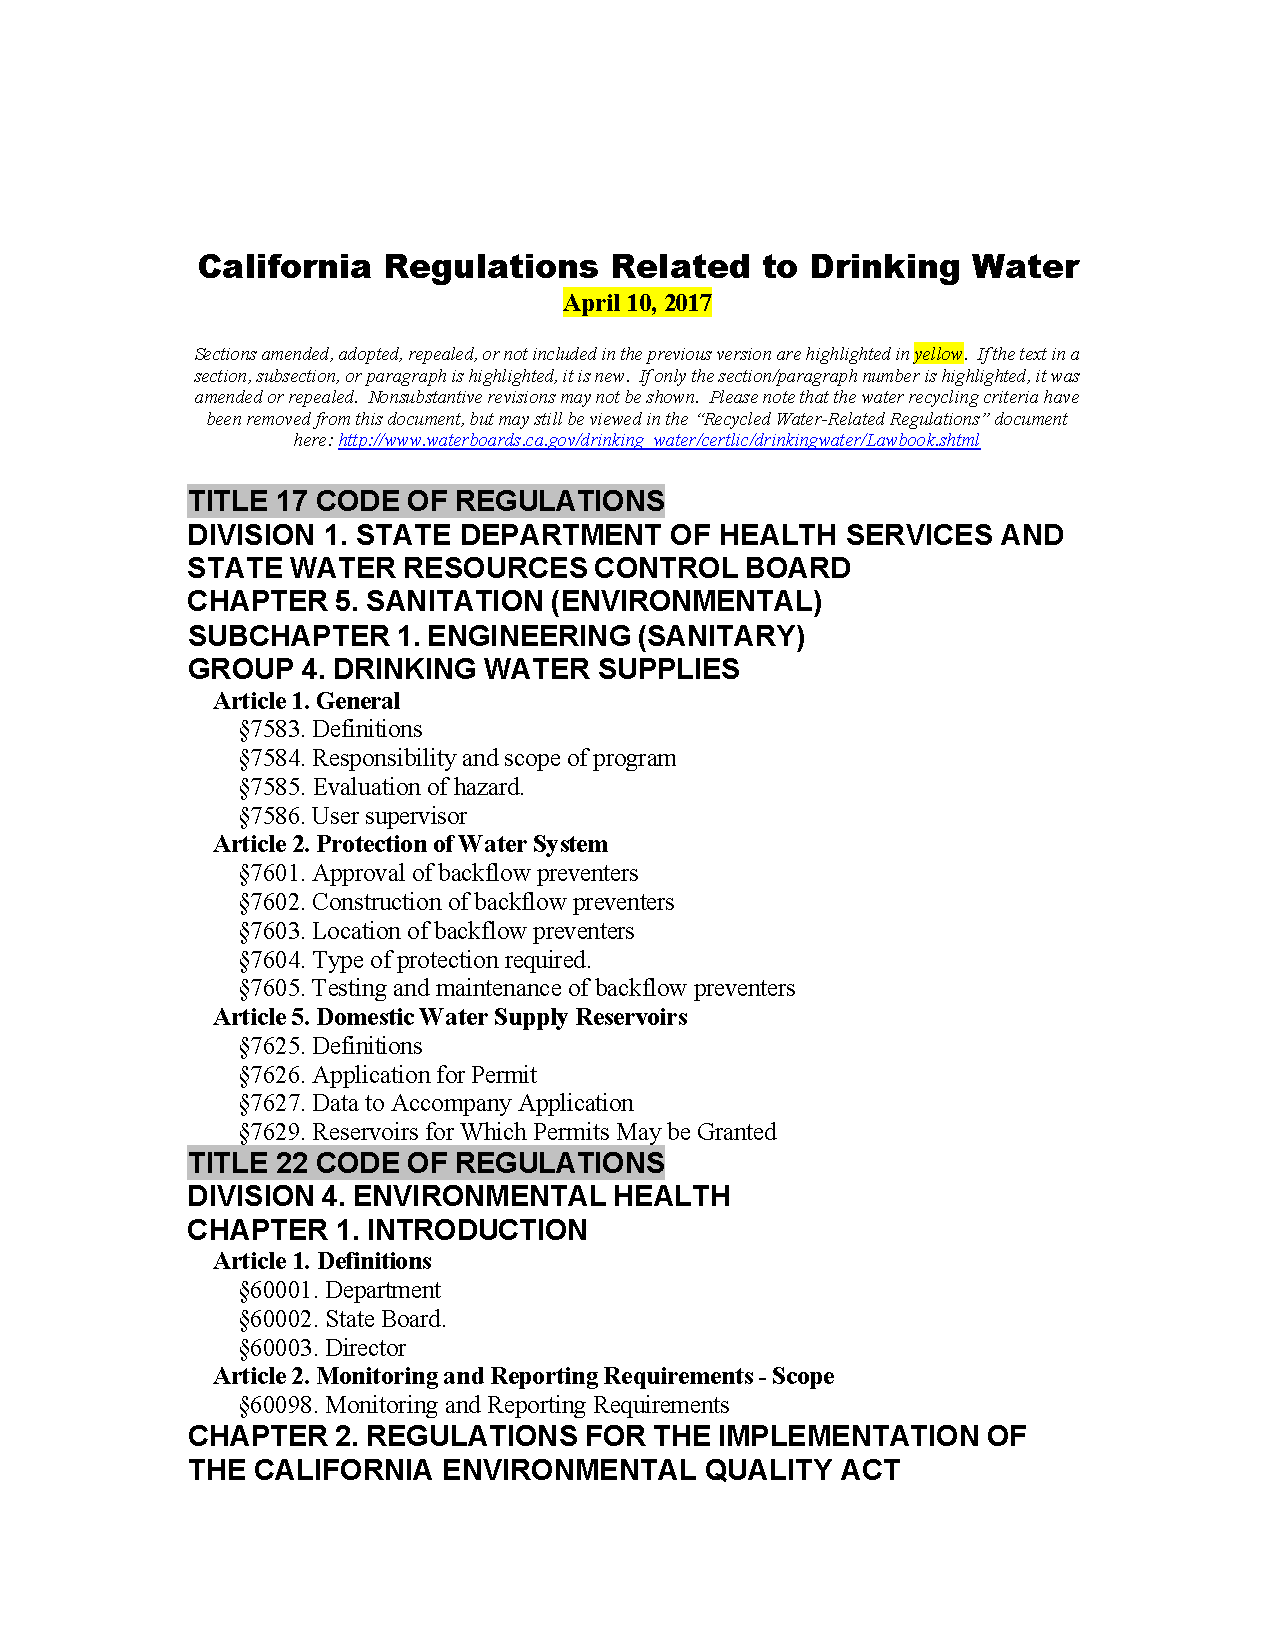
\includepdf[pages={1-12}]{CaliforniaDrinkingWaterRegulationsTOC}
%\newpage
%\thispagestyle{empty}
%\topskip0pt
%\vspace*{\fill}
%\begin{center}
%\textbf{American Water College - Water Treatment Operator Certification in California}
%\end{center}
%\vspace*{\fill}
%\newpage


%\newpage
%
%%\begin{dBox}
%%\lipsum*[1]
%%\end{dBox}
%
%
%% Please add the following required packages to your document preamble:
%% \usepackage{multirow}
%% \usepackage[table,xcdraw]{xcolor}
%% If you use beamer only pass "xcolor=table" option, i.e. \documentclass[xcolor=table]{beamer}
%\begin{table}[]
%\scriptsize
%\begin{tabular}{|p{2cm}|p{3cm}|p{3cm}|p{3cm}|}
%\hline
%\rowcolor[HTML]{1F15AD} 
%\multicolumn{1}{|c|}{\cellcolor[HTML]{1F15AD}{\color[HTML]{FFFFFF} Contaminant}} 
%
%& \multicolumn{1}{c|}{\cellcolor[HTML]{1F15AD}{\color[HTML]{FFFFFF} Maximum   Contaminant Level (MCL)}} 
%
%& \multicolumn{1}{c|}{\cellcolor[HTML]{1F15AD}{\color[HTML]{FFFFFF} Monitoring   Requirement – Surface Only or Combination}}                                                                                                                
%
%& \multicolumn{1}{c|}{\cellcolor[HTML]{1F15AD}{\color[HTML]{FFFFFF} Check Sampling,   Reporting and Public Notice}}                                                                                     \\ \hline
%                                                                                 & \textless{}40   samples/month, no more than 1 positive                                                &                                                                                                                                                                                                                                           & Repeat samples   are required for each coliform- positive sample. All samples must be   collected the same day.                                                                                       \\ \cline{2-2} \cline{4-4} 
%                                                                                 & \textgreater{}40 samples/month, no more than 5\%   positive.                                          &                                                                                                                                                                                                                                           & At least one   sample from same tap as original, another from an up- stream connection, and   one from downstream. All coliform positives must be tested for presence of   fecal coliform or E.coli.  \\ \cline{2-2} \cline{4-4} 
%
%
%\multirow{-3}{*}{Total coliform}                                                 &                                                                                                       
%
%& \multirow{-3}{*}{Compliance is based on  the presence or absence of total coliforms. All coliform positives must be   tested for presence of fecal coliform or E.coli. The total number of samples is based on the population   served.} & If repeat   sample is fecal coliform positive or if the original fecal coliform or E.coli   positive is followed by a total coliform positive, the state must be notified   on the same business day. \\ \hline
%                                                                                
%                                                                                 &                                                                                                       
%                                                                                 &                                                                                                                                                                                                                                           
%                                                                                 & Failure to meet   total percent inactivation on more than two days in a month is a violation.                                                                                                         \\ \cline{4-4} 
%
%\multirow{-2}{*}{Giardia Lamblis}                                                
%
%& \multirow{-2}{*}{3-Log (99.9\%) removal   or inactivation.}                                           & \multirow{-2}{*}{Based on calculated   residual disinfectant CT values.}                                                                                                                                                                  & State must be notified within one business day when disinfectant   residual is less than 0.2 mg/L.                                                                                                    \\ \hline
%Viruses                                                                          & 4-Log (99.99\%)   removal or inactivation                                                             &                                                                                                                                                                                                                                           & If residual is   less than 0.2 mg/L, then sampling must be every 4 hours until residual is   restored.                                                                                                \\ \hline
%\end{tabular}
%\end{table}



%\chapterimage{QuizCover} % Chapter heading image

% \chapter*{Regulations}
% \newpage
% \textbf{Match the following:}\\
% \begin{table}[ht]
% \renewcommand{\arraystretch}{2.4}
% \scriptsize
% \begin{tabular}{p{5cm}}
% A. Information Collection Rule                       \\

% B.  Long Term 1-Enhanced Surface Water Treatment Rule \\

% C.  Ground Water                                      \\

% D.  Stage 2-Disinfectant Byproduct Rule               \\

% E. Long Term 2-Enhanced Surface Water Treatment Rule \\

% F. Interim Enhanced Surface Water Treatment Rule     \\

% G. Disinfection/Disinfection Byproduct Rule, Phase I \\

% H. Total Coliform Rule                               \\

% I. Surface Water Treatment Rule                      \\

% \end{tabular}
% \renewcommand{\arraystretch}{1.2}
% \begin{tabular}{p{9cm}}
% i.  This   rule provides guidelines for identifying ground water sources at risk for   contamination and guidelines for taking corrective action.                                                                                                                                                \\
% \hline 
% ii.  This rule primarily addresses the reduction of risk from Cryptosporidium by limiting the   turbidity levels of filter effluents.                                                                                                                                                             \\
% \hline 
% iii.  This rule requires all systems serving fewer than 10,000 people   to achieve at least 99\% removal or inactivation of Cryptosporidium.                                                                                                                                                       \\
% \hline 
% iv.  This rule sets the monitoring and compliance requirements for   coliform bacteria.                                                                                                                                                                                                           \\
% \hline 
% v.  It required large public water suppliers to undertake monitoring   of microbial and disinfection byproducts in their water systems.                                                                                                                                                          \\
% \hline 
% vi.  This rule set maximum contaminant level goals and maximum   contaminant levels for trihalomethanes, five haleocetic acids, bromate and   chlorite.                                                                                                                                           \\
% \hline 
% vii.  This rule required all surface waters or ground waters under the   influence of surface waters to provide filtration and/or disinfection of the   source to meet 3 log removal or inactivation of Giardia   Lamblia cysts and 4 log removal or inactivation of   enteric viruses.           \\
% \hline 
% viii.  This rule is anticipated to propose treatment techniques to   improve control of microbial pathogens, specifically including Cryptosporidium. The techniques are   to consider the risks of treatment for Cryptospodrium   versus the potential for generation of   disinfection byproducts. \\
% \hline 
% ix.  The purpose of this rule is to assess information and research   that was not fully considered in the Stage 1 process or that has only been   available since 1998, as it relates to microbial standards to protect public   health.                                                        \\
% \hline 
% \end{tabular}
% \end{table}
% \textbf{Answers:}\\
% \begin{enumerate}[A.]
% \item \rule{1cm}{.5pt}
% \vspace{0.2cm}
% \item \rule{1cm}{.5pt}
% \vspace{0.2cm}
% \item \rule{1cm}{.5pt}
% \vspace{0.2cm}
% \item \rule{1cm}{.5pt}
% \vspace{0.2cm}
% \item \rule{1cm}{.5pt}
% \vspace{0.2cm}
% \item \rule{1cm}{.5pt}
% \vspace{0.2cm}
% \item \rule{1cm}{.5pt}
% \vspace{0.2cm}
% \item \rule{1cm}{.5pt}
% \vspace{0.2cm}\\
% \item \rule{1cm}{.5pt}
% \vspace{0.2cm}\\
% \end{enumerate}

% \newpage
% \textbf{Multiple Choice:}\\
\begin{enumerate}

\item Primary drinking water standards are set to protect the public from illnesses as a direct result in drinking water that exceeds maximum set levels. Secondary standards were set to alert the public to\\
a. the incidences of local cancer numbers\\
b. dissolved solids in water\\
c. immediate health concerns\\
d. radiological conditions concerning drinking water\\
e. *aesthetic issues with drinking water\\
\item A positive fecal coliform test must be reported to the primacy agency within\\
a. 8 hours.\\
b. 12 hours.\\
c. 24 hours.\\
d. 48 hours.\\
\item Which agency sets legal limits on the concentration levels of harmful contaminants in potable water distributed to customers?\\
a. National Primary Drinking Water Regulations\\
b. United States Environmental Protection Agency\\
c. United States Public Health Service\\
d. Occupational Health and Safety Organization\\
\item Which may be substituted for the analysis of residual disinfectant concentration, when total coliforms are also sampled at the same sampling point?\\
a. Heterotrophic plate count (HPC)\\
b. Fecal coliforms\\
c. Giardia lamblia\\
d. Combined chlorine\\
\item What does the acronym MCL stand for?\\
a. Minimum contaminant level\\
b. Micron contaminant level\\
c. Maximum contaminant level\\
d. Milligrams counted last\\
\item How long do sanitary surveys have to be retained for records?\\
a. 3 years\\
b. 5 years\\
c. 7 years\\
d. 10 years\\
\item The most severe water system violation that requires the fastest public notification\\
a. Tier I\\
b. Tier II\\
c. Tier III\\
d. Tier IV 8. The primacy agency may grant a variance or exemption as long as\\
a. The agency is using the Best Available Technology\\
b. There is no threat to public health\\
c. There is never a scenario for a variance or exemption\\
d. Both A. and B.\\
\item A public water system that serves at least 25 people six months out of the year\\
a. Nontransient noncommunity\\
b. Transient noncommunity\\
c. Community public water system\\
d. None of the above\\
\item Regulations based on the aesthetic quality of drinking water\\
a. Primary Standards\\
b. Secondary Standards\\
c. Microbiological Standards\\
d. Radiological Standards\\
\item The lowest reportable limit for a water sample\\
a. $0.5 \mathrm{mg} / 1$\\
b. Zero\\
c. Public health goal\\
d. Detection Level for reporting\\
\item Primary Standards are based on\\
a. Color and Taste\\
b. Aesthetic quality\\
c. Public Health\\
d. Odor\\
\item A disease causing microorganism\\
a. Pathogen\\
b. Colilert\\
c. Pathological\\
d. Turbidity\\
\item According to Surface Water Treatment Rule, what is the combined inactivation and removal for Giardia?\\
a. $1.0 \log s$\\
b. $2.0 \log \mathrm{s}$\\
c. $3.0 \log s$\\
d. 4.0 Logs\\
\item What is the equivalency expressed as a percentage for the SWTR inactivation and removal of viruses?\\
a. $99.9 \%$\\
b. $99.99 \%$\\
c. $99.0 \%$\\
d. $99.999 \%$\\
\item A water agency that takes more than 40 coliform samples must fall under what percentile?\\
a. $10 \%$\\
b. $7 \%$\\
c. $5 \%$\\
d. No positive samples allowable\\
\item The National Primary Drinking Water Regulations apply to drinking water contaminants that may have adverse effects on\\
a. Water color\\
b. Water taste\\
c. Water odor\\
d. Human health\\
\item Which of the following is considered an acute risk to health?\\
a. Two Tier 2 violations\\
b. One Tier 2 violation\\
c. Two Tier 1 violations\\
d. One Tier 1 violation\\
\item Records on turbidity analyses should be kept for a minimum of\\
a. 5 years\\
b. 7 years\\
c. 10 years\\
d. 25 years\\
\item Records on bacteriological analyses should be kept for a minimum of\\
a. 5 years\\
b. 7 years\\
c. 10 years\\
d. 25 years\\
\item Difference between primary and secondary standard substances:\\
a. Primary standards refer to substances that are carcinogenic, secondary standards do not.\\
b. Primary standards refer to substances that are thought to pose a threat to human health, secondary standards do not.\\
c. Primary standards refer to substances that, if not.put in check, will eventually kill humans, secondary standards do not.\\
d. Secondary qualities are aesthetic qualities and will only make some people sick, while primary standards refer to substances that will make everyone sick and may possibly cause death.\\
\item The SDWA defines a public water system that supplies piped water for human consumption as one that has\\
a. 10 service connection or serves 20 or more people for 60 or more days per year b. 15 service connections or serves 20 or more people for 90 or more days per year\\
c. 10 service connections or serves 25 or more people for 30 or more days per year\\
d. 15 service connections or serves 25 or more people for 60 or more days per year\\
\item According to the USEPA regulations, the owner or operator of a public water system that fails to comply with applicable\\
monitoring requirements shall give notice to the public within\\
a. 1 week of the violation in a letter hand-delivered to customers\\
b. 45 days of the violation by posting a notice at the town hall\\
c. 3 months of the violation in a daily newspaper in the area served by the system d. 1 year of the violation by including the notice with the water-bill .\\
\item What US agency establishes drinking water standards?\\
a. AWWA\\
b. USEPA\\
c. NIOSH\\
d. NSF\\
\item If a water supply exceeds the MCL, whose responsibility is it to notify the consumer?\\
a. the testing lab\\
b. the supplier\\
c. the DOH\\
d. the USEPA\\
\item According to the Lead and Copper Rule. the action for the 90th percentile lead level is:\\
a. $0.005 \mathrm{mg} / 1$\\
b. $0.015 \mathrm{mg} / \mathrm{l}$\\
c. $0.030 \mathrm{mg} / 1$\\
d. $0.050 \mathrm{mg} / \mathrm{l}$\\
\item The term "maximum contaminant level goal (MCLG)" means the:\\
a. Maximum allowable level of a given contaminant in drinking water\\
b. Level of a contaminant .in drinking water below which there are no known or suspected adverse health effects with a margin of safety\\
c. Level of a contaminant in drinking water that will trigger a Tier 1 violation\\
d. Minimum detectable level of a given contaminant\\
\item The maximum contaminant level goal (MCLG) of known or probable carcinogens is:\\
a. Set by the state\\
b. The same number as the maximum contaminant level (MCL)\\
c. Zero\\
d. The minimum detectable level of a given contaminant\\
\item The difference between Tier 1 and Tier 2 violations is:\\
a. Tier 1 violations-potentially impose-direct and adverse health effects; Tier 2 violations do not pose a direct threat to public health.\\
b. Tier 1 violations require public notification; Tier 2 violations do not require public notification\\ c. Tier 1 violations are acute; Tier 2 violations are not acute\\
d. Tier 1 violations have legal consequences; Tier 2 violations do not\\
\item The Safe Drinking Water Act requires to develop a comprehensive coliform monitoring plan\\
a. Large public water systems (serving $>50,000$ people)\\
b. Large and medium public water systems (serving $>3,300$ people)\\
c. Small and medium public water systems (serving $>25$ and $<3,300$ people)\\
d. All public water systems\\
\item The most important factor to consider in locating a well site from the health point of view is\\
a. Anticipated yield\\
b. Availability of electric power\\
c. Distance from other wells\\
d. Vulnerability\\
\item Trihalomethanes are classified as:\\
a. Metals\\
b. Inorganic constituents\\
c. Secondary drinking water standards\\
d. Radiological contaminants\\
e. Volatile organic compounds\\
\item The term "primacy" means the\\
a. Authority by the states to supersede USEPA drinking water regulations\\
b. Authority by the USEPA to supersede state drinking water regulations\\
c. Requirements for states to maintain drinking water regulations more stringent than USEPA regulations\\
d. Primary authority for implementation and enforcement of drinking water regulations\\
\item The Safe Drinking Water Act requires to develop a comprehensive coliform monitoring plan\\
a. Large public water systems (serving $>50,000$ people)\\
b. Large and medium public water systems (serving $>3,300$ people)\\
c. Small and medium public water systems (serving $>25$ and $<3,300$ people)\\
d. All public water systems\\
\item Contaminant monitoring requirements can depend on\\
a. The results of a vulnerability assessment\\
b. The size of the water system c. Previous maximum contaminant level (MCL) violations\\
d. All of the above\\
\item For public water systems using surface water and groundwater under the influence of surface water, turbidity must be measure at least\\
a. Every 4 hours\\
b. Daily\\
c. Weekly\\
d. Monthly\\
\item The difference between Tier 1 and Tier 2 violations is\\
a. Tier1-violations potentially impose-direct and adverse health effects; Tier 2 violations do not pose a direct threat to public health\\
b. Tier 1 violations require public notification; Tier 2 violations do not require public notification\\
c. Tier 1 violations are acute; Tier 2 violations are not acute\\
d. Tier 1 violations have legal consequences; Tier 2 violations do not\\
\item The maximum contaminant level goal (MCLG) of known or probable carcinogens is\\
a. Set by the state\\
b. The same number as the maximum contaminant level (MCL)\\
c. Zero\\
d. The minimum detectable level of a given contaminant\\
\item All of the following diseases may be transmitted by contaminated water, except for:\\
a. Cryptosporidiosis\\
b. Giardiasis\\
c. Cholera\\
d. Typhoid\\
e. Tuberculosis\\
\item The maximum disinfectant residual allowed in a distribution system is\\
a. $\quad 0.2 \mathrm{mg} / \mathrm{L}$\\
b. $\quad 2.0 \mathrm{mg} / \mathrm{L}$\\
c. $\quad 2.0 \mu \mathrm{g} / \mathrm{L}$\\
d. $4.0 \mathrm{mg} / \mathrm{L}$\\
e. There is no maximum disinfectant residual standard\\
\item What steps must be taken when a single routine sample tests positive for total coliform? a. Immediately notify the Department of Health Services\\
b. Immediately notify customers\\
c. Re-test a new sample taken from the original sample point\\
d. Re-test a new sample taken from the original sample point, plus at points immediately upstream and downstream\\
e. Flush the system around the original sample point to re-establish disinfectant levels\\
\item For drinking water distribution systems with over 40 routine coliform samples per month, the maximum amount of coliform-positive samples permitted is\\
a. 2\\
b. $2 \%$\\
c. 5\\
d. $5 \%$\\
e. variable, depending on the size of the system\\
\item Final determination of vulnerability is made by\\
a. Private contractor/consultants\\
b. The primacy agency\\
c. The water supplier\\
d. All of the above\\
\item The regulation that establishes standards for microbiological quality in drinking water is a. The Disinfection By-Product Rule\\
b. Secondary Drinking Water Standards\\
c. The Total Coliform Rule\\
d. The Lead and Copper Rule\\
e. Maximum Contaminant Level\\
\item Primary and secondary drinking water standards are normally established with a\\
a. Maximum contaminant level\\
b. Minimum contaminant level\\
c. Public health goal\\
d. Maximum contaminant level goal\\
e. Minimum contaminant level goal\\
\item The presence of coliform bacteria in a distribution system\\
a. Is positive proof that pathogenic organisms are present\\
b. Indicates that chlorine demand has increased dramatically c. Indicates that pathogenic organisms may be present also\\
d. Requires the use of brilliant green bile as a secondary disinfectant\\
e. Has no particular significance\\
\item The regulation that establishes standards for microbiological quality in drinking water is\\
a. The Disinfection By-Product Rule\\
b. Secondary Drinking Water Standards\\
c. The Total Coliform Rule\\
d. The Lead and Copper Rule\\
e. Maximum Contaminant Level\\
\item For public water systems using surface water and groundwater under the influence of surface water, turbidity must be measured at least\\
a. Every 4 hours\\
b. Daily\\
c. Weekly.\\
d. Monthly\\
\item Contaminant monitoring requirements can depend on\\
a. The results of a vulnerability assessment\\
b. The size of the water system\\
c. Previous maximum contaminant level (MCL) violations\\
d. All of the above\\
\item According to the Lead and Copper Rule. the action for the 90th percentile lead level is:\\
a. $0.005 \mathrm{mg} / \mathrm{l}$\\
b. $0.015 \mathrm{mg} / \mathrm{l}$\\
c. $0.030 \mathrm{mg} / \mathrm{l}$\\
d. $0.050 \mathrm{mg} / \mathrm{l}$\\
\item The difference between Tier 1 and Tier 2 violations is\\
a. Tier 1-violations potentially impose-direct and adverse health effects; Tier 2 violations do not pose a direct threat to public health\\
b. Tier 1 violations require public notification; Tier 2 violations do not require public notification\\
c. Tier 1 violations are acute; Tier 2 violations are not acute\\
d. Tier 1 violations have legal consequences; Tier 2 violations do not\\
\item For public water systems using surface water and groundwater under the influence of surface water, turbidity must be measure at least\\
a. Every 4 hours\\
b. Daily\\
c. Weekly.\\
d. Monthly\\
\item Contaminant monitoring requirements can depend on\\
a. The results of a vuilnerability assessment\\
b. The size of the water system\\
c. Previous maximum contaminant level (MCL) violations\\
d. All of the above\\
\item The Safe Drinking Water Act requires to develop a comprehensive coliform monitoring plan a. Large public water systems (serving $>50,000$ people)\\
b. Large and medium public water systems (serving $>3,300$ people)\\
c. Small and medium public water systems (serving $>25$ and $<3,300$ people)\\
d. All public water systems 
 \item BARF is an acronym for\\
a) Boil Advisory Reference Form\\
*b) Bacteriological Analysis Report Forms\\
c) Biological Activity Reactive Format\\
d) vomit\\
  \item Which of these does NOT have a primary MCL?\\
a) nitrate\\
b) fluoride\\
*c) manganese\\
d) copper\\
  \item MCLG is an acronym for\\
a) Most Common Lucky Guess\\
b) Minimum Colloidal Level Goals\\
c) Maximum Chlorine Level Gallons\\
*d) Maximum Contaminant Level Goals\\
  \item The LT2ESWTR has decreed that we test our source water for the presence of\\
a) algae\\
b) pharmaceuticals\\
*c) cryptosporidium\\
d) nitrate\\
  \item Combined filter effluent must be less than NTU in $95 \%$ of all measurements (collected every four hours) for each month.\\
a) $1.0 \mathrm{NTU}$\\
b) $2.0 \mathrm{NTU}$\\
c) $3.0 \mathrm{NTU}$\\
*d) $0.3 \mathrm{NTU}$\\
  \item If you get a positive coliform sample what must be done?\\

a) retake the original sample\\
*b) retake the original sample plus one sample within five upstream service connections and one sample within five downstream service connections.\\
c) retake the original sample, one from the water plant, and one from any service connection close to the original sample site.\\
d) since no fecal coliform was detected, no more sampling needs to take place.\\
\item All systems in Kentucky must carry at least ppm chlorine residual everywhere in their system.\\
*a) 0.2\\
b) 2.0\\
c) 4.0\\
d) there is no minimum\\

\item For a community water system, a sanitary survey is required to be conducted \rule{1.5cm}{0.5pt}\\

a. Every five years\\
b. Every two years\\
*c. Every three years\\
d. Every 10 years

  \item Primary drinking water standards are set to protect the public from illnesses as a direct result in drinking water that exceeds maximum set levels. Secondary standards were set to alert the public to\\
a. the incidences of local cancer numbers\\
b. dissolved solids in water\\
c. immediate health concerns\\
d. radiological conditions concerning drinking water\\
e. *aesthetic issues with drinking water\\

  \item What is the reason for keeping adequate, reliable records in a treatment plant?\\
*a. to record the plant's effectiveness and because of requirements by regulatory agencies\\
b. to maintain records for cold cases\\
c. in case the IRS wishes to check files for due diligence\\
d. because of homeland security issues and files being available to the public\\

\item Which of the following substances pose an immediate health threat whenever standards are exceeded?\\
a.	Benzene and mercury\\
*b.	Coliform and nitrate\\
c.  Mercury and coliform\\
d.  Lead and nitrate\\
\end{enumerate}



\newpage
%\chapterimage{QuizCover} 
% \chapter*{Treatment}
\begin{enumerate}
\item What is the purpose of coagulation and flocculation?\\
a. control corrosion\\
b. to kill disease causing organisms\\
c. to remove leaves, sticks, and fish debris\\
d. *to remove particulate impurities and suspended matter\\
\item How are filter production (capacity) rates measured?\\
a. Mgd/sq.ft.\\
b. $* \mathrm{Gpm} / \mathrm{sq} . \mathrm{ft}$.\\
c. $\mathrm{Gpm}$\\
d. Mgd\\
\item Why should a filter be drained if it is going to be out-of-service for a prolonged period?\\
a. to allow the media to dry out\\
b. to save water\\
c. to prevent the filter from floating on groundwater levels\\
d. *to avoid algal growth\\
\item Which of the following are commonly used coagulation chemicals?\\
a. hypochlorites and free chlorine\\
b. sodium and potassium chlorides\\
c. *alum and polymers\\
d. bleach and HTH\\
\item How can an operator tell if a filter is NOT completely cleaned after backwashing?\\
a. *the initial headloss is on the high side\\
b. the backwash rate was too slow\\
c. mudballs are NOT present\\
d. backwashing pumping rate is too low\\
\item Flocculation is defined as\\
a. *the gathering of fine particles after coagulation by gentle mixing\\
b. clumps of bacteria\\
c. the capacity of water to neutralize acids\\
d. a high molecular weight of compounds that have negative charges\\
\item A multi-barrier water filtration plant that contains a flash mix, a coagulation/flocculation zone, sedimentation, filtration and a clear well is considered to be a\\
a. community special treatment plant\\
b. direct filtration plant\\
c. reverse osmosis plant\\
d. *conventional filtration plant\\
e. traditional plant\\
\item The filtration unit process usually\\
a. is located at the beginning of a filtration plant\\
b. *follows the coagulation/flocculation/sedimentation processes\\
c. is located after the clear well area\\
d. is located on the plant effluent line after the clearwell\\
\item Filters are generally backwashed when the loss-of-head indicator registers a certain set value, such as 6-ft, or upon a certain time, say 48-hours, or upon a rise in\\
a. alkalinity\\
b. a jar-test result\\
c. *turbidity\\
d. temperature\\
\item What is a method of reducing hardness?\\
a. *Softening\\
b. Hardening\\
c. Lightning\\
d. Flashing\\
\item The solid that adsorbs a contaminant is called the:\\
a. *Adsorbent\\
b. Adsorbate\\
c. Sorbet\\
d. Rock\\
\item The adsorption process is used to remove:\\
a. *Organics or inorganics\\
b. Bugs or salts\\
c. Organisms or dirt\\
d. Color or particles\\
\item Describe two primary methods used to control taste and odor?\\
a. *Oxidation and adsorption\\
b. Filtration and sedimentation\\
c. Mixing and coagulation\\
d. Sedimentation and clarification\\
\item What is the recommended loading rate for copper sulfate for algae control at an alkalinity greater than $50 \mathrm{mg} / \mathrm{L}$ ?\\
a. $0.9 \mathrm{lb}$ of copper sulfate per acre of surface area\\
b. $1.9 \mathrm{lb}$ of copper sulfate per acre of surface area\\
c. 2-4 lb of copper sulfate per acre of surface area\\
d. $.4 \mathrm{lb}$ of copper sulfate per acre of surface area\\
\item The basic goal for water treatment is to\\
a. Protect public health\\
b. Make it clear\\
c. Make it taste good\\
d. Get stuff out\\
\item Greensand can be operated in either regeneration or regeneration modes.\\
a. Continuous or intermittent\\
b. Fast or slow\\
c. Hot or cold\\
d. Constant or unusual\\
\item The two most common types of chlorine disinfection by-products include:\\
a. TTHM and HAA5\\
b. TTHA of HMM5\\
c. Turbidity and color\\
d. Chloride and fluoride\\
\item GAC contactors are used to reduce the amount of contaminants in water.\\
a. Inorganic\\
b. Turbidity\\
c. Particle\\
d. Organic\\
\item List the five types of surface water filtration systems.\\
a. Bag filtration, cartridge filtration, fine filtration, coarse filtration, media filtration\\
b. Conventional treatment, direct filtration, slow sand filtration, diatomaceous earth filtration, membrane filtration\\
c. Turbidity filtration, color filtration, bag filtration, fine filtration, media filtration\\
d. None of the above\\
\item Describe two primary methods used to control taste and odor?\\
a. Oxidation and adsorption\\
b. Filtration and sedimentation\\
c. Mixing and coagulation\\
d. Sedimentation and clarification\\
\item The adsorption process is used to remove:\\
a. Organics or inorganics\\
b. Bugs or salts\\
c. Organisms or dirt\\
d. Color or particles\\
\item The solid that adsorbs a contaminant is called the:\\
a. Adsorbent\\
b. Adsorbate\\
c. Sorbet\\
d. Rock\\
\item What is a method of reducing hardness?\\
a. Softening\\
b. Hardening\\
c. Lightning\\
d. Flashing\\
\item Bag and cartridge filters are used to remove which two pathogenic microorganisms?\\
a. Viruses and giardia\\
b. Giardia and cryptosporidium\\
c. Viruses and bacteria\\
d. None of the above\\
\item The process of cleaning a filter by pumping water up through the filter media is called the filter.\\
a. Backwashing\\
b. Rewashing\\
c. Purging\\
d. Lifting\\
\item In a typical water treatment plant, alum would be added into the mixer.\\
a. Speed\\
b. Large\\
c. Slow\\
d. Flash\\
\item When comparing conventional treatment with direct filtration, what process unit is in the conventional treatment plant that is not in the direct filtration plant?\\
a. Filter\\
b. Clarifier\\
c. Mixer\\
d. Detention\\
\item List the basic processes, in the proper order, for a conventional treatment plant.\\
a. Coagulation, flocculation, sedimentation, filtration\\
b. Flocculation, coagulation, sedimentation, filtration\\
c. Filtration, coagulation, flocculation, sedimentation\\
d. Coagulation, sedimentation, flocculation, filtration 31. The four most common oxidants include:\\
a. Chlorine, potassium permanganate, ozone, chlorine dioxide\\
b. Chlorides, soap, air, coagulants\\
c. Air, chemicals, sodium, chloride\\
d. Flocculants, coagulants, sediments, granules\\
\item When operating a filter, one of the operational concerns is the difference between the pressure or head on top of the filter and the pressure or head at the bottom of the filter. This difference is called pressure.\\
a. Different\\
b. Differential\\
c. High\\
d. Low\\
\item What type of polymer is used to improve the efficiency of the sedimentation process?\\
a. Cationic\\
b. Nonionic\\
c. Anionic\\
d. All of the above\\
\item A(n)\_ polymer is commonly used as a coagulant.\\
a. Anionic\\
b. Cationic\\
c. Nonionic\\
d. Ionic\\
\item $\mathrm{A}(\mathrm{n}) \ldots$ polymer is used to enhance flocculation.\\
a. Anionic\\
b. Cationic\\
c. Nonionic\\
d. Ionic\\
\item $\mathrm{Al}_{2}\left(\mathrm{SO}_{4}\right)_{3} \cdot 18 \mathrm{H}_{2} \mathrm{O}$ is the chemical formula for:\\
a. Alum\\
b. Iron\\
c. Manganese\\
d. Lead\\
\item Particles that are less than $1 \mu \mathrm{m}$ in size and will not settle easily and are called:\\
a. Light particles\\
b. Colloidal particles\\
c. Colored particles\\
d. Flat particles\\
\item The sedimentation portion of water treatment is also called a(n):\\
a. Clarifier\\
b. Filter\\
c. Adsorber\\
d. Water treater\\
\item Slowly agitating coagulated materials is the process of:\\
a. Flocculation\\
b. Coagulation\\
c. Sedimentation\\
d. Filtration\\
\item The process of decreasing the stability of colloids in water is called:\\
a. Flocculation\\
b. Coagulation\\
c. Sedimentation\\
d. Clarification\\
\item The chemical oxidation process in water treatment is typically used to aid in the removal of :\\
a. Organic contaminants\\
b. Inorganic contaminants\\
c. Large contaminants\\
d. None of the above\\
\item Flocculation, sedimentation, filtration, and adsorption are processes.\\
a. Physical\\
b. Chemical\\
c. Biological\\
d. Mechanical\\
\item Oxidation, coagulation, and disinfection are\\
a. Physical\\
b. Chemical\\
c. Biological\\
d. Mechanical\\
\item A precipitate can be formed after which one of the following processes:\\
a. Oxidation\\
b. Flocculation\\
c. Filtration\\
d. Adsorption\\
\item Water that is safe to drink is called water.\\
a. Potable\\
b. Palatable\\
c. Good\\
d. Clear\\
\item The type of organisms that can cause disease are said to be microorganisms.\\
a. $\mathrm{Bad}$\\
b. Pathogenic\\
c. Undesirable\\
d. Sick\\
\item The basic goal for water treatment is to\\
a. Protect public health\\
b. Make it clear\\
c. Make it taste good\\
d. Get stuff out\\
\item Four types of aesthetic contaminants in water include the following:\\
a. Odor, turbidity, color, hydrogen sulfide gas\\
b. Pathogens, microorganisms, arsenic, disinfection by-products\\
\item What does $\mathrm{mg} / \mathrm{L}$ stand for?\\
a. Microorganisms/Liter\\
b. Milligrams/Loser\\
c. Milligrams/Liter\\
d. None of the above\\
\item Disinfection by-products are a product of:\\
a. Filtration\\
b. Disinfection\\
c. Sedimentation\\
d. Adsorption\\
\item Acute contaminants are those that can cause sickness after:\\
a. Prolonged exposure\\
b. Low levels or low exposure\\
\item Chronic contaminants are those that can cause sickness after:\\
a. Prolonged exposure\\
b. Low levels or low exposure\\
\item TTHMs and HAA5s can affect:\\
a. Health\\
b. Aesthetics\\
c. Color\\
d. Odor\\
\item Oxidation, coagulation, and disinfection are processes.\\
a. Physical\\
b. Chemical\\
c. Biological\\
d. Mechanical\\
\item Flocculation, sedimentation, filtration, and adsorption are processes.\\
a. Physical\\
b. Chemical\\
c. Biological\\
d. Mechanical\\
\item A precipitate can be formed after which one of the following processes:\\
a. Oxidation\\
b. Flocculation\\
c. Filtration\\
d. Adsorption\\
\item Giardia and cryptosporidium are a type of:\\
a. Mineral\\
b. Organism\\
c. Color\\
d. Bird\\
\item The chemical oxidation process in water treatment is typically used to aid in the removal of :\\
a. Organic contaminants\\
b. Inorganic contaminants\\
c. Large contaminants\\
d. None of the above\\
\item The process of decreasing the stability of colloids in water is called:\\
a. Flocculation\\
b. Coagulation\\
c. Sedimentation\\
d. Clarification\\
\item Slowly agitating coagulated materials is the process of:\\
a. Flocculation\\
b. Coagulation\\
c. Sedimentation\\
d. Filtration\\
\item The sedimentation portion of water treatment is also called a(n):\\
a. Clarifier\\
b. Filter\\
c. Adsorber\\
d. Water treater\\
\item Particles that are less than $1 \mu \mathrm{m}$ in size and will not settle easily and are called:\\
a. Light particles\\
b. Colloidal particles\\
c. Colored particles\\
d. Flat particles\\
\item One micrometer is also equal to:\\
a. $0.1 \mathrm{~mm}$\\
b. $0.0001 \mathrm{~mm}$\\
c. $0.001 \mathrm{~mm}$\\
d. $1 \mathrm{~m}$\\
\item Particles less than $0.45 \mu \mathrm{m}$ in size are considered to be:\\
a. Dissolved\\
b. Really little\\
c. Colored particles\\
d. Flat particles\\
\item Turbidity is measured as:\\
a. $\mathrm{Mg} / \mathrm{L}$\\
b. $\mathrm{mL}$\\
c. $\mathrm{gpm}$\\
d. NTU\\
\item $\mathrm{Al} 2(\mathrm{SO} 4) 3 \cdot 18 \mathrm{H} 20$ is the chemical formula for:\\
a. Alum\\
b. Iron\\
c. Manganese\\
d. Lead\\
\item $\mathrm{A}(\mathrm{n}) \_$polymer is commonly used as a coagulant.\\
a. Anionic\\
b. Cationic\\
c. Nonionic\\
d. Ionic\\
\item A(n)\_polymer is used to enhance flocculation.\\
a. Anionic\\
b. Cationic\\
c. Nonionic\\
d. Ionic\\
\item The concentration of a chemical added to the water is measured in:\\
a. $\mathrm{mL}$\\
b. $\mathrm{mg}$\\
c. $\mathrm{mg} / \mathrm{L}$\\
d. Liters\\
\item The quantity of chlorine remaining after primary disinfection is called a residual.\\
a. Chlorine\\
b. Permaganate\\
c. Hot\\
d. Cold\\
\item Primary disinfectants are used to microorganisms.\\
a. Hurt\\
b. Inactivate\\
c. Burn up\\
d. Evaporate\\
\item Secondary disinfectants are used to provide a in the distribution system.\\
a. Color\\
b. Chemical\\
c. Smell\\
d. Residual\\
\item What type of polymer is used to improve the efficiency of the sedimentation process?\\
a. Cationic\\
b. Nonionic\\
c. Anionic\\
d. All of the above\\
\item When operating a filter, one of the operational concerns is the difference between the pressure or head on top of the filter and the pressure or head at the bottom of the filter. This difference is called pressure.\\
a. Different\\
b. Differential\\
c. High\\
d. Low\\
\item List the basic processes, in the proper order, for a conventional treatment plant.\\
a. Coagulation, flocculation, sedimentation, filtration\\
b. Flocculation, coagulation, sedimentation, filtration\\
c. Filtration, coagulation, flocculation, sedimentation\\
d. Coagulation, sedimentation, flocculation, filtration\\
\item The four most common oxidants include:\\
a. Chlorine, potassium permanganate, ozone, chlorine dioxide\\
b. Chlorides, soap, air, coagulants\\
c. Air, chemicals, sodium, chloride\\
d. Flocculants, coagulants, sediments, granules\\
\item When comparing conventional treatment with direct filtration, what process unit is in the conventional treatment plant that is not in the direct filtration plant?\\
a. Filter\\
b. Clarifier\\
c. Mixer\\
d. Detention\\
\item In a typical water treatment plant, alum would be added into the mixer.\\
a. Speed\\
b. Large\\
c. Slow d. Flash\\
\item The process of cleaning a filter by pumping water up through the filter media is called \_ the filter.\\
a. Backwashing\\
b. Rewashing\\
c. Purging\\
d. Lifting\\
\item Bag and cartridge filters are used to remove which two pathogenic microorganisms?\\
a. Viruses and giardia\\
b. Giardia and cryptosporidium\\
c. Viruses and bacteria\\
d. None of the above\\
\item List the four types of membrane filtration processes commonly used in water treatment.\\
a. MF, UF, NF, and RO\\
b. MNF, UOF, NOF, and ROO\\
c. CFM, FM, FN, and OR\\
d. None of the above\\
\item What is a method of reducing hardness?\\
a. Softening\\
b. Hardening\\
c. Lightning\\
d. Flashing\\
\item Adsorption of a substance involves its accumulation onto the surface of a:\\
a. Solid\\
b. Rock\\
c. Pellet\\
d. Snow ball\\
\item The solid that adsorbs a contaminant is called the:\\
a. Adsorbent\\
b. Adsorbate\\
c. Sorbet\\
d. Rock\\
\item The adsorption process is used to remove:\\
a. Organics or inorganics\\
b. Bugs or salts\\
c. Organisms or dirt\\
d. Color or particles\\
\item Describe two primary methods used to control taste and odor?\\
a. Oxidation and adsorption\\
b. Filtration and sedimentation\\
c. Mixing and coagulation\\
d. Sedimentation and clarification\\
\item List the five types of surface water filtration systems.\\
a. Bag filtration, cartridge filtration, fine filtration, coarse filtration, media filtration\\
b. Conventional treatment, direct filtration, slow sand filtration, diatomaceous earth filtration, membrane filtration\\
c. Turbidity filtration, color filtration, bag filtration, fine filtration, media filtration\\
d. None of the above\\
\item GAC contactors are used to reduce the amount of contaminants in water.\\
a. Inorganic\\
b. Turbidity\\
c. Particle\\
d. Organic\\
\item Greensand can be operated in either regeneration or regeneration modes.\\
a. Continuous or intermittent\\
b. Fast or slow\\
c. Hot or cold\\
d. Constant or unusual\\
\item What is the cause of taste and odor problems in raw surface water?\\
a. Copper sulfate\\
b. Blue-green algae\\
c. Oxygen\\
d. Lake turnover\\
\item What chemical reduces blue-green algae growth?\\
a. Chlorine\\
b. Caustic Soda\\
c. Copper Sulfate\\
d. Alum\\
\item What is the purpose of adding fluoride to drinking water?\\
a. Increase tooth decay\\
b. Reduce tooth decay\\
c. Make teeth white\\
d. Government conspiracy\\
\item The optimal coagulant dose is determined by a\\
a. Chlorine Test\\
b. Flocculation test\\
c. Jar Test\\
d. Coagulation test\\
\item The most common primary coagulant is\\
a. Alum\\
b. Cationic polymer\\
c. Fluoride\\
d. Anionic polymer\\
\item Bacteria and Viruses belong to a particle size known as\\
a. Suspended\\
b. Dissolved\\
c. Strained\\
d. Colloidal\\
\item The purpose of coagulation is to\\
a. Increase filter run times\\
b. Increase sludge\\
c. Increase particle size\\
d. Destabilize colloidal particles\\
\item The purpose of flocculation\\
a. Destabilize colloidal particles\\
b. Increase particle size\\
c. Decrease sludge\\
d. Decrease filter run times\\
\item Primary coagulant aids used in treatment process are\\
a. Poly-aluminum chloride\\
b. Aluminum sulfate\\
c. Ferric chloride\\
d. All of the Above\\
\item How do water agencies monitor the effectiveness of their filtration process?\\
a. Alkalinity\\
b. Conductivity\\
c. Turbidity\\
d. $\mathrm{pH}$\\
\item Flocculation is used to enhance\\
a. Number of particle collisions to increase floc\\
b. Charge neutralization\\
c. Dispersion of chemicals in water\\
d. Settling speed of floc\\
\item If there is a problem with floc formation, what would you consider changing?\\
a. Adjust coagulant dose\\
b. Stay the course\\
c. Adjust mixing intensity\\
d. Both $A \& C$\\
\item Which step in the treatment process is the shortest?\\
a. Filtration\\
b. Sedimentation\\
c. Flocculation\\
d. Coagulation\\
\item To lower the $\mathrm{pH}$ for enhanced coagulation the operator will add\\
a. Chlorine\\
b. Sulfuric acid\\
c. Lime\\
d. Caustic Soda\\
\item The flocculation process lasts how long?\\
a. Seconds\\
b. 5-10 minutes\\
c. 15-45 minutes\\
d. Over an hour\\
\item The function of a flocculation basin is to\\
a. Settle colloidal particles\\
b. Destabilize colloidal particles\\
c. Mix chemicals\\
d. Allow suspended particles to grow\\
\item The treatment process that involves coagulation, flocculation, sedimentation, and filtration is known as\\
a. Direct filtration\\
b. Slow sand Filtration\\
c. Conventional treatment\\
d. Pressure filtration\\
\item Sedimentation produces waste known as\\
a. Backwash water\\
b. Sludge\\
c. Waste water\\
d. Mud\\
\item What kind of process is the sedimentation step?\\
a. Physical\\
b. Chemical\\
c. Biological\\
d. Direct\\
\item The weirs at the effluent of a sedimentation basin are also called\\
a. Effluent weirs\\
b. Baffling\\
c. Launders\\
d. Spokes\\
\item Sedimentation is used in water treatment plants to\\
a. Settle pathogenic material\\
b. Destabilize particles\\
c. Disinfect water\\
d. Reduce loading on Filters\\
\item Scouring is a term that describes conditions in a sedimentation tank which\\
a. Could impact the rest of treatment process\\
b. Higher flow rates in the sludge zone\\
c. Re-suspends settle sludge\\
d. All of the above\\
\item The four zones in a Sedimentation basin include\\
a. Inlet, sedimentation, sludge, outlet\\
b. Inlet, filter, waste, outlet\\
c. Inlet, top, bottom, outlet\\
d. Surface, sedimentation, sludge, outlet\\
\item The removal and inactivation requirement for Giardia is?\\
a. $99.9 \%$\\
b. $99.99 \%$\\
c. $99.00 \%$\\
d. $90 \%$\\
\item Short circuiting in a sedimentation basin could be caused by\\
a. Surface wind\\
b. Ineffective weir placement, or weirs covered in algae\\
c. Poor baffling in sedimentation inlet zone\\
d. All of the Above\\
\item How much solids should be removed during sedimentation?\\
a. $95 \%$ or more\\
b. $80-95 \%$\\
c. $70-80 \%$\\
d. $60-70 \%$\\
\item The type of basin that includes coagulation and flocculation is\\
a. Rectangular\\
b. Triangular\\
c. Up-Flow\\
d. None of the above\\
\item Recarbonation basins are used to stabilize water after\\
a. Filtration\\
b. Disinfection\\
c. Softening\\
d. Coagulation\\
\item Which of the following is an effective way for removing iron water? a. adding baffles\\
b. adding sodium chloride\\
c. aeration and filtration\\
d. flash mixing\\
\item How can iron bacteria be controlled in a water distribution system?\\
a. by aeration\\
b. filtration\\
c. chlorination\\
d. precipitation\\
\item Which of the following is a hazard when handling hydrofluosilicic acid?\\
a. fire\\
b. explosion\\
c. corrosion\\
d. inhalation\\
\item Trihalomenthane may be partially removed from water by:\\
a. fluoridation\\
b. chlorination\\
c. oxidation\\
d. ultraviolet radiation\\
\item Which of the following forms of iron is most soluble in water?\\
a. Ferric $\left(\mathrm{Fe}^{+3}\right)$\\
b. Ferric hydroxide $\left[\mathrm{Fe}\left(\mathrm{OH}_{3}\right)\right]$\\
c) Ferrous $\left(\mathrm{Fe}^{+2}\right)$\\
d. Ferrous oxide $(\mathrm{FeO})$\\
\item Two fundamental treatment requirements for public water systems using surface sources are\\
a. Coagalat1on and sedimentation\\
b. Lime softening and disinfection\\
c. Filtration and aeration\\
d. Disinfection and filtration\\
\item A zeolite softening unit will replace calcium and magnesium ions with ions.\\
a. Fluoride\\
b. Iron\\
c. Sodium\\
d. Sulfur\\
\item One use of polyphosphates is to:\\
a. Control algae\\
b. Improve taste\\
c. Sequester iron and manganese\\
d. Kill bacteria 124. An acceptable means of corrosion control for relatively small systems is\\
a. Activated carbon\\
b. Lime-soda ash softening\\
c. $\mathrm{pH}$ control\\
d. zeolite softening\\
\item Which of the following chemicals will most likely keep iron in suspension?\\
a. Chlorine\\
b. Fluoride\\
c. Polyphosphate\\
d. Lime inhibitor\\
\item Lead in drinking water can result in\\
a. Impaired mental functioning in children\\
b. Prostate cancer in men\\
c. Stomach and intestinal disorders\\
d. Reduced white blood cell count\\
\item If raw water turbidity changed from 10 to 300 turbidity units and the finished water turbidity had increased from 0.1 to 1.0 turbidity units, the unit process having the most impact to correct this situation is\\
a. Coagulation\\
b. Sedimentation\\
c. Filtration\\
d. Disinfection\\
\item The problem caused by dissolved carbon dioxide in the water of the distribution system is\\
a. increased Trihalomethanes\\
b. Corrosion\\
c. Excessive encrustation\\
d. Tastes and odors\\
\item The presence of the coliform group of bacteria in water indicates\\
a. Contamination\\
b. Inadequate disinfection\\
c. Improper sampling\\
d. Taste and odor problems\\
\item The granular filtration process is designed to reduce\\
a. Calcium and magnesium sulfates\\
b. True color\\
c. Total dissolved solids\\
d. Turbidity\\
\item The presence of the coliform group of bacteria in water indicates\\
a. Contamination\\
b. Inadequate disinfection\\
c. Improper sampling\\
d. Taste and odor problems\\
\item Aeration in water treatment plants is used to\\
a. Lower the $\mathrm{pH}$\\
b. Reduce concentrations of dissolved gasses\\
c. Reduce turbidity\\
d. Stabilize chlorine residuals\\
\item What can the operator do if iron fouling appears to be a problem in an ion exchange softener?\\
a. Decrease the strength of the brine used in the regeneration stage\\
b. Increase backwash flow rates\\
c. Inçrease duration of backwash stage\\
d. Increase duration of service stage\\
\item At what $\mathrm{pH}$ would a chlorinated water have the highest concentration of hypochlorous acid?\\
a. 5\\
b. 7\\
c. 9\\
d. 11\\
\item One use of polyphosphates is to\\
a. Control algae\\
b. Improve taste\\
c. Sequester iron and manganese\\
d. Kill bacteria\\
\item What happens when lime is fed to water for corrosion control?\\
a. Alkalinity is decreased\\
b. CO2 does not change\\
c. Turbidity is decreased\\
d. $\mathrm{pH}$ is increased\\
\item The main characteristic of raw water that enables algae to grow is\\
a. Presence of copper sulfate\\
b. Low $\mathrm{pH}$\\
c. High hardness\\
d. Presence of nutrients\\
\item The type of corrosion caused by the use of dissimilar metal in a water system is\\
a. Caustic corrosion\\
b. Galvanic corrosion\\
c. Oxygen corrosion\\
d. Tubercular corrosion\\
\item A zeolite softening unit will replace calcium and magnesium ions with ions.\\
a. Fluoride\\
b. Iron\\
c. Sodium\\
d. Sulfur\\
\item Two fundamental treatment requirements for public water systems using surface sources are\\
a. Coagulation and sedimentation\\
b. Lime softening and disinfection\\
c. Filtration and aeration\\
d. Disinfection and filtration\\
\item A method used to soften water is\\
a. Aeration\\
b. Sedimentation\\
c. Ion exchange\\
d. Adsorption\\
\item The main characteristic of raw water that enables algae to grow is\\
a. Presence of copper sulfate\\
b. Low $\mathrm{pH}$\\
c. High hardness\\
d. Presence of nutrients\\
\item What happens when lime is fed to water for corrosion control?\\
a. Alkalinity is decreased\\
b. $\mathrm{CO}_{2}$ does not change\\
c. Turbidity is decreased\\
d. $\mathrm{pH}$ is increased\\
\item Which of the following chemicals will most likely keep iron in suspension?\\
a. Chlorine\\
b. Fluoride\\
c. Polyphosphate\\
d. Lime inhibitor\\
\item If raw water turbidity changed from 10 to 300 turbidity units and the finished water turbidity had increased from 0.1 to 1.0 turbidity units, the unit process having the most impact to correct this situation is\\
a. Coagulation\\
b. Sedimentation\\
c. Filtration\\
d. Disinfection\\
\item The granular filtration process is designed to reduce\\
a. Calcium and magnesium sulfates\\
b. True color\\
c. Total dissolved solids\\
d. Turbidity\\
\item Aeration in water treatment plants is used to\\
a. Lower the $\mathrm{pH}$\\
b. Reduce concentrations of dissolved gasses\\
c. Reduce turbidity\\
d. Stabilize chlorine residuals\\
\item What can the operator do if iron fouling appears to be a problem in an ion exchange softener?\\
a. Decrease the strength of the brine used in the regeneration stage\\
b. Increase backwash flow rates\\
c. Inçrease duration of backwash stage\\
d. Increase duration of service stage\\
\item Trihalomenthane may be partially removed from water by:\\
a. fluoridation\\
b. chlorination\\
c. oxidation\\
d. ultraviolet radiation\\
\item Temporary cloudiness in a freshly drawn sample of tap water may be caused by:\\
a. air\\
b. chlorine\\
c. hardness\\
d. silica\\
\item Two fundamental treatment requirements for public water systems using surface sources are\\
a. Coagulation and sedimentation\\
b. Lime softening and disinfection\\
c. Filtration and aeration\\
d. Disinfection and filtration\\
\item A zeolite softening unit will replace calcium and magnesium ions with ions.\\
a. Fluoride\\
b. Iron\\
c. Sodium\\
d. Sulfur\\
\item What happens when lime is fed to water for corrosion control? a. Alkalinity is decreased\\
b. $\mathrm{CO}_{2}$ does not change\\
c. Turbidity is decreased\\
d. $\mathrm{pH}$ is increased\\
\item Which two chemicals are used to remove turbidity?\\
a. Soda Ash and lime\\
b. Copper sulphate and caustic soda\\
c. Alum and lime\\
\item Which of the following is considered to be a coagulant aid?\\
a. Lime\\
b. Polymer\\
c. Bentonite\\
d. All of the above\\
\item Alum precipitates as\\
a. Aluminum carbonate\\
b. Aluminum sulphate\\
c. Aluminum hydroxide\\
\item Turbidity removal with alum is best accomplished at what $\mathrm{pH}$ ?\\
a. 3.5\\
b. 5.0\\
c. 6.5\\
\item Which of the following will not lower the $\mathrm{pH}$ ?\\
a. Alum\\
b. Carbonic acid\\
c. Ferric chloride\\
d. Sodium carbonate\\
\item Liquid fluoride is delivered as:\\
a. Sodium Fluoride\\
b. Hydrofluorosilicic acid\\
c. Sodium Silicofluoride\\
d. Hydrofluoric acid\\
\item An upflow clarifier will have which of the following processes?\\
a. Coagulation\\
b. Flocculation\\
c. Sedimentation\\
d. All of the above\\
\item Sludge that rises to the surface of a sedimentation basin is caused by:\\
a. Not removing sludge often enough\\
b. Removing sludge too often\\
c. $\mathrm{pH}$ is too low\\
d. Surface loading rate is too low\\
\item Pin floc leaving a sedimentation basin may indicate a problem with:\\
a. Coagulation\\
b. Flocculation\\
c. Sedimentation\\
d. Disinfection\\
\item What is the backwash rate for a rapid sand filter?\\
a. 2 gpm/sq.ft.\\
b. $15 \mathrm{gpm} / \mathrm{sq} . \mathrm{ft}$.\\
c. $20 \mathrm{gpm} / \mathrm{sq} . \mathrm{ft}$.\\
d. $25 \mathrm{gpm} / \mathrm{sq} . \mathrm{ft}$.\\
\item What is the maximum run time for a gravity filter?\\
a. 8 hours\\
b. 20 hours\\
c. 48 hours\\
d. 100 hours\\
\item During backwash, the filter bed should expand:\\
a. $5-10 \%$\\
b. $15-20 \%$\\
c. $30-50 \%$\\
d. $60-80 \%$\\
\item If the backwash time is too short, what may result?\\
a. Too much freeboard\\
b. Mudballs\\
c. Loss of filter media\\
d. Filter breakthrough\\
\item If the filtration rate is too high, what may result?\\
a. Filter breakthrough\\
b. Mudballs\\
c. Reduction in operating costs\\
d. Lower headloss\\
\item Solids removed from a filter are most commonly removed by what method?\\
a. Adsorption\\
b. Straining\\
c. Deactivation\\
d. Flocculation\\
\item What is a typical filtration rate for slow sand filters?\\
a. 2.0-6.0 GPM/sq. ft.\\
b. 6.0-10.0 GPM/sq. ft.\\
c. $1.0-2.0 \mathrm{GPM} / \mathrm{sq}$. ft.\\
*d. $0.5-0.10 \mathrm{GPM} / \mathrm{sq}$. ft.\\
\item In a typical conventional treatment plant, the finished water turbidity for an individual filter should be less than\\
a. 1.0 NTUs\\
*b. 0.3 NTUs\\
c. $5.0 \mathrm{NTUs}$\\
d. 3.0 NTUs\\
\item A filter running under normal conditions will see head loss in a filter\\
a. Remain constant\\
b. Increase slowly\\
c. Rapidly increase\\
d. Decrease slowly\\
\item A filter must be washed if this condition is met\\
a. Head Loss\\
b. Turbidity break through\\
c. Maximum Filter run time\\
d. All of the Above\\
\item Filter performance is measured by the removal of\\
a. Oxygen\\
b. Head loss\\
c. Turbidity\\
d. Chlorine\\
\item What is the biologically active layer of a slow sand filter called?\\
a. Mixed Media\\
b. Duel Media\\
c. Sludge Layer\\
d. Schmutzdecke\\
\item The pressure drop in a filter is called\\
a. Turbidity breakthrough\\
b. Head Loss\\
c. Filtration\\
d. Backwash\\
\item What is the most common reason for putting a filter into the wash cycle?\\
a. Head loss\\
b. Filter run time\\
c. Turbidity breakthrough\\
d. Water level decrease\\
\item Formation of mud balls and excessive boiling during a wash is an indicator of\\
a. Proper backwash rate\\
b. Too low backwash rate\\
c. Excessive backwash rate\\
d. Improper chemical dose\\
\item Important processes which occur during filtration are\\
a. Sedimentation\\
b. Adsorption\\
c. Straining\\
d. All of the Above\\
\item Typical filtration rates for a conventional treatment plant are\\
a. 0.2-0.6 GPM/sq.ft.\\
b. 2.0-10.0 GPM/sq.ft.\\
c. 10.0-20.0 GPM/sq.ft.\\
d. 200-400 GPM/sq.ft.

 \item Detention time in flocculation basins are usually designed to provide for\\
a. 5 to 15 minutes.\\
*b. 15 to 45 minutes.\\
c. 45 to 60 minutes.\\
d. 60 to 90 minutes.\\
  \item Alum works best in a pH range of\\
a. less than 4.0.\\
b. 4.0 to 5.5 .\\
*c. 5.8 to 8.5 .\\
d. Greater than 9.0.\\
  \item Which statement is true concerning colloidal particles?\\
*a. Colloidal particles are so small that gravity has little effect on them\\
b. The zeta potential between colloidal particles is balanced by covalent bonding\\
c. Electrical phenomenon of colloidal particles predominate and control their behavior\\
d. The surface area of colloidal particles is very small compared to their mass\\
  \item Which natural electrical force keeps colloidal particles apart in water treatment?\\
a. van der Waals forces\\
b. Ionic forces\\
*c. Zeta potential\\
d. Quantum forces\\
  \item The zeta potential measures the number of excess all particulate matter.\\
*a. electrons\\
b. ions\\
c. cations\\
d. protons\\
\end{enumerate}
\section{Sample Questions for Level II, Answers on Page 157}
\begin{enumerate}[label=TII-\arabic*]
  \item Low temperature water can be compensated for when using alum by\\
a. increasing the pH.\\
b. decreasing the pH.\\
*c. increasing the alum dosage.\\
d. decreasing the alum dosage.\\
  \item Which is the optimal pH range for the removal of particulate matter, when using alum as a coagulant?\\
a. 4.5 to 5.7\\
b. 5.8 to 6.5\\
*c. 6.5 to 7.2\\
d. 7.3 to 8.1\\
  \item Which forces will pull particles together once they have been destabilized in the coagulation-flocculation process?\\
*a. van der Waals forces\\
b. Zeta potential\\
c. Ionic forces\\
d. Quantum forces\\
  \item Which is a common mistake that operators make in regards to flocculation units?\\
a. Excessive flocculation time\\
b. Lack of food-grade NSF-approved grease on the flocculator bearings\\
*c. Keeping the mixing energy the same in all flocculation units\\
d. Too short a flocculation time\\
  \item Ferric sulfate has which advantage over aluminum sulfate (alum)?\\
a. Less staining characteristics\\
b. Less cost\\
*c. More dense floc\\
d. Not as corrosive\\
\end{enumerate}
\section{Sample Questions for Level III, Answers on Page 157}
\begin{enumerate}[label=TIII-\arabic*]
  \item How much alkalinity as CaCO$_{3}$ will dry-basis alum consume?\\
*a. 0.5 mg/l\\
b. 0.8 mg/l\\
c. 1.2 mg/l\\
d. 1.5 mg/l\\
  \item Natural zeolites that have become exhausted with use are regenerated by immersing them in a strong solution of which chemical?\\
*a. NaCl\\
b. NaOH\\
c. HCl\\
d. H$_2$SO$_4$ \\
\item The zeta potential on a particular sample of water is -2 . The degree of coagulation is best described as\\
a. poor.\\
b. fair.\\
*c. excellent.\\
d. maximum.\\
  \item Which is a disadvantage of using static mixers?\\
a. They do not provide good mixing\\
b. They are not economical\\
*c. They increase head loss\\
d. They require too much maintenance\\
  \item Which is the usual effective pH range of iron salt coagulants?\\
*a. 3.5 to 9.0\\
b. 6.5 to 8.8\\
c. 3.0 to 9.5\\
d. 4.2 to 9.0\\
\end{enumerate}
\section{Sample Questions for Level IV, Answers on Page 158}
\begin{enumerate}[label=TIV-\arabic*]
  \item Which is the minimum recommended number of flocculation basins?\\
a. 2\\
*b. 3\\
c. 4\\
d. 5\\
  \item Which type of polymer(s) is (are) sometimes formulated with regulated substances from the following list?\\
a. Polyethylene\\
b. Divinylbenzene\\
c. Polypropylene and polyethylene\\
*d. Nonionic and anionic polymers\\
  \item Which is the most probable solution if rotifers are visible in the finished water?\\
a. Superchlorinate the water plant\\
*b. Optimize coagulation, flocculation, and filtration\\
c. Use aeration followed by lime softening before the settling process\\
d. Use oxygen deprivation\\
  \item The best addition for water that is highly colored due to organic matter would be\\
a. the addition of lime.\\
b. lime addition with increase in the coagulant being used.\\
c. a small increase in a nonionic polymer.\\
*d. the addition of an acid to lower pH before coagulation.\\
  \item If the activation process of silica is not carefully controlled,\\
a. the silica could splash due to high heat of reactants.\\
*b. it could inhibit floc formation.\\
c. it could corrode and destroy the metal and rubber in the flocculators.\\
d. it could deposit silica on the flocculators and the gears, bringing it eventually to a grinding halt.\\
\end{enumerate}
\section{Monitor, Evaluate, \& Adjust Treatment Processes-Clarification and Sedimentation}
\section{Sample Questions for Level I, Answers on Page 158}
\begin{enumerate}[label=TI\arabic*]

  \item In solid-contact basins with fairly constant water quality parameters, how often should the solids concentration be determined?\\
a. At least once per week\\
b. At least every other day\\
c. At least once per month\\
*d. At least twice per day\\
  \item The definition of decant is\\
a. to draw off a liquid layer from a vessel of any size without disturbing any layer(s) above or below.\\
b. to draw off the sediment at the bottom of a vessel of any size without disturbing the overlying liquid layer(s).\\
c. to remove the precipitate at the bottom of any size vessel.\\
*d. to draw off the liquid from a vessel of any size without stirring up bottom sediment.\\
  \item How often should sedimentation basins with mechanical sludge removal equipment be drained and inspected?\\
a. Twice a year\\
*b. Once a year\\
c. Every other year\\
d. Every three years\\
  \item Which is the most important reason to reduce turbidity?\\
a. To reduce taste and odor problems\\
*b. To remove pathogens\\
c. To reduce corrosion\\
d. To determine the efficiency of coagulation and filtration\\
\end{enumerate}
\section{Sample Questions for Level II, Answers on Page 159}
\begin{enumerate}[label=TII-\arabic*]
  \item If enteric disease-causing protozoans have been found in the effluent of a water plant, which is the most probable solution?\\
a. Where possible, use powdered activated carbon (PAC) throughout water plant; backwashing filters will remove the PAC\\
b. Use PAC only in the sedimentation basin; backwashing the filters will remove the PAC\\
*c. Use multibarrier approach—coagulation, flocculation, sedimentation, and filtration\\
d. Superchlorinate the water plant \\
\item Which is the major cause of short circuiting in a sedimentation basin?\\
a. Open basins that are subject to algal growths and thick slime growths on the side of the basin\\
b. Basins without a wind break\\
*c. Poor inlet baffling\\
d. Density currents\\
  \item Conventional sedimentation has a removal of Cryptosporidium oocysts.\\
*a. less than 0.5-log\\
b. 0.5-log\\
c. 1.0-log\\
d. 2.0-log\\
  \item In solids-contact basins, the weir loading normally should not exceed weir length.\\
a. 1 gpm/ft\\
b. 2 gpm/ft\\
c. 5 gpm/ft\\
*d. 10 gpm/ft\\
  \item Dissolved-air flotation is particularly good for removing\\
a. sulfides.\\
b. inorganics.\\
c. manganese and iron.\\
*d. algae.\\
\end{enumerate}
\section{Sample Questions for Level III, Answers on Page 159}
\begin{enumerate}[label=TIII-\arabic*]
  \item Which determines whether or not colloidal-sized particles in suspension repel each other, stay in suspension, or agglomerate and eventually settle?\\
a. Number of collisions\\
b. Flow and temperature of the water\\
c. Types of chemical bonding\\
*d. Magnitude of the charges\\
  \item If the sludge in a sedimentation basin becomes too thick, which could happen?\\
a. Gases from decomposition will rise through the settled sludge accelerating normal floc settling\\
b. Abundant trihalomethanes and haloacetic acids will form\\
*c. Solids can become resuspended or taste and odors can develop\\
d. The sludge will compact at the bottom of the basin making it very difficult to remove\\
  \item In basins using tube and plate settlers, which parameter must be much better than conventional treatment basins?\\
a. Metals must be oxidized before reaching the tubes and plates\\
b. Floc rate must be 2 to 3 times slower than conventional basins\\
c. Floc rate must be 3 to 4 times faster than conventional basins\\
*d. Floc must have good settling characteristics \\
\item Which type of sedimentation basins have the flow of water admitted at an angle?\\
a. Rectangular settling basins\\
b. Square settling basins\\
c. Center-feed settling basins\\
*d. Spiral-flow basins\\
  \item At which minimum angle must self-cleaning tube settlers be placed?\\
*a. 50 degrees\\
b. 60 degrees\\
c. 65 degrees\\
d. 70 degrees\\
\end{enumerate}
\section{Sample Questions for Level IV, Answers on Page 160}
\begin{enumerate}[label=TIV-\arabic*]
  \item If nematodes are interfering with the disinfectant, which is the most probable solution?\\
*a. Optimize the settling process\\
b. Use chloramines\\
c. Decrease detention time of finished water in clearwell and tanks\\
d. Use oxygen deprivation\\
  \item At which angle should the parallel inclined plates be installed when using the shallow-depth sedimentation method?\\
a. $35^{\circ}$\\
*b. $45^{\circ}$\\
c. $50^{\circ}$\\
d. $60^{\circ}$\\
  \item Why do solids-contact basins have much shorter detention times than conventional treatment basins?\\
a. Because chemical reactions take place throughout the basin\\
b. Because the settling zone water moves upward, while at the same time the mixing zone moves upward\\
c. Because the gentle upward flow of the water throughout the basin is conducive for producing larger settleable floc\\
*d. Because of the recycled materials from the sludge blanket, the chemical reactions occur more quickly and completely in the mixing area\\
  \item The pulsating energy in a pulsator clarifier helps to\\
*a. maintain a uniform sludge blanket layer.\\
b. mix the coagulants with the raw water.\\
c. mix the coagulant aids with the primary coagulant and water to help in flocculation.\\
d. raise the sludge blanket over the weir for wasting.\\
  \item Pulsator clarifiers are used to treat water that is\\
a. low in temperature, usually $<10^{\circ} \mathrm{C}$.\\
*b. high in color and low in turbidity.\\
c. low in color and high in turbidity.\\
d. high in organic acids.\\
\end{enumerate}
\section{Monitor, Evaluate, \& Adjust Treatment Processes-Filtration}
\section{Sample Questions for Level I, Answers on Page 160}
\begin{enumerate}[label=TI\arabic*]
  \item Which is the filtration flow rate through a manganese greensand pressure filter?\\
a. 1 to $2 \mathrm{gpm} / \mathrm{ft}^{2}$\\
*b. 2 to $3 \mathrm{gpm} / \mathrm{ft}^{2}$\\
c. 3 to $5 \mathrm{gpm} / \mathrm{ft}^{2}$\\
d. 5 to $8 \mathrm{gpm} / \mathrm{ft}^{2}$\\
  \item When a filter is ripening,\\
a. it is in need of a backwash.\\
b. turbidity is just starting to break through.\\
*c. it is becoming more efficient in particle removal.\\
d. it is beginning to grow algae in the filter bed, walls, and troughs.\\
  \item Virgin greensand can be regenerated by soaking the filter bed for several hours in a solution of chlorine containing\\
a. $50 \mathrm{mg} / \mathrm{L} \mathrm{Cl}_{2}$.\\
b. $\quad 75 \mathrm{mg} / \mathrm{L} \mathrm{Cl}_{2}$.\\
*c. $\quad 100 \mathrm{mg} / \mathrm{L} \mathrm{Cl}_{2}$.\\
d. $200 \mathrm{mg} / \mathrm{L} \mathrm{Cl}_{2}$.\\
  \item Which role does the action of straining of suspended particles play during filtration?\\
*a. Minor\\
b. Fair\\
c. Good\\
d. Major\\
  \item The turbidity of settled water before it is applied to the filters (post sedimentation process) should always be kept below\\
*a. 1 to $2 \mathrm{ntu}$.\\
b. 2 to $4 \mathrm{ntu}$.\\
c. 5 ntu.\\
d. 8 to $10 \mathrm{ntu}$.\\
\end{enumerate}
\section{Sample Questions for Level II, Answers on Page 160}
\begin{enumerate}[label=TII-\arabic*]
  \item Which is the best process for the removal of turbidity?\\
a. Anion exchange\\
*b. Coagulation, flocculation, sedimentation, and filtration\\
c. Chemical oxidation\\
d. Granular activated carbon\\
  \item If filter run times between backwashes are long, for example one week, because high quality (low turbidity) water is being applied to the filters, which problem could still arise?\\
a. Mudball formation\\
b. Air binding and formation of mudballs\\
c. Extended backwashing due to media becoming too compacted\\
*d. Floc breakthrough \\
\item Gravel displacement in a filter bed from backwash rates with too high of a velocity could eventually cause\\
a. compaction of the filter media.\\
b. loss of media into the backwash troughs.\\
*c. a sand boil.\\
d. bed shrinkage.\\
  \item Virgin greensand\\
a. does not require regeneration.\\
*b. requires regeneration with potassium permanganate - 1 hour soak with 60 grams KMnO4\\
c. requires regeneration with manganese dioxide - 2 hour soak with 25\% by weight solution of MnO2\\
d. requires regeneration with manganese hydroxide - 4 hour soak with 200 grams Mn(OH)2)\\
  \item Which conventional treatment step is eliminated by direct filtration?\\
a. Oxidation\\
b. Aeration\\
c. Flocculation\\
*d. Sedimentation\\
\end{enumerate}
\section{Sample Questions for Level III, Answers on Page 161}
\begin{enumerate}[label=TIII-\arabic*]
  \item If crustaceans have clogged the water treatment plant's filters, which is the most probable solution?\\
a. Shut down the filters and physically remove them\\
b. Shut down one filter at a time and drain; once the crustaceans have died, physically remove them and then repeat process on the other filters\\
c. Backwash filters using a very high concentration of ozone in the water\\
*d. Use a disinfectant that targets the specific organisms in question\\
  \item Which organism can escape coagulation and thus pass through a granular filter?\\
a. Giardia\\
b. Entamoeba\\
*c. Cryptosporidium\\
d. Naegleria\\
  \item Reverse osmosis membranes will compact faster with\\
a. higher iron content.\\
b. higher chlorine contact.\\
*c. higher pressure.\\
d. higher pH.\\
  \item Which would immediately occur if newly installed manganese greensand was not skimmed of the fines after backwashing and stratification steps were completed?\\
a. Uneven flow through the bed\\
b. Cracks would develop in the bed\\
c. Mudball formation\\
*d. Shorter filter runs \\
\item When a filter is operated at normal flow rates, its ability to trap flocculated particles in suspension is a function of\\
a. effective size multiplied by uniformity coefficient.\\
b. effective size multiplied by uniformity coefficient divided by media size.\\
*c. media depth and media size.\\
d. media depth and uniformity coefficient.\\
\end{enumerate}
\section{Sample Questions for Level IV, Answers on Page 161}
\begin{enumerate}[label=TIV-\arabic*]
  \item Which is the best solution if iron bacteria are causing corrosion problems in the filters?\\
a. Protect the metal parts of the filters by adding zinc orthophosphate\\
b. Optimize the settling process\\
*c. Superchlorinate\\
d. Add lime at 50 mg/L to one filter at a time\\
  \item A conventional water treatment plant with dual media filters has very cold water in the winter and warm water in the summer. Which should the operator do to compensate for this temperature change?\\
a. Use more coagulants in the summer per million gallons\\
*b. Sustain the same bed expansion without media loss by reducing or increasing backwash flow rate\\
c. Increase summer bed expansion and increase winter backwash flow rates\\
d. Increase bed expansion in the winter compared to summer in order to remove turbidity\\
  \item How are reverse osmosis membranes cleaned once they become fouled?\\
a. They are soaked in high purity industrial soap for at least 24 hours\\
*b. They are cleaned with an acid wash\\
c. They are cleaned with an acid, then with an industrial soap for 24 hours\\
d. They are cleaned first with a high purity industrial soap and then soaked in an acid solution for 3 days\\
  \item Which membrane process is used to treat brackish water or seawater?\\
a. Microfiltration\\
b. Nanofiltration\\
*c. Reverse osmosis\\
d. Ultrafiltration\\
  \item The amount of reject water from a reverse osmosis unit is dependent on the number of stages in which the membranes are configured and the\\
*a. feed pressure.\\
b. amount of cations.\\
c. amount of cations and anions.\\
d. pH of the water.\\
\end{enumerate}
\section{Monitor, Evaluate, and Adjust Treatment Processes-Residuals Disposal}
\section{Sample Questions, General, Answers on Page 162}
\begin{enumerate}[label=TG-\arabic*]
  \item In the precipitative softening plant, which percentage of solids sludge is produced?\\
a. 1\%\\
*b. 5\%\\
c. 10\%\\
d. 30\%\\
  \item Which sludge disposal method is most economical for lime-soda ash softening plants?\\
a. Disposal into the sewage system\\
b. Sand drying beds\\
*c. Lagoons\\
d. Landfill the sludge\\
  \item Current regulations require water treatment wastes to be monitored\\
*a. daily.\\
b. weekly.\\
c. monthly.\\
d. quarterly.\\
  \item Which process is used to concentrate sludge?\\
a. Sand bed\\
b. Solar lagoon\\
*c. Thickener\\
d. Centrifuge\\
  \item Which process is used to dewater sludge?\\
a. Wash water basin\\
c. Thickener\\
*b. Sand bed\\
c. Thickener\\
d. Reclamation basin\\
\end{enumerate}
\section{Sample Questions for Level III, Answers on Page 162}
\begin{enumerate}[label=TIII-\arabic*]
  \item Which is the total concentration of dissolved solids in the wastewater from the regeneration of ion exchange units?\\
a. $\quad 10,000$ to $20,000 mg/l$\\
b. 20,000 to 30,000 mg/l\\
*c. 35,000 to 45,000 mg/l\\
d. 45,000 to 60,000 mg/l\\
  \item Which is the usual range of percent sludge solids, if the sludge is allowed to accumulate and compact at the bottom of a sedimentation basin?\\
*a. 2-4 \%\\
b. 4-7 \%\\
c. 7-12 \%\\
d. 12-15 \% \\
\item Which should be determined first before an in-ground sedimentation tank is drained?\\
a. The solids content\\
b. The hazardous metals content\\
c. Sludge volume and volume of process area to make sure it will be large enough\\
*d. Water table level\\
  \item Which sludge dewatering process is best for alum sludges (which are difficult to dewater) when the cakes are very dry, filtrate is clear, and solids capture is very high?\\
a. Centrifuge\\
b. Vacuum filters\\
*c. Filter press\\
d. Belt filter press\\
  \item Which sludge dewatering process requires a precoat of diatomaceous earth and its use has declined due to other newer methods?\\
a. Centrifuge\\
*b. Vacuum filters\\
c. Filter press\\
d. Belt filter press\\
 \item Which precipitates can foul a cation exchange resin?\\
a. Sodium chloride and potassium chloride\\
b. Chlorate and borate\\
c. Sulfates\\
*d. Iron and manganese\\
  \item Which process works best for sequestering manganese?\\
a. Sodium silicate alone\\
b. Sodium silicate and chlorine\\
c. Polyphosphates alone\\
*d. Polyphosphates and chlorine\\
  \item When should polyphosphates used for sequestration of iron and manganese from a well be injected into the process?\\
a. Right after disinfection\\
b. Immediately after aeration to remove unwanted gases\\
c. Right after clarification\\
*d. Right after the water leaves the well\\
  \item Recarbonation is\\
*a. adding CO2 to the water.\\
b. adding bicarbonate to the water.\\
c. adding acid to precipitate the excess lime.\\
d. adding caustic soda.\\
  \item In the ion-exchange softening process, once the resin can no longer soften water it must be\\
a. renewed.\\
b. re-catalyzed.\\
*c. regenerated.\\
d. recharged.\\
\end{enumerate}
\section{Sample Questions for Level II, Answers on Page 164}
\begin{enumerate}[label=TII-\arabic*]
  \item Ion exchange processes can typically be used for direct groundwater treatment as long as turbidity and levels are not excessive.\\
a. calcium carbonate\\
*b. iron\\
c. carbon dioxide\\
d. sodium sulfate \\
\item Softened water has a high pH and a high concentration of CaCO$_{3}$. Therefore, stabilization is essential in order to prevent the CaCO$_{3}$ from precipitating out\\
a. in household plumbing.\\
b. in the clear well.\\
c. in the distribution system.\\
*d. on the filters.\\
  \item Which is the best type of salt to use in the regeneration of ion exchange softener resin?\\
a. Fine-grained salt\\
b. Block salt\\
c. Block or road salt\\
*d. Rock salt or pellet-type salt\\
  \item Powdered activated carbon is primarily used to control\\
a. disinfectant by-products.\\
*b. organic compounds responsible for tastes and odors.\\
c. synthetic organic chemicals.\\
d. humic and fulvic acids.\\
  \item Ion exchange will remove\\
*a. all hardness.\\
b. all hardness down to 7.4 mg/l, as CaCO3.\\
c. all hardness down to 17.2 mg/l, as CaCO3.\\
d. all hardness down to about 25.0 mg/l, as CaCO3.\\
\end{enumerate}
\section{Sample Questions for Level III, Answers on Page 164}
\begin{enumerate}[label=TIII-\arabic*]
  \item It is impossible to produce waters with a hardness of less than \_\_\_ when using the lime-soda ash process.\\
a. 9 mg/l\\
b. 17 mg/l \\
*c. 25 mg/l \\
d. 50 mg/l \\
  \item When added to water for softening purposes, soda ash will do which of the following?\\
*a. Disinfect the water and kill the vast majority of protozoans, viruses, bacteria, and other multicellular organisms\\
b. Raise the pH of water to between 8.0 and 9.8 pH units\\
c. Add CO2 to the water\\
d. Add calcium alkalinity to the water\\
  \item Magnetic ion exchange resin has been developed to remove\\
*a. total organic carbon.\\
b. chlorides.\\
c. iron and magnesium.\\
d. sulfates and sulfides. 
  \item Approximately how much carbon is lost during the reactivation process for granular activated carbon?\\
*a. 5 \%\\
b. 7 \%\\
c. 10 \%\\
d. 15 \%\\
  \item Which is the most advantageous application point for powdered activated carbon?\\
*a. Raw water intake\\
b. After coagulation\\
c. After oxidation with chlorine\\
d. In the filters\\
\end{enumerate}
\section{Sample Questions for Level IV, Answers on Page 165}
\begin{enumerate}[label=TIV-\arabic*]
  \item Which is the most effective method for removing tastes and odors?\\
a. Coagulation, sedimentation, and filtration\\
*b. Granular activated carbon\\
c. Anion exchange\\
d. Lime softening\\
  \item Backwashing rate procedures should be reassessed to determine the cause of granular activated carbon loss if the loss per year exceeds\\
*a. 2 inches.\\
b. 4 inches.\\
c. 6 inches.\\
d. 8 inches.\\
  \item Which is the most efficient process for the removal of nitrite and nitrate?\\
a. Powdered activated carbon\\
b. Granular activated carbon\\
*c. Anion exchange\\
d. Cation exchange\\
  \item Which is the main problem if particle agglomeration is occurring in a filter for iron and manganese removal at the interface of the coal layer and the layer below?\\
a. Oxidant is too weak\\
b. Coagulant dosage is excessive\\
c. Coal layer is too fine\\
*d. Coal layer is too coarse\\
  \item Which is the most effective method for the removal of disinfection by-products?\\
a. Reverse osmosis\\
b. Lime softening\\
c. Ultrafiltration\\
*d. Granular activated carbon\\
\end{enumerate}
\begin{enumerate}
  \item are used to cause particles to become destabilized and begin to clump together.\\
a) coagulant aids\\
b) nonsettable solids\\
c) zeta particles\\
*d) primary coagulants\\
 \item The purpose of stabilization is\\
a) to prevent floc from rising in the basin\\
b) to prevent sludge from entering the filters\\
*c) to prevent corrosion or excessive scale from entering the distribution system\\
d) to prevent excessive turbidity at the top of the filters\\
  \item Core sampling is a viable way to check the condition of your\\
a) raw water\\
b) coagulation process\\
c) finished water\\
*d) filters\\
 \item In solid contact units, the three main operational fundamentals are\\
a) sedimentation, slurry, \& suspended solids\\
b) mixing, clarifying, \& filtration\\
*c) chemical dosage, recirculation rate, \& sludge control\\
d) weighing agents, alkalinity \& pac\\
  \item Particle counters can be used in place of \rule{1.5cm}{0.5pt} in the treatment process to obtain better control.\\
a) flash mixers\\
b) variable drives\\
c) filter coring\\
*d) turbidimeters\\
  \item In their soluble or reduced state, iron and manganese are\\
a) alkalinity enhancers\\
*b) colorless\\
c) negatively charged\\
d) won't dissolve in water\\
  \item The maximum filtration rate allowable, without special permission, for dual and mixed media filters is\\
a) $2 \mathrm{gal} / \mathrm{min} / \mathrm{sq} \mathrm{ft}$\\
*b) $5 \mathrm{gal} / \mathrm{min} / \mathrm{sq} \mathrm{ft}$\\
c) there is no maximum\\
d) $9 \mathrm{gal} / \mathrm{min} / \mathrm{sq} \mathrm{ft}$\\

  \item During the coagulation/flocculation process, particulate impurities can be divided into two classifications.\\
a) primary coagulants and coagulant aids\\
*b) settleable and nonsettleable solids\\
c) hydraulic and mechanical\\
d) paddlewheel and walking beam\\
  \item In conventional rectangular sedimentation basins, $50 \%$ of the sludge should settle out in the of the basin.\\
*a) first third\\
b) last half\\
c) very beginning\\
d) tail end\\
  \item Generally, the more uniform the media, the the rate of headloss.\\
*a) slower\\
b) same\\
c) smaller\\
d) larger\\
  \item polymers are positively charged.\\
a) nonionic\\
b) anionic\\
*c) cationic\\
d) platonic\\
  \item The Van der Waals principle refers to\\
*a) oppositely charged particles attract\\
b) the settling rate of suspended solids\\
c) the benefits of early oxidation of raw water\\
d) the backwash rates of multi media filters\\
  \item The time necessary to perform the coagulation, flocculation, and settling processes in treatment are correctly listed in what order, starting with coagulation?\\
a) days, weeks, months\\
b) hours, minutes, seconds\\
c) weeks, months, years\\
*d) seconds, minutes, hours\\
  \item Overdosing of potassium permanganate will likely cause\\
a) an extremely high $\mathrm{pH}$\\
*b) pink water\\
c) taste and odor\\
d) inadequate settling\\
  \item Which of the following is most likely to be used as a primary coagulant?\\
a) brine\\
b) ammonious hydroxide\\
*c) ferric sulfate\\
d) sodium thiosulfate\\
\item Desirable media characteristics include\\
a) permeability\\
b) solubility in water\\
c) full of impurities\\
*d) hard and durable\\
  \item The two types of removal mechanisms for gravity filters are\\
a) redundant and repetitive\\
*b) mechanical and adsorption\\
c) coagulation and flocculation\\
d) regeneration and renewal\\
  \item Fluoride is added to water to\\
a) create a nuisance\\
*b) aid in the development of teeth and bones\\
c) so there is something that has both a primary and secondary MCL\\
d) aid in the protective coating of pipes\\
\item The best pH level for coagulation usually falls in the range of\\
a) 4-6\\
*b) $5-7$\\
c) $7-9$\\
d) $1-3$\\
  \item The mixing of coagulant chemicals and raw water is called\\
a) flocculation\\
b) aeration\\
c) reverse osmosis\\
*d) flash mixing\\
  \item Sedimentation basins have zones.\\
a) five\\
*b) four\\
c) three\\
d) two\\
  \item A jumbled mass or collection of floc, solids, and filter media that could grow into a larger mass and reduce filter efficiency is\\
a) turbidity mass\\
b) tuberculation\\
*c) a mudball\\
d) a media crack\\
  \item When backwashing filters, bed expansion should be between\\

*a) $15-30 \%$ percent.\\
b) $10-20 \%$\\
c) $20-40 \%$\\
d) $30-50 \%$\\
  \item The two main softening methods used by treatment facilities are\\
a) reverse osmosis and oxidation\\
b) distillation and disinfection\\
c) ultraviolet radiation and electrodialysis\\
*d) ion-exchange and lime-soda ash\\
  \item The effective way to combat taste and odor problems is\\
a) aeration and tube settlers\\
b) settling out by particle counting\\
*c) prevent them from occurring\\
d) coagulation and flocculation\\
  \item If a filter exceeds NTU at any time the system must arrange for the State to conduct a Comprehensive Performance Evaluation within thirty days.\\
*a) $2.0 \mathrm{NTU}$\\
b) $3.0 \mathrm{NTU}$\\
c) $5.0 \mathrm{NTU}$\\
d) $10.0 \mathrm{NTU}$\\
  \item Most water treatment facilities will run more effectively if\\
a) the mayor lends a hand\\
*b) it runs $24 \mathrm{hrs}$ a day\\
c) it runs $12 \mathrm{hrs}$ on and $12 \mathrm{hrs}$ off\\
d) it runs 16 hours a day\\
  \item Turbidity is used as a process control measurement because\\
a) everyone has a turbidimeter around\\
b) the results are foolproof\\
*c) the number of pathogens increase as turbidity increases\\
d) turbidity removal is an extremely easy task\\
 \item Solids contact units (clarifiers) generally demand a higher level of operator knowledge and skill than conventional treatment techniques and processes.\\
a) true\\
b) false\\
  \item Filtration actually particulates.\\
a) destroys\\
*b) stores\\
c) dissolves\\
d) suspends\\
 \item is a concentrated accumulation of chemicals and contaminants and pollutants that we attempt to remove from raw water.\\
a) pathogens\\
*b) sludge\\
c) coagulants\\
d) fluoride\\

  \item Iron and manganese removal can be accomplished by\\
a) oxidation with chlorine followed by filtration\\
b) oxidation by aeration followed by filtration\\
c) oxidation by potassium permanganate followed by filtration\\
*d) all of the above

  \item Short circuiting refers to\\
a) pumps running backwards which stops treatment\\
b) a movie made in the 80 's\\
c) inadequate voltage applied water treated by electrodialysis\\
*d) uneven flows which result in decreased treatment efficiency\\

\item Solids removed from a filter are most commonly removed by what method?\\
a.	Adsorption\\
b.	Straining\\
c.	Deactivation\\
d.	Flocculation\\
\item What is a typical filtration rate for slow sand filters?\\
a.	2.0-6.0 GPM/sq. ft\\
b.	6.0-10.0 GPM/sq. ft\\
c.	1.0-2.0 GPM/sq. ft\\
d.	0.5-0.10 GPM/sq. ft\\
\item In a typical conventional treatment plant, the finished water turbidity for an individual filter should be less than \rule{1.5cm}{0.5pt}.\\
a.	1.0 NTUs\\
b.	0.3 NTUs\\
c.	5.0 NTUs\\
d.	3.0 NTUs\\
\item A filter running under normal conditions will see head loss in a filter \rule{1.5cm}{0.5pt}.\\
a.	Remain constant\\
b.	Increase slowly\\
c.	Rapidly increase\\
d.	Decrease slowly\\
\item A filter must be washed if this condition is met:\\
a.	Head loss\\
b.	Turbidity breakthrough\\
c.	Maximum filter run time\\
d.	All of the above\\
\item Filter performance is measured by the removal of \rule{1.5cm}{0.5pt}.\\
a.	Oxygen\\
b.	Head loss\\
c.	Turbidity\\
d.	Chlorine\\
\item What is the biologically active layer of a slow sand filter called?\\
a.	Mixed media\\
b.	Duel media\\
c.	Sludge layer\\
d.	Schmutzdecke\\
\item The pressure drop in a filter is called \rule{1.5cm}{0.5pt}.\\
a.	Turbidity breakthrough\\
b.	Head Loss\\
c.	Filtration\\
d.	Backwash\\
\item What is the most common reason for putting a filter into the wash cycle?\\
a.	Head loss\\
b.	Filter run time\\
c.	Turbidity breakthrough\\
d.	Water level decrease\\
\item Formation of mud balls and excessive boiling during a wash is an indicator of \rule{1.5cm}{0.5pt}.\\
a.	Proper backwash rate\\
b.	Too low backwash rate\\
c.	Excessive backwash rate\\
d.	Improper chemical dose\\
\item Important processes which occur during filtration are \rule{1.5cm}{0.5pt}.\\
a.	Sedimentation\\
b.	Adsorption\\
c.	Straining\\
d.	All of the above\\
\item Typical filtration rates for a conventional treatment plant are \rule{1.5cm}{0.5pt}.\\
a.	0.2-0.6 GPM/sq.ft\\
b.	2.0-10.0 GPM/sq.ft\\
c.	10.0-20.0 GPM/sq.ft\\
d.	200-400 GPM/sq.ft\\

\item Which will occur if dry alum and quicklime are mixed together\\
a.  Create tremendous heat and hydrogen gas will be released\\
b.  Dust may be released which may cause an explosion\\
c.  A coagulated gel will form  a\\
d.  Nothing as they are neutral towards each other\\
\item {X.  }The quantity of dissolved oxygen in water is a function of\\
a.  Ph alkalinity temperature and total dissolved solids\\
b.  Temperature and alkalinity\\
c.  Ph and temperature  d\\
d.  Temperature pressure and salinity\\
\item When chlorine has destroyed all reducing compounds any chlorine remaining will react with\\
a.  Nitrite and form chloramines\\
b.  Nitrates and form chloramines\\
c.  Ammonia and form chloramines\\
d.  Organics and form aromatics\\
\item When used with alum which chemical improves coagulation\\
a.  Ferric chloride\\
b.  Ferric sulfate\\
c.  Sodium aluminate\\
d.  Aluminum sulfate\\
\item In the ion exchange softening process once the resin can no longer soften water it must be\\
a.  Renewed\\
b.  Re-catalyzed\\
c.  Regenerated\\
d.  Recharged\\
\item Low values for which characteristic may require the addition of lime caustic soda or sodium bicarbonate\\
a.  Turbidity\\
b.  Water temperature\\
c.  pH \\
d.  Alkalinity\\
\item Ion exchange process can typically be used for direct groundwater treatment as long as turbidity and \rule{1.5cm}{0.5pt} levels are not excessive\\
a.  Calcium carbonate\\
b.  Iron\\
c.  Carbon dioxide\\
d.  Sodium sulfate\\
\item Which statement is true concerning colloidal particles\\
a.  Colloidal particles are so small that gravity has little effect on them\\
b.  The zeta potential between colloidal is balanced by covalent bonding\\
c.  Electrical phenomenon of colloidal particles predominate and control their behavior a\\
d.  The surface area of colloidal particles is very small compared to theirs mass\\
\item The zeta potential measures the number of excess found on the surface of all particulate matter\\
a.  Electrons\\
b.  Ions\\
c.  Cations\\
d.  Protons\\
\item Which natural electrical force keeps colloidal particles apart in water treatment\\
a.  Van der waals force\\
b.  Ionic forces\\
c.  Zeta potential\\
d.  Quantum forces\\
\item Which forces will pull particles together once they have destabilized in the coagulation flocculation process\\
a.  Van der waals forces\\
b.  Zeta potential\\
c.  Ionic forces\\
d.  Quantum forces\\
\item Ferric sulfate has which advantage over aluminum sulfate (alum)\\
a.  Less staining characteristics\\
b.  Less cost\\
c.  More dense floc\\
d.  Not as corrosive\\
\item Which is the major cause of short circuiting in a sedimentation basin\\
a.  Open basins that are subject to algal growths and thick slime growths\\
b.  Basins without a wind break\\
*c.  Poor inlet baffling\\
d.  Density currents\\
\item Algae blooms may be responsible for which of the following problems\\
a.  An increased in chlorine demand\\
b.  Elevated disinfection by products\\
c.  Filter clogging d\\
*d.  All ofthe above\\
\item Strategies for taste and odor treatment generally fall under two broad categories\\
a.  Oxidation and chlorination\\
b.  Aeration and degasification\\
*c.  Removal and destruction\\
d.  Sedimentation and adsorption\\
\item A problem in filters that occurs when suspended solids pass through the filter media is called\\
a.  Head loss\\
*b.  Breakthrough\\
c.  Turbidity\\
d.  Air binding\\
\item What is a typical filtration rate for slow sand filters?\\
a.  2.0-6.0 GPM/sq. ft\\
b.  6.0-10.0 GPM/sq. ft\\
c.  1.0-2.0 GPM/sq. ft\\
d.  0.5-0.10 GPM/sq. ft\\
\item The branch of science which deals with water or fluids at rest or in motion is\\
a.  conductivity\\
b.  geology\\
c.  oceanography
*d.  hydraulics\\

\item What is the ratio of lime to copper sulfate for controlling algae growth on basin walls?\\
*a.	l part lime to 1 part copper sulfate\\
b.	1 part lime to 2·parts copper sulfate\\
c.	1 part lime to 3 parts copper sulfate\\
d.	2 parts lime to 3 parts copper sulfate\\

\item Copper sulfate is used in surface water reservoirs to control\\
a.	Emergent  weeds\\
*b.	Algae\\
c.	Mosquito larvae\\
d.	Snails\\

\item Which of the following best defines adsorption?\\
a.	Assimilation of one substance into the body of another by molecular or chemical action\\
*b.	Adhesion of a gas, liquid, or dissolved substance onto the surface or interface zone of another substance\\
c.	Converting small particles of suspended solids into larger particles by the use of chemicals\\
d.	Chemical complexing of metallic cations with certain inorganic compounds\\

\item About how much alkalinity is required for each milligram per liter of alum added to raw water?\\
*a.	0.5mg/L\\
b.	l.0mg/L\\
c.	1.5 mg/L\\
d.	2.0 mg/L\\

\item A water treatment plant's flocculation-coagulation and sedimentation processes should be checked if which of the following changes?\\
*a.	Turbidity\\
b.	Chlorine feed rate\\
c.	Fluoride feed rate\\
d.	Total trihalomethanes\\

\item	Which of the following is an example of a weighting agent?\\
a.	Polyelectrolytes\\
*b.	Bentonite clay\\
c.	Calcium carbonate\\
d.	Sodium bicarbonate\\

\item Algae can shorten filter runs by\\
*a.	Clogging the filters\\
b.	Increasing chlorine demand\\
c.	Lowering the pH\\
d.	Increasing turbidity\\

\item Coagulation is a chemical and physical reaction that converts\\
a.	Settleable solids into nonsettleable solids\\
*b.	Nonsettleable solids into settleable solids\\
c.	Dissolved solids into settleable solids\\
d.	Dissolved solids into a precipitate\\

\item Water, deposition in metal piping will increase if\\
a.	The pH is above 7.0 and has low dissolved oxygen levels\\
b.	The alkalinity is high and water temperature is low\\
c.	Total dissolved solids are high and the pH is below 7.0\\
*d.	The pH and alkalinity increase\\

\item The filtration unit process usually\\
a. is located at the beginning of a filtration plant\\
*b. follows the coagulation/flocculation/sedimentation processes\\
c. is located after the clear well area\\

  \item Filters are generally backwashed when the loss-of-head indicator registers a certain set value, such as 6-ft, or upon a certain time, say 48-hours, or upon a rise in\\
a. alkalinity\\
b. a jar-test result\\
*c. turbidity\\
d. temperature\\

  \item Which is the safe dosage for most species of fish when using copper sulfate to control algae in a body of water?\\
a.  0.3 mg/l\\
*b. 0.5 mg/l\\
c.  0.8 mg/l\\
d. 1.0 mg/l\\
  \item Manganese greensand filters can be regenerated by using\\
a. a surface wash and an air-water backwash.\\
b. brine water during backwashing.\\
*c. potassium permanganate solution during backwashing.\\
d. first a brine solution during the first backwashing cycle followed by potassium permanganate solution for the second backwash cycle.\\

 \item Which material is manganese greensand and which is the coating?\\
a. Quartz sand coated with manganese hydroxide $\left[\mathrm{Mn}(\mathrm{OH})_{2}\right]$\\
b. Garnet sand coated with manganese dioxide $\left[\mathrm{MnO}_{2}\right]$\\
c. Ilmenite sand coated with manganese hydroxide\\
*d. Glauconite sand coated with manganese dioxide\\
  \item Which is the layer of solids and biological growth that forms on the top of a slow sand filter?\\
a. Biosolids film\\
b. Bio-carbonated scale layer\\
*c. Schmutzdecke\\
d. Saprophytic layer 

  \item Below are four membrane technologies. Which is the correct sequence from larger to smaller pore sizes?\\
a. Microfiltration, reverse osmosis, ultrafiltration, and nanofiltration\\
*b. Microfiltration, ultrafiltration, nanofiltration, and reverse osmosis\\
c. Reverse osmosis, ultrafiltration, microfiltration, and nanofiltration\\
d. Ultrafiltration, microfiltration, reverse osmosis, and nanofiltration\\


  \item Which filter media material is given an abrasive number?\\
a. Garnet\\
*b. Activated carbon\\
c. Sand\\
d. Greensand\\


  \item Direct filtration is used to treat raw water that has average turbidities\\
a. below $10 \mathrm{NTU}$.\\
*b. up to $25 \mathrm{NTU}$.\\
c. 40 to $50 \mathrm{NTU}$.\\
d. above $50 \mathrm{NTU}$.\\

  \item Diatomaceous earth filters\\
a. have a relatively high installation cost.\\
b. have relatively high operating costs.\\
*c. are used only for water with low turbidity.\\
d. produce very little backwash sludge.\\


 \item A multi-barrier water filtration plant that contains a flash mix, a coagulation/flocculation zone, sedimentation, filtration and a clear well is considered to be a\\
a. community special treatment plant\\
b. direct filtration plant\\
c. reverse osmosis plant\\
d. *conventional filtration plant\\
e. traditional plant 

 \item Baffling inside a storage facility may be needed to prevent "hot spots" and\\
*a. straight through flows\\
b. long contact times with disinfectants\\
c. high chlorine residuals throughout the facility\\
d. high temperatures throughout the storage facility\\

  \item Which chemical, when it contacts moisture, will produce a cake that is both difficult and hazardous to handle?\\
a. Quicklime\\
b. Calcium oxide\\
c. Calcium hydroxide\\
*d. Soda ash\\

item Which of the following conditions is favorable for the rapid growth of algal?\\
*a. *moderate to high dissolved oxygen and nutrients\\
b. high $\mathrm{pH}$ and water hardness\\
c. low temperatures and low dissolved oxygen\\
d. high alkalinity and water hardness\\

  \item Flocculation is defined as\\
*a. the gathering of fine particles after coagulation by gentle mixing\\
b. clumps of bacteria\\
c. the capacity of water to neutralize acids\\
d. a high molecular weight of compounds that have negative charges\\




\item When handling fluoride chemicals, personnel should wear a respirator or mask approved by\\
a.  OSHA\\
b.  MSA\\
c.  EPA\\
*d.  NIOSH

 \item are used to cause particles to become destabilized and begin to clump together.\\
a) coagulant aids\\
b) nonsettable solids\\
c) zeta particles\\
*d) primary coagulants\\

  \item Which of the following are commonly used coagulation chemicals?\\
a. hypochlorites and free chlorine\\
b. sodium and potassium chlorides\\
c. *alum and polymers\\
d. bleach and HTH\\

  \item Chlorine gas is \rule{1.5cm}{0.5pt} times heavier than breathing air\\
a. 2.5\\
b. 20\\
c. 60\\
d. 460\\

  \item Filters are generally backwashed when the loss-of-head indicator registers a certain set value, such as 6-ft, or upon a certain time, say 48-hours, or upon a rise in\\
a. alkalinity\\
b. a jar-test result\\
c. *turbidity\\
d. temperature\\

  \item Why should a filter be drained if it is going to be out-of-service for a prolonged period?\\
a. to allow the media to dry out\\
b. to save water\\
c. to prevent the filter from floating on groundwater levels\\
d. *to avoid algal growth\\

\item The proper concentration for fluoride in drinking water is determined by:\\
*a. average annual air temperature\\ 
b.  average annual water  temperature\\
c.  average alkalinity\\
d.	average iron concentration\\

\item When operating a filter, one of the operational concerns is the difference between the pressure or head on top of the filter and the pressure or head at the bottom of the filter. This difference is called \rule{1.5cm}{0.5pt} pressure.\\
a. Different\\
*b. Differential\\
c. High\\
d. Low\\
\item List the basic processes, in the proper order, for a conventional treatment plant.\\
*a. Coagulation, flocculation, sedimentation, filtration\\
b. Flocculation, coagulation, sedimentation, filtration\\
c. Filtration, coagulation, flocculation, sedimentation\\
d. Coagulation, sedimentation, flocculation, filtration\\
\item The four most common oxidants include:\\
*a. Chlorine, potassium permanganate, ozone, chlorine dioxide\\
b. Chlorides, soap, air, coagulants\\
c. Air, chemicals, sodium, chloride\\
d. Flocculants, coagulants, sediments, granules\\
\item When comparing conventional treatment with direct filtration, what process unit, \rule{1.5cm}{0.5pt} is in the conventional treatment plant that is not in the direct filtration plant?\\
a. Filter\\
b. Clarifier\\
c. Mixer\\
d. Detention\\

 \item How thick should the layer of sodium fluoride crystals be maintained in a saturator tank for flows of less than 100 gpm?\\
*a. 6 inches\\
b. 10 inches\\
c. 1 foot\\
d. 2 feet\\



  \item How much alkalinity as CaCO$_{3}$ will dry-basis alum consume?\\
*a. 0.5 mg/l\\
b. 0.8 mg/l\\
c. 1.2 mg/l\\
d. 1.5 mg/l\\
  \item Natural zeolites that have become exhausted with use are regenerated by immersing them in a strong solution of which chemical?\\
*a. NaCl\\
b. NaOH\\
c. HCl\\
d. H$_2$SO$_4$ \\
\item The zeta potential on a particular sample of water is -2 . The degree of coagulation is best described as\\
a. poor.\\
b. fair.\\
*c. excellent.\\
d. maximum.\\
  \item Which is a disadvantage of using static mixers?\\
a. They do not provide good mixing\\
b. They are not economical\\
*c. They increase head loss\\
d. They require too much maintenance\\
  \item Which is the usual effective pH range of iron salt coagulants?\\
*a. 3.5 to 9.0\\
b. 6.5 to 8.8\\
c. 3.0 to 9.5\\
d. 4.2 to 9.0\\

  \item Which determines whether or not colloidal-sized particles in suspension repel each other, stay in suspension, or agglomerate and eventually settle?\\
a. Number of collisions\\
b. Flow and temperature of the water\\
c. Types of chemical bonding\\
*d. Magnitude of the charges\\
  \item If the sludge in a sedimentation basin becomes too thick, which could happen?\\
a. Gases from decomposition will rise through the settled sludge accelerating normal floc settling\\
b. Abundant trihalomethanes and haloacetic acids will form\\
*c. Solids can become resuspended or taste and odors can develop\\
d. The sludge will compact at the bottom of the basin making it very difficult to remove\\
  \item In basins using tube and plate settlers, which parameter must be much better than conventional treatment basins?\\
a. Metals must be oxidized before reaching the tubes and plates\\
b. Floc rate must be 2 to 3 times slower than conventional basins\\
c. Floc rate must be 3 to 4 times faster than conventional basins\\
*d. Floc must have good settling characteristics \\
\item Which type of sedimentation basins have the flow of water admitted at an angle?\\
a. Rectangular settling basins\\
b. Square settling basins\\
c. Center-feed settling basins\\
*d. Spiral-flow basins\\
  \item At which minimum angle must self-cleaning tube settlers be placed?\\
*a. 50 degrees\\
b. 60 degrees\\
c. 65 degrees\\
d. 70 degrees\\

  \item If crustaceans have clogged the water treatment plant's filters, which is the most probable solution?\\
a. Shut down the filters and physically remove them\\
b. Shut down one filter at a time and drain; once the crustaceans have died, physically remove them and then repeat process on the other filters\\
c. Backwash filters using a very high concentration of ozone in the water\\
*d. Use a disinfectant that targets the specific organisms in question\\
  \item Which organism can escape coagulation and thus pass through a granular filter?\\
a. Giardia\\
b. Entamoeba\\
*c. Cryptosporidium\\
d. Naegleria\\
  \item Reverse osmosis membranes will compact faster with\\
a. higher iron content.\\
b. higher chlorine contact.\\
*c. higher pressure.\\
d. higher pH.\\
  \item Which would immediately occur if newly installed manganese greensand was not skimmed of the fines after backwashing and stratification steps were completed?\\
a. Uneven flow through the bed\\
b. Cracks would develop in the bed\\
c. Mudball formation\\
*d. Shorter filter runs \\
\item When a filter is operated at normal flow rates, its ability to trap flocculated particles in suspension is a function of\\
a. effective size multiplied by uniformity coefficient.\\
b. effective size multiplied by uniformity coefficient divided by media size.\\
*c. media depth and media size.\\
d. media depth and uniformity coefficient.\\

  \item Which is the total concentration of dissolved solids in the wastewater from the regeneration of ion exchange units?\\
a. 10,000 to 20,000 mg/l\\
b. 20,000 to 30,000 mg/l\\
*c. 35,000 to 45,000 mg/l\\
d. 45,000 to 60,000 mg/l\\
  \item Which is the usual range of percent sludge solids, if the sludge is allowed to accumulate and compact at the bottom of a sedimentation basin?\\
*a. 2-4 \%\\
b. 4-7 \%\\
c. 7-12 \%\\
d. 12-15 \% \\
\item Which should be determined first before an in-ground sedimentation tank is drained?\\
a. The solids content\\
b. The hazardous metals content\\
c. Sludge volume and volume of process area to make sure it will be large enough\\
*d. Water table level\\
  \item Which sludge dewatering process is best for alum sludges (which are difficult to dewater) when the cakes are very dry, filtrate is clear, and solids capture is very high?\\
a. Centrifuge\\
b. Vacuum filters\\
*c. Filter press\\
d. Belt filter press\\
  \item Which sludge dewatering process requires a precoat of diatomaceous earth and its use has declined due to other newer methods?\\
a. Centrifuge\\
*b. Vacuum filters\\
c. Filter press\\
d. Belt filter press\\

 \item It is impossible to produce waters with a hardness of less than \rule{01.5cm}{0.5pt} when using the lime-soda ash process.\\
a. 9 mg/l\\
b. 17 mg/l \\
*c. 25 mg/l \\
d. 50 mg/l \\
  \item When added to water for softening purposes, soda ash will do which of the following?\\
*a. Disinfect the water and kill the vast majority of protozoans, viruses, bacteria, and other multicellular organisms\\
b. Raise the pH of water to between 8.0 and 9.8 pH units\\
c. Add CO2 to the water\\
d. Add calcium alkalinity to the water\\
  \item Magnetic ion exchange resin has been developed to remove\\
*a. total organic carbon.\\
b. chlorides.\\
c. iron and magnesium.\\
d. sulfates and sulfides. 
  \item Approximately how much carbon is lost during the reactivation process for granular activated carbon?\\
*a. 5 \%\\
b. 7 \%\\
c. 10 \%\\
d. 15 \%\\
  \item Which is the most advantageous application point for powdered activated carbon?\\
*a. Raw water intake\\
b. After coagulation\\
c. After oxidation with chlorine\\
d. In the filters\\


  \item To obtain the best and most lasting control of algae, which is the optimum alkalinity range of the water being treated when using copper sulfate for algae control?\\
*a. <50 mg/l\\
b.  50-75 mg/l\\
c.  76-100 mg/l\\
d.  >101 mg/l\\

\item Trout can be killed if the copper sulfate application exceeds what dosage level?\\
a. 0.08 mg/l\\
b. 0.10 mg/l\\
c. 0.12 mg/l\\
*d. 0.14 mg/l\\

  \item The copper sulfate dose for controlling algae in lakes is predominately based on a lake's\\
a. temperature.\\
b. pH.\\
c. turbidity.\\
*d. alkalinity.\\

  \item Which is the typical filtration rate for high-rate filters?\\
a. $\quad 0.5$ to $2.0 \mathrm{gpm} / \mathrm{ft}^{2}$\\
*b. $\quad 3.0$ to $12.0 \mathrm{gpm} / \mathrm{ft}^{2}$\\
c. $\quad 15.0$ to $20.0 \mathrm{gpm} / \mathrm{ft}^{2}$\\
d. $>25.0 \mathrm{gpm} / \mathrm{ft}^{2}$\\

 \item Particle counters use the principle of light\\
a. scattering.\\
b. reflection.\\
c. refraction.\\
*d. blockage.\\

  \item The pressure-reducing and shutoff valve on a vaporizer will shut off when there is a/an\\
*a. loss of electrical power.\\
b. high water level.\\
c. high water temperature.\\
d. over-pressurization of the vaporization system. 
 
  \item How much time does it usually take to slake lime in the detention-time lime slaker?\\
*a. 20 to 30 minutes\\
b. 30 to 45 minutes\\
c. 45 to 60 minutes\\
d. 60 to 75 minutes\\
  \item At which temperature should the slaking process be maintained?\\
a. 120Deg. F\\
b. 135Deg. F\\
c. 150Deg. F\\
*d. 160Deg. F or higher\\

  \item Which would be the most probable solution to control algae in the source water if the algae were clogging the filters at the water plant?\\
a. Use activated carbon\\
b. Decrease oxygen levels\\
c. Backwash filters more frequently\\
*d. Control nutrients\\

  \item A diatom is a type of\\
a. bacterium.\\
*b. algae.\\
c. virus.\\
d. protozoan.\\ 

\item Over which water quality indicator do operators have the greatest control?\\
a. alkalinity\\
b. $\mathrm{pH}$\\
c. temperature\\
d. *turbidity\\

  \item Which method would be the most effective treatment for zebra mussels at the inlet?\\
a. Continuous dosing of chloramines at 0.5 to 1.0 mg/l\\
b. Continuous dosing of chlorine at 0.5 to 1.0 mg/l\\
c. Shock dosages of potassium permanganate at 1.0 to 2.0 mg/l for at least 15 minutes\\
*d. Shock treatment using chlorine at a dosage of 10.0 mg/l for 30 minutes\\
  \item The bulk of synthetic organic compounds (SOCs) are\\
a. solvents.\\
b. PAHs, PCBs, and polynuclear aromatic hydrocarbons.\\
*c. pesticides.\\
d. volatiles.\\


  \item Which one of the following would be best to use for controlling algae in large water bodies?\\
a. Hydrogen peroxide\\
b. Granular activated carbon\\
*c. Powdered activated carbon\\
d. Magnesium sulfate 

  \item For operational corrosion control, the total alkalinity concentration should be measured every\\
*a. 8 hours.\\
b. 12 hours.\\
c. 4 hours.\\
d. Week.\\

\item When manganese greensand filters are run in the continuous regeneration mode [continuous regeneration of the $\mathrm{MnO}_{2}(\mathrm{~s})$ surfaces], the free chlorine residual in the filter effluent should be kept at\\
*a. 0.50 mg/l.\\
b. 1.00 mg/l.\\
c. 1.20 mg/l.\\
d. 1.75 mg/l.\\

\item The chemical that is used most for raising pH is:\\
a. Calgon\\
*b. Lime\\
c. Alum\\
d. Calcium chloride\\

\item Proper coagulant dosage can be determined by:\\
*a. Performing jar test\\
b. The break-point chlorination\\
c. Performing total solids tests\\
d. Observing the pilot filter\\

\item Which will occur if dry alum and quicklime are mixed together\\
a.	Create tremendous heat and hydrogen gas will be released\\
b.	Dust may be released which may cause an explosion\\
c.	A coagulated gel will form	a\\
d.	Nothing as they are neutral towards each other\\

\item Which device collects the settled water as it leaves the sedimentation basins\\
a.	Effluent weir\\
b.	Effluent flow box\\
c. Effluent baffle\\
*d.  Effluent launder\\

\item List three water treatment coagulant chemicals\\
a.	Turbidity, alkalinity, temperature\\
*b.	Alum, ferric chloride, polymers\\
c.	Chlorine, potassium permanganate, ozone\\
d.	Water, pH, alum\\

\item Low values for which water characteristic usually cause poor coagulation flocculation and settling characteristics\\
a.	Water temperature\\
b.	Turbidity\\
c.	Alkalinity\\
d.	pH\\

\item Which of the following is a required treatment technique for the control of lead?\\
a.	Ion exchange\\
*b.	Corrosion control\\
c.	Lime softening\\
d.	Activated carbon\\

\item Recarbonation basins are used to stabilize water after\\
a.	Filtration\\
b.	Disinfection\\
*c.  Softening\\
d.	Coagulation\\
\end{enumerate}


\newpage
%\chapter*{Disinfection}
\begin{enumerate}[1.]
\item Chlorine gas is times heavier than breathing air\\
a. 2.5\\
b. 20\\
c. 60\\
d. 460\\
\item A commonly used method to test for chlorine residual in water is called the method.\\
a. HTH\\
b. THM\\
c. VOC\\
d. DPD\\
\item When chlorine gas is added to water the $\mathrm{pH}$ goes down due to\\
a. chlorine gas producing caustic substances\\
b. two base materials that form\\
c. *two acids that form\\
d. caustic soda being formed in the water\\
\item Disinfection by-products are a product of:\\
a. Filtration\\
b. Disinfection\\
c. Sedimentation\\
d. Adsorption\\
\item Chloramine is most effective as a disinfectant.\\
a. Primary\\
b. Secondary\\
c. Third\\
d. First\\
\item Name the two types of hypochlorites used to disinfect water.\\
a. Chloride and monochloride\\
b. Sodium and calcium\\
c. Ozone and hydroxide\\
d. Arsenic and manganese\\
\item Name two methods commonly used to disinfect drinking water other than chlorination.\\
a. Ozone and ultraviolet light\\
b. Soap and agitation\\
c. Filtration and adsorption\\
d. Salt and vinegar\\
\item In order to determine the effectiveness of disinfection, it is desirable to maintain a disinfectant residual of at least $\mathrm{mg} / \mathrm{L}$ entering the distribution system.\\
a. 0.10\\
b. 0.5\\
c. 0.3 d. 0.2\\
\item Secondary disinfectants are used to provide a in the distribution system.\\
a. Color\\
b. Chemical\\
c. Smell\\
d. Residual\\
\item Primary disinfectants are used to microorganisms.\\
a. Hurt\\
b. Inactivate\\
c. Burn up\\
d. Evaporate\\
\item The quantity of chlorine remaining after primary disinfection is called a residual.\\
a. Chlorine\\
b. Permaganate\\
c. Hot\\
d. Cold\\
\item The two most common types of chlorine disinfection by-products include:\\
a. TTHM and HAA5\\
b. TTHA of HMM5\\
c. Turbidity and color\\
d. Chloride and fluoride\\
\item In order to determine the effectiveness of disinfection, it is desirable to maintain a disinfectant residual of at least $\mathrm{mg} / \mathrm{L}$ entering the distribution system.\\
a. 0.10\\
b. 0.5\\
c. 0.3\\
d. 0.2\\
\item A\_\_ residual of chlorine is required throughout the system.\\
a. Large\\
b. High\\
c. Trace\\
d. Hot\\
\item The test used to determine the effectiveness of disinfection is called the:\\
a. Coliform bacteria test\\
b. Color test\\
c. Turbidity test\\
d. Particle test\\
\item Name two methods commonly used to disinfect drinking water other than chlorination.\\
a. Ozone and ultraviolet light\\
b. Soap and agitation\\
c. Filtration and adsorption\\
d. Salt and vinegar\\
\item Name the two types of hypochlorites used to disinfect water.\\
a. Chloride and monochloride\\
b. Sodium and calcium\\
c. Ozone and hydroxide\\
d. Arsenic and manganese\\
\item Free chlorine can only be obtained after point chlorination has been achieved.\\
a. Breakpoint\\
b. Fastpoint\\
c. Softpoint\\
d. Onpoint\\
\item The meaning of the " $\mathrm{C}$ " and the " $\mathrm{T}$ " in the term $\mathrm{CT}$ stands for:\\
a. Concentration and time\\
b. Color and turbidity\\
c. Calcium and tortellini\\
d. Chlorine and turbidity\\
\item Chloramine is most affective as a disinfectant.\\
a. Primary\\
b. Secondary\\
c. Third\\
d. First\\
\item TTHMs and HAA5s can affect:\\
a. Health\\
b. Aesthetics\\
c. Color\\
d. Odor\\
\item The multiple barrier treatment approach includes\\
a. Sterilization and filtration\\
b. Disinfection and filtration\\
c. Disinfection and sterilization\\
d. Infection and filtration\\
\item The maximum disinfectant residual allowed for chlorine in a water system is\\
a. $.02 \mathrm{mg} / \mathrm{L}$\\
b. $2.0 \mathrm{mg} / \mathrm{L}$\\
c. $3.0 \mathrm{mg} / \mathrm{L}$\\
d. $4.0 \mathrm{mg} / \mathrm{L}$\\
\item What is the disinfectant byproduct caused by ozonation?\\
a. Trihalomethanes\\
b. Bromate\\
c. Chlorite\\
d. No DBP formation\\
\item Haloacitic Acids are also known as\\
a. TTHM\\
b. HOCL\\
c. Chlorite\\
d. HAA5\\
\item What is the MCL for trihalomethanes?\\
a. $.10 \mathrm{mg} / \mathrm{L}$\\
b. $.06 \mathrm{mg} / \mathrm{L}$\\
c. $.08 \mathrm{mg} / \mathrm{L}$\\
d. $.12 \mathrm{mg} / \mathrm{L}$\\
\item What is the MCL for Haloacitic Acids?\\
a. $100 \mathrm{ppb}$\\
b. $60 \mathrm{ppb}$\\
c. $80 \mathrm{ppb}$\\
d. $120 \mathrm{ppb}$\\
\item What is the MCL for bromate?\\
a. $.010 \mathrm{mg} / \mathrm{L}$\\
b. $.020 \mathrm{mg} / \mathrm{L}$\\
c. $.030 \mathrm{mg} / \mathrm{L}$\\
d. $.040 \mathrm{mg} / \mathrm{L}$\\
\item What is residual Chlorine?\\
a. Chlorine used to disinfect\\
b. The amount of chlorine after the demand has been satisfied\\
c. The amount of chlorine added before disinfection\\
d. Film left on DPD kit to measure residual\\
\item When Chlorine reacts with natural organic matter in water it can create\\
a. Disinfectant by-products\\
b. Coliform bacteria\\
c. Chloroform\\
d. Calcium\\
\item What are trihalomenthanes classified as\\
a. Salts\\
b. Inorganic compounds\\
c. Volatile organic compounds\\
d. Radio\\
\item What disinfectant is used for emergency purposes and not utilized in the water treatment industry?\\
a. Chlorine\\
b. Iodine\\
c. Ozone\\
d. Chlorine Dioxide\\
\item What is the disinfectant with the least killing power but that has the longest lasting residual?\\
a. Chlorine\\
b. Ozone\\
c. Chlorine Dioxide\\
d. Chloramines\\
\item The active ingredient in household bleach is\\
a. Calcium hypochlorite\\
b. Calcium hydroxide\\
c. Sodium hypochlorite\\
d. Sodium hydroxide\\
\item Cryptosporidium is not resistant to this chemical\\
a. Ozone\\
b. Chlorine Dioxide\\
c. Chlorine\\
d. Both $A \& B$\\
\item If a coliform test is positive, how many repeat samples are required at a minimum?\\
a. None\\
b. 1\\
c. 3\\
d. Depends on the severity of the positive sample\\
\item Your water system takes 75 coliform tests per month. This month there were 6 positive samples. What is the percentage of samples which tested positive? Did your system violate regulations?\\
a. $3 \%$ Yes\\
b. $5 \% \mathrm{No}$\\
c. $8 \%$ Yes\\
d. $10 \% \mathrm{No}$\\
\item The form of Chlorine which is $100 \%$ available chlorine is?\\
a. Sodium Hypochlorite\\
b. Calcium Hypochlorite\\
c. Calcium Hydroxide\\
d. Gaseous Chlorine\\
\item What is the minimum amount of chlorine residual required in the distribution system?\\
a. There is no minimum\\
b. $\mathrm{mg} / \mathrm{L}$\\
c. $0.2 \mathrm{mg} / \mathrm{L}$\\
d. $\mathrm{mg} / \mathrm{L}$\\
\item What is the approximate $\mathrm{pH}$ range of sodium hypochlorite?\\
a. 4-5\\
b. 6-7\\
c. $9-11$\\
d. $12-14$\\
\item What is the typical concentration of sodium hypochlorite utilized in water treatment?\\
a. $5 \%$\\
b. $65 \%$\\
c. $100 \%$\\
d. $12.5 \%$\\
\item Chlorine demand refers to\\
a. Chlorine in the system for a given time\\
b. The difference between chlorine applied and chlorine residual-usually caused by inorganics, organics, bacteria, algae, ammonia, etc.\\
c. Chlorine needed to produce a higher $\mathrm{pH}$\\
d. None of the above\\
\item What is the most effective chlorine disinfectant?\\
a. Dichloramine\\
b. Trichloramine\\
c. Hypochlorite Ion\\
d. Hypochlorous acid\\
\item What can form when chlorine reacts with natural organic matter in source water?\\
a. Disinfectant by-products\\
b. Sulfur\\
c. Algae\\
d. Coliform bacteria\\
\item What kind of solution is used to check for a gas chlorine leak?\\
a. Sodium hydroxide\\
b. Ozone\\
c. Ammonia\\
d. Calcium hypochlorite\\
\item Chlorine is\\
a. Heavier than air\\
b. Lighter than air\\
c. Brown in color\\
d. not harmful to your health\\
\item Chlorine demand may vary due to\\
a. Chlorine demand always stays the same\\
b. Temperature\\
c. $\mathrm{pH}$\\
d. Both B and C\\
\item What effect does high turbidity have on disinfection?\\
a. It can increase chlorine demand\\
b. It has no effect\\
c. It gives the water a milky appearance that will clear out after some time\\
d. You must increase the temperature of the water\\
\item What is the target chlorine:ammonia ratio?\\
a. $2: 1$\\
b. $3: 1$\\
c. $4: 1$\\
d. $5: 1$\\
\item What is the MCL for Nitrates?\\
a. $1 \mathrm{ppm}$\\
b. $10 \mathrm{ppm}$\\
c. $5 \mathrm{ppm}$\\
d. None of the above\\
\item What is the molecular weight of Chlorine?\\
a. 70\\
b. 14\\
c. 65\\
d. 20\\
\item What disinfectant has the longest lasting residual?\\
a. Ozone\\
b. Chlorine\\
c. Chloramine\\
d. Chlorine Dioxide\\
\item What are some of the early indicators of Nitrification?\\
a. Lowering chlorine residual\\
b. Excess ammonia in treated water\\
c. Raise in bacterial heterotrophic plate counts\\
d. All of the above\\
\item What are THMs classified as?\\
a. Turbidity\\
b. Radiological\\
c. Volatile Organic Chemicals\\
d. Salts\\
\item What method can operators employ to combat nitrification?\\
a. Lower residual chlorine target b. Keep reservoir levels static\\
c. Minimize free ammonia in treated water\\
d. Increase water age\\
\item How many times stronger is Chlorine compared to monochloramine?\\
a. 250 times\\
b. 20 times\\
c. 1500 times\\
d. 5 times\\
\item What chemicals are formed when chlorine is mixed with water?\\
a. Hydrogen sulfide and ammonia\\
b. DPD and carbon dioxide\\
c. Sodium hypochlorite and calcium hypochlorite\\
d. Hypochlorous acid and hydrochloric acid\\
\item Chlorine residual is measured in the field using the\\
a. Electroconductivity method\\
b. EDTA titrimetric method\\
c. Ortho-tolidine colorimetric method\\
d. DPD colorimetric method\\
e. Differential $\mathrm{pH}$ method\\
\item In nitrification, bacteria consume excess ammonia in the water and produce\\
a. Chloramines\\
b. Free chlorine\\
c. Urine\\
d. Nitrite\\
e. Sodium thiosulfate\\
\item Which of the following is a form of free chlorine?\\
a. Nitrite\\
b. Hypochlorous acid\\
c. Monochloramine\\
d. Hydrochloric acid\\
e. Trichloramine\\
\item A distribution system operator measures a total chlorine residual of $1.25 \mathrm{mg} / \mathrm{L}$. How many points on the chlorine breakpoint curve may display this residual?\\
a. Zero\\
b. One\\
c. Two\\
d. Three\\
e. Four\\
\item What is the chlorine dosage that must be applied when disinfecting a pipeline using the slug method?\\
a. $300 \mathrm{mg} / \mathrm{L}$\\
b. $\quad 100 \mathrm{mg} / \mathrm{L}$\\
c. $50 \mathrm{mg} / \mathrm{L}$\\
d. $25 \mathrm{mg} / \mathrm{L}$\\
e. $6 \mathrm{mg} / \mathrm{L}$\\
\item Which of the following is a form of combined chlorine?\\
a. Hypochlorite ion\\
b. Hypochlorous acid\\
c. Monochloramine\\
d. Hydrochloric acid\\
e. Free ammonia\\
\item A distribution system operator measures a total chlorine residual of $1.25 \mathrm{mg} / \mathrm{L}$, and a free chlorine residual of $1.15 \mathrm{mg} / \mathrm{L}$ : This indicates that\\
a. The system is operating with a chloramine residual\\
b. The chlorine demand is $0.10 \mathrm{mg} / \mathrm{L}$\\
c. The chlorine demand is $2.40 \mathrm{mg} / \mathrm{L}$\\
d. Chloramines are being destroyed by free chlorine\\
e. The system is operating to the right of the breakpoint on the chloramine curve\\
\item Which of the following is the most desirable form of combined residual chlorine?\\
a. Hypochlorite ion\\
b. Hypochlorous acid\\
c. Monochloramine\\
d. Dichloramine\\
e. Trichloramine\\
\item Of the following, which is the most effective disinfectant?\\
a. Hypochlorite ion\\
b. Hypochlorous acid\\
c. Monochloramine\\
d. Dichloramine\\
e. Trichloramine\\
\item A field chlorine residual measurement shows no reading at one minute, but $2.1 \mathrm{mg} / \mathrm{L}$ after three minutes. This indicates that\\
a. The field DPD test kit needs to be returned to the laboratory for maintenance\\
b. There is no chlorine residual\\
c. There is no free chlorine residual, but there are $2.1 \mathrm{mg} / \mathrm{L}$ of chloramines\\
d. There is no combined residual, but the free chlorine residual is $2.1 \mathrm{mg} / \mathrm{L}$\\
e. The analyst should wait an additional three minutes and re-test\\
\item When disinfecting a storage tank, one method calls for the bottom $6 \%$ of the tank volume to be chlorinated for at least 6 hours with an applied chlorine dosage of a. $50 \mathrm{mg} / \mathrm{L}$\\
b. $25 \mathrm{mg} / \mathrm{L}$\\
c. $6 \mathrm{mg} / \mathrm{L}$\\
d. $4 \mathrm{mg} / \mathrm{L}$\\
e. $\quad 0.2 \mathrm{mg} / \mathrm{L}$\\
\item Residual chlorine refers to\\
a. The amount of chlorine in the chlorinated water after several minutes\\
b. The chlorine needed to disinfect the water supply\\
c. The chlorine needed to produce floc in the water\\
d. The sludge in the bottom of the chlorine solution tank\\
e. None of the above\\
\item While handling sodium hypochlorite, proper safety precautions include:\\
a. Avoiding situations that could splash hypochlorite solution.\\
b. Using a face shield and/or goggles to avoid eye contact.\\
c. Minimizing skin contact with rubber gloves and/or protective clothing\\
d. All of the above e. None of the above are necessary\\
\item The fusible plug that is in all chlorine containers\\
a. Is not necessary\\
b. May be used as a tap for the chlorine source\\
c. Should be removed after the cylinders are empty\\
d. Should never be removed or tampered with\\
e. Should be removed prior to withdrawing chlorine from the container\\
\item Sodium hypochlorite is a a. Compound purchased in liquid solution used for disinfection\\
b. Dry neutralizing powder for treating chlorine burns\\
c. Gas delivered in 100-pound, 150-pound, or one-ton containers\\
d. Salt that is formed when hydrochloric acid is neutralized with caustic soda\\
e. None of the above\\
\item The chlorine demand abruptly jumps in your source water. This may indicate that a. The water source has been contaminated $b$. Flow rates in the distribution system have increased\\
c. The hypochlorite solution used for disinfection has deteriorated\\
d. The hypochlorite solution tank is empty\\
e. The hypochlorite ion has a higher concentration than hypochlorous acid\\
\item The chemical compound typically found in chlorination tablets and granules is\\
a. Sodium hypochlorite\\
b. Sodium hydroxide\\
c. Sodium chloride\\
d. Calcium hypochlorite\\
e. Calcium hydroxide\\
\item The maximum rate of withdrawal of gas from a 150-pound chlorine cylinder in 24-hours is\\
a. 20 pounds\\
b. 40 pounds\\
c. 100 pounds\\
d. $\quad 150$ pounds\\
e. None of the above\\
\item The maximum rate of withdrawal of gas from a one-ton chlorine container in 24-hours is\\
a. 40 pounds\\
b. $\quad 100$ pounds\\
c. 400 pounds\\
d. One ton\\
e. Variable, depending on chlorine dosage requirements\\
\item A chlorine leak can be detected by\\
a. An explosimeter\\
b. Checking the leak gauge\\
c. Applying ammonia solution\\
d. A tri-gas detector\\
e. None of the above\\
\item When using the continuous feed method of disinfection, a new water main should be flushed, disinfected at $50 \mathrm{mg} / \mathrm{L}$, and held at above $25 \mathrm{mg} / \mathrm{L}$ for at least\\
a. 6 hours\\
b. 12 hours\\
*c. 24 hours\\
d. 36 hours\\
e. 48 hours\\
\item If you encounter a liquid chlorine leak in a one-ton container, what action should you take first, to reduce the severity of the leak?\\
a. Apply a caustic solution\\
b. Apply an acidic solution\\
c. Spray the container with water\\
d. Spray the container with an ammonia solution\\
e. Rotate the container to place the leak at the top\\
\item What should the chlorine dosage be to water that has a chlorine demand of $1.5 \mathrm{mg} / \mathrm{L}$, when a free residual of $1.0 \mathrm{mg} / \mathrm{L}$ is desired?\\
a. $\quad 0.5 \mathrm{mg} / \mathrm{L}$\\
b. $\quad 1.0 \mathrm{mg} / \mathrm{L}$\\
c. $\quad 1.5 \mathrm{mg} / \mathrm{L}$\\
d. 2.5 pounds per day\\
e. $2.5 \mathrm{mg} / \mathrm{L}$\\
\item When chlorine reacts with natural organic matter in the water, it is possible to form\\
a. Disinfection by-products\\
b. Arsenic\\
c. MTBE\\
d. Coliforms e. Synthetic organic compounds\\
\item Which of the following best describes the characteristics of chlorine when used for disinfection in drinking water?\\
a. Colorless, flammable, heavier than air\\
b. Greenish-yellow, nonflammable, lighter than air\\
c. Greenish-yellow, flammable, lighter than air\\
d. Greenish-yellow, nonflammable, heavier than air\\
\item Killing of pathogenic organisms in water treatment is called\\
a. Disinfection\\
b. Oxidätion\\
c. Pasteurization\\
d. Sterilization\\
\item Chlorine reacts with nitrogenous compounds to form\\
a. Ammonia nitrate\\
b. Free chlorine\\
c. Chlorinated hydrocarbons\\
*d. Chloramines\\
\item Sodium Hypochlorite is\\
a. A commercially available chlorine solution\\
b. A commercially available dry chlorine compound\\
c. Chlorine that is available in 100- and 150-pound cylinders\\
d. A reaction product of chlorine and caustic soda\\
\item A hypochlorinator is\\
a. Used to measure residual chlorine\\
b. Used in the treatment of iron and turbidity\\
c. Used to feed a liquid solution into a water supply\\
d. Used to measure an adequate amount of chlorine gas into the supply\\

\item When calcium hypochlorite is used for disinfecting a water supply, it should be\\
a. Dissolved in water, allowed to settle, and the supernatant siphoned off and fed into the water system\\
b. Dissolved in water as a dry chemical then injected into the water system\\
c. Fed as a dry chemical directly into the pipeline\\
d. Fed as a dry powder into the clear well\\
\item The chlorine gas feed rate is usually controlled by adjusting the\\
a. water flow to the injector\\
b. valve on the chlorine cylinder\\
c.pressure in the chlorine cylinder\\
d. rotameter control valve\\
\item If disinfection is incomplete because the chlorine residual is in the hypochlorite ion form, what should you change to improve disinfection?\\
a. Calcium\\
b. Hardness\\
c. $\mathrm{pH}$\\
d. alkalinity\\
\item Breakpoint chlorination is achieved when\\
a. Free ammonia can be tasted in the water\\
b. No chlorine residual is detected\\
c. The strong chlorine tasted at the plant did not persist in the distribution system\\
d. When chlorine dosage is increased, a corresponding increase in residual is detected\\
\item Because chlorine residual is related to the $\mathrm{pH}$ of the water, it may be said that\\
a. A higher $\mathrm{pH}$ requires a higher chiorine residual\\
b. A higher $\mathrm{pH}$ requires a lower chlorine residual\\
c. A lower $\mathrm{pH}$ requires a higher chlorine residual\\
d. $\mathrm{pH}$ has no effect on chlorine residual\\
\item As long as the temperature is steady, the pressure indicator on a chlorine cylinder will until all the chlorine has been gasified\\
a. Remain steady\\
b. Decrease slowly\\
c. Decrease rapidly\\
d. Increase slightly\\
\item When fresh, the typical concentration of sodium hypochlorite solution is\\
a. $1.25 \%$\\
b. $6.5 \%$\\
c. $12.5 \%$\\
d. $65 \%$\\
e. variable, depending on the manufacturer\\
\item Chlorine in a dry form is called:\\
a. hypochlorite\\
b. hypochlorous\\
c. hydrochlorite\\
d. hydroxide\\
\item Which of the following procedures is done when preparing to disconnect a chlorine cylinder?\\
a. close the cylinder valve first to allow time for the chlorine to be drawn off\\
b. loosen the line to the tank and then shut off the valve to the chlorine cylinder\\
c. shut off the water supply and allow sufficient time for the chlorille to be drawn off\\
d. tum the chlorinator feed rate valve off then turn the valve on the chlorinator cylinder\\
\item A vacuum is formed in the chlorinator by the:\\
a chlorine cylinder pressure\\
b. pressure differential through the ejector\\
c. chlorine feed pump\\
d. rotameter-\\
\item When calcium hypochlorite is used for disinfecting a water supply, it should be be:\\
a. Dissolved in water, allowed to settle, and the supernatant siphoned off and fed into the water system\\
b. Dissolved in water as a dry chemical then injected into the water system\\
c. Fed as a dry chemical directly into the pipeline\\
d. Fed as a dry powder into the clear well\\
\item Because chlorine residual is related to the $\mathrm{pH}$ of the water, it may be said that: a. A higher $\mathrm{pH}$ requires a higher chlorine residual\\
b. A higher $\mathrm{pH}$ requires a lower chlorine residual\\
c. A lower $\mathrm{pH}$ requires a higher chlorine residual\\
d. A lower $\mathrm{pH}$ has no effect on chlorine residual\\

\item Which of the following best describes "chlorine demand"?\\
a. The difference between the amount of chłorine added and turbidity\\
b. The difference between the amount of chlorine added and $\mathrm{pH}$\\
c. The difference between the total chlorine residual and the free chlorine residual\\
(d.) The difference between the amount of chlorine added and the amount of residual chlorine remaining after a given contact time\\
\item When two ton cylinders are feeding gas and one of them is frosted, what might be the problem?\\
a. The feed rate is too high\\
b. The line on the frosted tank is clogged\\
c. The valve on the unfrosted tank\\
d. The injector is clogged\\
\item There is low vacuum on the system and the flow rate is low when the rate valve is wide open, what is the problem?\\
a. The feed rate is too high\\
b. The injector is clogged\\
c. There is a clogged feed line\\
d. The rotameter is clogged 
\item If ammonia vapor is passed over a chlorine leak in a cylinder valve, the presence of the leak is indicated by a\\
a. Yellow cloud\\
b. White cloud\\
c. Gray cloud\\
d. Brown cloud
 \item When chlorine is used as a disinfectant in water there reaches a point when the amount of chlorine added is reflected identically with the amount of free residual measured on your DPD\\
a) chloramination\\
*b) breakpoint\\
c) ozone\\
d) liftoff\\
 \item Chlorine gas is times than air\\
a) 2.5 , lighter\\
b) 4.5 , heavier\\
c) 3.5 , lighter\\
*d) 2.5, heavier\\
  \item Which disinfection method provides a residual safeguard?\\
a) ozonation\\
*b) chlorination\\
c) membrane filtration\\
d) ultraviolet radiation\\
  \item Which is the most effective disinfectant when chlorine is added to water?\\
a) hydrogen lon\\
b) calcium dioxide\\
*c) hypochlorous acid\\
d) haloacetic acid\\
  \item When chlorine reacts with organics in the water it has the tendency to produce\\
a) chloramines\\
*b) trihalomethanes and haloacetic acids\\
c) macrofloc\\
d) apparent color\\

\item Which type of flow meter should be used for chlorinators which require very low flow\\
a.  Rotameter\\
b.  Loss of head meter\\
*c.  Positive displacement meter\\
d.  Magnetic meter\\
\item The device used to regulate and control the rate of feed of chlorine gas is called a\\
a.  Pump regulator\\
b.  Rotarneter\\
c.  Gas regulator\\
*d.  Chlorinator\\
\item Disinfection by products can be formed by the reaction of disinfectants with\\
a.  Disinfection by products\\
b.  Dissolved solids\\
c.  Chemicals\\
*d.  Natural organic matter\\
\item The best way to determine how much chlorine is in a chlorine cylinder is to\\
a.  Shake the cylinder\\
b.  Measure the internal pressure\\
c. Measure the cylinder residual  d\\
d.  Weigh the cylinder\\
\item The fusible plugs on a chlorine container are designed to melt and release chlorine when the container reaches which temperature?\\
*a.  158° to 165°F\\
b.  158° to 165°C\\
c.  212° to 220°f\\
d.  100° to 105°C\\

\item The disinfection is incomplete because the chlorine residual is in the hypochlorite ion form, what should you change to improve disinfection?\\
a.  Calcium\\
b.  Hardness\\
*c.  pH\\
d. Total alkalinity\\

 \item Which is the primary drawback for facilities that use ultraviolet light to disinfect water?\\
a. It does not inactivate all microorganisms\\
b. It has the potential to produce trihalomethanes\\
c. Dissolved colloids can shield microorganisms from the UV light\\
*d. There is potential for the light bulbs to be coated with light-obscuring material, preventing the UV light from killing microorganisms \\

\item Potassium permanganate is most effective in\\
a. color removal.\\
b. control of biological growth.\\
c. control of trihalomethanes formation potential.\\
*d. removing iron.\\

\item Chlorine is advantageous over chloramines in that chlorine\\
*a. is a much stronger oxidant.\\
b. has long history of use.\\
c. has simple feeding.\\
d. has a persistent residual.\\

  \item Which oxidant has the potential of producing $\mathrm{ClO}_{3}$ by-products?\\
*a. Chlorine dioxide\\
b. Chlorine\\
c. Chloramines\\
d. Calcium hypochlorite\\

  \item Which is the working strength of sodium hydroxide solution in a chlorine neutralization tank?\\
a. $15 \%$\\
*b. $20 \%$\\
c. $25 \%$\\
d. $30 \%$\\

  \item Water treatment plants are increasingly using hypochlorination because it is\\
*a. relatively safe compared to using gaseous chlorine.\\
b. very inexpensive compared to other disinfectants.\\
c. a stronger oxidant than gaseous chlorine.\\
d. not going to form trihalomethanes.\\

 \item A single chlorine cylinder is delivering $48 \mathrm{lb} / \mathrm{d}$ of chlorine to the water process, causing the cylinder to form a little frost. Which would be the best solution to this problem?\\
a. Install a fan to improve air circulation\\
b. Heat the cylinder immediately below the valve with heat tape\\
c. Heat the valve only\\
*d. Add another cylinder and feed from both\\


  \item The pressure-reducing and shutoff valve on a vaporizer will shut off when there is a/an\\
*a. loss of electrical power.\\
b. high water level.\\
c. high water temperature.\\
d. over-pressurization of the vaporization system. 

  \item When chlorine gas is added to water the $\mathrm{pH}$ goes down due to\\
a. chlorine gas producing caustic substances\\
b. two base materials that form\\
*c. *two acids that form\\
d. caustic soda being formed in the water 

\item Taste and odor from Phenolic compounds are \rule{1.5cm}{0.5pt} by chlorinatiqn.\\
*a. Increased\\
b. Decreased\\
c. Not affected\\

\item When certain organic precursors (humic and fulvic acids) and chlorine combine together in water during disinfection, by products can be formed these by products are called\\
a.	Nitrate\\
b.	Arsenic\\
*c.	Trihalomethanes\\
d.	Trichloroethylene\\

\item When should ammonia be added to the water when making disinfectant chloramines for secondary disinfection?\\
a.	Before chlorine addition\\
*b.	After chlorine addition\\
c.	During filtration\\
d.	Before filtration\\


\item Which of the following substances is the most effective disinfection residual?\\
a.	Trichloramine\\
b.	Hypochlorous acid\\
c.	Chloramine\\
d.	Hypochlorite  ion
\end{enumerate}
\newpage


\newpage
%\chapterimage{QuizCover} % Chapter heading image

% \chapter*{Pumping}
% \textbf{Multiple Choice}
\begin{enumerate}[1.]
\item Name the type of valve that is sometimes found on the suction side of a centrifugal pump and is located where the water enters the casing.\\
a. Check valve\\
b. Gate valve\\
c. Altitude valve\\
d. Pressure relief valve\\
e. *Foot valve\\
\item After a pump is shut off but continues to run backwards indicates:\\
a. The bearings are failing\\
b. The packing needs tightening\\
c. The main lock nut needs to be tightened\\
d. *The check valve is leaking\\
e. A valve on the discharge side of the pump is shut\\
\item Wear rings are installed in a pump to:\\
a. hold the shaft in position\\
b. keep the impeller in place\\
c. *keep wear concentrated on economically replaceable part\\
d. wear out the sleeve\\
\item Pump motors draw more power starting than during normal operating conditions because:\\
a. check valves have to be pushed open\\
b. energy is required to get the water moving\\
c. the motor and pump have to start turning\\
d. *all of the above\\
\item Head is measured in\\
a. absolute pressure.\\
b. gauge pressure.\\
c. *feet.\\
d. foot-pounds.\\
\item To ease installation of impeller wear rings, they can be\\
a. lubricated with a light oil.\\
b. greased with lithium.\\
*c. heated.\\
d. cooled.\\
\item Packing is designed to\\
a. add lubricant to the shaft.\\
b. expand and deteriorate with normal use.\\
c. protect the shaft.\\
*d. wear and deteriorate with normal use.\\
\item Bearings on a line shaft turbine can be lubricated with\\
*a. oil or water.\\
b. grease or oil.\\
c. lithium or grease.\\
d. graphite or grease.\\
\item Packing replacement is usually performed when\\
*a. water leakage sprays out of the pump housing.\\
b. no further tightening can be done on the packing gland.\\
c. the packing gland bolts are exposed by more than $2^{1 / 2}$ inches above the nut.\\
d. the packing has completely disintegrated.\\
\item Which is at the top of a stuffing box?\\
*a. Packing gland\\
b. Lantern ring\\
c. Mechanical seal\\
d. Seal cage\\
\item Which assembly holds the lantern ring and packing?\\
a. Shaft assembly\\
b. Casing ring assembly\\
*c. Packing gland casing\\
d. Stuffing box\\
\item Which of the following prevents the impeller of a pump from turning on the shaft?\\
a. Lock nut on threaded shaft\\
*b. Key\\
c. Steel pin\\
d. Caliper pin\\
\item Which device serves the same function as the packing?\\
a. Inline suction gland\\
b. Packing gland\\
c. *Mechanical seal\\
d. Lantern seal\\
\item Vertical turbine pumps that are used in wells may be oil-lubricated or water-lubricated. Operators should use extreme care not to start any water-lubricated pump before making sure that the:\\
a. Valve on discharge side is open.\\
b. Bearings are dry.\\
c. Valve on suction side is closed.\\
d. Bearings are wet.\\
\item The head against which a pump must operate:\\
a. Is the sum of the static head and the head due to friction loss.\\
b. Must always be above the shut-off head.\\
c. Is the static head.\\
d. Is the friction head.\\
\item What term describes the condition that exists when the source of the water supply is below the centerline of the pump?\\
a. Pressure head\\
b. Velocity head\\
c. Suction lift\\
d. Total discharge head\\
\item What is the most common use today for a positive-displacement pump?\\
a. Raw water intake pump\\
b. System booster pump\\
c. Chemical feed pump\\
d. Filter feed pump\\
\item A pumping condition where the eye of the impeller is above the water is called?\\
a. Dry Well\\
b. Suction Head\\
c. Wet Well\\
d. Suction Lift\\
\item The force used in an End-suction pump is called\\
a. Pressure\\
b. Centrifugal\\
c. Velocity\\
d. Kinetic\\
\item \_\_ is the loss of energy as a result of friction.\\
a. Velocity loss\\
b. Headloss\\
c. Elevation Loss\\
d. Pump Loss\\
\item As the water travels around the volute towards the discharge line the total energy shifts from\\
a. High Velocity Head to low PSI b. Low Velocity Head to high PSI c. Low Velocity Head to low PSI d. High Velocity Head to high PSI\\
\item The part that in an End Suction pump that is used to collect the liquid discharged from the impeller is called?\\
a. Shaft\\
b. Packing\\
c. Suction Head\\
d. Volute\\
\item Head is the energy that a body has by virtue of its position or state.\\
a. Velocity\\
b. Potential\\
c. Kinetic\\
d. Pressure\\
\item An impeller that has no shrouds and used to pump fluid with large objects is called?\\
a. Semi-open\\
b. Open\\
c. Closed\\
d. Very-closed\\
\item A pump station design where the eye of the impeller is submerged in water is called?\\
a. Dry Well\\
b. Suction Head\\
c. Wet Well\\
d. Suction Lift\\
\item The discharge valve on a pump can be closed for short periods of time or during start up.\\
a. Piston\\
b. Progressive Cavity\\
c. Diaphragm\\
d. dynamic\\
\item Velocity of a pump is measured in:\\
a. Inches per second\\
b. PSI\\
c. Feet per second\\
d. Yards per second\\
\item An impeller that has shrouds on both sides and is used to pump fluid with little or no objects is called?\\
a. Semi-open\\
b. Open\\
c. Closed\\
d. Very - closed\\
\item To change the discharge of displacement you have to change the:\\
a. Speed\\
b. Discharge valve\\
c. Suction valve\\
d. Rotation\\
\item Which pump component prevents leakage from the pump discharge to the suction?\\
a. Lantern ring\\
b. Volute\\
c. Wear ring\\
d. Shaft sleeve\\
\item Mechanical seals are being installed in pumps because\\
a. packing requires an undesirable leakage that seals eliminate.\\
b. seals prevent cross connections with potable water.\\
c. seals will take more shaft misalignment than packing.\\
d. there is a shortage of good packing available on the market.
\item A major cause of pump and motor shaft coupling wear is:\\
a. discharge pressure too high.\\
b. low suction pressure.\\
c. misalignment between pumps and motor flanges.\\
d. worn-out seal.\\
\item The discharge rate of a piston-type pump:\\
a. Is constant as the main drive rpm changes\\
b. Is constant at a constant speed\\
c. Varies inversely with the head\\
d. Varies with the total dynamic head\\
\item The flow of electrical current is measured in\\
*a. Amperes\\
b. Ohms\\
c. Volts\\
d. Watts\\
\item An operator hears a pinging sound coming from the pump. What is the probable cause?\\
a. Descaling\\
b. Cavitation\\
c. Corrosion\\
d. Hardness\\
\item During a routine inspection on a centrifugal pump, the operator notices that the bearings are excessively hot. This is most likely caused by:\\
a. Over lubrication\\
b. The speed being too slow\\
c. A worn impeller\\
d. A worn packing\\
\item The-leakage of seal-wateraround-the-packing on a centrifugal pump is required because it acts as a(n)\\
a. Adhesive\\
b. Coolant\\
c. Corrosion inhibitor\\
d. Scale inhibitor\\
\item At a pumping station equipped with centrifugal pumps, what can cause the discharge pressure to suddenly increase and the discharge quantity to suddenly decrease?\\
a. A discharge valve was closed\\
*b. A suction valve was closed\\
c. The pump amperage was decreased\\
d. The voltage was suddenly increased\\
\item The difference between water levels upstream and downstream of a pump when it is not in operation is known as the\\
a. Suction lift\\
b. Total dynamic head\\
c. Discharge head\\
d. Friction loss\\
e. Total static head\\
\item Static suction head plus friction suction head plus static discharge head plus friction discharge head is a pump's\\
a. Pump curve\\
b. Operating pressure\\
c. Efficiency\\
d. Total dynamic head\\
e. Velocity head\\
\item Pumps are primed to\\
a. *Replace air inside the pump with water\\
b. Seat the valves\\
c. Wet the packing\\
d. Provide water for flow testing\\
e. Overcome positive suction head\\
\item Backspin is occurring after well shutdown; this indicates\\
a. A high water table\\
b. A low water table\\
c. A confined aquifer\\
d. A faulty check valve\\
e. A leak in the sanitary seal\\
\item A water seal on a pump serves many purposes, including\\
a. Acts as a coolant to keep the pump bearing from overheating\\
b. Keeps gritty material from entering the packing box\\
c. Keeps the pumps primed\\
d. Is a reserve water supply\\
e. Prevents cavitation\\
\item Enclosed, open, and semi-closed are terms used for the designation and selection of:\\
a. Impellers\\
b. Lantern rings\\
c. Sleeves\\
d. Stuffing boxes\\
e. None of the above\\
\item A device that converts electrical energy into mechanical or kinetic energy is called a\\
a. Motor\\
b. Generator\\
c. Transformer\\
d. Battery\\
e. Pump\\
\item If a pump sounds like it is pumping rocks, the most likely cause is\\
a. Cavitation\\
b. Corrosion\\
c. Over-tightening of the packing gland\\
d. Misalignment with the motor\\
e. Irregular wear of the mechanical seal\\
\item The rotating element in a centrifugal pump is commonly called the\\
a. Fan\\
b. Impeller\\
c. Rotor\\
d. Volute\\
e. Stator\\
\item The purpose of the packing in a centrifugal pump is\\
a. Comparable to a bearing and is impregnated with lubricant\\
b. To prevent vibration of the shaft\\
c. To provide support for the impeller\\
d. To surround the bearings and lubricate them\\
e. None of the above\\
\item Which of the following is a positive displacement pump?\\
a. Air lift pump\\
b. Centrifugal pump\\
c. Reciprocating pump\\
d. Turbine pump\\
e. All of the above\\
\item The practical maximum suction lift for a centrifugal pump in good condition is\\
a. 0 feet\\
b. 2.31 feet\\
c. 14.7 feet\\
d. 20 feet to 25 -feet\\
e. 32-feet to 34-feet\\
\item The linkage between a centrifugal pump and its motor is commonly called the\\
a. Coupling\\
b. Impeller\\
c. Bearings\\
d. Volute\\
e. Stator\\
\item The electrical equivalent to friction in water lines is\\
a. Voltage\\
b: Resistance\\
c. Amperage\\
d. Capacitance\\
e. Inductance\\
\item The main water-containing body of a centrifugal pump is commonly called the\\
a. Shaft\\
b. Impeller\\
c. Bearings\\
d. Volute\\
e. Stator\\
\item A type of pump that produces high flow rates with low discharge heads is a\\
a. Radial flow\\
b. Axial flow\\
c. Vertical turbine\\
d. Piston\\
e. Mixed flow\\
\item Alternating current is produced by\\
a. A single battery\\
b. Two (or more) batteries in series\\
c. Two (or more) batteries in parallel\\
d. A solenoid\\
e. A generator\\
\item What do electrical transformers do?\\
a. Step-up or step-down current\\
b. Step-up or step-down voltage\\
c. Increase power output\\
d. Decrease power output\\
e. Reduce resistance 
\item An "Open" electrical circuit is one in which\\
a. Resistance is low\\
b. Power production is high\\
c. Capacitance is low\\
d. Conductivity is high\\
*e. Amperage is zero\\
\item Adding more stages (bowls) to a deep well turbine pump assembly will\\
a. Increase the pump discharge capacity\\
b. Decrease the pump discharge capacity\\
c. Increase the pump discharge pressure\\
d. Decrease the pump discharge pressure\\
e. None of the above\\
\item When installing packing in a centrifugal pump, the packing should be\\
a. Water tight\\
b. Pre-heated\\
c. Staggered $90^{\circ}$\\
d. Soaked overnight in potable water\\
e. Re-used\\
\item Standard electrical line frequency in the United States is\\
a. $50 \mathrm{~Hz}$\\
b. $\quad 60 \mathrm{~Hz}$\\
c. $110 \mathrm{~Hz}$\\
d. $\quad 120 \mathrm{~Hz}$\\
e. $240 / 480 \mathrm{~Hz}$\\
\item In contrast to conventional packing, mechanical seals\\
a. Require no adjustment\\
b. Do not leak\\
c. Are generally more expensive\\
d. Are more difficult to remove/replace\\
e. All of the above\\
\item The level of water in a reservoir is 200 feet above the main line that carries water into and out of the reservoir. A standpipe in the main line a block away at the same elevation as the reservoir shows a water elevation of 185 feet. Which of the following statements is true?\\
a. There is no flow into or out of the reservoir\\
b. Water is flowing into the reservoir\\
c. Water is flowing out of the reservoir\\
d. There is a pump station adjacent to the pressure gauge\\
e. Nothing can be deduced from the information in this question.\\
\item Pump motors draw more power starting than during normal operating conditions because:\\
a. check valves have to be pushed open\\
b. energy is required to get the water moving\\
c. the motor and pump have to start turning\\
d. all of the above\\
\item Which of the following does not affect the friction loss in a given length of pipe?\\
a. *hardness of the water\\
b. number of fittings\\
c. roughness of the interior of the pipe\\
d. velocity of the flow\\
\item The component of a centrifugal pump sometimes installed on the end of the suction pipe in order to hold priming is the:\\
a. Casing\\
b. Footvalve\\
c. Impeller\\
d. Lantern ring\\
\item The inlet to the pump is called:\\
a. Suction\\
b. Volute\\
c. Impeller\\
d. Effluent\\
\item The rotating element in a centrifugal pump is commonly called a(n):\\
a. Fan\\
b. Impeller\\
c. Rotor\\
d. Volute\\
\item Pumps are primed to:\\
a) be sure the pump operates freely\\
b) replace air with water inside the pump\\
c) seat the valves .\\
d) wet the packing\\
e) none of the above\\
\item A vertical turbine pump is an example of a : a) centrifugal pump b) parshall flume c) positive displacement pump\\
d) reciprocating pump\\
e) all of the above\\
\item Which type of pump is most commonly used for high capacity wells? a) air lift\\
b) centrifugal\\
c) positive displacement\\
d) plunger\\
e) none of the above\\
\item Positive displacement pumps should be operated when\\
a. Suction and discharge line valves are closed\\
b. Suction and discharge line valves are open\\
c. Suction line valves are closed and discharge line valves are open\\
d. Suction tine valves are open and discharge line valves are closed\\
\item Proper alignment between two shafts can be checked using a:\\
a. caliper\\
b. micrometer\\
c. straight edge d. feeler gauge\\
\item The maximum practical suction lift of a properly engineered centrifugal pump is about:\\
a. $5-10 \mathrm{ft}$\\
b. $10-15 \mathrm{ft}$\\
c. $15-25 \mathrm{ft}$\\
d. $25-34 \mathrm{ft}$\\
\item Which type of pump is most commonly used for high capacity wells?\\
a. air lift\\
b. centrifugal\\
c. positive displacement\\
d. plunger\\
e. none of the above\\
\item A vertical turbine is an example of a:\\
a. centrifugal pump\\
b. parshall flume\\
c. positive displacement pump\\
d. reciprocating pump\\
e. all of the above\\
\item The joints in the rings of pump packing should be:\\
a. placed in line\\
b. placed next to the motor\\
c. placed next to pump\\
*d. staggered\\
e. none of the above\\
\item Ppmps are primed to:\\
a. be sure the pump operates freely\\
b. replace air with water inside the pump\\
c. seat the valves\\
d. wet the packing\\
e. none of the above\\
\item If the packing on an operating centrifugal pump has a slight leakage, the following action should be taken:\\
a. shut down immediately\\
b. tighten packing gland\\
c. lubricate pump packing gland\\
d. decrease pump speed and head\\
*e. nothing\\
\item If bearings on a centrifugal pump are running hot, checking for over lubrication or under lubrication would be. listed as a general preventive maintenance service. If the lubrication is satisfactory, the next preventive maintenance check would be:\\
a. replace bearings\\
b. operate only when needed\\
c. clean the pump\\
d. recheck TDH\\
*e. inspect alignment of pump and motor\\
\item If a wastewater pump is to be shut down for a long period of time, the proper procedure is to open and lock out the motor disconnect switch and shut the valves on both sides of the pump.\\
a. True\\
*b. False\\
\item Centrifugal pump parts include\\
a. Diaphragm\\
*b. Impeller\\
c. Piston\\
d. Rotor\\
\item Where does wear most frequently occur on a plunger pump?\\
*a. Cylinder\\
b. Rotor\\
c. Stators\\
d. Volute\\
\item As rotors or stators accumulate wear on progressive cavity pumps, the capacity of the pump is decreased. What is the easiest way to tell if the pump elements are worn?\\
a. Tap into the line between the pump and the discharge valve and determine the pump capacity by timing how long it takes to fill a 20-liter pail\\
*b. Measure the pressure on the discharge side of the pump with valves open and the pump pumping\\
c. Disassemble the pump, measure the parts and compare it to the original specifications\\
d. Close the discharge valve and measure the resultant pressure\\
\item A centrifugal pump vibrates and is noisy From the choices below, select the most probable cause\\
a. Impeller too small\\
b. Foot valve too small\\
c. Dirt or grit in sealing liquid\\
*d. Air in the pump\\
\item Given the following data, what is the most likely cause of the pump problem?\\
DATA: Pump is running\\
Reduced discharge from lift station\\
Impeller is clear\\
Level sensors are operating properly\\
a. Improper packing\\
b. Misaligned belt drives\\
*c. Pump air bound\\
d. None of the above\\
\item Excessive leakage around seals on the shafts and plungers of a plunger pump may indicate what?\\
a. Attempting to pump against too great a head\\
*b. Excessive wear of the shaft and plunger\\
c. The eccentric needs replacement\\
d. The pump needs new ball checks\\
\item In operating a small pumping station, which is provided with two identical pumps, it is best to adjust the controls so that\\
a. One pump does most of the work and the second pump is held in reserve being operated intermittently to keep it in good running condition\\
*b. The pumps alternate in operation\\
c. The pumps both turn on together\\
d. None of the above\\
\item A positive displacement sludge pump should never be placed into operation\\
a. Without being primed.\\
*b. With the discharge valve closed.\\
c. With the discharge valve opened.\\
d. None of the above\\
\item Prior to repairing a pump's electrical circuit, which of the following actions should you take?\\
*a. Disconnect the circuit breaker, place a red tag stating "do not activate," and lock out\\
b. Notify your supervisor\\
c. Tell all of the operators not to activate the circuit\\
d. Turn pump off\\
\item Pump maintenance includes\\
a. Checking operating temperature of bearings\\
b. Checking packing gland.\\
c. Operating two or more pumps of the same size alternately to equalize wear\\
*d. All of the above\\
\item When carrying out a routine inspection on a centrifugal pump, it is noted by the operator that the bearings are excessively hot This could be caused by\\
*a. Over lubrication\\
b. Speed too slow\\
c. Worn impeller\\
d. Worn packing\\
\item In a centrifugal pump, internal leakage is prevented by\\
a. Impellers\\
b. Sleeves\\
c. Volutes\\
*d. Wear rings\\
\item A horizontal centrifugal pump has "rope" packing When the pump is operating, water slowly drips from the packing gland. This indicates that the\\
a. Packing bolts or nuts on the packing gland should be tightened.\\
b. Packing bolts or nuts on the packing gland should be loosened.\\
*c. Packing bolts or nuts on the packing gland are properly adjusted.\\
d. Packing should be replaced.\\
\item Wear rings are installed in a pump to\\
a. Hold the shaft in position\\
b. Keep the impeller in place\\
*c. Concentrate wear on an economically replaceable part\\
d. Wear out rings instead of sleeves\\
\item A water seal on a pump serves a dual purpose It acts as a lubricant and it also\\
a. Acts as a coolant to keep the pump bearing from overheating\\
*b. Keeps gritty material from entering the packing box\\
c. Keeps the pump primed.\\
d. Is a reserve water supply\\
\item The elevation of any pump above the source of supply should not exceed feet\\
a. 2.2\\
*b. 22\\
c. 200\\
d. 224\\
\item What is the vertical distance between the elevation of the free water surface at the suction and that of the free water surface at the discharge of a pump called?\\
a. Discharge head.\\
b. Dynamic head.\\
c. Velocity head.\\
*d. Static head.\\
\item In electrical circuits, a device used to reduce the voltage is a(n)\\
a. Ammeter\\
b. Transducer\\
c. Transformer\\
d. Voltmeter\\
\item What can happen to a pump if the back pressure on the pump is allowed to drop too low and the pump is operated for a prolonged period of time?\\
a. *Efficiency would drop off and the pump would heat up\\
b. No water would flow.\\
c. Pump lubricants would disperse more efficiently\\
d. Water hammer would occur upstream in the distribution line\\
\item Connect a motor to a pump using:\\
a. A sleeve clamp\\
b. A coupling\\
c. Mechanical seals\\
d. Bailing wire and bubble gum\\
\item Which of the following would be a good application for a peristaltic pump?\\
a. Booster pump\\
b. Well pump\\
c. Chemical feed pump\\
d. Air compressor\\
\item Which component in a diaphragm pump causes the most maintenance problems?\\
a. Shaft\\
b. Check valves\\
c. Diaphragm\\
d. Pump head 


\item The shafts main function is to transmit   \\
a.  Centrifugal force\\
b.  Kinetic energy\\
c.  Thrust\\
*d.  Torque\\

\end{enumerate}




\newpage
%\chapterimage{QuizCover} % Chapter heading image

%\chapter*{Chapter Assessment}
%\textbf{Multiple Choice}
\begin{enumerate}[1.]


\item What is the reason for keeping adequate, reliable records in a treatment plant?\\
a. *to record the plant's effectiveness and because of requirements by regulatory agencies\\
b. to maintain records for cold cases\\
c. in case the IRS wishes to check files for due diligence\\
d. because of homeland security issues and files being available to the public\\
\item Which statement about displacement meters is not correct:\\
a. The most common type of water service meter is the displacement type\\
b. Displacement meters are accurate at low flows\\
c. Excess sediment can cause the meter to stop registering\\
d. *Displacement meters have little head loss due to friction\\
e. Displacement meters operated at a rate in excess of its stated capacity can result in excessive wear\\
\item A fire hydrant should be closed slowly to avoid:\\
a. Excessive wear\\
b. *Water hammer\\
c. Excessive head loss\\
d. Injury to operator\\
\item The minimum separation between municipal water mains and sanitary sewers for installation in a common trench shall be:\\
a. 5 feet horizontal separation\\
b. $* 10$ feet horizontal separation\\
c. 15 feet horizontal separation\\
d. 25 feet horizontal separation\\
\item To properly disinfect a water main after new construction, you should:\\
a. *apply $50 \mathrm{mg} / \mathrm{l}$ chlorine for 24 hours.\\
b. clean the pipe out' with a pig and then disinfect at $10 \mathrm{mg} / 1$ for 24 hours\\
c. use a $10 \%$ solution of calcium chloride\\
$\mathrm{d}$ don't use them main for one week\\
\item When using a dry-barrel fire hydrant, the valve:\\
a. should never be opened completely\\
b. be opened only during the hours of 8AM to 5PM\\
c. be opened to the desired amount of flow\\
d. be opened all the way\\
\item The primary reason for dry barrel-fire hydrants is to:\\
a. allow easy maintenance\\
b. prevent water hammer\\
c. *keep the hydrant from freezing\\
d. keep the barrel from rusting\\
\item A centrifugal pump should not be run empty except momentarily because:\\
a. a serious counter pressure could develop and damage the pump casing. b. it is a waste of energy to run a pump without water.\\
c. the excessive end thrust of the shaft would damage the thrust bearing.\\
d. *the parts lubricated by water could be damaged.\\
\item Pipes of dissimilar metal should not be connected together because of problems due:\\
a. to scale formation\\
b. *corrosion\\
c. water hammer\\
d. the venturi effect\\
\item Which type of valve will prevent the collapse of a pipe?\\
a. Pressure-relief valve\\
b. Needle valve\\
c. Pinch valve\\
d. *Air-and-vacuum relief valve\\
\item The correct protective methods for backflow-prevention devices in order of decreasing effectiveness are\\
a. air gap, VB, RPZ, and DCVA.\\
b. air gap, VB, DCVA, and RPZ.\\
c. air gap, RPZ, VB, and DCVA.\\
d. *air gap, RPZ, DCVA, and VB.\\
\item The $\mathrm{C}$-value is a measure of a pipe's wall\\
a. smoothness.\\
b. smoothness giving even flow.\\
c. smoothness that retards turbulent flow.\\
d. *roughness that retards flow due to friction.\\
\item Which one of the following is a type of joint for ductile iron piping?\\
a. Expansion joint\\
b. *Push-on joint\\
c. Bell and spigot with rubber o-ring\\
d. Rubber gasket joint\\
\item Water hammer can be described as\\
a. particle waves.\\
b. *acoustic waves.\\
c. rogue waves.\\
d. longitudinal waves.\\
\item Which thrust control is easy to use, especially in locations where existing utilities or structures are numerous?\\
a. *Restraining fittings\\
b. Tie rods\\
c. Thrust anchors\\
d. Thrust blocks 
The backfill material for a pipe installation should contain enough to allow for thorough compaction.\\
a. moisture\\
b. *sand\\
c. gravel\\
d. mixed sizes\\
\item Thrust from a water surge almost always acts pushes against. to the inside surface that it\\
a. *vertically\\
b. horizontally\\
c. perpendicular\\
d. vertically and horizontally\\
\item The breaking of a buried pipe when it is unevenly supported is called\\
a. stress breakage.\\
b. shear breakage.\\
c. *beam breakage.\\
d. flexural breakage.\\
\item Compression fittings used with copper or plastic tubing seal by means of a\\
a. *beveled sleeve.\\
b. compression ring.\\
c. compressed beveled gasket.\\
d. compressed o-rings located at either end of the fitting's beveled neck.\\
\item Which should be installed at a dead-end water main?\\
a. Vacuum valve\\
b. Air valve\\
c. *Blowoff valve\\
d. Water quality sampling station\\
\item First draw samples for the analysis of lead and copper water must be collected from taps where the water has stood motionless in the plumbing for at least\\
a. 4 hours.\\
b. 6 hours.\\
c. 8 hours.\\
d. $* 24$ hours.\\
\item According to AWWA Standard C651, disinfection of water mains requires 24-hour exposure to which minimum free chlorine residual?\\
a. $10 \mathrm{mg} / \mathrm{L}$\\
b. $* 25 \mathrm{mg} / \mathrm{L}$\\
c. $50 \mathrm{mg} / \mathrm{L}$\\
d. $100 \mathrm{mg} / \mathrm{L}$\\
\item The tensile strength of a pipe is its ability to\\
a. *Stretch or pull without breakage\\
b. Resist internal pressure without breakage\\
c. Resist external pressure without breakage\\
d. Twist or bend without breakage\\
e. Resist heating without breakage\\
\item The lowest point of the inside of a pipe is known as the\\
a Pervert\\
b. Soffit\\
c. *Invert\\
d. Curb stop\\
e. None of the above\\
\item A lightweight type of pipe that has a very smooth interior, is essentially corrosion-free, and which is difficult to locate when buried is\\
a. *Polyvinyl chloride\\
b. Cast iron\\
c. Ductile iron\\
d. Concrete cylinder\\
e. Steel\\
\item An example of a pipe material that is relatively easy to locate underground is\\
a. ABS\\
b. PVC\\
c. Polyethylene\\
d. *Reinforced concrete cylinder\\
e. Asbestos-cement\\
\item \_\_\_ is a type of valve typically found in a storage tank of a water distribution system it closes to prevent the storage tank from overflowing when a pre-set level is reached\\
a. Ball valve\\
b. Altitude valve\\
c. Gate valve\\
d. Spring valve\\
\item \_\_\_ is a valve which opens by lifting a round or rectangular gate/ wedge out of the path of the fluid are designed to fully open or closed service\\
a. Ball valve\\
b. Spring valve\\
c. Altitude valve\\
d. Gate valve\\
\item A \_ \_ is a form of quarter turn valve which uses a hollow perforated and pivoting to control flow through it and is a pivoted 90 degrees by the valve handle.\\
a. Gate valve\\
b. Spring valve\\
c. Ball valve d. d. Altitude valve\\
\item The sudden closure of a check valve will result in\\
a. water hammer\\
b. flow reversal\\
c. cavitation\\
d. water aeration\\
\item A \_\_\_ located at the bottom end of suction pipe on a pump this valve opens when the pump operates to allow water to enter the suction pipe but closes when the pump shuts off water from flowing out of the suction pipe\\
a. Check valve\\
b. Foot valve\\
c. Spring valve\\
d. Ball valve\\
\item A valve that automatically shuts off flow into an elevated storage tank when the water level in the tank reaches a preset level is termed a(n)\\
a. Gate valve\\
b. Air/ vacuum relief valve\\
c. Wet-barrel hydrant\\
d. Altitude valve\\
e. Angle valve\\
\item A normally buried valve located on a street water main and leading to a water service is known as\\
a. Check valve\\
b. Gate valve\\
c. Corporation stop\\
d. Altitude valve\\
e. Butterfly valve\\
\item The risk of pipeline damage from water hammer can be reduced by\\
a. Installation of gate valves\\
b. Air release valves\\
c. Repair of defective pipes\\
d. Trimming pump impellers\\
e. Rapid closing of pump discharge valves\\
\item The valve type most commonly used for isolation in a water distribution system is:\\
a. Gate valve\\
b. Air relief valve\\
c. Globe valve\\
d. Ball valve\\
e. Butterfly valve\\
\item The proper location for air relief valves is\\
a. At low points along a pipeline\\
*b. At high points along a pipeline\\
c. At the bottom of surge tanks\\
d. At the mid-line of water storage reservoirs\\
e. At the springline of a pipeline\\
\item When fully open, which of the following will have the highest friction loss?\\
a Gate valve\\
b. Butterfly valve\\
c. Globe valve\\
d. Ball valve\\
e. All will have about the same friction loss.\\
\item A nutating disc is found in certain:\\
a. Centrifugal pumps\\
b. Positive displacement pumps\\
c. Main line valves\\
d. Chemical feeder\\
*e. Water meters\\
\item The drain hole in a fire hydrant is designed to\\
a. Release air upon closing the valve\\
b. Relieve vacuum upon opening the valve\\
c. Allow access for interior inspection\\
d. Relieve excess water. pressure when closing the valve\\
*e. Remove water from the riser to prevent freezing\\
\item A typical installation site for a compound meter is\\
a. Any small commercial business\\
b. A common single location with as many as 12 separate customers\\
*c. A large industrial user\\
d. Any location that requires the electronic monitoring of peak flows\\
e. A typical residential water flow meter\\
\item A main break may cause low pressure in the distributions system, which in turn may result in\\
a. Contamination of the system by backsiphonage\\
b. "ice" formation in the pipes\\
c. Increase in chlorine residual\\
d. Water hammer\\
\item Check valves are used to prevent\\
a. Excessive pump pressure\\
b. Priming\\
c. Water from flowing in two directions\\
d. Water hammer 
\item To protect stored water from contamination, a ground storage reservoir should\\
a. Be totally airtight\\
b. Have both the overflow pipe and vent screened\\
c. Have cathodic protection\\
d. Have its interior surface coated with an AWWA-approved paint system\\
\item The least amount of head loss in a pipeline would be caused by a fully open\\
a. Angle valve\\
b. Check valve\\
c. Gate valve\\
d. Globe valve\\
\item The variation in water demand during the course of a day is termed\\
a. Seasonal variation\\
b. Fire flow requirements\\
c. Emergency storage variation\\
d. The straight line equalization method\\
e. Diurnal variation\\
\item The maximum momentary load placed on a water supply system is known as\\
a. Average daily flow\\
b. Average daily demand\\
c. Rated capacity\\
d. System float\\
e. Peak demand\\
\item Elevated storage tanks are used primarily to\\
a. Eliminate the need for continuous pumping\\
b. Minimize variations in the system water pressures\\
c. Reduce auxiliary power requirements\\
d. Provide a considerable amount of water for storage\\
e. Protect against backflows\\
\item Because pipe materials come into contact with drinking water, they must conform with\\
a. Primary drinking water standards\\
b. Secondary drinking water standards\\
c. Surface water treatment rule\\
*d. ANSI/NSF Standard 61\\
e. All of the above\\
\item An example of a pipe material that is difficult to locate underground is\\
a. Mortar lined and coated steel\\
b. Reinforced concrete cylinder\\
c. Ductile iron\\
d. Asbestos-cement\\
e. Steel\\
\item Pipe with a " C " factor of 140 is regarded as having $a(n)$\\
a. Extremely smooth interior\\
b. Extremely rough interior\\
c. Extremely high corrosion resistance\\
d. Extremely low corrosion resistance\\
e. A purple color\\
\item If possible, a water main leak should be repaired under pressure to\\
a. Prevent contamination of the water line\\
b. Prevent flooding of basements\\
c. Save repair time\\
d. Use fewer materials\\
e. All of the above\\
\item An system for the prevention of corrosion is called\\
a. Water hammer\\
b. Reverse osmosis\\
c. Diurnal variation\\
d. A foot valve\\
e. Cathodic protection\\
\item What category of meters is exemplified by propeller and turbine types?\\
a. Differential pressure\\
b. Positive displacement\\
c. Mass flow\\
d. Velocity\\
\item The hydraulic grade line in a pipeline is normally determined by\\
a. Reading pressure gauges\\
b. Checking for backflow\\
c. Opening fire hydrants on each loop of the system\\
d. Using a leak detector\\
e. A venturi meter\\
\item The slope of the hydraulic grade line is due to\\
a. Well elevations\\
b. Elevations of storage facilities\\
c. Pumping\\
d. Backflows\\
e. Friction loss\\
\item A venturi is a device used to\\
a. Increase water flow\\
b. Decrease water flow\\
c. Regulate water flow\\
d. Stop or start water flow\\
e. Measure water flow\\
\item The most commonly used meter on small diameter domestic service is the\\
a. Venturi meter\\
b. Propeller meter\\
c. Orifice plate meter\\
d. Compound meter\\
e. Nutating disc meter\\
\item The valve type most commonly used for isolation in a water distribution system is the\\
a. Gate valve\\
b. Air relief valve\\
c. Globe valve\\
d. Ball valve\\
e. Butterfly valve\\
\item Which of the following is a device used to measure flow?\\
a. Baffle\\
b. Diversion box\\
c. Stop logs\\
d. Weir\\
e. None of the above\\
\item A compound meter is a device which\\
a. Is installed to allow automated meter reading\\
b. Can be installed to measure water use by as many as 12 separate customers\\
c. Provides accurate readings over a wide range of flows\\
d. Electronically records peak flows, as a demand meter does for electricity\\
e. Is a typical residential water flow meter\\
\item Magnetic flow meters and ultrasonic flow meters are well suited to measure flow rates of water with a large concentration of suspended solids, because they have\\
a. The best accuracy of any meters\\
b. No parts within the flow stream\\
c. Easily accessed cleanout ports\\
d. Simple recalibration procedures\\
e. All of the above\\
\item The most common valve in a water distribution system is the\\
a. Gate valve\\
b. Air relief valve\\
c. Globe valve\\
d. Ball valve\\
e. Butterfly valve\\
\item An example of a pressure-differential type water meter is a\\
a. Venturi meter\\
b. Propeller meter\\
c. Nutating disk meter\\
d. Magnetic flow meter\\
e. Utrasonic flow meter\\
\item An example of a valve that has a 90 degree travel is a:\\
a. Butterfly valve\\
b. Plug valve\\
c. Ball valve\\
d. All of the above\\
e. None of the above\\
\item Features that impact the " $\mathrm{C}$ " factor for measuring friction in pipelines include\\
a. Pipe length\\
b. Pipe type\\
c. Number of valves\\
d. Type of valves\\
e. All of the above 

\item An abnormal flow condition caused by a difference in water pressures is known as:\\
a. Backflow\\
b. Reverse osmosis\\
c. Peak demand\\
d. Fire flow\\
e. Minimum daily requirement\\
\item "Backflow Device" is a term used to describe a device that\\
a. connects three inlet lines with one outlet line\\
b. lets air into valve vaults\\
c. prevents flow of potentially contaminated source into a drinking water supply\\
d. tests for oxygen deficiency in valve vaults\\
e. prevents backflow of water through an out-of-service pump\\
\item A cross-connection means\\
a. Four pipelines tied together\\
b. A T-shaped tool\\
c. A connection between potable water and "unapproved" water supplies\\
d. A backflow caused by negative pressure\\
e. A connection between two or more pressure zones\\
\item Egress is normally required (per OSHA guidelines) for trenches of what minimum depth?\\
a. 4 feet\\
b. 5 feet\\
c. 6 feet\\
d. 7 feet\\
e. 8 feet\\
\item A backflow prevention device that can be used in any cross-connection situation is a\\
a. Pressure vacuum breaker\\
b. Single check valve\\
c. Double check valve\\
d. Reduced pressure zone device\\
e. Atmospheric vacuum breaker\\
\item A backflow prevention device that is designed for intermittent use in situations where there is no backpressure, such as toilet flush valves and lawn sprinkler systems is a\\
a. Pressure vacuum breaker\\
b. Single check valve\\
c. Double check valve\\
d. Reduced pressure zone device\\
e. Atmospheric vacuum breaker\\
\item A completely fail-safe means of backflow prevention is\\
a. Atmospheric vacuum breaker\\
b. Pressure vacuum breaker\\
c. Air gap\\
d. Check valve\\
e. Double check valve\\
\item Two hydraulic conditions can induce backflow. These are backsiphonage and\\
a. Peak flow\\
b. Diurnal flow\\
c. Faulty solenoid valves\\
d. Back pressure\\
e. Fire flow\\
\item From a sanitary standpoint. the pressure in a distribution system should never be allowed to fall to zero because:\\
a. low pressure allows bacteria to multiply\\
b. ground water may e:oter and back siphonage may occur\\
c. the chlorine residual will drop faster\\
d. the main may collapse\\
\item The primary purpose of pressure-reducing valves between water system pressure zones is to\\
a. Minimize surge\\
b. Reduce downstream pressure\\
c. Control flows\\
d. Reduce upstream pressure\\
\item An example of a pipe material that is difficult to locate underground is\\
a. Mortar lined and coated steel\\
b. Reinforced concrete cylinder\\
c. Ductile iron\\
*d. Asbestos-cement\\
e. Steel\\
\item Sleeve-type and "victaulic" couplings are the most common forms of\\
*a. Mechanical couplings\\
b. Welded joints\\
c. Asbestos-cement pipe fittings\\
d. PVC pipe fittings\\
e. Flanged joints\\
\item A typical installation site for a compound meter is\\
a. Any small commercial business\\
b. A common single location with as many as 12 separate customers\\
c. A large industrial user\\
d. Any location that requires the electronic monitoring of peak flows e. A typical residential water flow meter\\
\item An example of a pressure-differential type water meter is a:\\
a. Venturi meter b. Propeller meter c. Nutating disk meter d. Magnetic flow meter e. Ultrasonic flow meter\\
\item When closing a hydrant, it should be\\
a. Closed rapidly to minimize water loss\\
*b. Closed slowly to reduce surges\\
c. Closed using a standard valve key\\
d. Closed using a standard pipe wrench\\
e. Closed at the street valve and left slightly open at the hydrant valve\\
\item Dry-barrel fire hydrants have their operating valves\\
*a. In the base\\
b. In the head\\
c. Either of the above, depending on the manufacturer\\
d. In the street several feet away from the riser\\
e. None of the above\\
\item An example of a valve that has a 90 degree travel is a\\
a. Butterfly valve\\
b. Plug valve\\
c. Ball valve\\
d. All of the above\\
e. None of the above\\
\item The valve type most commonly found on the discharge of a pump or well, and installed to prevent reverse flows is the\\
a. Gate valve\\
b. Check valve\\
c. Globe valve\\
d. Butterfly valve\\
e. Ball or Plug valve\\
\item Features that impact the " $\mathrm{K}$ " factor for measuring friction in pipelines include\\
a. Pipe length\\
b. Pipe type\\
c. Number of valves\\
d. Type of valves\\
e. All of the above\\
\item A potable water supply discharges into an irrigation water storage tank. The 3-inch potable supply line should be terminated\\
a. Above the tank overflow by at least two pipe diameters\\
b. Above the tank outlet by at least two pipe diameters\\
c. Below the tank outlet by at least two pipe diameters\\
d. Level with the tank outlet\\
e. Level with the tank overflow\\
\item A completely fail-safe means of backflow prevention is\\
a. Atmospheric vacunm breaker\\
b. Pressure vacuum breaker\\
c. Air gap\\
d. Check valve\\
e. Double check valve\\
\item Back-siphonage is defined as:\\
a. Back flow that occurs when a vacuum exists.\\
b. Increase in pressure.\\
c. Interconnection between the plumbing systems in the building and water supply.\\
d. Open end of a water supply through which water is discharged in the plumbing fixture.\\
\item A venturi tube increases the velocity and decreases the pressure as water flows through it, This type of tube is used to measure the: .\\
a. Amount of chlorine in the water.\\
b. Amount of turbidity in the water.\\
c. Rate of aeration.\\
d. Rate of water flowing through it.\\
\item A venturi meter measures flow of a fluid in a pipe based upon the:\\
a. Difference in pressure between a constricted and a fill size portion of the pipe,\\
b. Electronic measurement\\
c. Velocity of the fluid past a given point.\\
d. Weight of the fluid\\
\item Valves are provided in a distribution system to\\
a. Detect any safety hazards.\\
b. Detect weak links in the system.\\
c. Isolate small areas for maintenance and emergency conditions.\\
d. Reduce costs of maintenance.\\
\item A connection that is made into a main that is under pressure is called a:\\
a. Cross connection\\
b. Dry Tap\\
c. Wet Tap\\
d. Valve Box\\
\item Because it permits flow in only one direction, which valve would help you determine the direction of the fluid flow?\\
a. Butterfly valve\\
b. ${ }^{*}$ Check Valve\\
c. Pressure valve\\
d. Gate valve\\
\item The size of water mains, pumping stations, and storage tanks is primarily determined by:\\
a. Maximum day demand during a $24 \mathrm{hr}$. period during the previous year.\\
b. Population served\\
c. Per-capita water use\\
d. Fire protection requirement\\
\item Firefighting may cause low pressure in an area of the distribution system. This low pressure might lead to:\\
a. contamination of the system by back-siphonage\\
b. ice formation in the pipes\\
c. loss of chlorine residual\\
d. None of the above\\
\item The problem caused by dissolved carbon dioxide in the water of the distribution system is b. Corrosion\\
c. Excessive encrustation\\
d. Tastes and odors\\
a. increased trihalomethanes (THMs)\\
\item The peak capacity of water mains is often reduced by\\
a. High pressure\\
b. Looping\\
*c. Tuberculation\\
d. Vacuum breakers\\
\item When using the $A W W A$ spray method for disinfecting the interior walls of water tanks, the minimum applied chlorine dose is\\
a. $5 \mathrm{ppm}$\\
b. $50 \mathrm{ppm}$\\
c. $10 \mathrm{ppm}$\\
d. $200 \mathrm{ppm}$\\
\item Water should be delivered with a minimum working pressure of:\\
a. $45 \mathrm{psi}$\\
a. $100 \mathrm{psi}$\\
b. $35 \mathrm{psi}$\\
c. $50 \mathrm{psi}$\\
d. $15 \mathrm{psi}$ 

\item Thrust blocks are installed to\\
a. boost flexible joints.\\
b. boost water pressure.\\
c. minimize corrosion\\
d. prevent movement of pipes \& joints.\\
\item Distribution system pressure (even during fire fighting demands) should not be allowed to drop below psi.\\
a. 0\\
b. 5\\
c. 20\\
d. 40\\
\item Whenever possible the end of a distribution system should be to prevent taste and odor problems.\\
a. inspected\\
b. looped.\\
c. plugged\\
d. capped\\
\item The three common types of plastic pipes are listed as PVC, PE, \& PB. These names refer to the:\\
a. Chemical resistance of the pipe\\
b. Composition of the pipe\\
c. Pressure for which the pipe is designed\\
d. Types of appropriate application\\
\item An invert of a pipe is located:\\
a). According to the pipe manufacturers specifications\\
b. At the inside bottom of the pipe\\
c. At the inside cross section\\
d. At the outside bottom of the pipe\\
\item An Altitude valve is a device used to:\\
a. turn water flow off or on\\
b. allow two or more pumps to alternate operation\\
c. prevent backflow due to a cross connection\\
d. regulate the water surface level in a water storage tank\\
e. none of the above\\
\item The type of corrosion caused by the use of dissimilar metal in a water system is\\
a. Caustic corrosion\\
b. Galvanic corrosion\\
c. Oxygen corrosion\\
d. Tubercular corrosion\\
item The best way to protect the water supply from contamination by cross-connection is:\\
a. A double check valve\\
b. A vacuum breaker\\
c. An air gap\\
d. A reduced pressure zone device\\
\item The positive side of the cathodic protection system is the:\\
a. Tank\\
b. Cathode\\
c. Rectifier\\
d. Sacrificial anode\\
\item A flow meter on a fire line would probably be a:\\
a. Venturi meter\\
b. Nutating disk meter\\
c. Oscillating piston meter\\
d. Compound meter\\
\item When filling a main, the water velocity should never exceed:\\
a. $1 \mathrm{ft} / \mathrm{sec}$\\
b. $2.5 \mathrm{ft} / \mathrm{sec}$\\
c. $10 \mathrm{ft} / \mathrm{sec}$\\
d. $20 \mathrm{ft} / \mathrm{sec}$\\
\item When two storage tanks that serve the same area have different overflow elevations, what type of valve should be included on the lower tank?\\
a. Check valve\\
b. Altitude valve\\
c. Air relief valve\\
d. Ball valve\\
\item Water hammer is caused by:\\
a. Opening a valve too slowly\\
b. Closing a valve too quickly\\
c. Excessive hardness\\
d. High pressure on the suction side of a pump\\
\item Comprehensive maps of medium to large systems generally have scales ranging from\\
a. 250-500 feet to 1 inch.\\
b. $500-1,000$ feet to 1 inch.\\
c. $1,000-1,500$ feet to 1 inch.\\
d. $1,500-2,000$ feet to 1 inch.\\
\item Sectional maps generally have scales ranging from\\
a. 50-100 feet to 1 inch.\\
b. $100-200$ feet to 1 inch.\\
c. $200-250$ feet to 1 inch. d. 250-400 feet to $1 \mathrm{inch}$.\\
\item A comprehensive map should be\\
a. compact enough to fit in a folder.\\
b. as large as possible.\\
c. as detailed as possible.\\
d. written in technical language so that only engineers can read it.\\
\item On a plan and profile drawing, what does the abbreviation EL mean? a. English language\\
b. Estimated length\\
c. Electric\\
d. Elevation\\
\item What type of map is also referred to as a wall map?\\
Comprehensive map\\




\item What type of map, commonly called a plat, is a series of maps covering sections of the water system?\\

\item When comparing friction loss in various types of pipes, a larger Hazen-Williams ' $C$ ' value indicates the pipe\\
a. is rougher inside\\
b. is rougher outside.\\
d. is able to withstand a higher pressure.\\
c. *is smoother inside.\\

\item What is the recommended minimum contact time water mains with the chlorine slug method?\\
a. 3 hours\\
b. 6 hours\\
c. 10 hours\\
d. 12 hours\\


\item A potable water supply discharges into an irrigation water storage tank. The 3 -inch potable supply line should be terminated\\
*a. Above the tank overflow by at least two pipe diameters\\
b. Above the tank outlet by at least two pipe diameters\\
c. Below the tank outlet by at least two pipe diameters\\
d. Level with the tank outlet\\
e. Level with the tank overflow\\

 \item has been implicated in more waterborne disease outbreaks than any other factor.\\
a) improper treatment\\
*b) main breaks\\
c) improper or inadequate flushing\\
d) backflow\\
  \item A physical link between a potable water supply and one of unknown or questionable quality is\\
*a) a cross connection\\
b) a Tier 1 violation\\
c) a Boil Water Advisory\\
d) a backflow prevention assembly\\
  \item The best cross connection device is\\
*a) air gap\\
b) double check\\
c) atmospheric vacuum breaker\\
d) barometric loop\\
  \item \rule{2cm}{0.5pt}corrosion is the corrosivity due to dissimilar metals.\\
a) saline\\
b) hydroxyl\\
c) excessive\\
*d) galvanic\\
  \item The two types of backflow are\\
*a) backsiphonage and backpressure\\
b) backpressure and cavitation\\
c) air gap and rpz\\
d) dynamic and backsiphonage\\
  \item This device is approved to protect against backflow and backsiphonage in high hazard applications.\\
a) double check valve assembly\\
b) vacuum pressure breaker\\
c) a hose bib\\
*d) reduced pressure zone assembly\\
  \item Coupon testing is a viable indicator of\\
a) treatment optimization\\
b) the speed at which macrofloc is formed\\
*c) the corrosive or scale forming tendencies of your water\\
d) the super saturation level of dissolved oxygen in your water\\
  \item An atmospheric vacuum breaker backflow prevention device protects against\\
a) backflow\\
b) backsiphonage and backpressure\\
c) neither\\
*d) backsiphonage\\
 \item An approved air gap separation must be\\
a) 12 inches or 3 times the diameter whichever is greater\\
*b) $2 \frac{1}{2}$ times the inside diameter or a minimum of 1 inch\\
c) $.785 \times D^{\prime} \times D^{\prime}$\\
d) a barometric loop\\
  \item Cathodic protection refers to\\
a) personal protective equipment\\
b) thermal electric protection\\
*c) corrosion\\
d) filtration\\


\item Which of the following physical factors does not influence the rate of corrosion\\
a.  Higher flow velocities\\
b.  Higher water temperatures\\
*c.  Higher system pressures\\
d.  Higher alkalinity levels\\
\item The most serious potential problem that water distribution systems can experience during high flows such as during fire fighting is:\\
*a.  Back-siphonage caused by negative or low pressures\\
b.  Movement of buried pipes caused by surge\\
c.  Loss of chlorine residual in system\\
d.  Temporary dirty-water complaints\\
\item A new section of pipeline must be disinfected:\\
a.  at the factory\\
b.  after delivery to utility storage yards\\
*c.  after installation and prior to potl!ble use\\
d. just before delivery to the site\\

  \item Which water quality complaint is the most common for most utilities?\\
a. Appearance of the water\\
*b. Taste and odors\\
c. Stained laundry and plumbing fixtures\\
d. Illness caused by the water\\

\item When using the continuous feed method of disinfection, a new water main should be flushed, disinfected at $50 \mathrm{mg} / \mathrm{L}$, and held at above $25 \mathrm{mg} / \mathrm{L}$ for at least\\
a. 6 hours\\
b. 12 hours\\
c. 24 hours\\
d. 36  hours\\
e. 48 hours\\

 \item \rule{2cm}{0.5pt}corrosion is the corrosivity due to dissimilar metals.\\
a) saline\\
b) hydroxyl\\
c) excessive\\
*d) galvanic\\

 \item If a water system collects at least 40 samples per month for the analyses of total coliforms, which percent of total coliform positive samples are acceptable for the system to remain in compliance with the maximum contaminant level for total coliforms?\\
a. No more than $2 \%$\\
b. No more than $3 \%$\\
c. No more than $4 \%$\\
*d. No more than $5 \%$\\
  \item Water systems are required to achieve at least \rule{1.5cm}{0.5pt} removal and/or inactivation of viruses between a point where the raw water is not subject to recontamination by surface water runoff and a point downstream before or at the first customer.\\
a. 2 log
b. 2.5 log
c. 3 log
*d. 4 log
  \item Where are the sampling points located for required sampling of organics (except trihalomethanes) in a community water system?\\
a. Representative points within the distribution system\\
b. $75 \%$ at locations representative of population distribution and $25 \%$ at the farthest points in the distribution system\\
*c. Entry points to the distribution system\\
d. Entry points to the distribution system and representative points within the distribution system 

\item Where are the sampling point(s) located for required sampling of natural radionuclides in a community water system?\\

a. Consumer's faucet\\
b. Representative points within the distribution system\\
*c. Each entry point to the system\\
d. $75 \%$ at locations representative of population distribution and $25 \%$ at the farthest points in the distribution system\\

  \item Continuous chlorine residual monitoring is required where the water enters the distribution system under the Surface Water Treatment Rule when the\\
*a. population served is $>3,300$ people.\\
b. population served is $>10,000$ people.\\
c. number of taps is $>1,000$.\\
d. number of taps is $>2,500$.\\

\item Which of the following physical factors does not influence the rate of corrosion\\
a.	Higher flow velocities\\
b.	Higher water temperatures\\
c.	Higher system pressures\\
d.	Higher alkalinity levels\\

\item Small and medium-size utilities are considered to have optimal corrosion control if they meet the lead and copper action levels for\\
a.	One sampling period\\
b.	Two consecutive sampling periods\\
c.	Three consecutive sampling periods\\
d.	Four consecutive sampling periods\\

\end{enumerate}

\newpage
%\chapterimage{QuizCover} % Chapter heading image

% \chapter*{Safety}
% \textbf{Multiple Choice}
\begin{enumerate}[1.]

\item What is the most important aspect in maintaining a high degree of safety awareness in the water treatment facility?\\
*a. Making sure carelessness or negligence is stressed\\
b. driver's training away from the workplace\\
c. reading the MSDS postings each day\\
d. maintaining batteries in flashlights and emergency storage areas\\
\item Which is the approximate angle of repose for average soils when using the sloping method for the prevention of cave-ins? (Note: horizontal to vertical distance, respectively)\\
a. $0.5: 1.0$\\
b. $1.0: 1.0$\\
*c. $1.5: 1.0$\\
d. $2.0: 1.0$\\
\item What federal law is designed to protect the safety and health of operators?\\
*a. OSHA\\
b. FMLA\\
c. FLSA\\
d. ADEA\\
\item What are the two most important safety concerns when entering a confined space?\\
a. Corrosive chemicals and falls\\
b. Bad odors and claustrophobia\\
c. Extreme air temperatures and slippery surfaces\\
*d. Oxygen deficiency and hazardous gases\\
\item Which document provides a profile of hazardous substances?\\
a. CERCLA\\
b. SARA\\
c. CFR\\
*d. SDS\\
\item What is the purpose of a pump guard?\\
a. Allows operators to turn off pump in emergency situations\\
b. Notifies operators of excessive temperatures\\
c. Allows operators to pump against a closed discharge valve\\
*d. Protects operators from rotating parts\\
\item Atmosphere is considered oxygen deficient when the oxygen level is below\\
a. $21.5 \%$\\
b. $20 \%$\\
*c. $19.5 \%$\\
d. $17 \%$\\
\item Employee hazards include\\
a. Noxious or toxic gases or vapors\\
b. Oxygen deficiency\\
c. Physical injuries\\
*d. All of the above\\
\item Before entering a permit-required confined space, you must:\\
a. Check the atmosphere with a calibrated gas detector.\\
b. Make notification that personnel are entering the space.\\
c. Lock out and tag out all equipment.\\
*d. All of the above.\\
\item When making a sulfuric acid dilution, the appropriate method is:\\
a. Add the water to the acid.\\
*b. Add the acid to the water.\\
c. Add both at the same time.\\
d. None of the above.\\
\item When manually lifting any object, be sure to\\
a. Hold it at arm's length.\\
b. Keep your back bent and hold it low.\\
*c. Keep it close to your body and use leg strength.\\
d. Keep your knees locked and bend at the waist.\\
\item What is the proper slope of a ladder?\\
*a. Every 4 feet up the ladder is 1 foot out from the wall.\\
b. Every 5 feet up the ladder is 1 foot out from the wall.\\
c. Every 6 feet up the ladder is 1 foot out from the wall.\\
d. Every 7 feet up the ladder is 1 foot out from the wall.\\
\item When working on a chemical feed pump, what of the following is not required?\\
a. Nitrile gloves.\\
b. Safety glasses.\\
*c. Leather work gloves.\\
d. Full face shield.\\
\item When must the atmosphere of a confined space be tested?\\
a. Only before a worker enters\\
b. Never, if adequate ventilation exists\\
c. Continuously\\
d. Only if welding or painting is being performed\\
\item Some gases in a confined space can be:\\
a. Colorless\\
b. Odorless\\
c. Deadly\\
d. All of the above\\
\item Why should you contact other area companies with underground utilities before starting an underground repair job?\\
a. To determine if there have been recent excavations in that location b. To ask these companies to mark the location of their utilities in the area of the repair job\\
c. To see if they also have excavating to do in the area\\
d. To see if they will help route traffic while you are doing the repair job\\
\item The only acceptable breathing device to wear while handling chlorine leaks is the\\
a. Activated carbon canister type\\
b. Potassium tetroxide canister type\\
c. Self-contained breathing apparatus\\
d. Oxygen supply apparatus\\
\item It is essential to ventilate a vault before entry in order to\\
a. Remove excessive moisture\\
b. Equalize temperature and pressure\\
c. Eliminate foul odors\\
d. Remove dangerous gasses\\
\item Permit-required confined space entry requires\\
a. Bright orange jackets, rubber boots, and gloves\\
b. Safety harness and a lifeline\\
c. Tool belts with flashlight attached\\
d. Utility belts with a full complement of tools\\
\item During a confined space entry, how often must the confined space be monitored for hazardous atmospheres?\\
a. Continuously\\
b. Every five minutes\\
c. Before entry only\\
d. Before entry and then once per hour during entry\\
\item Which of the following is the most likely to be a fuel involved in a Class A fire?\\
a. Butane\\
b. Magnesium\\
c. Electrical equipment\\
d. Gasoline\\
e. Paper and/or fabrics\\
\item In an occupied trench where exits (i.e., ladders) are required, what is the maximum allowed travel distance between an occupant and the nearest exit?\\
i. 25 feet\\
b. 50 feet\\
c. 100 feet\\
d. At the discretion of the safety officer\\
e. None of the above\\
\item Standard first aid procedures direct that the first step to control bleeding is to\\
a. Apply a tight tourniquet\\
*b. Apply pressure directly to the wound\\
c. Let it bleed until natural clotting takes place\\
d. Wash wound and bandage\\
e. None of the above\\
\item When excavating materials that will not stand in a vertical position, the most suitable form of shoring is\\
a. Air shores\\
b. Hydraulic shores\\
c. Screw jacks\\
*d. Solid sheeting\\
e. Cleats\\

\item Which of the following gases is toxic at the lowest concentration?\\
a. Carbon dioxide\\
*b. Hydrogen sulfide\\
c. Methane\\
d. Nitrogen\\
e. Oxygen\\
\item Entry into an atmosphere with high concentrations of chlorine gas requires\\
*a. A self-contained breathing apparatus\\
b. An approved and uncontaminated canister mask\\
c. Forced ventilation of the work area\\
d. Atmospheric testing with ammonia solution prior to entry\\
e. Rubber gloves and a full-face shield\\
\item Shoring is normally required (per OSHA guidelines) for trenches of what minimum depth?\\
*a. 4-feet\\
b. 5-feet\\
c. 6-feet\\
d. 7-feet\\
e. 8 -feet\\
\item First aid for first-degree burns is to\\
a. Bandage tightly\\
b. Cover liberally with salve\\
c. Pack in ice\\
*d. Submerge the burned area in cold water\\
e. All of the above\\
\item What information must be on a warning tag attached to a locked-out switch?\\
a. Directions for removing the tag\\
*c. Signature of the person who locked out the switch and who will remove it\\
d. Time to unlock the switch\\
e. None of the above\\
\item A confined space that contains a material that has the potential for engulfing an entrant is\\
a. A transition zone\\
*b. A permit space\\
c. Prohibited by OSHA\\
d. Required to undergo atmospheric testing with ammonia solution prior to entry\\
e. Required to use a complete "A" suit for personal protective equipment\\
\item What condition must exist for an area to be considered a confined space?\\
a. Limited or restricted means of entry or exit\\
b. Is large enough for a person to enter and perform work\\
c. Is not designated for continuous occupancy\\
*d. All of the above\\
e. None of the above\\
\item Which of the following is the most likely to be a fuel involved in a Class C fire?\\
a. Butane\\
b. Magnesium\\
c. Paper and/or fabrics\\
d. Gasoline\\
*e. Electrical equipment\\
\item Which of the following is the most likely to be a fuel involved in a Class B fire?\\
a. Wood\\
b. Magnesium\\
c. Electrical equipment\\
*d. Gasoline\\
e. Paper and/or fabrics\\
\item The angle of repose is the angle of the slope of a\\
a. Sewer\\
*b. Graded and/or cut ground elevation\\
c. Trench excavation\\
d. Unsupported loose soil\\
e. Filled and compacted ground elevation\\
\item At least 48 hours prior to conducting excavations in locations where other utilities may be present, whom should you notify?\\
a. WARN\\
*b. USA\\
c. AWWA\\
d. DHS\\
e. EPA\\
\item Which of the following compounds emits a "rotten egg" odor?\\
*a. Hydrogen sulfide\\
b. Chorine dioxide\\
c. Chloramines\\
d. Hydrochloric acid\\
e. Hypochlorous acid\\
\item Where is the best place to store a self-contained breathing apparatus (SCBA)?\\
a. inside a cabinet in the chlorinator room\\
*b. in an unlocked cabinet outside the chlorinator room\\
c. locked in a cabinet in the office\\
d. locked in a cabinet just outside the chlorinator room\\
\item Which of the following is a hazard when handling hydrofluosilicic acid?\\
a. fire\\
b. explosion\\
c. corrosion\\
*d. inhalation\\
\item Which of the following chemical substances ii most likely to cause corrosion or deterioration of metal and concrete surfaces\\
a. carbon dioxide\\
b. ethanol\\
c. methane\\
*d. hydrogen sulfide\\
\item An employee ls caught in a room where ch1orine gas is leaking. He has no SCBA, he should\\
a. lay down on the floor and quickly crawl out of the room\\
b. walk out of the room quickly\\
c. pull shirt over mouth and face and quickly walk out of the room\\
*d. keep mouth closed, head as high as possible, and quickly walk out of the room holding breath.\\
\item It is essential to ventilate a vault before entry in order to\\
a. Rennove exçessive moisture\\
b. Equalize temperature and pressure\\
c. Eliminate foul odors\\
*d. Remove dangerous gasses\\
\item A portable ladder must extend at least feet above the upper surface of an excavated trench.\\
a. 1\\
*b. 3\\
c. 4\\
d. 4.5\\
\item A trench must be shored if it is feet deep or more.\\
a. 3\\
*b. 4\\
c. 5\\
d. 6\\
\item When employees are working in a trench 5 ft deep or more, an adequate means of exit, such as a ladder or steps, must be located no mote than \rule{2cm}{2pt} ft away from them.\\
a. 5\\
b. 10\\
*c. 25\\
d. 40\\

\item What should a supervisor do if an employee is performing work in\\
an unsafe manner?\\
a.	Discuss the incident vvith fhe employee clnriug the next performance appraisal\\
*b.	Stop the work immediately and train the employee to perform the work safely\\
c.	Call OSHA immediately to investigate the incident. \\
d.	Give the employee a written warning that the work was performed unsafely\\

  \item Water treatment personnel should only use self-contained breathing apparatus equipment that has been approved by\\
a. the Occupational Safety and Health Administration (OSHA).\\
b. their state's Department of Public Health.\\
*c. the National Institute of Occupational Safety and Health (NIOSH).\\
d. the American Standards and Testing Methods.\\
  \item If a substantial chlorine leak incident occurs, which agency should be called for actual hands-on assistance?\\
a. The Occupational Safety and Health Administration (OSHA)\\
*b. The Chemical Transportation Emergency Center\\
c. The Transportation Emergency Institute\\
d. The Chlorine Institute\\
  \item In regards to safety, wet activated carbon will remove which from the air?\\
a. Organic gases and hydrogen sulfide\\
*b. Oxygen\\
c. Carbon dioxide\\
d. Carbon monoxide\\
  \item An employee's average airborne exposure in any 8-hour shift in a 40-hour workweek that should not be exceeded is called\\
a. Short Term Exposure Limit (STEL).\\
*b. Time-Weighted Average (TWA).\\
c. Threshold Limit Value (TLV).\\
d. Recommended Exposure Limits (REL).\\
  \item Sites are required to do a site assessment under the process safety management (PSM) regulations (OSHA) if the facility in a single process has more than how many pounds of chlorine?\\
a. $1,000 \mathrm{lb}$\\
*b. $1,500 \mathrm{lb}$\\
c. $2,000 \mathrm{lb}$\\
d. $4,000 \mathrm{lb}$\\

 \item Which statement concerning contact with chlorine is true?\\
a. If chlorine contacts the eyes, flush for 15 minutes with water, then neutralize with appropriate electrolytes that are safe for the eyes\\
b. Flush the eyes and give a sedative to the person that contacted chlorine, as it usually leads to excited behavior\\
c. Apply an appropriate ointment to the area of the skin that liquid chlorine came in contact with\\
*d. Chlorine inhalation may lead to delayed reactions such as pulmonary edema\\

  \item Which gas is commonly called swamp gas?\\
a. Hydrogen sulfide\\
*b. Methane\\
c. Carbon monoxide\\
d. Radon\\

  \item Self-contained breathing apparatus (SCBA) units\\
a. are very different than the units used by SCUBA divers.\\
*b. are fitted with a low-air-pressure alarm that sounds, alerting the wearer to leave the contaminated site.\\
c. should not be stored in storage rooms far away from the chlorine location, but two units should be stored in the chlorine feed room and two in the chlorine room.\\
*d. should have all straps rolled up so they can properly fit in their cases.\\

  \item In permit entry confined space, who is responsible for knowing the behavioral effects of exposure?\\
a. Authorized entrant, entry supervisor and the standby attendant\\
b. Entry supervisor and authorized attendant\\
*c. Authorized attendant\\
d. Standby attendant\\

  \item Which is the highest recommended stacking height for bags of powdered activated carbon and granular activated carbon?\\
a. 5 ft\\
*b. 6 ft\\
c. 8 ft\\
d. 10 ft\\

 \item Which national law authorizes the government to clean up contaminants from hazardous waste sites or contaminants caused by chemical spills that could possibly threaten the environment?\\
a. The Toxic Substances Control Act (TSCA)\\
*b. The Comprehensive Environmental Response, Compensation, and Liability Act (Superfund)\\
c. The Resource Conservation and Recovery Act (RCRA)\\
d. The Safe Drinking Water Act\\


  \item During a pumping test for a public water supply well, which must be held constant?\\
a. The pumping water level\\
b. The pump's amperage\\
c. The drawdown\\
*d. The pumping rate\\

  \item Which type of wells are commonly used near the shore of a lake or near a river?\\
a. Monitoring wells\\
b. Bedrock wells\\
c. Gravel wall wells\\
*d. Radial wells\\

  \item Chemical splash goggles (no face shield) are required PPE when working with potential exposure to 3 to 20 \% sodium hypochlorite solutions at temperatures below 100Deg. F only when\\
a. handling the material.\\
b. an initial line break occurs.\\
*c. inspecting the dome and no product is flowing.\\
d. loading that is remotely activated.\\

  \item In permit entry confined space, who is responsible for knowing the conditions within that confined space?\\
a. Standby attendant\\
*b. Entry supervisor\\
c. Authorized entrant\\
d. Authorized attendant\\

\item Introducing water into a strange tank containing ammonia vapors can cause\\
a. a rapid exothermic reaction.\\
b. a rapid endothermic reaction.\\
*c. the tank to collapse.\\
d. an explosion.\\

  \item The IDLH (Immediately Dangerous to Life and Health) represents the maximum concentration from which, if respiratory equipment failed, one could not escape within without a respirator and without experiencing any escape impairing or irreversible health effects.\\
a. 10 minutes\\
b. 20 minutes\\
*c. 30 minutes\\
d. 60 minutes\\

  \item Gaseous ammonia may be fatal when it reaches levels of\\
a. 400 to 700 ppm.\\
b. 800 to 1,100 ppm.\\
c. 1,100 to 1,700 ppm.\\
*d. 2,000 to 3,000 ppm.\\

  \item Which mixture may be produced if ammonia hydroxide is accidentally unloaded into a sodium hypochlorite tank?\\
a. Cyanide\\
b. Strychnine\\
*c. An explosive mixture of nitrogen trichloride\\
d. An explosive mixture of nitroglycerin\\

  \item Which national law regulates the storage, transportation, treatment, and disposal of solid and hazardous wastes?\\
a. The Toxic Substances Control Act (TSCA)\\
b. The Comprehensive Environmental Response, Compensation, and Liability Act (Superfund)\\
*c. The Resource Conservation and Recovery Act (RCRA)\\
d. The Safe Drinking Water Act\\

  \item Sites using chlorine in a single process are required by the US Environmental Protection Agency to write a risk management plan (RMP), if chlorine exceeds\\
a. 2,000 lb.\\
*b. $2,500 \mathrm{lb}$.\\
c. $4,000 \mathrm{lb}$.\\
d. $6,000 \mathrm{lb}$.\\


  \item Which plan is a mutual aid program for chlorine incidents that occur during transportation or at user locations?\\
*a. North American Chlorine Emergency Plan\\
b. Chemical Transportation Emergency Plan\\
c. Chlorine Institute Plan\\
d. Transportation Emergency Assistance Plan\\

\item What is the only type of self-contained breathing apparatus that should be used at water plants?\\
a.	Negative--pressure\\
b.	Zero-pressure\\
*c.	Positive-pressure\\
d.	Air-pressure\\

\end{enumerate}



\newpage

%\chapter*{Multiple Choice Math Questions}
\section*{Multiple Choice Math Questions}
\begin{enumerate}
\item How many pounds per day of $100 \%$ chlorine gas are needed to arrive at a dosage of $2 \mathrm{mg} / \mathrm{L}$, when the flow is $8.8 \mathrm{mgd}$ and a zero chlorine demand exists?\\
a. $* 147$\\
b. $1,097.9$\\
c. 1,468\\
d. 211.3\\
e. 417\\
\item How many pounds per day of $100 \%$ chlorine gas are needed to arrive at a residual of $2.3 \mathrm{mg} / \mathrm{L}$, when the flow is $8.25 \mathrm{mgd}$ and a chlorine demand is $0.35 \mathrm{mg} / \mathrm{L}$ ?\\
a. 21.8\\
c. 27.4\\
e. 812.3\\
b. $* 182.3$\\
d. 158.3\\
\item When a filter whose surface loading rate is $1,500 \mathrm{gpd} / \mathrm{sq}$.ft. and its size is 400 -sq. ft. Determine the total flow through the filter in gallons per day.\\
a. 0.6\\
c. 7.85\\
e. $* 600,000$\\
b. 375,000\\
d. 3.75\\
\item Determine the Unit Filter Run Volume of a 15-ft. x 20-ft. filter when it registered 2,000,000 gallons during its run.\\
a. 600\\
c. 989\\
b. 9423\\
d. $* 6667$\\
e. 7200\\
\item A filter has the dimensions of $15-\mathrm{ft}$. $x 20-\mathrm{ft}$ and a backwash rate of $19.5 \mathrm{gpm} / \mathrm{sq} . \mathrm{ft}$. Determine its backwash rise rate in, inches per minute.\\
a. 58.5\\
c. 5.85\\
e. $* 31.2$\\
b. 37\\
d. 81.3\\
\item Using the Quantity formula $(\mathrm{Q}=\mathrm{AV})$, determine the $\mathrm{Q}$ when $\mathrm{A}=15 \mathrm{sq}$. $\mathrm{ft}$. and velocity is $3.3 \mathrm{ft} / \mathrm{sec}$.\\
a. $* 49.5 \mathrm{cfs}$\\
c. $19.88 \mathrm{cfs}$\\
e. $4.9 \mathrm{cfs}$\\
b. $495 \mathrm{cfs}$\\
d. $4.545 \mathrm{cfs}$\\
\item Find the gpm/sq.ft. filtration rate when 6,775,000 gallons were produced in 24-hours through a filter that measures $30-\mathrm{ft} . x 54-\mathrm{ft}$.\\
a. 0.029\\
c. 2904.2\\
e. 4.18\\
b. 0.29\\
d. $* 2.9$\\
\item What is the grain per gallon (gpg) hardness of water that has a total hardness of $228 \mathrm{mg} / \mathrm{L}$ ?\\
a. *14\\
c. 18\\
e. 133.3\\
b. 3898.8\\
d. 39\\
\item A water tank had a pressure gauge reading of 14 psig on its bottom. Determine the water level in the tank.\\
a. 23.3 feet\\
c. $* 32.3$ feet\\
e. 19.8\\
b. 28.6 feet\\
d. 38.3 feet\\
\item A tank had a diameter of 22 -feet and a pressure of $7.7 \mathrm{psi}$ on its bottom. Determine how many pounds of $65 \%$ calcium hypochlorite (dry powder chlorine) are needed to arrive at a dosage of $1 \mathrm{ppm}$.\\
a. 0.42 pounds\\
b. $* 0.65 \mathrm{lbs}$\\
c. $50,302.5$ pounds\\
d. $41.9 \mathrm{lbs}$\\
e. $6.5 \mathrm{lbs}$\\
\item An iron removal plant processes water with an average iron concentration of $2.5 \mathrm{mg} / \mathrm{l}$. If the iron concentration is $0.01 \mathrm{mg} / \mathrm{l}$ after treatment and the total daily pumpage is one million gallons, how many pounds of iron will be removed per day?\\
a. 10.77 pounds\\
a. $* 20.77$ pounds\\
b. 25.77 pounds\\
c. 30.77 pounds\\
d. 35.77 pounds\\
\item A water system bills quarterly at a rate of $25 \notin / 1000$ gallons for the first 10,000 gallons, $30 \notin / 1000$ gallons for the next 10,000 gallons, $35 \phi / 1000$ gallons for all over 20,000 gallons. If a customer uses 35,000 gallons per quarter, what is the water bill?\\
a. $\$ 9.50$\\
b. $* \$ 10.75$\\
c. $\$ 12.25$\\
d. $\$ 12.50$\\
e. $\$ 13.25$\\
\item A ground level storage tank is 25 feet long, 20 feet wide, and 10 feet deep. When the storage tank is completely empty, calculate how many minutes it will take to fill the tank with a pump that has a capacity of 300 gallons per minute.\\
a. 60 minutes\\
b. 100 minutes\\
c. $* 125$ minutes\\
d. 150 minutes\\
e. 200 minutes\\
\item A room measures $12 \mathrm{ft}$ high, $30 \mathrm{ft}$ long, and $17 \mathrm{ft}$ wide. How many cubic feet per minute of air must a blower in an air exchange unit move to completely change the air every 10 minutes?\\
a. 102\\
b. 612\\
c. 1,020\\
d. 6,120\\
\item If a trench is $526 \mathrm{ft}$ long, $4.0 \mathrm{ft}$ wide, and $5.5 \mathrm{ft}$ deep, how many cubic yards of soil were excavated?\\
$$
526 \times 4 \times 5.5=\frac{11,572 \mathrm{f}^{3}}{27}=428
$$
\item If exactly $100 \mathrm{gal}$ of polymer costs $\$ 19.50$, what will $5,500 \mathrm{gal}$ cost, assuming no quantity discount?\\
$$
\frac{19.50}{100} \times 5500=1,072.5
$$
\item What is the velocity of flow in feet per second for an 8.0-in. diameter pipe if it delivers 675 gprax?\\
$$
\begin{gathered}
\frac{150}{6.35} \\
\frac{675}{449}=15 \mathrm{cuft} / \mathrm{s} \\
430 \mathrm{ft} / \mathrm{s}\\
\end{gathered}
$$
\item What should the setting be on a chlorinator in pounds per day if the dosage desired is $2.90 \mathrm{mg} / \mathrm{L}$ and the pumping rate from the well is $975 \mathrm{gpm}$ ?\\
$$
\frac{975}{69)^{1}}=1.4 M G D
$$
$$
1.4 \times 8.34 \times 2.90
$$
\item A treatment plant uses $278 \mathrm{lb} / \mathrm{d}$ of chlorine gas. If the chlorine demand is $0.85 \mathrm{mg} / \mathrm{L}$ and the chlorine residual is $1.50 \mathrm{mg} / \mathrm{L}$, how many million gallons per day are being treated?
$$
\begin{gathered}
\frac{278}{8.34 \times 2 \times 35}= \\
\text { dojarge } ; \\
0.85+1.50= \\
2.35 \mathrm{mg} / \mathrm{h}\\
\end{gathered}
$$
\item A water tank that is $105 \mathrm{ft}$ in diameter needs to be disinfected with a $5.0 \%$ sodium hypochlorite solution. If the tank is to be filled to only a depth of 5.0ft and the concentration required is $20.0 \mathrm{mg} / \mathrm{L}$, how many gallons of sodium hypochlorite are needed? Assume the sodium hypochlorite solution weighs $8.92 \mathrm{lb} / \mathrm{gal}$.\\
$$
\begin{gathered}
\frac{0.323 M G P}{0.323 \times 8.34 \times 20}= \\
9 / 23 / 19\\
\end{gathered}
$$
\item Convert $8.0 \mathrm{cfs}$ to gpm.\\
a. $1.07 \mathrm{gpm}$\\
b. $64.2 \mathrm{gpm}$\\
c. $480 \mathrm{gpm} \quad 8 \times 449$\\
e. 3,436gpm\\
\item Conyert $4,000 \mathrm{gpm}$ to $\mathrm{cfs}$.\\
a. $8.91 \mathrm{cfs}$\\
b. $66.65 \mathrm{cfs}$\\
c. $499 \mathrm{cfs}$\\
d. $535 \mathrm{cfs}$\\
e. $32,076 \mathrm{cfs}$\\
\item Convert 12MGD to gpm.\\
a. $0.00833 \mathrm{gpm}$\\
b. $7,200 \mathrm{gpm} 12 \times 700$\\
d. $17,280 \mathrm{gpm}$\\
e. $199,992 \mathrm{gpm}$\\
\item Convert 5.5 cfs to MGD.\\
a. $0.059 \mathrm{MGD}$\\
b. $0.148 \mathrm{MGD}$\\
c. $0.475 \mathrm{MGD}$\\
(64) more Aaumole\\
e. 7,920 MGD\\
\item Convert 45 Acre-feet into million gallons.\\
a. $6.02 \mathrm{Mgal}$\\
b. $1.96 \mathrm{Mgal}$\\
c. $14.7 \mathrm{Mgal}$\\
d. $45 \mathrm{Mgal}$\\
e. $336.6 \mathrm{Mgal}$\\
\item Convert 6.5 feet per second into miles per hour.\\
a. $4.43 \mathrm{mph}$\\
c. $13.3 \mathrm{mph}$\\
d. $106 \mathrm{mph}$\\
e. $266 \mathrm{mph}$\\
\item Convert 3.4 miles into feet.\\
a. 5,000 feet\\
b. 5,280 feet\\
c. 5,984 feet\\
d. 10,000 feet\\
(e.) 17,952 feet\\
$$
=\frac{6.5 / 5280}{1 / 60 \times 60}
$$
$1 \mathrm{~m} / \mathrm{e}=25 \mathrm{ft}$\\
\item Convert 2,250gpm into MGD.\\
a. $0.054 \mathrm{MGD}$\\
b. 3.24MGD\\
d. 2, 250MGD\\
e. 3,240 MGD\\
\item Convert 9.75MGD into cfs.\\
a. $15.1 \mathrm{cfs}$\\
b. $37.75 \mathrm{cfs}$\\
c. $113 \mathrm{cfs}$\\
d. $363 \mathrm{cfs}$\\
e. $845 \mathrm{cfs}$\\
\item Convert $1,000,000$ cubic feet into Acre-feet.\\
a. $0.04356 \mathrm{AF}$\\
b. $0.325829 \mathrm{AF}$\\
c. $3.07 \mathrm{AF}$\\
d. $22.96 \mathrm{AF}$\\
e. $172 \mathrm{AF}$\\
\item What is the chlorine residual in a treated water if the dosage is $2.1 \mathrm{mgi} 1$ and has a demand of $0.8 \mathrm{mg} / 1$\\
a. $0.8 \mathrm{mg} / 1$\\
b. $1 \mathrm{mg} / \mathrm{l}$\\
c. $2.1 \mathrm{mg} /$ !\\
d. $2.9 \mathrm{mg} / 1$\\
\item What is the maximum amount of ch1orine gas that can be removed from a 150-lb cylinder in $24 \mathrm{hrs}$ ?\\
a. 26 lbs.\\
b. $40 \mathrm{Jbs}$.\\
c. $75 \mathrm{lbs}$.\\
d. there is no maxim.um\\
\item Bow many gallons would be contained in a circular tank that is $100 \mathrm{ft}$. in diameter and $10 \mathrm{ft}$ deep?\\
a. $587,0.00$ gallons\\
b. 657,000 gallons\\
c. 1,340,000 gallons\\
d. 2,349,000 gallons\\
\item In order to rebuild a manhole, it will be necessary to remove the asphalt from a 35-foot diameter circle in a street. The pavement area involved is:\\
a. $\quad 208$ sq.ft\\
b. 241, sq.ft\\
c. $\quad 962$ sq.ft\\
d. 1125 sq.ft\\
\item If the chlorine demand of water is $2.5 \mathrm{mg} / 1$ and you want a residual of $0.5 \mathrm{mg} / \mathrm{l}$, how much chlorine would need to be fed to one million gallons?\\
a. 25lbs.\\
b. 30lbs.\\
c. 34lbs.\\
d. 38lbs.\\
\item If you need to feed chlorine at orate of $2.1 \mathrm{mg} / 1$ and you treat $2,300,000$ gallons. How many pounds of chlorine should you use?\\
a. 4lbs.\\
b. 17lbs.\\
c. 35lbs.\\
d. 40lbs.\\
\item What is the head on a system exerting a static pressure of 62 psi?\\
a. 89 feet\\
b. 107 feet\\
c. 143 feet\\
d. 189 feet\\
\item A head of 200 feet would equal:\\
a. $46.6 \mathrm{psi}$\\
b. $56.6 \mathrm{psi}$\\
c. $66.6 \mathrm{psi}$\\
d. $86.6 \mathrm{psi}$\\
\item If a 3,000,000 gpd flow is to be dosed with $1.2 \mathrm{mg} / \mathrm{l}$, what should the chlorinator feed rate be set at in lbs. of chlorine per day?\\
a. 3.0lbs./ day\\
b. $4.5 \mathrm{1bs} . / \mathrm{day}$\\
c. 10lbs./ day\\
d. 30lbs./ day\\
\item Calculate the area in square feet of: a space $100 \mathrm{ft}$ long and $75 \mathrm{ft}$ svide. $100 \times 75$ Ans. TTur Sq. Fr.\\
\item Calculate the volume of a rectangular tank 20 feet high, $100 \mathrm{ft}$ long, and 75 feet wike. Ans. $\frac{10 \text { wo }}{1} \mathrm{Cu} . \mathrm{Ft}$.\\
\item Calculate the gallons the tank in the preceding problem will hold. Ans. 1,122,000 Gallons\\
\item Calculate the area in square feet of a space $40 \mathrm{ft}$ long and 50 feet vvide. Ans, 2000 Sq. Ft\\
\item Calculate the volume of a rectangular tank $40 \mathrm{ft}$ long, $50 \mathrm{ft}$ wide and 25 feet tall.\\
$$
\text { Ans. 50, } 000 \text { Cu.Ft }
$$\\
\item Calculate the gallons the tank in the preceding problem will contain. Ans. 374,000 Gallons\\
\item Calculate the area of a circle with a $10 \mathrm{ft}$ radius.\\
Ans. $314 \mathrm{Sq} \mathrm{Ft}$\\
\item Calculate the aren of a circle with a $10 \mathrm{ft}$ diameter.\\
Ans. $78-5$\\
\item Calculate the yolmue of a tank with a $50 \mathrm{ft}$ diameter that is 20 feet high.\\
Ans. 39, 260\\
$\mathrm{Cu} . \mathrm{Ft}$\\
\item How many gallons will the tank in the preceding problem hold?\\
\item Calculate the area of a circle with a $100 \mathrm{ft}$ dibmeter.\\
$$
\text { Ans. 293, } 590
$$
\\textbf{Ans. 7, 800SqFt}\\
\item Calculate the volume of a tank with a $100 \mathrm{ft}$ diameter that is 50 feet high. Ans.\\
\item How many gallons ryill the tank in the preceding problen hold? Auls.\\
$2,935,960$\\
$$
18 \times 18 \times 0^{\prime} 0408 \times 1200
$$
\item How many gallons will an $18^{\prime \prime}$ diameter pipeline, 1200 ' long contain?\\
$$
\text { imi }=5280 \text { Ans. } 15,863 \text { Gallons }
$$
\item How many gallons will a 24 " pipeline, 2 miles long contain?\\
$$
24 \times 24 \times 0.0408 \times 248,168
$$\\
\item 500 GPM is how many gallons per hour?\\
10560\\
$$
\frac{500 \mathrm{~g}^{\prime}}{1 \mathrm{~m}}=\frac{500}{1 / 10 h}=\text { Ans } \frac{30 \mathrm{e} 0 \mathrm{r}}{\mathrm{gph}}
$$\\
\item $30,000 \mathrm{gph}$ is how many gallons per day?\\
$$
\frac{30,000 \mathrm{~g}}{h}=\frac{30,000}{1 / 24}=30,020 \times 24 \text { Ans. } \frac{720,010}{\mathrm{gpd}}
$$
\item A flow of $25 \mathrm{gpm}$ is low many gpd?\\
$$
\frac{25 \mathrm{~g}}{m}=\frac{25}{1 / 60} \times \frac{1}{24} \quad(25 \times 1440) \text { Ans. 36, } 0 w \mathrm{gpd}
$$\\
\item A flow of $800,000 \mathrm{gpd}$ is how many gpm? $\frac{800,000}{0.8 M G D \times 700}=560 \times 24 \times 60 \quad 555.55$ $0.80 \mathrm{gpm}$\\
\item A flow of $150 \mathrm{gpnn}$ is how many MGD?\\
$$
700 \text { (wm. }
$$\\
Ans.\\
MGD\\
\item How many gallons will an $8^{\prime \prime}$ pipeline 550 ' long contain?\\
$$
8 \times 8 \times 0.0408 \times 550
$$\\
Ans. $1436 \cdot \frac{16}{\text { gallons }}$\\
\item Water is filling a tank at the rate of $50 \mathrm{gpm}$ for a $10 \mathrm{~min}$. period, How many gallons of water are contained in the tank at the end of the 10 minute time period?\\
\item A well pump is discharging water at the rate of $400 \mathrm{gpm}$ into a tank for 15 minutes. Haw many gallons will be in the tank at the end of this time period?\\
$$
6,000 \ldots \text { Gal. }
$$\\
Dose $=$ Demand T Residual $\frac{300}{20} \times 16$\\
\item A tank is filling at the rate of $300 \mathrm{gpm}$ for a 20 minute period. How many of water will be contained in the tank at the end of 16 minutes?\\
4880 Gal.\\
\item Before pumping, the static water level in a well is 15 feet. During pumping, the water lewel drops to 45 feet. What is the drawdown? $45-15=30$\\
a. 15\\
b. 30\\
c. 45\\
d. 60\\
e. 90\\
\item Over a four year period, the hour meter on a electrical panel at a well site had the following readings at the end of each year: $1^{\text {st }}$ year $-976.3,2^{\text {nd }}$ year $-1325.8,3^{\text {rd }}$ year -2007.1 , and $4^{\text {th }}$ year -2371.4 . How many hours does the meter show the well ran during the $3^{\text {rd }}$ year?\\
a. $349.5 \mathrm{hrs}$\\
b. $3364.3 \mathrm{hrs}$\\
c. $981.3 \mathrm{hrs}$\\
d. $830.2 \mathrm{hn} / \mathrm{s}$\\
e. 900.1\\
\item One gallon of water weighs how many lbs?\\
a. 7.48\\
b. 8.34\\
c. 2.31\\
d. 43318 .\\
\item A water tank is filled to depth of 22 feet. What is the psi at the bottom of the tank?\\
$$
22 / 2.31 \quad 9.52
$$\\
\item The static pressure in a water main is 85 psi. What elevation of water is needed to provide that kind of pressure?\\
$$
85 \times 2.31 \quad 196
$$\\
\item Calculate the pressure at the bottom of a water tank if it is filled to a depth of 33 feet.\\
$$
33 / 2.31
$$
$\mathrm{ft}$\\
\item A psi gauge is located at the bottom of a water tank and reads 24 psi. What is the elevation of the water inside the tank?\\
$$
24 \times 2.31 \quad 55
$$\\
\item A gauge is reading the pressure at the outlet of a fire hydrant. A tank is elevated 200 feet above the hydrant. What is the gaige pressure at the hydirant?\\
$$
20 s / 2.31
$$\\
\item A gauge is attached to a hose bib at a house. The gauge reads $45 p$ ps. How much elevation is needed to supply that pressure?\\
$$
45 \times 2.31 \quad 104
$$\\
\item How many galtons will the above cylinder hold?\\
$$
100 \times 7.48=748
$$\\
\item Calculate the area in square feet of a space $100 \mathrm{ft}$. long and $75 \mathrm{ft}$ widie.\\
Ans. 7500 Sq. Fit\\

\item Calculate the volume of a rectangular tank 20 feet high, $100 \mathrm{ft}$ long, and 75 feet wide. Ans. 150,00 Cu.F.\\
\item Calculate the gallons the tauk in the preceding problem will hold.\\
\item Calculate the area in square feet of a space $40 \mathrm{ft}$ long and 50 feet wide. Ans, $\frac{2,000}{1}$ Sq. Ft\\
\item Calculate the volume of a rectangular tank $40 \mathrm{ft}$ long, $50 \mathrm{ft}$ wide and 25 feet tall. Ans. 50000 Cu.Ft\\
\item Calculate the gallons the tank in the preceding problem will contain.\\
$$
50,000 \times 7.48 \text { Ans. 374,000 Gallons }
$$\\
\item Caiculate the area of a circle with a $10 \mathrm{ft}$ radius.\\
$$
D=20 
$$\\
Ans. $314 \mathrm{SqFt}$\\
\item Calculate the area of a circle with a $10 \mathrm{ft}$ diameter. Ans. 78.5 SqFt\\
\item Calculate the volume of a tank with a $50 \mathrm{ft}$ diameter that is 20 feet high.\\
$$
\text { Ans. } 250 \text { Cu. Ft }
$$\\
\item How many gallons will the tank in the preceding problem hold?\\
\item Calculate the area of a circle with a $100 \mathrm{ft}$ ciameter. Ans. $\frac{293590}{7850}$ Gallons\\
\item Caiculate the volume of a tank zwith a $100 \mathrm{ft}$ diameter that is 50 feet higl,\\
$$
\frac{300 \text { gallons }}{1 \text { mute }} \times 6 \mathrm{~mm}
$$\\
\item A tank is filling at the rate of $300 \mathrm{gpm}$ for a 20 minute period. How many of water will be contained in the tank at the end of 16 minutes?\\
\item Before pumping, the static water level in a well is 15 feet. During pumping, the water level drops to 45 feet. What is the drawdown?\\
a. 15\\
b. 30\\
c. 45\\
d. 60\\
e. 90\\
\item Over a four year period, the hour meter on a electrical panel at a well site had the following.readings at the end of each year: $1^{\text {sl }}$ year $-976.3,2^{\text {td }}$ year $-1325.8,3^{\text {rd }}$ year -20071 , and $4^{\text {th }}$ year -2371 . 4 . How many hours does the meter show the well ran during the $3^{\text {rd }}$ year?\\
a. $349.5 \mathrm{hrs}$\\
b. 3364.3 his\\
c. $\oint 81.3 \mathrm{hrs}$\\
d. $830.2 \mathrm{hrs}$\\
e. 900.1\\
\item Approximately how many gallons of water can fit into a reservoir that is 35 feet tall and has a 100 foot diameter?\\
a. 2,000,000\\
b. $2.055 \mathrm{MG}$\\
c. $4 \mathrm{MG}$\\
d. 275,000\\
\item Determine the detention time in hours for the following water treatment system:\\
Distribution pipe from water plant to storage tank is $549 \mathrm{ft}$ in length and $14 \mathrm{in}$. in diameter - Storage tank averages 2,310,000 gal of water at any given time.  Flow through system is $6.72 \mathrm{mgd}$\\
a. $7.2 \mathrm{hr}$\\
b. $7.4 \mathrm{hr}$\\
c. $8.0 \mathrm{hr}$\\
d. $8.3 \mathrm{hr}$\\

\item If chlorine is being fed at a rate of $260 \mathrm{lb} / \mathrm{day}$ for a flow rate of $23 \mathrm{cfs}$, what should be the adjustment on the chlorinator when the flow rate is decreased to $16 \mathrm{cfs}$, if all other water parameters remain the same?\\
a. $160 \mathrm{lb} / \mathrm{day}$\\
b. $180 \mathrm{lb} / \mathrm{day}$\\
c. $310 \mathrm{lb} /$ day\\
d. $370 \mathrm{lb} /$ day\\
\item How many gallons of a sodium hypochlorite solution that contains $12.1 \%$ available chlorine are needed to disinfect a 1.5 -ft diameter pipeline that is $283 \mathrm{ft}$ long, if the dosage required is $50.0 \mathrm{mg} / \mathrm{L}$ ? Assume the sodium hypochlorite is $9.92 \mathrm{lb} / \mathrm{gal}$.\\
a. 0.87 gal sodium hypochlorite\\
b. 1.0 gal sodium hypochlorite\\
c. 1.3 gal sodium hypochlorite\\
d. 1.5 gal sodium hypochlorite\\
\item A storage tank has a 60.0-ft radius and averages $25.5 \mathrm{ft}$ in water depth. Calculate the average detention time in hours for this storage tank, if flow through the tank averages 2.91 mgd during the month in question.\\
a. $17.5 \mathrm{hr}$\\
b. $17.8 \mathrm{hr}$\\
c. $18.6 \mathrm{hr}$\\
d. $19.8 \mathrm{hr}$ 95. A 24.0-in. pipeline, $427 \mathrm{ft}$ long, was disinfected with calcium hypochlorite tablets with $65.0 \%$ available chlorine. Determine the chlorine dosage in $\mathrm{mg} / \mathrm{L}$, if $7.0 \mathrm{1b}$ of calcium hypochlorite was used.\\
a. $25 \mathrm{mg} / \mathrm{L}$ chlorine\\
b. $39 \mathrm{mg} / \mathrm{L}$ chlorine\\
c. $43 \mathrm{mg} / \mathrm{L}$ chlorine\\
d. $54 \mathrm{mg} / \mathrm{L}$ chlorine\\
\item A well yields 2,840 gallons in exactly 20 minutes. What is the well yield in gpm?\\
a. $140 \mathrm{gpm}$\\
b. $142 \mathrm{gpm}$\\
c. $145 \mathrm{gpm}$\\
d. $150 \mathrm{gpm}$\\
\item What is the area of a circular tank pad in $\mathrm{ft} 2$, if it has a diameter of $102 \mathrm{ft}$ ?\\
a. $6,160 \mathrm{ft} 2$\\
b. $6,167 \mathrm{ft} 2$\\
c. $8,170 \mathrm{ft} 2$\\
d. $8,200 \mathrm{ft} 2$\\
\item What is the pressure at 1.85 feet from the bottom of a water storage tank if the water level is 28.7 feet?\\
a. $11.6 \mathrm{psi}$\\
b. $12.4 \mathrm{psi}$\\
c. $62.0 \mathrm{psi}$\\
d. 66.3 psi\\
\item How many gallons are in a pipe that is 18.0 inches in diameter and 1,165 feet long?\\
a. 2,060 gal\\
b. $10,300 \mathrm{gal}$\\
c. 15,400 gal\\
d. 17,200 gal\\
\item Convert 37.4 degrees Fahrenheit to degrees Celsius.\\
a. $3.0 \mathrm{C}$\\
b. $5.3 \mathrm{C}$\\
c. $7.9 \mathrm{C}$\\
d. $9.7 \mathrm{C}$\\
\item If 288 is $70.3 \%$, how much is $100 \%$ ?\\
a. 410\\
b. 202\\
c. 218\\
d. 438\\
\item If the pressure head on a fire hydrant is $134 \mathrm{ft}$, what is the pressure in psi?\\
a. $50 \mathrm{psi}$\\
b. $52 \mathrm{psi}$\\
c. 54 psi\\
d. $58 \mathrm{psi}$\\
\item A meter indicates the water flow from a fire hydrant is $5.5 \mathrm{ft} 3 / \mathrm{min}$. How many gallons will flow from the hydrant in 20 minutes?\\
a. 820 gal\\
b. $850 \mathrm{gal}$\\
c. $880 \mathrm{gal}$\\
d. 920 gal\\
\item Records for a pump show that on June 1 at exactly 9:00 a.m. the number of pumped gallons was 71,576,344 and on July 1 at exactly 9:00 a.m. it was 72,487,008 gallons. Determine the average gallons pumped per day (gal/day) for this month to the nearest gallon.\\
a. $18,605 \mathrm{gal} / \mathrm{day}$\\
b. $25,875 \mathrm{gal} / \mathrm{day}$\\
c. $30,355 \mathrm{gal} / \mathrm{day}$\\
d. $34,325 \mathrm{gal} / \mathrm{day}$\\
\item How much paint will it take for a single coat of the top and sidewalls of the storage tank that is 100 -feet in diameter and 30 -feet tall, if one gallon of paint covers 200 square feet?\\
a. 86 gallons\\
b. 96 gallons\\
c. 106 gallons\\
d. 116 gallons\\
e. 126 gallons\\
\item Under like conditions, how much more water would an 8-inch pipe carry than a 4-inch pipe?\\
a. 2 times\\
b. 3 times\\
c. 4 times\\
d. not enough information given\\
\item If a lake is 574 feet deep, what is the pressure in pounds per square inch at the bottom of the lake?\\
a. $248 \mathrm{psi}$\\
b. $1326 \mathrm{psi}$\\
c. $69 \mathrm{psi}$\\
d. $62.4 \mathrm{psi}$\\
\item A pressure gauge reading is 80 psi. How many feet of head is this?\\
a. 173 feet\\
b. 185 feet\\
c. 200 feet\\
d. 212 Feet 
\item The pump is 150 feet below the reservoir level. What is the pressure reading on the gauge in psi?\\
a. $52 \mathrm{psi}$\\
b. 60 psi\\
c. 65 psi\\
d. $75 \mathrm{psi}$\\
\item A tank is $20^{\prime}$ ' $60^{\prime}$ ' by $15^{\prime}$ deep. What is the volume in gallons?\\
a. 115, 000 gallons\\
b. 128,000 gallons\\
c. 135,000 gallons\\
d. 154,000 gallons\\
\item A tank is 60 ' in diameter and 22' high. How many gallons will it hold?\\
a. 465,000 gallons\\
b. 528,000 gallons\\
c. 640,000 gallons\\
d. 710,000 gallons\\
\item A dosage of $2.4 \mathrm{mg} / \mathrm{l}$ of chlorine gas is added to $3.8 \mathrm{mgd}$. How many pounds per day of chlorine are needed?\\
a. $68 \mathrm{lbs} /$ day\\
b. $76 \mathrm{lbs} / \mathrm{day}$\\
c. $82 \mathrm{lbs} /$ day\\
d. $88 \mathrm{lbs} /$ day\\
\item How many gallons are in a 6" pipe 950 feet long?\\
a. 1108 gallons\\
b. 1253 gallons\\
c. 1308 gallons\\
d. 1395 gallons\\
\item A 12 " pipe is carrying water at a velocity of $5.8 \mathrm{fps}$. What is the flow?\\
a. $4.55 \mathrm{cfs}$\\
b. $5.36 \mathrm{cfs}$\\
c. $5.67 \mathrm{cfs}$\\
d. $6.04 \mathrm{cfs}$\\
\item The pressure at the top of the hill is 62 psi. The pressure at the bottom of the hill, 60 feet below, is $100 \mathrm{psi}$. The water is flowing uphill at $120 \mathrm{gpm}$. What is the friction loss, in feet, in the pipe?\\
a. 24.6 feet\\
b. 27.8 feet\\
c. 31.2 feet\\
d. 33.8 feet

\item A tank is 82 ' in diameter and 31 feet high. The flow is $1600 \mathrm{gpm}$. What is the detention time in hours?\\
a. 12.75 hours\\
b. 14.80 hours\\
c. 16.00 hours\\
d. 18.25 hours\\
\item A tank is $120^{\prime}$ x $50^{\prime}$ ' $14^{\prime}$ 'deep. The flow is $2.8 \mathrm{mgd}$. What is the detention time in hours?\\
a. 3.8 hours\\
b. 4.4 hours\\
c. 5.3 hours\\
d. 6.2 hours\\
\item A 16" pipe is 1250 feet long. How much $65 \%$ HTH is needed to dose it with $50 \mathrm{mg} / \mathrm{l}$ of chlorine?\\
a. $6.50 \mathrm{lbs}$\\
b. $7.25 \mathrm{lbs}$\\
c. $7.96 \mathrm{lbs}$\\
d. $8.34 \mathrm{lbs}$\\
\item A solution of hydrofluosilisic acid is $22 \%$ fluoride. If $750 \mathrm{ppb}$ are added to 5,600,000 gallons/day, how many $\mathrm{ml} / \mathrm{min}$ should the pump be feeding?\\
a. $26 \mathrm{ml} / \mathrm{min}$\\
b. $35 \mathrm{ml} / \mathrm{min}$\\
c. $42 \mathrm{ml} / \mathrm{min}$\\
d. $50 \mathrm{ml} / \mathrm{min}$\\
\item A bleach system feeds $12 \%$ bleach. The dosage is $1.4 \mathrm{mg} / \mathrm{l}$ for $8.2 \mathrm{mgd}$. How many $\mathrm{ml} / \mathrm{min}$ should the pump feed?\\
a. $200 \mathrm{ml} / \mathrm{min}$\\
b. $250 \mathrm{ml} / \mathrm{min}$\\
c. $300 \mathrm{ml} / \mathrm{min}$\\
d. $350 \mathrm{ml} / \mathrm{min}$\\
\item Pump Data:\\
Feet - Positive Suction Head\\
158 Feet - Discharge Head\\
26 Feet - Friction Loss\\
1200 gpm - Flow\\
Motor Efficiency - 86\%\\
Pump Efficiency - 78\%\\
What is the motor horsepower?\\
a. $60 \mathrm{MHp}$\\
b. $65 \mathrm{MHp}$\\
c. $70 \mathrm{MHp}$\\
d. $75 \mathrm{MHp}$\\
\item Pump Data:\\
20 Feet - Positive Suction Head\\
185 Feet - Discharge Head\\
18 Feet - Friction Loss\\
$300 \mathrm{gpm}$ - Flow\\
Motor Efficiency - 90\%\\
Pump Efficiency - 80\%\\
$\mathrm{Kw}$-Hour Cost $=0.11 / \mathrm{Kw}-\mathrm{Hr}$\\
Average Run Time - 6 Hours/day\\
What is the cost to run the pump for 30 days?\\
a. $\$ 245.08$\\
b. $\$ 284.34$\\
c. $\$ 410.50$\\
d. $\$ 463.82$\\
\item Determine the drawdown from a well measuring a static water level of 120 feet and a pumping water level of 205 feet?\\
a. $105 \mathrm{ft}$\\
b. 320 feet\\
c. 85 feet\\
d. 310 feet\\
\item Before pumping, the static water level in a well is 15 feet. During pumping, the water level drops to 45 feet. What is the drawdown?\\
a. $15 \mathrm{ft}$\\
b. $30 \mathrm{ft}$\\
c. $45 \mathrm{ft}$\\
d. $60 \mathrm{ft}$\\
e. $90 \mathrm{ft}$\\
\item What is the chlorine demand of a tank that is dosed at $3.5 \mathrm{ppm}$ and has a residual of 1.25 ppm.\\
a. 2.25\\
b. 4.75\\
c. 1.25\\
d. 3.5\\
e. not enough information\\
\item What $1 \mathrm{~s}$ the area of a trench that is $22.4 \mathrm{ft}$ Jong and 3.3 feet wide?\\
a. 26 sq.ft\\
b. 74 sq. ft.\\
c. 143 sq. $\mathrm{ft}$\\
d. 187 sq. ft. 

\item What is the pounds per square inch pressure at the bottom ofa tank if the water level is 38.29 feet?\\
a. $7.3 \mathrm{psi}$\\
b. $16.6 \mathrm{psi}$\\
c. $53.9 \mathrm{psi}$\\
d. $88.4 \mathrm{psi}$\\
\item What is the pressure head on a system exerting a static pressm.e of 62 psi?\\
a. $27 \mathrm{ft}$\\
b. $89 \mathrm{ft}$\\
c. $143 \mathrm{ft}$\\
d. $175 \mathrm{ft}$\\
\item How many gallons are in a pipe that is 18 " in diameterand 216 feet long?\\
a.1908 gallons\\
b. 2246 gallons\\
c. 2430 gallons\\
d. 2861 gallons\\
\item How many pounds of chlorine are required to u.eat $8.65 \mathrm{mgd}$ if the dosage is $2.75 \mathrm{ppm}$ ?\\
a. $11 \mathrm{lb} /$ day\\
b. $24 \mathrm{lb} / \mathrm{day}$\\
c. $72 \mathrm{lb} /$ day\\
d. $198 \mathrm{lb} /$ day\\
\item What should the setting be on a chlorinator in pounds per day if the dosage desired is 2.9 $\mathrm{mg} / \mathrm{l}$ and the pumping rate from the well is $975 \mathrm{gpm}$ ?\\
a. $29 \mathrm{lb} /$ day\\
b. $34 \mathrm{lb} / \mathrm{day}$\\
c. $41 \mathrm{lb} /$ day\\
d. $336 \mathrm{lb} / \mathrm{day}$\\
\item What is the chlorine residual in a system that bas a chlorine dosage of $2.75 \mathrm{mg} / 1 \mathrm{and} \mathrm{a}$ chlorine demand of $1.93 \mathrm{mg} ! 1$ ?\\
a. $0.82 \mathrm{mg} / \mathrm{l}$\\
b. $1.75 \mathrm{mg} / \mathrm{l}$\\
c. $4.67 \mathrm{mg} / \mathrm{l}$\\
d. $5.31 \mathrm{mg} / \mathrm{l}$\\
\item How many pounds per day of chlorine are needed to treat $38.75 \mathrm{mgd}$ if the residual is 2.0 $\mathrm{mg} / 1$ and the demand is $1.5 \mathrm{mg} / \mathrm{l}$ ?\\
a. $42 \mathrm{lb} /$ day\\
b. $136 \mathrm{lb} / \mathrm{day}$\\
c. $323 \mathrm{lb} / \mathrm{day}$\\
d. $1131 \mathrm{lb} / \mathrm{day}$ 

\item A pump discharges 680 gpm, How many gallons will it discharge in 8 hours?\\
a. 5440 gallons.\\
b. 130560 gallons\\
c. 1 ac-ft\\
d. 408000 gallons.\\
\item How many gallons are contained in 2167 cu.ft?\\
a. 260 gallons\\
b. 295 gallons\\
c. 16253 gallons\\
d. 18070 gallons\\
\item What is the typical strength of calcium hypochlorite, i.e., available chlorine range?\\
a. 5 to $10 \%$\\
b. 45 to $50 \%$\\
c. 65 to $70 \%$\\
d. 80 to $85 \%$\\
\item A four log removal is\\
a. $90.00 \%$\\
b. $99.00 \%$\\
c. $99.90 \%$\\
d. $99.99 \%$\\
\item A circular clearwell is 150 feet in diameter and 40 feet tall. The Clearwell has an overflow at 35 feet. What is the maximum amount of water the clearwell can hold in Million gallons rounded to the nearest hundredth?\\
a. $0.92 \mathrm{MG}$\\
b. $4.62 \mathrm{MG}$\\
c. $18.50 \mathrm{MG}$\\
d. 7.50 MG\\
\item A sedimentation basin is 400 feet length, 50 feet in width, and 15 feet deep. What is the volume expressed in cubic feet?\\
a. $100,000 \mathrm{ft}^{3}$\\
b. $200,000 \mathrm{ft}^{3}$\\
c. $300,000 \mathrm{ft}^{3}$\\
d. $400,000 \mathrm{ft}^{3}$\\
\item A clearwell holds $314,000 \mathrm{ft}^{3}$ of water. It is $100 \mathrm{ft}$ in diameter. What is the height of the clearwell?\\
a. $25 \mathrm{ft}$\\
b. $30 \mathrm{ft}$\\
c. $35 \mathrm{ft}$\\
d. $40 \mathrm{ft}$\\
\item A treatment plant operator must fill a clearwell with $10,000 \mathrm{ft} 3$ of water in 90 minutes. What is the rate of flow expressed in GPM?\\
a. 111 GPM\\
b. 831 GPM\\
c. 181 GPM\\
d. 900 GPM\\
\item A water tank has a capacity of 6MG. It is currently half full. It will take 6 hours to fill. What is the flow rate of the pump?\\
a. 3,333 GPM\\
b. 6,333 GPM\\
c. 8,333 GPM\\
d. 16,666 GPM\\
\item A clearwell with the capacity of $2.5 \mathrm{MG}$ is being filled after a maintenance period. The flow rate is 2,500 GPM. The operator begins filling at 7 AM. At what time will the clearwell be full?\\
a. 10:00 PM\\
b. 10:40 PM\\
c. 11:00 PM\\
d. 11:40 PM\\
\item There are four filters at a water treatment plant. The filters measure 20 feet wide by 30 feet in length. What is the filtration rate if the plant processes 8.0 MGD?\\
a. $1.51 \mathrm{GPM} / \mathrm{sq} . \mathrm{ft}$.\\
b. $2.31 \mathrm{GPM} / \mathrm{sq} . \mathrm{ft}$.\\
c. $2.61 \mathrm{GPM} / \mathrm{sq} . \mathrm{ft}$.\\
d. $2.91 \mathrm{GPM} / \mathrm{sq} . \mathrm{ft}$.\\
\item A water treatment plant treats 6.0 MGD with four filters. The filters use 60,000 gallons per wash. What is the percent backwash at the plant?\\
a. $10 \%$\\
b. $8 \%$\\
c. $6 \%$\\
d. $4 \%$\\
\item A treatment plant filter washes at a rate of $10,000 \mathrm{GPM}$. The filter measures $18 \mathrm{ft}$. wide by $24 \mathrm{ft}$. long. What is the rate of rise expressed in inches per minute?\\
a. $17 \mathrm{inch} / \mathrm{min}$\\
b. $27 \mathrm{inch} / \mathrm{min}$\\
c. $37 \mathrm{inch} / \mathrm{min}$\\
d. $47 \mathrm{inch} / \mathrm{min}$\\



\end{enumerate}

\newpage
\section{TREATMENT I AND II MATH}
\begin{enumerate}
  \item Which is the hardness in mg/l of a treatment plant's well water if the hardness is 18.44 grains per gallon (gpg)?\\
a. 1.1 mg/l\\
*b. 315.7 mg/l\\
c. 415.7 mg/l\\
d. 535.2 mg/l\\
  \item Find the specific yield in gpm/ft if a well produces 105 gpm and the drawdown for the well is 16.3 ft.\\
a. 6.00 gpm / ft\\
*b. 6.44 gpm / ft\\
c. 7.20 gpm / ft\\
d. 7.28 gpm / ft\\
  \item If the static level in the well was $138.6 ft and the drawdown was $21.1 ft, which must have been the pumping water level in the well?\\
a. $\quad 117.5 ft$\\
b. $\quad 129.0 ft$\\
c. $\quad 150.0 ft$\\
*d. $\quad 159.7 ft$\\
  \item Which is the pressure in $1 \mathrm{~b} / \mathrm{ft}^{2}, 189 ft below a lake's surface if the lake is $386 ft in depth?\\
a. $11,789 \mathrm{lb} / \mathrm{ft}^{2}$\\
b. $\quad 11,790 \mathrm{lb} / \mathrm{ft}^{2}$\\
c. $11,793 \mathrm{lb} / \mathrm{ft}^{2}$\\
*d. $11,800 \mathrm{lb} / \mathrm{ft}^{2}$\\
  \item A circular clarifier has a weir length of 162 ft. Which is the weir overflow rate in gpd/ ft, if the flow is 2,330,000 gallons per day (gpd)?\\
a. $14,000 gpd / ft$\\
b. $14,380 gpd / ft$\\
c. $14,383 gpd / ft$\\
*d. $14,400 gpd / ft$\\
  \item Convert $35.1 \mathrm{cfs}$ to gpm.\\
a. $14,200 \mathrm{gpm}$\\
*b. $15,800 \mathrm{gpm}$\\
c. $\quad 17,600 \mathrm{gpm}$\\
d. $18,300 \mathrm{gpm}$ 
  \item Convert 7.7 million gallons a day (mgd) into cubic feet per second (cfs).\\
a. $11 \mathrm{cfs}$\\
*b. $12 \mathrm{cfs}$\\
c. $15 \mathrm{cfs}$\\
d. $19 \mathrm{cfs}$\\
  \item How many million gallons (mil gal) are there in 318 acre-ft?\\
*a. 104 mil gal\\
b. $107 \mathrm{mil} \mathrm{gal}$\\
c. 110 mil gal\\
d. 116 mil gal\\
  \item Convert 68 degrees Fahrenheit to degrees Celsius.\\
*a. $20^{\circ} \mathrm{C}$\\
b. $37^{\circ} \mathrm{C}$\\
c. $45^{\circ} \mathrm{C}$\\
d. $65^{\circ} \mathrm{C}$\\
  \item Calculate $81.5 \%$ of 316 .\\
a. 219\\
b. 232\\
*c. 258\\
d. 267\\
  \item If 8.25 pounds of soda ash are mixed into 45 gallons of water, which is the percent of soda ash in the slurry?\\
a. $2.0 \%$ soda ash slurry\\
b. $2.1 \%$ soda ash slurry\\
*c. $2.2 \%$ soda ash slurry\\
d. $2.3 \%$ soda ash slurry\\
  \item Calculate the area of a circular reservoir in $\mathrm{ft}^{2}$, with a diameter of 411 ft.\\
a. $108,000 \mathrm{ft}^{2}$\\
b. $112,000 \mathrm{ft}^{2}$\\
c. $125,000 \mathrm{ft}^{2}$\\
*d. $\quad 133,000 \mathrm{ft}^{2}$\\
  \item Determine the circumference of a clarifier, if the radius is 95 ft.\\
a. 300 ft\\
b. 400 ft\\
c. 500 ft\\
*d. 600 ft\\
  \item Determine the volume in gallons for a pipe completely full of water given the following data:\\
\begin{itemize}
  \item Diameter $=1.5$ feet\\
  \item Length $=1.09$ miles\\
\end{itemize}
a. $65,000 \mathrm{gal}$\\
b. $68,000 \mathrm{gal}$\\
c. $74,000 \mathrm{gal}$\\
*d. $76,000 \mathrm{gal}$ \\
\item Which is the concentration of alum in mg/l, if $5.0 \mathrm{~mL}$ of a 0.30 grams/liter alum solution is added to $1,000 \mathrm{~mL}$ of deionized water?\\
a. 1.2 mg/l alum\\
*b. 1.5 mg/l alum\\
c. 1.8 mg/l alum\\
d. 1.9 mg/l alum\\
\item Which is the phenolphthalein alkalinity as mg/L CaCO3 of a water sample given the following parameters?\\
\begin{itemize}
  \item Sample size $=100 \mathrm{~mL}$\\
  \item Normality of the sulfuric acid $=0.02 \mathrm{~N}$\\
  \item Titrant used to pH of $8.3=1.8 \mathrm{~mL}$ (designated by convention as A)\\
\end{itemize}
a. 1.8 mg/l as CaCO3\\
b. 3.6 mg/l as CaCO3\\
*c. 18 mg/l as CaCO3\\
d. mg/l as CaCO3\\
  \item How many gallons are there in 28.65 acre-ft?\\
a. $9,354,282 \mathrm{gal}$\\
b. $9,322,137 \mathrm{gal}$\\
*c. $9,335,000 \mathrm{gal}$\\
d. $9,763,599$ gal\\
  \item If $7.3 \mathrm{lb}$ of polymer (assume 100\%) are mixed into 35 gal of water, determine the percentage of polymer in the slurry.\\
a. $2.1 \%$ slurry\\
*b. $2.4 \%$ slurry\\
c. $2.5 \%$ slurry\\
d. $2.8 \%$ slurry\\
  \item Which is the percentage of removal across a settling basin, if the influent is 17.1 NTU and the effluent is 1.13 NTU ?\\
a. $90.5 \%$ NTU removed\\
b. $92.5 \%$ NTU removed\\
c. $93.0 \%$ NTU removed\\
*d. $93.4 \%$ NTU removed\\
  \item Find the detention time in hours for a clarifier that has an inner diameter of 112.2 ft and a water depth of 10.33 ft if the flow rate is $7.26 \mathrm{mgd}$.\\
a. $2.10 \mathrm{hr}$\\
b. $2.14 \mathrm{hr}$\\
*c. $2.52 \mathrm{hr}$\\
d. $2.96 \mathrm{hr}$ \\
\item Calculate the lime dosage in mg/l that is required given the following parameters:\\
\begin{itemize}
  \item Jar test determines the alum dosage 8.5 mg/l\\
  \item Raw alkalinity 9.0 mg/l\\
  \item Residual alkalinity needed for precipitation 14 mg/l\\
\end{itemize}
Know: 1 mg/l of alum reacts with 0.45 mg/l alkalinity\\
1 mg/l of alum reacts with 0.35 mg/l lime\\
*a. 6.9 mg/l lime\\
b. 11.3 mg/l lime\\
c. 11.34 mg/l lime\\
d. 20.9 mg/l lime\\
  \item A dosage of 0.35 mg/l of copper sulfate pentahydrate is desired to control algae in an 8,850 acre-ft capacity reservoir. If the available copper is 25\%, how many pounds of copper sulfate pentahydrate are required?\\
Know: 1 ac-ft=43,560 ft$^{3}$\\
a. 4,495 lb copper sulfate\\
*b. 4,500 lb copper sulfate\\
c. 4,510 lb copper sulfate\\
d. 4,511 lb copper sulfate\\
  \item Determine the specific gravity (SG) for a solution that weighs $11.87 \mathrm{lb} / \mathrm{gal}$.\\
a. $1.38 \mathrm{SG}$\\
b. $1.40 \mathrm{SG}$\\
*c. $1.42 \mathrm{SG}$\\
d. $2.58 \mathrm{SG}$\\
  \item A filter is 24 ft by 28 ft. Calculate the filtration rate in gpm, if it receives a flow of $3,250 \mathrm{gpm}$.\\
a. $\quad 4.4 \mathrm{gpm} / \mathrm{ft}^{2}$\\
*b. $\quad 4.8 \mathrm{gpm} / \mathrm{ft}^{2}$\\
c. $\quad 5.0 \mathrm{gpm} / \mathrm{ft}^{2}$\\
d. $\quad 5.1 \mathrm{gpm} / \mathrm{ft}^{2}$\\
  \item Determine the backwash rate in $\mathrm{gpm} / \mathrm{ft}^{2}$ given the following:\\
\begin{itemize}
  \item Backwash flow of $13 \mathrm{cfs}\left(\mathrm{ft}^{3} / \mathrm{sec}\right)$\\
  \item Filter is 25 ft by 18.2 ft\\
\end{itemize}
a. 12.8 gpm/ft2\\
b. 12.9 gpm/ft2\\
*c. 13 gpm/ft2\\
d. 14 gpm/ft2\\
  \item Calculate the backwash pumping rate if a filter requires a backwash rate of $18 \mathrm{gpm} / \mathrm{ft}^{2}$ and the filter is 20.0 ft by 24.0 ft.\\
a. $8,600 \mathrm{gpm}$\\
*b. $8,640 \mathrm{gpm}$\\
c. $8,700 \mathrm{gpm}$\\
d. $8,780 \mathrm{gpm}$ \\
\item Which is the raw water alkalinity in mg/l as CaCO3 of a water sample with a beginning pH of 7.18, given the following parameters?\\
\begin{itemize}
  \item Sample size $=100 \mathrm{~mL}$\\
  \item Normality of the sulfuric acid $=0.02 \mathrm{~N}$\\
  \item Titrant used to pH of $4.6=11.4 \mathrm{~mL}$\\
\end{itemize}
a. 100 mg/l as CaCO3\\
b. 110 mg/l as CaCO3\\
*c. 114 mg/l as CaCO3\\
d. 120 mg/l as CaCO3\\
  \item A chemical metering pump is pumping 26.3 gallons per day (gal/day). How many $\mathrm{mL} / \mathrm{min}$ is this?\\
a. $\quad 47.6 \mathrm{~mL} / \mathrm{min}$\\
b. $\quad 60.8 \mathrm{~mL} / \mathrm{min}$\\
*c. $\quad 69.1 \mathrm{~mL} / \mathrm{min}$\\
d. $\quad 75.4 \mathrm{~mL} / \mathrm{min}$\\
  \item Find the number of $\mathrm{gal} / \mathrm{ft}^{3}$ of a solution, if it weighs $112.7 \mathrm{lb} / \mathrm{ft}^{3}$.\\
*a. $13.5 \mathrm{gal} / \mathrm{ft}^{3}$\\
b. $\quad 16.2 \mathrm{gal} / \mathrm{ft}^{3}$\\
c. $18.0 \mathrm{gal} / \mathrm{ft}^{3}$\\
d. $19.9 \mathrm{gal} / \mathrm{ft}^{3}$\\
  \item Find the drawdown of a well that has a specific yield of 28.4 , if the well yields 325 gpm.\\
a. 9.8 ft\\
*b. 11.4 ft\\
c. 12.9 ft\\
d. 14.1 ft\\
  \item A water treatment plant has an emergency shutdown. How many water supply hours are left in a 119.8-ft diameter tank given the following data?\\

\begin{itemize}
  \item Tank's water level =27.6 ft\\
  \item Water cannot go below 16.0 ft at any time to comply with fire control\\
  \item Water usage averages $483 \mathrm{gpm}$\\
*a. $\quad 33.7 \mathrm{hr}$\\
b. $\quad 35.0 \mathrm{hr}$\\
c. $35.4 \mathrm{hr}$\\
d. $36.2 \mathrm{hr}$\\
\end{itemize}

  \item A lime tank is conical at the bottom and cylindrical at the top. If the diameter of the cylinder is 14 ft with a depth of 24 ft and the cone depth is 12.5 ft, calculate the volume of the tank in cubic feet.\\
a. $\quad 3,700 \mathrm{ft}^{3}$\\
b. $\quad 4,000 \mathrm{ft}^{3}$\\
c. $4,200 \mathrm{ft}^{3}$\\
*d. $\quad 4,300 \mathrm{ft}^{3}$ 
  \item Flow through a channel 5.8 ft wide is $20.3 \mathrm{cfs}$. If the velocity is $1.4 \mathrm{ft} / \mathrm{sec}$, how deep is the water in the channel?\\
a. 2.3 ft\\
*b. 2.5 ft\\
c. 2.6 ft\\
d. 2.7 ft\\
  \item A lake is 107 ft deep. Which is the psi on the bottom?\\
a. $44.8 \mathrm{psi}$\\
b. $\quad 45.2 \mathrm{psi}$\\
c. $\quad 45.6 \mathrm{psi}$\\
*d. $46.3 \mathrm{psi}$\\
  \item How many gallons per day flow through a 2.18-mil gal capacity sedimentation basin, if the detention time is $2.79 \mathrm{hr}$ ?\\
a. $17,100,000 \mathrm{gal} /$ day\\
*b. $18,800,000 \mathrm{gal} /$ day\\
c. $19,700,000 \mathrm{gal} /$ day\\
d. $20,300,000 \mathrm{gal} / \mathrm{day}$\\
  \item An ion exchange softener is treating a flow rate of $245 \mathrm{gpm}$. Which is the operating time in hours, if the softener unit treats 434,000 gal before it requires regeneration?\\
a. $\quad 27.7 \mathrm{hr}$\\
b. $28.6 \mathrm{hr}$\\
*c. $29.5 \mathrm{hr}$\\
d. $30.1 \mathrm{hr}$\\
  \item Zinc orthophosphate (ZOP) is used at a treatment plant for corrosion control. The plant is treating 12.1 MGD with a dosage of 0.15 mg/l. Determine the feeder setting for ZOP in mL/min, if the specific gravity of the ZOP is 1.63 .\\
*a. 2.9 mL/min of ZOP\\
b. 3.2 mL/min of ZOP\\
c. 3.5 mL/min of ZOP\\
d. 3.9 mL/min of ZOP\\
  \item Determine the feed rate for alum in mL/min with the following conditions:\\
\begin{itemize}
  \item Plant flow= 30.9 MGD\\
  \item Alum dosage rate =10.4 mg/l\\
  \item Alum percentage 48.4 \%\\
  \item Alum specific gravity = 1.31\\
  \end{itemize}
a. $1,250 \mathrm{~mL} / \mathrm{min}$\\
b. $1,270 \mathrm{~mL} / \mathrm{min}$\\
*c. $1,330 \mathrm{~mL} / \mathrm{min}$\\
d. $1,410 \mathrm{~mL} / \mathrm{min}$ \\
\item A 1.50 -ft diameter pipe that is 1.62 miles long was disinfected with chlorine. If $47.2 \mathrm{lb}$ of chlorine were used, which was the dosage in mg/l ?\\
a. 25.0 mg/l\\
b. 30.0 mg/l\\
*c. 50.0 mg/l\\
d. 60.0 mg/l\\
  \item Calculate the specific gravity (SG) for an unknown liquid with a density of 87.6 lb/ft3.\\
*a. $1.40 \mathrm{SG}$\\
b. $1.43 \mathrm{SG}$\\
c. $1.51 \mathrm{SG}$\\
d. $1.62 \mathrm{SG}$\\
\end{enumerate}

\newpage
\section{TIII AND TIV MATH}

\begin{enumerate}
  \item The alum dosage for a plant with a flow of $26.5 \mathrm{cfs}$ is $655 \mathrm{~mL} / \mathrm{min}$. If the raw water flow rate is adjusted to $18.5 \mathrm{cfs}$, which should be the theoretical alum dosage in $\mathrm{mL} / \mathrm{min}$, if all water parameters remain the same?\\
a. $\quad 410 \mathrm{~mL} / \mathrm{min}$\\
b. $418 \mathrm{~mL} / \mathrm{min}$\\
c. $436 \mathrm{~mL} / \mathrm{min}$\\
*d. $457 \mathrm{~mL} / \mathrm{min}$\\
  \item Which is the percentage recovery for a reverse osmosis unit with a 4-2-1 arrangement given the following data?\\

\begin{itemize}
  \item Product flow is 570 gpm\\
  \item Feed flow is $1.03 \mathrm{mgd}$\\
*a. $79.7 \%$\\
b. $80.0 \%$\\
c. $80.2 \%$\\
d. $80.5 \%$\\
\end{itemize}

  \item How many $\mathrm{lb}$ /day of sodium fluorosilicate $\left(\mathrm{Na}_{2} \mathrm{SiF}_{6}\right)$ are required given the following parameters?\\

\begin{itemize}
  \item Flow rate is $1,750 \mathrm{gpm}$\\
  \item Fluoride desired is 1.20 mg/l\\
  \item Fluoride in raw water is 0.15 mg/l\\
  \item Sodium fluorosilicate is $98.1 \%$ pure\\
  \item Fluoride $(\mathrm{F})$ ion percent is $60.6 \%$\\
  \end{itemize}
a. $34 \mathrm{lb} /$ day, $\mathrm{F}$\\
*b. $37 \mathrm{lb} /$ day, $\mathrm{F}$\\
c. $\quad 42 \mathrm{lb} /$ day, $\mathrm{F}$\\
d. $48 \mathrm{lb} /$ day, $\mathrm{F}$\\


  \item An ion exchange softener is treating a flow rate of $125 \mathrm{gpm}$. Which is the operating time in hours if the softener unit treats 297,000 gallons before it requires regeneration?\\
a. $37 \mathrm{hrs}$\\
*b. $\quad 39.6 \mathrm{hrs}$\\
c. $40 \mathrm{hrs}$\\
d. $41.1 \mathrm{hrs}$ 
\item A water treatment plant has 8 filters with an average flow rate of $4.89 \mathrm{gpm} / \mathrm{ft}^{2}$. If the plant flow is $32.7 \mathrm{cfs}$, what is the filtration area of each filter?\\
*a. $\quad 375 \mathrm{ft}^{2} /$ filter\\
b. $\quad 398 \mathrm{ft}^{2} /$ filter\\
c. $\quad 400 \mathrm{ft}^{2} /$ filter\\
d. $\quad 410 \mathrm{ft}^{2} /$ filter\\
  \item Calculate the amount of iron removed in pounds per year from a water plant that treats an average of $20.2 \mathrm{mgd}$ if the average iron concentration is 0.52 mg/l and the removal efficiency is 84 \%.\\
a. $26,859 \mathrm{lb} / \mathrm{yr}$ of Fe removed\\
*b. $27,000 \mathrm{lb} / \mathrm{yr}$ of Fe removed\\
c. $31,975 \mathrm{lb} / \mathrm{yr}$ of Fe removed\\
d. $32,000 \mathrm{lb} / \mathrm{yr}$ of Fe removed\\
  \item Determine the percent mineral rejection from a reverse osmosis plant if the feedwater contains $1,230 mg/l TDS and the product water contains $135 mg/l TDS.\\
a. $88 \%$\\
*b. $89 \%$\\
c. $90 \%$\\
d. $91 \%$\\
  \item Calculate the log removal for a water treatment plant if the samples show a raw water coliform count of 295/100 $\mathrm{mL}$ (through extrapolation) and the finished water shows 2.0/100 mL.\\
a. $1.8 \log$ removal\\
b. 2 log removal\\
c. $2.1 \log$ removal\\
*d. $2.2 \log$ removal\\
  \item A 0.25 Normal solution of $\mathrm{H}_{3} \mathrm{PO}_{4}$ (phosphoric acid) is to be prepared. If 4.5 liters of solution is desired, how many grams of $\mathrm{H}_{3} \mathrm{PO}_{4}$ are required? The gram formula for $\mathrm{H}_{3} \mathrm{PO}_{4}$ is 98.00 . Give answer to nearest 100 th of a gram.\\
a. 8.17 grams\\
b. 24.50 grams\\
*c. $\quad 36.75$ grams\\
d. 42.31 grams\\
  \item A $2.00 \%$ stock polymer solution (20,000 ppm or 20,000 mg/L) is desired for performing a jar test. If the polymer has a specific gravity of 1.27 and is 84.5 \% polymer, how many milliliters are required to make exactly $1,000 \mathrm{~mL}$ stock solution?\\
a. $\quad 12.3 \mathrm{~mL}$ polymer\\
b. $\quad 15.3 \mathrm{~mL}$ polymer\\
*c. $\quad 18.6 \mathrm{~mL}$ polymer\\
d. $\quad 21.8 \mathrm{~mL}$ polymer \\
\item Calculate the theoretical detention time in hours for the following water treatment plant:\\
\begin{itemize}
  \item Flow rate of $12.2 \mathrm{mgd}$\\
  \item Four flocculation basins measuring: 45.0 ft by 10.0 ft by 11.0 ft in average depth each\\
  \item Sedimentation basin measuring: 285 ft by 65.0 ft by 11.4 ft in average depth\\
  \item Eight filters measuring: 35.0 ft by 28.0 ft by 12.3 ft in depth each\\
  \item Clear well averages 2.05 million gallons (mil gal)\\
\end{itemize}
a. $\quad 7.61 \mathrm{hr}$\\
b. $8.60 \mathrm{hr}$\\
c. $8.78 \mathrm{hr}$\\
*d. $8.85 \mathrm{hr}$\\
  \item Calculate the $\mathrm{CT}$ and inactivation ratio for a water treatment plant that has the following parameters; and does this treatment facility meet the CT?\\
\begin{itemize}
  \item Daily Parameters:\\
  \item Detention time $=83 \mathrm{~min}$\\
  \item $\mathrm{pH}=7.8$\\
  \item Lowest Temperature $=12^{\circ} \mathrm{C}$\\
  \item Lowest chlorine residual 0.60 mg/l\\
  \item A 1.0 log removal is required for this system\\
\end{itemize}
a. 0.9 inactivation ratio\\
*b. 1.2 inactivation ratio\\
c. $\quad 1.3$ inactivation ratio\\
d. 1.35 inactivation ratio\\
  \item Calculate the feed rate for fluorosilicic acid in $\mathrm{mL} / \mathrm{min}$ given the following data:\\
\begin{itemize}
  \item Flow rate is $11.8 \mathrm{mgd}$\\
  \item Fluoride desired is 1.20 mg/l\\
  \item Fluoride in raw water is 0.20 mg/l\\
  \item Treated with $20.5 \%$ solution of $\mathrm{H}_{2} \mathrm{SiF}_{6}$\\
  \item Fluoride ion percent is $79.0 \%$\\
  \item $\mathrm{H}_{2} \mathrm{SiF}_{6}$ weighs $9.8 \mathrm{lb} / \mathrm{gal}$\\
\end{itemize}
a. $30 \mathrm{~mL} / \mathrm{min}, \mathrm{H}_{3} \mathrm{SiF}_{6}$\\
b. $\quad 32 \mathrm{~mL} / \mathrm{min}, \mathrm{H}_{3} \mathrm{SiF}_{6}$\\
*c. $\quad 33 \mathrm{~mL} / \mathrm{min}, \mathrm{H}_{3} \mathrm{SiF}_{6}$\\
d. $35 \mathrm{~mL} / \mathrm{min}, \mathrm{H}_{3} \mathrm{SiF}_{6}$\\
\begin{center}
\begin{tabular}{|l|c|}
\hline\\
\multicolumn{2}{|c|}{MOLECULAR WEIGHTS OF CHEMICAL COMPOUNDS} \\\\
\hline\\
\multicolumn{1}{|c|}{COMPOUND} & MOLECULAR WEIGHT \\\\
\hline\\
Alkalinity, as $\mathrm{CaCO}_{3}$ & 100.1 \\\\
\hline\\
Carbon Dioxide, $\mathrm{CO}_{2}$ & 44.0 \\\\
\hline\\
Hardness, as $\mathrm{CaCO}_{3}$ & 100.1 \\\\
\hline\\
Hydrated Lime, $\mathrm{Ca}(\mathrm{OH})_{2}$ & 74.1 \\\\
\hline\\
Magnesium, $\mathrm{Mg}^{2+}$ & 24.3 \\\\
\hline\\
Magnesium $\mathrm{Hydroxide}_{\mathrm{Mg}(\mathrm{OH})_{2}}$ & 58.3 \\\\
\hline\\
Quicklime, $\mathrm{CaO}$ & 56.1 \\\\
\hline\\
Soda Ash, $\mathrm{Na}_{2} \mathrm{CO}_{3}$ & 106.0 \\\\
\hline\\
\end{tabular}
\end{center}
Use this table to solve problem 14.\\
  \item Determine the hydrated lime dose required in mg/l for water with the following characteristics:\\
\begin{center}
\begin{tabular}{|l|c|c|}
\hline\\
 & Source Water & Softened Water \\\\
\hline\\
Total Alkalinity, mg/L & 165 mg/l as CaCO3 & 39 mg/l \\\\
\hline\\
Total Hardness, mg/l & 248 mg/l as CaCO3 & 76 mg/l \\\\
\hline\\
CO2, mg/l & 13 mg/l & 0 mg/l \\\\
\hline\\
{Mg}$^{2+}$ & 21 mg/l & 7.8 mg/l \\\\
\hline\\
pH & 7.0 & 7.8 \\\\
\hline\\
Lime Purity & $92 \%$ &  \\\\
\hline\\
\end{tabular}
\end{center}
Use an excess lime dosage of $15 \%$ (115\% or 1.15 in decimal form)\\
*a. $190 \mathrm{mg} / \mathrm{L}, \mathrm{Ca}(\mathrm{OH})_{2}$\\
b. $194 \mathrm{mg} / \mathrm{L}, \mathrm{Ca}(\mathrm{OH})_{2}$\\
c. $\quad 195 \mathrm{mg} / \mathrm{L}, \mathrm{Ca}(\mathrm{OH})_{2}$\\
d. $200 \mathrm{mg} / \mathrm{L}, \mathrm{Ca}(\mathrm{OH})_{2}$\\
  \item What is the flow through a membrane unit in $\mathrm{gpd} / \mathrm{ft}^{2}$, if the water flux of the unit is $4.75 \times 10^{-4} \mathrm{gm} / \mathrm{cm}^{2} / \mathrm{s}$ ?\\
a. $10 \mathrm{gpd} / \mathrm{ft}^{2}$\\
*b. $\quad 10.1 \mathrm{gpd} / \mathrm{ft}^{2}$\\
c. $100 \mathrm{gpd} / \mathrm{ft}^{2}$\\
d. $101 \mathrm{gpd} / \mathrm{ft}^{2}$ \\
\item A conventional water treatment plant had to discontinue pre-chlorination, that is, no addition of chlorine to the flocculation basins and the sedimentation basin due to elevated trihalomethane levels. Consequently, the chlorine dose was increased before the filters and the clear well and a lithium chloride tracer study was performed. The plant requires a 1.5 log removal for Giardia cysts. Given the following parameters on the first day of this process change and referring to the CT values table in Appendix B, determine if this plant is in CT compliance:\\
\begin{center}
\begin{tabular}{|l|c|c|}
\hline\\
Unit Process or Piping & $\mathbf{T}^{\mathbf{1 0}}$ Value, Min & Lowest Chlorine Residual \\\\
\hline\\
Filtration & 12 & 0.45 mg/l \\\\
\hline\\
Piping (filter to clear well) & 4.5 & 0.40 mg/l \\\\
\hline\\
Clearwell & 51 & 1.20 mg/l \\\\
\hline\\
\end{tabular}
\end{center}
\begin{center}
\begin{tabular}{|l|c|c|c|}
\hline\\
Unit Process or Piping & Temperature & pH & CT Value, Tables \\\\
\hline\\
Filtration & 11 & 6.9 & 47.5 \\\\
\hline\\
Piping (filter to clear well) & 11 & 6.9 & 47.1 \\\\
\hline\\
Clear well & 12 & 7.6 & 45.5 \\\\
\hline\\
\end{tabular}
\end{center}
a. 0.9 inactivation ratio, plant is out of compliance\\
*b. 1.1 inactivation ratio, plant is in compliance\\
c. 1.13 inactivation ratio, plant is in compliance\\
d. 1.27 inactivation ratio, plant is in compliance\\
  \item A 5-min drawdown test result showed that $106 \mathrm{~mL}$ of a polymer aid was being used to help treat the raw water. The specific gravity (SG) of the polymer aid is 1.26. If the plant is treating $3,225 \mathrm{gpm}$, what is the polymer dosage in mg/l ? Give answer to three significant figures.\\
a. $\quad 1.74 mg/l polymer aid$\\
*b. $\quad 2.19 mg/l polymer aid$\\
c. $\quad 10.94 mg/l polymer aid$\\
d. $\quad 15.12 mg/l polymer aid$\\
  \item A lime tank is conical at the bottom and cylindrical at the top. If the diameter of the cylinder is 15 ft with a depth of 28 ft and the cone depth is 12 ft, what is the volume of the tank in cubic feet? Give answer to three significant figures.\\
a. $1,040 \mathrm{ft}^{3}$\\
b. $\quad 5,510 \mathrm{ft}^{3}$\\
*c. $\quad 5,650 \mathrm{ft}^{3}$\\
d. $\quad 7,060 \mathrm{ft}^{3}$\\
  \item A watershed, 158 square miles, receives an average of 22.6 inches of rain each year. The amount of rain collected for treatment is $6.75 \%$. How many million gallons (mil gal) of water are available per year for the small community that resides there?\\
a. 4,060 mil gal/year\\
*b. $4,190 \mathrm{mil} \mathrm{gal} / \mathrm{year}$\\
c. $25,400 \mathrm{mil} \mathrm{gal} /$ year\\
d. 50,300 mil gal/year 

  \item A softener unit has $118 \mathrm{ft}^{3}$ of resin with a capacity of 25.5 kilograins $/ \mathrm{ft}^{3}$. How many gallons of water will the unit treat, if the water contains 14.2 gpg?\\
a. 195,000 gal\\
b. 210,000 gal\\
*c. 211,900 gal\\
d. 212,500 gal\\
  \item A solution of lime needs to be prepared for a jar test. How many grams of quicklime, $\mathrm{CaO}$, would you mix with $1 \mathrm{~L}$ of water to make a $1.0 \%$ (Wt-volume) solution?\\
a. $0.1 \mathrm{~g}$ of $\mathrm{CaO}$\\
b. $1 \mathrm{~g}$ of $\mathrm{CaO}$\\
*c. $10 \mathrm{~g}$ of $\mathrm{CaO}$\\
d. $100 \mathrm{~g}$ of $\mathrm{CaO}$\\
  \item Calculate the percent removal across a settling basin and filter complex, if the raw water influent is $5.45 \mathrm{ntu}$ and the effluent (post filters) is $0.018 \mathrm{ntu}$. Give answer to three significant figures.\\
a. $98.4 \%$\\
b. $99.0 \%$\\
c. $99.3 \%$\\
*d. $99.7 \%$\\
  \item Determine the psi at the bottom of an alum storage tank if the level of the alum in the tank is 8.95 ft and the density of the alum is $11.32 \mathrm{lb} / \mathrm{gal}$.\\
a. $\quad 5.13 \mathrm{psi}$\\
*b. $\quad 5.26 \mathrm{psi}$\\
c. $\quad 5.37 \mathrm{psi}$\\
d. $\quad 5.41 \mathrm{psi}$\\
  \item Find the detention time in minutes for a clarifier that has a diameter of 152 ft and a water depth of 14.8 ft, if the flow rate is $4.25 \mathrm{mgd}$.\\
a. $650 \mathrm{~min}$\\
*b. $680 \mathrm{~min}$\\
c. $700 \mathrm{~min}$\\
d. $710 \mathrm{~min}$\\
  \item A 3-minute drawdown test used $191 \mathrm{~mL}$ of polymer for treating the raw water. The specific gravity of the polymer is 1.34 . Which is the polymer dosage in mg/l, if the plant is treating $3,280 \mathrm{gpm}$ ?\\
a. $\quad 6.63 mg/l$\\
b. $\quad 6.72 mg/l$\\
*c. $\quad 6.87 mg/l$\\
d. $\quad 6.99 mg/l$\\
  \item A polymer solution has a specific gravity of 1.35 and a concentration of $80 \%$. How many microliters are required to do a jar test, if he test uses 2-liter jars and the dosage needed is 6 mg/l ? Give result to nearest tenth of a microliter.t\\
*a. $\quad 11.1$ microliters\\
b. 11.3 microliters\\
c. 11.4 microliters\\
d. 11.7 microliters \\
\item Which should be the chemical feeder setting in lb/min if $12.5 \mathrm{mgd}$ is treated with 7.25 mg/l of soda ash?\\
a. $\quad 0.486 \mathrm{lb} / \mathrm{min}$\\
*b. $\quad 0.525 \mathrm{lb} / \mathrm{min}$\\
c. $\quad 0.548 \mathrm{lb} / \mathrm{min}$\\
d. $\quad 0.561 \mathrm{lb} / \mathrm{min}$\\
  \item How many pounds per day of $65 \%$ calcium hypochlorite are required for maintaining a 2.5 mg/l dosage for a $2,575 \mathrm{gpm}$ treatment plant?\\
a. $100 \mathrm{lb} /$ day\\
b. $110 \mathrm{lb} /$ day\\
*c. $120 \mathrm{lb} /$ day\\
d. $130 \mathrm{lb} /$ day\\
  \item Determine the chemical feeder setting in $\mathrm{mL} / \mathrm{min}$ for a polymer solution, if the desired dosage is 3.95 mg/l and the treatment plant is treating $10.0 \mathrm{mgd}$. The specific gravity of the polymer is 1.33 .\\
a. $\quad 70.1 \mathrm{~mL} / \mathrm{min}$\\
b. $\quad 73.9 \mathrm{~mL} / \mathrm{min}$\\
c. $\quad 76.2 \mathrm{~mL} / \mathrm{min}$\\
*d. $\quad 78.1 \mathrm{~mL} / \mathrm{min}$\\
  \item Four filters have a surface area of 450 ft each, measured to the nearest foot. Calculate the filtration rate in gpm, if the flow received is $21.5 \mathrm{ft}^{3} / \mathrm{s}$. Give answer to three significant figures.\\
a. $\quad 5.11 \mathrm{gpm} / \mathrm{ft}^{2}$\\
b. $\quad 5.21 \mathrm{gpm} / \mathrm{ft}^{2}$\\
*c. $\quad 5.36 \mathrm{gpm} / \mathrm{ft}^{2}$\\
d. $\quad 5.58 \mathrm{gpm} / \mathrm{ft}^{2}$\\
  \item Determine the hardness of a particular body of raw water in mg/l, if the hardness of a water sample is 19.4 grains per gallon (gpg).\\
*a. 332 mg/l\\
b. 339 mg/l\\
c. 342 mg/l\\
d. 350 mg/l\\
  \item The exchange capacity of a softener is 8,850,000 grains. The softener treats water with an average hardness of 347 mg/l. Which is the capacity of the softener in gallons?\\
a. 429,000 gal\\
*b. 437,000 gal\\
c. 444,000 gal\\
d. 449,000 gal\\
  \item Find the backwash rate in gpm per $\mathrm{ft}^{2}$, if a filter has an area of $620 \mathrm{ft}^{2}$ with a backwash rate of $13.5 \mathrm{cfs}$.\\
a. $\quad 9.1 \mathrm{gpm} / \mathrm{ft}^{2}$\\
b. $\quad 9.4 \mathrm{gpm} / \mathrm{ft}^{2}$\\
c. $\quad 9.6 \mathrm{gpm} / \mathrm{ft}^{2}$\\
*d. $\quad 9.8 \mathrm{gpm} / \mathrm{ft}^{2}$ 
  \item The level in a storage tank drops 4.25 ft in exactly 12 hours. If the tank has a diameter of 50.0 ft and the plant is producing $2.95 \mathrm{mgd}$, which is the average discharge rate of the treated water discharge pumps in gallons per minute?\\
a. 2,090 gpm\\
b. 2,100 gpm\\
c. 2,120 gpm\\
*d. 2,140 gpm\\
  \item Ten filters have a surface area of 480 ft each. Calculate the filtration rate in gpm, if the total flow through the filters is 16.5 cubic feet per second.\\
a. $\quad 1.2 \mathrm{gpm} / \mathrm{ft}^{2}$\\
b. $\quad 1.3 \mathrm{gpm} / \mathrm{ft}^{2}$\\
*c. $\quad 1.5 \mathrm{gpm} / \mathrm{ft}^{2}$\\
d. $\quad 1.9 \mathrm{gpm} / \mathrm{ft}^{2}$\\
  \item Determine the amount of iron removed per year, if the iron concentration is 0.21 mg/l, the plant treats an average of $14.1 \mathrm{mgd}$, and the removal efficiency is $95.7 \%$ (0.957).\\
a. $8,000 \mathrm{lb} / \mathrm{yr}$\\
b. $8,200 \mathrm{lb} / \mathrm{yr}$\\
*c. $8,600 \mathrm{lb} / \mathrm{yr}$\\
d. $9,000 \mathrm{lb} / \mathrm{yr}$\\
\end{enumerate}


\newpage
\section{DI AND DII MATH}
\begin{enumerate}
  \item A well yields 2,840 gallons in exactly 20 minutes. What is the well yield in gpm?\\
a. $140 \mathrm{gpm}$\\
*b. $142 \mathrm{gpm}$\\
c. $145 \mathrm{gpm}$\\
d. $150 \mathrm{gpm}$\\
  \item Convert 37.4 degrees Fahrenheit to degrees Celsius.\\
*a. $3.0^{\circ} \mathrm{C}$\\
b. $\quad 5.3^{\circ} \mathrm{C}$\\
c. $\quad 7.9^{\circ} \mathrm{C}$\\
d. $\quad 9.7^{\circ} \mathrm{C}$\\
  \item What is the area of a circular tank pad in $\mathrm{ft}^{2}$, if it has a diameter of 102 ft ?\\
a. $\quad 6,160 \mathrm{ft}^{2}$\\
b. $\quad 6,167 \mathrm{ft}^{2}$\\
*c. $8,170 \mathrm{ft}^{2}$\\
d. $8,200 \mathrm{ft}^{2}$\\
  \item What is the pressure 1.85 feet from the bottom of a water storage tank if the water level is 28.7 feet?\\
*a. $\quad 11.6 \mathrm{psi}$\\
b. $\quad 12.4 \mathrm{psi}$\\
c. $\quad 62.0 \mathrm{psi}$\\
d. $\quad 66.3 \mathrm{psi}$\\
  \item Calculate the well yield in gpm, given a drawdown of 14.1 ft and a specific yield of 31 gpm / ft.\\
a. $\quad 2.2 \mathrm{gpm}$\\
b. $\quad 7.3 \mathrm{gpm}$\\
c. $\quad 45.1 \mathrm{gpm}$\\
*d. $440 \mathrm{gpm}$\\
  \item How many gallons are in a pipe that is 18.0 in. in diameter and 1,165 ft long?\\
a. 2,060 gal\\
b. 10,300 gal\\
*c. 15,400 gal\\
d. 17,200 gal\\
\item A water tank with a capacity of 5.75 million gallons (mil gal) is being filled at a rate of $2,105 \mathrm{gpm}$. How many hours will it take to fill the tank?\\
a. $\quad 31.6 \mathrm{hr}$\\
b. $37.8 \mathrm{hr}$\\
c. $42.9 \mathrm{hr}$\\
*d. $45.5 \mathrm{hr}$\\
  \item Determine the detention time in hours for the following water treatment system:\\
\begin{itemize}
  \item Distribution pipe from water plant to storage tank is 549 ft in length and $14 \mathrm{in}$. in diameter\\
  \item Storage tank averages 2,310,000 gal of water at any given time\\
  \item Flow through system is $6.72 \mathrm{mgd}$\\
\end{itemize}
a. 7.2 hr\\
b. 7.4 hr\\
c. 8.0 hr\\
*d. 8.3 hr\\
  \item Convert 28.7 cubic feet per second (cfs) to gallons per minute (gpm).\\
a. $12,477 \mathrm{gpm}$\\
b. $12,700 \mathrm{gpm}$\\
c. $12,880 \mathrm{gpm}$\\
*d. $12,900 \mathrm{gpm}$\\
  \item Convert $16,912,000$ liters to acre-feet.\\
*a. 13.7 acre-ft\\
b. 41.5 acre-ft\\
c. 51.9 acre-ft\\
d. 767 acre-ft\\
  \item Convert -22.6Deg. C to degrees Fahrenheit.\\
a. -4.6Deg. F\\
*b. -8.7Deg. F\\
c. -11.8Deg. F\\
d. -12.8Deg. F\\
  \item A sodium hypochlorite solution contains $11.3 \%$ hypochlorite. Calculate the mg/l hypochlorite in the solution.\\
a. 11.3 mg/l sodium hypochlorite\\
b. 1,130 mg/l sodium hypochlorite\\
c. 11,300 mg/l sodium hypochlorite\\
*d. 113,000 mg/l sodium hypochlorite\\
  \item Records for a pump show that on June 1st at exactly 9:00 a.m. the number of pumped gallons was 71,576,344 and on July 1st at exactly 9:00 a.m. it was 72,487,008 gallons. Determine the average gallons pumped per day (gal/day) for this month to the nearest gallon.\\
a. $18,605 \mathrm{gal} / \mathrm{day}$\\
b. $25,875 \mathrm{gal} / \mathrm{day}$\\
*c. $30,355 \mathrm{gal} / \mathrm{day}$\\
d. $34,325 \mathrm{gal} / \mathrm{day}$ \\
\item If chlorine is being fed at a rate of $260 \mathrm{lb} /$ day for a flow rate of $23 \mathrm{cfs}$, which should be the adjustment on the chlorinator when the flow rate is decreased to $16 \mathrm{cfs}$, if all other water parameters remain the same?\\
a. $160 \mathrm{lb} /$ day\\
*b. $180 \mathrm{lb} /$ day\\
c. $310 \mathrm{lb} /$ day\\
d. $370 \mathrm{lb} /$ day\\
  \item Calculate the diameter of a clarifier with a circumference of 215 ft.\\
a. 34.8 ft\\
b. 56.7 ft\\
*c. 68.5 ft\\
d. 76.2 ft\\
  \item Determine the depth of water in a reservoir, if the psi is 31.9 .\\
a. 13.8 ft deep\\
b. 24.9 ft deep\\
c. 45.6 ft deep\\
*d. 73.7 ft deep\\
  \item Calculate the area of a tank, if the tank's radius is 39.8 ft.\\
*a. $4,970 \mathrm{ft}^{2}$\\
b. $\quad 5,670 \mathrm{ft}^{2}$\\
c. $\quad 7,820 \mathrm{ft}^{2}$\\
d. $9,940 \mathrm{ft}^{2}$\\
  \item Determine the specific gravity (SG) of an unknown liquid, if the density of the liquid is $70.9 \mathrm{lb} / \mathrm{ft}^{3}$.\\
a. 1.05 \\
*b. 1.14 \\
c. 1.18 \\
d. 1.21 \\
  \item A water treatment plant is feeding an average of $295 \mathrm{lb} /$ day of chlorine. If the dosage is 2.25 mg/l, which is the number of millions of gallons per day (mgd) being treated?\\
*a. $\quad 15.7 \mathrm{mgd}$\\
b. $\quad 35.1 \mathrm{mgd}$\\
c. $\quad 58.3 \mathrm{mgd}$\\
d. $\quad 79.6 \mathrm{mgd}$\\
  \item How many gallons of a sodium hypochlorite solution that contains $12.1 \%$ available chlorine are needed to disinfect a 1.5 -ft diameter pipeline that is $283 ft long, if the dosage required is $50.0 mg/l ? Assume the sodium hypochlorite is $9.92 \mathrm{lb} / \mathrm{gal}$.\\
a. 0.87 gal sodium hypochlorite\\
b. 1.0 gal sodium hypochlorite\\
*c. 1.3 gal sodium hypochlorite\\
d. 1.5 gal sodium hypochlorite \\
\item A water treatment plant is treating 16.4 million gallons per day (mgd). If the chlorine feed rate is $415 \mathrm{lb} / \mathrm{day}$, which is the chlorine dosage in mg/l ?\\
*a. 3.03 mg/l\\
b. 3.38 mg/l\\
c. 3.43 mg/l\\
d. 3.67 mg/l\\
  \item A 1.65-million gallon (mil gal) storage tank needs to be disinfected with a sodium hypochlorite solution that has $11.8 \%$ available chlorine. The tank is to be filled at $10 \%$ capacity, and the initial chlorine dosage required is 50.0 mg/l. How many gallons of sodium hypochlorite will be needed, if it weighs $9.84 \mathrm{lb} / \mathrm{gal}$ ?\\
a. 50 gal sodium hypochlorite\\
b. 53 gal sodium hypochlorite\\
*c. 59 gal sodium hypochlorite\\
d. 63 gal sodium hypochlorite\\
  \item How many pounds of a calcium hypochlorite that contains $64.3 \%$ available chlorine are needed to disinfect a water main that is $24 \mathrm{in}$. in diameter, if the pipeline is 781 ft long and the dosage required is 50.0 mg/l ?\\
a. $\quad 5.95 \mathrm{lb}$ calcium hypochlorite\\
b. $\quad 8.25 \mathrm{lb}$ calcium hypochlorite\\
*c. $\quad 11.9 \mathrm{lb}$ calcium hypochlorite\\
d. $\quad 13.8 \mathrm{lb}$ calcium hypochlorite\\
  \item A well is pumping water at a rate of $428 \mathrm{gpm}$. Which should be the setting on a chlorinator in pounds per day, if the dosage desired is 1.20 mg/l and the chlorine demand is 3.85 mg/l ?\\
a. $\quad 19.8 \mathrm{lb} /$ day of chlorine\\
b. $20.6 \mathrm{lb} /$ day of chlorine\\
c. $\quad 23.7 \mathrm{lb} /$ day of chlorine\\
*d. $26.0 \mathrm{lb} /$ day of chlorine\\
  \item Convert 48.1 million gallons a day (mgd) to cubic feet per second (cfs).\\
a. $\quad 68.7 \mathrm{cfs}$\\
*b. $74.4 \mathrm{cfs}$\\
c. $\quad 79.1 \mathrm{cfs}$\\
d. $82.0 \mathrm{cfs}$\\
  \item Convert 184 gpm to liters per second (L/s).\\
a. $\quad 10.3 \mathrm{~L} / \mathrm{s}$\\
b. $\quad 11.1 \mathrm{~L} / \mathrm{s}$\\
*c. $\quad 11.6 \mathrm{~L} / \mathrm{s}$\\
d. $12.3 \mathrm{~L} / \mathrm{s}$ 

\item Which is the average turbidity in ntu at the end of a sedimentation basin given the following data?\\
\begin{center}
\begin{tabular}{|c|c|c|c|c|c|c|}
\hline\\
1 & 2 & 3 & 4 & 5 & 6 & 7 \\\\
\hline\\
$1.08 \mathrm{ntu}$ & $0.98 \mathrm{ntu}$ & $0.94 \mathrm{ntu}$ & $0.88 \mathrm{ntu}$ & $0.96 \mathrm{ntu}$ & $1.03 \mathrm{ntu}$ & $1.25 \mathrm{ntu}$ \\\\
\hline\\
\end{tabular}
\end{center}
a. $\quad 1.00 \mathrm{ntu}$\\
b. $\quad 1.01 \mathrm{ntu}$\\
*c. $\quad 1.02 \mathrm{ntu}$\\
d. $1.03 \mathrm{ntu}$\\
  \item If 288 is $70.3 \%$, how much is $100 \%$ ?\\
*a. 410\\
b. 412\\
c. 415\\
d. 418\\
  \item The iron $(\mathrm{Fe})$ content of a water source averages 0.81 mg/l iron. Which is the percent removal, if the treated water averages 0.01 mg/l iron?\\
a. $96 \%$ Fe removal efficiency\\
b. $97 \%$ Fe removal efficiency\\
c. $98 \%$ Fe removal efficiency\\
*d. $99 \%$ Fe removal efficiency\\
  \item Which will be the percent of soda ash in the resulting slurry, if 28.2 pounds of soda ash are mixed with exactly 100.0 gallons of water?\\
*a. $\quad 3.27 \%$ soda ash slurry\\
b. $3.38 \%$ soda ash slurry\\
c. $3.45 \%$ soda ash slurry\\
d. $3.54 \%$ soda ash slurry\\
  \item Which is the exposed exterior surface area of a ground-level storage tank that is 24.0 ft high and has a diameter of 80.1 ft ? Assume top is flat.\\
a. $10,800 \mathrm{ft}^{2}$\\
b. $10,900 \mathrm{ft}^{2}$\\
c. $11,000 \mathrm{ft}^{2}$\\
*d. $11,100 \mathrm{ft}^{2}$\\
  \item A pipe is 1.43 miles long and has an inner diameter of 18.0 inches. How many gallons are in the pipeline if it is full?\\
a. 66,500 gal\\
b. 79,200 gal\\
*c. 99,800 gal\\
d. 104,000 gal\\
  \item A storage tank has a 60.0-ft radius and averages 25.5 ft in water depth. Calculate the average detention time in hours for this storage tank, if flow through the tank averages 2.91 MGD during a particular month in question.\\
a. $17.5 \mathrm{hr}$\\
*b. $17.8 \mathrm{hr}$\\
c. $18.6 \mathrm{hr}$\\
d. $19.8 \mathrm{hr}$ \\
\item If the pressure head on a fire hydrant is 134 ft, which is the pressure in psi?\\
a. $50 \mathrm{psi}$\\
b. $52 \mathrm{psi}$\\
c. $54 \mathrm{psi}$\\
*d. $58 \mathrm{psi}$\\
  \item A meter indicates the water flow from a fire hydrant is $5.5 \mathrm{ft}^{3} / \mathrm{min}$. How many gallons will flow from the hydrant in 20 minutes?\\
*a. $820 \mathrm{gal}$\\
b. $850 \mathrm{gal}$\\
c. $880 \mathrm{gal}$\\
d. $920 \mathrm{gal}$\\
  \item A polymer weighs $8.25 \mathrm{lb}$ and occupies 3.150 liters. Which is the density of the polymer in $\mathrm{g} / \mathrm{cm}^{3}$ ?\\
a. $\quad 1.18 \mathrm{~g} / \mathrm{cm}^{3}$\\
*b. $\quad 1.19 \mathrm{~g} / \mathrm{cm}^{3}$\\
c. $\quad 1.20 \mathrm{~g} / \mathrm{cm}^{3}$\\
d. $\quad 1.21 \mathrm{~g} / \mathrm{cm}^{3}$\\
  \item Determine the percent accuracy for a meter being tested, if it reads 245.7 cubic feet and the volumetric tank used to measure the water that flowed through the meter indicates the actual volume as 1,863 gallons.\\
a. $97.8 \%$ meter efficiency\\
*b. $98.6 \%$ meter efficiency\\
c. $\quad 99.0 \%$ meter efficiency\\
d. $99.3 \%$ meter efficiency\\
  \item Which is the chlorine dosage at a water treatment plant, if the chlorinator is set on $320 \mathrm{lb} /$ day and the plant is treating $11.6 \mathrm{mgd}$ ?\\
a. 2.8 mg/l\\
b. 3.0 mg/l\\
*c. 3.3 mg/l\\
d. 3.7 mg/l\\
  \item A 1.75-mil gal storage tank needs to be disinfected with a sodium hypochlorite solution that contains $12.0 \%$ available chlorine and weighs $8.97 \mathrm{lb} / \mathrm{gal}$. If the chlorine dosage is to be 50.0 mg/l, how many gallons of sodium hypochlorite are required?\\
*a. 678 gal\\
b. 729 gal\\
c. 750 gal\\
d. 791 gal\\
  \item A 24.0-in. pipeline, $427 ft long, was disinfected with calcium hypochlorite tablets with $65.0 \%$ available chlorine. Determine the chlorine dosage in $mg/l, if $7.0 \mathrm{lb}$ of calcium hypochlorite was used. Assume that the hypochlorite is so diluted that it weighs 8.34 lb/gal.\\
a. 25 mg/l chlorine\\
b. 39 mg/l chlorine\\
c. 43 mg/l chlorine\\
*d. 54 mg/l chlorine \\
\item Water from a well is treated with a sodium hypochlorite solution that contains $10.3 \%$ available chlorine and weighs $8.95 \mathrm{lb} / \mathrm{gal}$. The well is pumping water at $260 \mathrm{gpm}$. Calculate the chlorine dosage, if the chlorinator is pumping at a rate of 95 liters/day.\\
a. 5.6 mg/l sodium hypochlorite\\
b. 6.3 mg/l sodium hypochlorite\\
*c. 7.4 mg/l sodium hypochlorite\\
d. 8.8 mg/l sodium hypochlorite\\
  \item Which should be the setting on a chlorinator in pounds per day, if the dosage desired is 1.75 mg/l, the chlorine demand averages 2.45 mg/l, and the pumping rate from the well is 208 gpm?\\
*a. $\quad 10.5 \mathrm{lb} /$ day chlorine\\
b. $\quad 11.2 \mathrm{lb} /$ day chlorine\\
c. $\quad 12.0 \mathrm{lb} /$ day chlorine\\
d. $\quad 13.1 \mathrm{lb} /$ day chlorine\\
  \item What is the maximum pumping rate (in gpm) of a pump that is producing 15 water horsepower against a head of 65 ft ?\\
a. $115 \mathrm{gpm}$\\
*b. $910 \mathrm{gpm}$\\
c. $17,000 \mathrm{gpm}$\\
d. $63,000 \mathrm{gpm}$\\
  \item A water plant serves 23,210 people. If it treats a yearly average of $2.98 \mathrm{mgd}$, what are the gallons per capita per day (gpcd)? Note: A capita = 1 person.\\
a. 115 gpcd\\
b. 120 gpcd\\
c. 122 gpcd\\
*d. 128 gpcd\\
\end{enumerate}


\section{DIII AND DIV MATH}

\begin{enumerate}
  \item What is the velocity of flow in feet per second for a 6.0-in. diameter pipe, if it delivers $122 \mathrm{gpm}$ ? Assume pipe is full.\\
a. $\quad 1.3 \mathrm{ft} / \mathrm{sec}$\\
b. $\quad 1.35 \mathrm{ft} / \mathrm{sec}$\\
c. $\quad 1.38 \mathrm{ft} / \mathrm{sec}$\\
*d. $\quad 1.4 \mathrm{ft} / \mathrm{sec}$\\
  \item A small cylinder on a hydraulic jack is $10 \mathrm{in}$. in diameter. A force of $130 \mathrm{lb}$ is applied to the small cylinder. If the diameter of the large cylinder is 2.5 ft, what is the total lifting force?\\
a. $1,170 \mathrm{lb}$\\
*b. $1,200 \mathrm{lb}$\\
c. $1,250 \mathrm{lb}$\\
d. $1,300 \mathrm{lb}$\\
  \item A 2.0-ft diameter pipe that is 2.45 miles long was disinfected with chlorine. If $126.9 \mathrm{lb}$ of chlorine were used, what was the initial dosage in mg/l ?\\
a. 25 mg/l\\
b. 40 mg/l\\
*c. 50 mg/l\\
d. 60 mg/l\\
  \item What is the motor horsepower ( $\mathrm{mhp})$, if 200 horsepower $(\mathrm{hp})$ is required to run a pump with a motor efficiency (Effic.) of $88 \%$ and a pump efficiency of $74 \%$ ? Note: The $200 \mathrm{hp}$ in this problem is called the water horsepower (whp). The whp is the actual energy (horsepower) available to pump water. Give results to two significant figures.\\
a. $130 \mathrm{mhp}$\\
b. $180 \mathrm{mhp}$\\
c. $200 \mathrm{mhp}$\\
*d. $310 \mathrm{mhp}$\\
  \item What is the bowl horsepower (bhp) for a vertical turbine pump given the following parameters?\\
\begin{itemize}
  \item Pumping rate =385 gpm\\
  \item Bowl head = 215 feet\\
  \item Bowl efficiency =81 \%\\
  \end{itemize}
a. $17 \mathrm{bhp}$\\
b. $20 \mathrm{bhp}$\\
*c. $26 \mathrm{bhp}$\\
d. $33 \mathrm{bhp}$\\
\item Water is flowing at a velocity of $1.3 \mathrm{ft} / \mathrm{sec}$ in a 4.0 -in. diameter pipe. If the pipe changes from the 4.0-inch to a 3.0-in. pipe, what will the velocity be in the 3.0-in. pipe?\\
a. $\quad 0.73 \mathrm{ft} / \mathrm{sec}$\\
b. $\quad 1.28 \mathrm{ft} / \mathrm{sec}$\\
*c. $\quad 2.3 \mathrm{ft} / \mathrm{sec}$\\
d. $\quad 2.6 \mathrm{ft} / \mathrm{sec}$\\

  \item The level in a storage tank drops 2.3 ft in exactly $18 \mathrm{hr}$. If the tank has a diameter of 120 ft and the plant is producing $4.75 \mathrm{mgd}$, what is the average discharge rate of the three treated water discharge pumps in gpm?\\
a. $3,479 \mathrm{gpm}$\\
*b. $3,500 \mathrm{gpm}$\\
c. $4,578 \mathrm{gpm}$\\
d. $4,600 \mathrm{gpm}$\\
  \item How many gallons of a $12.5 \%$ sodium hypochlorite solution $(9.34 \mathrm{lb} / \mathrm{gal})$ are required to make exactly 1,000 gal of a 50 mg/l solution?\\
a. 0.3 gal\\
*b. 0.4 gal\\
c. 0.43 gal\\
d. 0.63 gal\\
  \item What percent hypochlorite solution would result, if 350 gal of an $11 \%$ solution were mixed with 225 gal of a $5.8 \%$ solution? Assume both solutions have the same density.\\
a. $8.9 \%$ final solution\\
*b. $9.0 \%$ final solution\\
c. $9.1 \%$ final solution\\
d. $9.12 \%$ final solution\\
  \item What water horsepower (whp) is required for a pump that delivers 650 gpm to a total head of 195 feet?\\
a. 25 whp\\
b. 30 whp\\
*c. 32 whp\\
d. 40 whp\\
  \item Determine the percentage strength of a solution mixture, if $875 \mathrm{lb}$ of a $49.5 \%$ strength solution is mixed with $293 \mathrm{lb}$ of a $17.2 \%$ strength solution.\\
*a. $41.4 \%$\\
b. $42.4 \%$\\
c. $43.0 \%$\\
d. $43.1 \%$ \\
\item How many fluid ounces (oz) of sodium hypochlorite (10.5\% available chlorine and $9.10 \mathrm{lb} / \mathrm{gal}$ ) are required to disinfect a well with the following parameters?\\
\begin{itemize}
  \item Depth of well is 287 ft\\
  \item 12-in. diameter well casing extends down to 100.0 ft\\
  \item The remainder is a 10.0-in. diameter casing\\
  \item The residual desired dose is 50.0 mg/l\\
  \item The depth to water is 168.4 ft\\
  \item The chlorine demand is 4.7 mg/l\\
  \end{itemize}
a. $21 \mathrm{oz}$\\
b. $25 \mathrm{oz}$\\
c. $27 \mathrm{oz}$\\
*d. $30 \mathrm{oz}$\\
  \item Determine the cost to the nearest cent to operate a $300 \mathrm{Hp}$ motor for one month (assume 30 days), if it runs an average of $4.2 \mathrm{hr} /$ day, is $82 \%$ efficient, and the electrical costs are $\$ 0.041$ per $\mathrm{kW}$.\\
a. $\$ 948.04$\\
b. $\$ 970.92$\\
*c. $\$ 1,156.15$\\
d. $\$ 1,184.05$\\
  \item A storage tank has a level capacity of 24.50 ft. Currently the water level is 16.55 ft in the tank. Calculate the SCADA reading on the board in $\mathrm{mA}$ for a $4 \mathrm{~mA}$ to $20 \mathrm{~mA}$ signal.\\
a. $\quad 13.5 \mathrm{~mA}$\\
b. $\quad 13.51 \mathrm{~mA}$\\
c. $\quad 14.8 \mathrm{~mA}$\\
*d. $\quad 14.81 \mathrm{~mA}$\\
  \item A pipe that is 3,270 ft long has a diameter of $14.0 \mathrm{in}$. for two-thirds of its length and 10.0 in. for the remaining one-third. How many gallons will it take to completely fill this pipe?\\
a. 17,598 gal\\
*b. 21,900 gal\\
c. 52,670 gal\\
d. 87,500 gal\\
  \item How many pounds of lime must be added to exactly 200 gal of water to produce a lime slurry of $15 \%$ ?\\
a. $220 \mathrm{lb}$\\
*b. $290 \mathrm{lb}$\\
c. $340 \mathrm{lb}$\\
d. $420 \mathrm{lb}$ \\
\item Determine the volume in gallons of a trapezoid-shaped canal that has the following dimensions:\\
\begin{itemize}
  \item $\quad$ Length =6,091 ft\\
  \item Height =4.10 ft\\
  \item Bottom width $=5.85 \mathrm{ft}\left(\mathrm{b}_{1}\right)$\\
  \item $\quad$ Top width $=10.6 \mathrm{ft}\left(\mathrm{b}_{2}\right)$\\
  \end{itemize}
a. 1,270,000 gal\\
b. 1,330,000 gal\\
c. 1,480,000 gal\\
*d. 1,540,000 gal\\
  \item Calculate the detention time to the nearest $100 \mathrm{hr}$ for the following system:\\
\begin{itemize}
  \item The clear well is 308 ft long, 118 ft wide, and has an average water depth of 12.85 ft\\
  \item Distribution pipe from clear well to storage tank is 1.34 miles long and has a diameter of 2.00 ft\\
  \item The storage tank has a diameter of 99.8 ft and averages a height of 26.48 ft of water\\
  \item The water production for the year averaged $30.02 \mathrm{mgd}$\\
  \end{itemize}
a. 4.02 hr\\
*b. 4.16 hr\\
c. 4.22 hr\\
d. 4.29 hr\\
  \item A well has a depth of 276.5 ft. If the depth to water is 153.8 ft, which is the pressure in psi 5.0 ft above the bottom? Disregard the additional atmospheric pressure in the well.\\
a. 42 psi\\
b. 46 psi\\
c. 48 psi\\
*d. 51 psi\\
  \item How many gallons per minute should a flowmeter register, if a 10.0-in. diameter main is to be flushed at $5.10 \mathrm{ft} / \mathrm{sec}$ ?\\
a. 1,050 gpm\\
b. $1,100 \mathrm{gpm}$\\
*c. $1,250 \mathrm{gpm}$\\
d. $1,350 \mathrm{gpm}$\\
  \item Water is flowing at a velocity of $2.0 \mathrm{ft} / \mathrm{sec}$ in an 8.0-in. diameter pipe. If the pipe changes from the 8.0-in. to a 10.0 -in. pipe, the velocity in the 10.0 -in. pipe will be\\
*a. $\quad 1.3 \mathrm{ft} / \mathrm{sec}$\\
b. $\quad 1.5 \mathrm{ft} / \mathrm{sec}$\\
c. $\quad 1.7 \mathrm{ft} / \mathrm{sec}$\\
d. $\quad 1.8 \mathrm{ft} / \mathrm{sec}$ \\
\item An 18-in. diameter distribution pipe delivers 988,000 gallons in $24 \mathrm{hr}$. Which is the average flow during the $24 \mathrm{hr}$ in $\mathrm{ft} / \mathrm{sec}$ ?\\
a. $\quad 0.60 \mathrm{ft} / \mathrm{sec}$\\
b. $\quad 0.73 \mathrm{ft} / \mathrm{sec}$\\
*c. $\quad 0.87 \mathrm{ft} / \mathrm{sec}$\\
d. $\quad 0.94 \mathrm{ft} / \mathrm{sec}$\\
  \item A $64.5 \%$ calcium hypochlorite solution was used to treat 10.6 mil gal. The tank containing the hypochlorite solution is 6.0 ft in diameter. If the tank dropped $8.03 \mathrm{in}$. during the time the 10.6 mil gal were treated, which must have been the chlorine dosage in mg/l ?\\
a. 5.78 mg/l\\
b. 6.33 mg/l\\
c. 7.25 mg/l\\
*d. 8.61 mg/l\\
  \item A well that is 227 ft deep and $12 \mathrm{in}$. in diameter requires disinfection. Depth to water from the casing top is 143 ft. If the desired dose is 50.0 mg/l, how many gallons of sodium hypochlorite (12.5\% available chlorine) are required? Note: The specific gravity of the sodium hypochlorite is 1.15 or $9.59 \mathrm{lb} / \mathrm{gal}$.\\
*a. 0.17 gal\\
b. 0.19 gal\\
c. 0.21 gal\\
d. 0.25 gal \\
  \item A pipe that is 2.50 ft in diameter and 1,058 ft long is to be disinfected with $64.5 \%$ calcium hypochlorite tablets. If the desired dose is 25.0 mg/l, how many pounds of calcium hypochlorite are required?\\
a. 10.1 lb\\
b. 11.7 lb\\
*c. 12.6 lb\\
d. 13.2 lb\\
  \item A tank 84.0 ft in diameter and 24.25 ft high at the overflow requires disinfection. How much 12.5 \% sodium hypochlorite that is $9.59 \mathrm{lb} / \mathrm{gal}$ will be required for a dosage of 50.0 mg/l ?\\
a. 310 gal\\
*b. 350 gal\\
c. 380 gal\\
d. 410 gal\\
  \item How many calcium hypochlorite tablets, each weighing $0.45 \mathrm{lb}$, are needed to disinfect a water main, given the following information:\\

\begin{itemize}
  \item Length of pipe =513 ft\\
  \item $\quad$ Pipe diameter =2.50 ft\\
  \item Calcium hypochlorite =64.0 \% available chlorine\\
  \item Dosage required =25.0 mg/l\\
  \end{itemize}
a. 10 tablets\\
b. 12 tablets\\
*c. 14 tablets\\
d. 16 tablets \\
\item A well that is 210 ft in depth and $14.0 \mathrm{in}$. in diameter requires disinfection. The depth to water from top of casing is 91 ft. If the desired dose is 50.0 mg/l, which is the number of pounds and ounces of sodium hypochlorite (12.5\% available chlorine) required? Assume the sodium hypochlorite solution is $9.59 \mathrm{lb} / \mathrm{gal}$.\\
*a. $43 \mathrm{oz}$ of $\mathrm{NaOCl}$\\
b. $45 \mathrm{oz}$ of $\mathrm{NaOCl}$\\
c. $49 \mathrm{oz}$ of $\mathrm{NaOCl}$\\
d. $54 \mathrm{oz}$ of $\mathrm{NaOCl}$\\
  \item Soda ash slurry is being added to water being released from a clear well to the distribution system to raise the pH. If the amount of soda ash being added averages 124.5 grams per minute for that day and the water leaving the distribution system averages 3,075 gpm for that day, which must have been the soda ash dosage in mg/l ?\\
a. 8.18 mg/l\\
b. 9.70 mg/l\\
*c. 10.69 mg/l\\
d. 12.47 mg/l\\
  \item The level in a clearwell tank drops 7.08 ft in exactly $12.0 \mathrm{hr}$. If the tank has a diameter of 149.8 ft and the plant is producing $4.75 \mathrm{mgd}$, calculate the average discharge rate for each pump of the four same capacity treated water discharge pumps in gallons per minute.\\
*a. $1,150 \mathrm{gpm}$\\
b. $1200 \mathrm{gpm}$\\
c. $1,250 \mathrm{gpm}$\\
d. $1,680 \mathrm{gpm}$\\
  \item Determine the horsepower (hp) required for a clear well water pump that needs to pump water to a storage tank given the following parameters:\\
\begin{itemize}
  \item Elevation of clear well water pump 170.84 ft\\
  \item Elevation of water storage tank 478.16 ft\\
  \item Length of pipeline from clear well water pump to storage tank = 2,107 ft\\
  \item Pump above clear well (suction lift) 2.5 ft\\
  \item Friction loss in pipeline =1.57 ft per 1,000 ft\\
  \item Assume velocity head =2.38 ft\\
  \item Required flow per day (maximum) 4,000 GPM\\
  \item Pump efficiency =85 \%\\
  \item Motor efficiency =89 \%\\
\end{itemize}
a. $\quad 375 \mathrm{hp}$\\
b. $\quad 400 \mathrm{hp}$\\
*c. $420 \mathrm{hp}$\\
d. $450 \mathrm{hp}$ \\
\item Which is the net positive suction head available (NPSHA) given the following data? Will the pump cavitate, if the net positive suction head required (NPSHR) is 18.4 ft ? Note: There are $1.11 \mathrm{ft} / \mathrm{in}$. of $\mathrm{Hg}$.\\
\begin{itemize}
  \item Atmospheric pressure =29.8 in Hg\\
  \item Static suction lift =15.1 ft\\
  \item Friction headloss = 0.61 ft\\
  \item Vapor pressure at $12^{\circ} \mathrm{F}(\mathrm{VP})=0.50 ft$\\
\end{itemize}
a. 14 ft, therefore NPSHA < NPSHR so cavitation should occur\\
*b. 17 ft, therefore NPSHA < NPSHR so cavitation should occur\\
c. 20 ft, therefore NPSHA > NPSHR so cavitation should not occur\\
d. 22 ft, therefore NPSHA > NPSHR so cavitation should not occur\\
  \item Determine the approximate $\mathrm{C}$ factor for a pipe that is 1.0 ft in diameter and has a flow of $1,225 \mathrm{gpm}$ given the following data:\\
\begin{itemize}
  \item Upstream pressure gauge 120 ft\\
  \item Downstream pressure gauge 105 ft\\
  \item Distance between gauges 2,274 ft\\
  \end{itemize}
*a. 95\\
b. 100\\
c. 110\\
d. 120\\
  \item A storage tank has a capacity of 34 ft. Currently there are 22.89 ft of water in the tank. Which would the SCADA reading be on the board in milliamps (mA) for a 4-mA to 20-mA signal?\\
a. 13.9 mA\\
b. 14.1 mA\\
c. 14.3 mA\\
*d. 14.8 mA\\

  \item How many pounds of lime must be added to exactly 200 gal of water to produce a lime slurry of $15 \%$ ?\\
a. $220 \mathrm{lb}$\\
*b. $290 \mathrm{lb}$\\
c. $340 \mathrm{lb}$\\
d. $420 \mathrm{lb}$ \\

  \item Your water treatment plant uses $39.6 \mathrm{lbs}$. of cationic polymer to treat a flow of 2.71 MGD. What is the polymer dosage?\\
a) $0.07 \mathrm{ppm}$\\
*b) $1.75 \mathrm{ppm}$\\
c) $14.61 \mathrm{ppm}$\\
d) $3.23 \mathrm{ppm}$\\

  \item The sedimentation basin at a water plant measure 60 feet long by 40 feet wide by 8 feet deep. The flow through this plant is 4.1 cuft/sec. What is the detention time?\\
a) 1 hour 18 minutes\\
b) 144 minutes\\
*c) 449 minutes\\
d) 2 hours 24 minutes\\

  \item How many gallons are there in 28.65 acre-ft?\\
a. $9,354,282 \mathrm{gal}$\\
b. $9,322,137 \mathrm{gal}$\\
*c. $9,335,000 \mathrm{gal}$\\
d. $9,763,599$ gal\\

  \item If $7.3 \mathrm{lb}$ of polymer (assume 100\%) are mixed into 35 gal of water, determine the percentage of polymer in the slurry.\\
a. $2.1 \%$ slurry\\
*b. $2.4 \%$ slurry\\
c. $2.5 \%$ slurry\\
d. $2.8 \%$ slurry\\

  \item Find the detention time in hours for a clarifier that has an inner diameter of 112.2 ft and a water depth of 10.33 ft if the flow rate is $7.26 \mathrm{mgd}$.\\
a. $2.10 \mathrm{hr}$\\
b. $2.14 \mathrm{hr}$\\
*c. $2.52 \mathrm{hr}$\\
d. $2.96 \mathrm{hr}$ \\
\end{enumerate}
\end{document}


\end{document}
